\documentclass[twoside]{book}

% Packages required by doxygen
\usepackage{calc}
\usepackage{doxygen}
\usepackage{graphicx}
\usepackage[utf8]{inputenc}
\usepackage{makeidx}
\usepackage{multicol}
\usepackage{multirow}
\PassOptionsToPackage{warn}{textcomp}
\usepackage{textcomp}
\usepackage[nointegrals]{wasysym}
\usepackage[table]{xcolor}

% Font selection
\usepackage[T1]{fontenc}
\usepackage{mathptmx}
\usepackage[scaled=.90]{helvet}
\usepackage{courier}
\usepackage{amssymb}
\usepackage{sectsty}
\renewcommand{\familydefault}{\sfdefault}
\allsectionsfont{%
  \fontseries{bc}\selectfont%
  \color{darkgray}%
}
\renewcommand{\DoxyLabelFont}{%
  \fontseries{bc}\selectfont%
  \color{darkgray}%
}
\newcommand{\+}{\discretionary{\mbox{\scriptsize$\hookleftarrow$}}{}{}}

% Page & text layout
\usepackage{geometry}
\geometry{%
  a4paper,%
  top=2.5cm,%
  bottom=2.5cm,%
  left=2.5cm,%
  right=2.5cm%
}
\tolerance=750
\hfuzz=15pt
\hbadness=750
\setlength{\emergencystretch}{15pt}
\setlength{\parindent}{0cm}
\setlength{\parskip}{0.2cm}
\makeatletter
\renewcommand{\paragraph}{%
  \@startsection{paragraph}{4}{0ex}{-1.0ex}{1.0ex}{%
    \normalfont\normalsize\bfseries\SS@parafont%
  }%
}
\renewcommand{\subparagraph}{%
  \@startsection{subparagraph}{5}{0ex}{-1.0ex}{1.0ex}{%
    \normalfont\normalsize\bfseries\SS@subparafont%
  }%
}
\makeatother

% Headers & footers
\usepackage{fancyhdr}
\pagestyle{fancyplain}
\fancyhead[LE]{\fancyplain{}{\bfseries\thepage}}
\fancyhead[CE]{\fancyplain{}{}}
\fancyhead[RE]{\fancyplain{}{\bfseries\leftmark}}
\fancyhead[LO]{\fancyplain{}{\bfseries\rightmark}}
\fancyhead[CO]{\fancyplain{}{}}
\fancyhead[RO]{\fancyplain{}{\bfseries\thepage}}
\fancyfoot[LE]{\fancyplain{}{}}
\fancyfoot[CE]{\fancyplain{}{}}
\fancyfoot[RE]{\fancyplain{}{\bfseries\scriptsize Generated on Sat May 3 2014 00\+:13\+:00 for Ant Colony by Doxygen }}
\fancyfoot[LO]{\fancyplain{}{\bfseries\scriptsize Generated on Sat May 3 2014 00\+:13\+:00 for Ant Colony by Doxygen }}
\fancyfoot[CO]{\fancyplain{}{}}
\fancyfoot[RO]{\fancyplain{}{}}
\renewcommand{\footrulewidth}{0.4pt}
\renewcommand{\chaptermark}[1]{%
  \markboth{#1}{}%
}
\renewcommand{\sectionmark}[1]{%
  \markright{\thesection\ #1}%
}

% Indices & bibliography
\usepackage{natbib}
\usepackage[titles]{tocloft}
\setcounter{tocdepth}{3}
\setcounter{secnumdepth}{5}
\makeindex

% Hyperlinks (required, but should be loaded last)
\usepackage{ifpdf}
\ifpdf
  \usepackage[pdftex,pagebackref=true]{hyperref}
\else
  \usepackage[ps2pdf,pagebackref=true]{hyperref}
\fi
\hypersetup{%
  colorlinks=true,%
  linkcolor=blue,%
  citecolor=blue,%
  unicode%
}

% Custom commands
\newcommand{\clearemptydoublepage}{%
  \newpage{\pagestyle{empty}\cleardoublepage}%
}


%===== C O N T E N T S =====

\begin{document}

% Titlepage & ToC
\hypersetup{pageanchor=false,
             bookmarks=true,
             bookmarksnumbered=true,
             pdfencoding=unicode
            }
\pagenumbering{roman}
\begin{titlepage}
\vspace*{7cm}
\begin{center}%
{\Large Ant Colony }\\
\vspace*{1cm}
{\large Generated by Doxygen 1.8.6}\\
\vspace*{0.5cm}
{\small Sat May 3 2014 00:13:00}\\
\end{center}
\end{titlepage}
\clearemptydoublepage
\tableofcontents
\clearemptydoublepage
\pagenumbering{arabic}
\hypersetup{pageanchor=true}

%--- Begin generated contents ---
\chapter{Namespace Index}
\section{Namespace List}
Here is a list of all namespaces with brief descriptions\+:\begin{DoxyCompactList}
\item\contentsline{section}{\hyperlink{namespaceants}{ants} }{\pageref{namespaceants}}{}
\item\contentsline{section}{\hyperlink{namespaceconstants}{constants} }{\pageref{namespaceconstants}}{}
\item\contentsline{section}{\hyperlink{namespacecontroller}{controller} }{\pageref{namespacecontroller}}{}
\item\contentsline{section}{\hyperlink{namespacedisplay}{display} }{\pageref{namespacedisplay}}{}
\item\contentsline{section}{\hyperlink{namespacemain}{main} }{\pageref{namespacemain}}{}
\item\contentsline{section}{\hyperlink{namespacetask__manager}{task\+\_\+manager} }{\pageref{namespacetask__manager}}{}
\item\contentsline{section}{\hyperlink{namespaceworld}{world} }{\pageref{namespaceworld}}{}
\end{DoxyCompactList}

\chapter{Hierarchical Index}
\section{Class Hierarchy}
This inheritance list is sorted roughly, but not completely, alphabetically\+:\begin{DoxyCompactList}
\item object\begin{DoxyCompactList}
\item \contentsline{section}{display.\+Entity}{\pageref{classdisplay_1_1Entity}}{}
\begin{DoxyCompactList}
\item \contentsline{section}{ants.\+Ant}{\pageref{classants_1_1Ant}}{}
\begin{DoxyCompactList}
\item \contentsline{section}{ants.\+Queen\+Ant}{\pageref{classants_1_1QueenAnt}}{}
\item \contentsline{section}{ants.\+Worker\+Ant}{\pageref{classants_1_1WorkerAnt}}{}
\end{DoxyCompactList}
\item \contentsline{section}{world.\+Cell}{\pageref{classworld_1_1Cell}}{}
\end{DoxyCompactList}
\item \contentsline{section}{task\+\_\+manager.\+Task}{\pageref{classtask__manager_1_1Task}}{}
\begin{DoxyCompactList}
\item \contentsline{section}{task\+\_\+manager.\+Drop\+Food}{\pageref{classtask__manager_1_1DropFood}}{}
\item \contentsline{section}{task\+\_\+manager.\+Explore}{\pageref{classtask__manager_1_1Explore}}{}
\item \contentsline{section}{task\+\_\+manager.\+Follow\+Food\+Trail}{\pageref{classtask__manager_1_1FollowFoodTrail}}{}
\item \contentsline{section}{task\+\_\+manager.\+Follow\+Home\+Trail}{\pageref{classtask__manager_1_1FollowHomeTrail}}{}
\item \contentsline{section}{task\+\_\+manager.\+Take\+Food}{\pageref{classtask__manager_1_1TakeFood}}{}
\end{DoxyCompactList}
\end{DoxyCompactList}
\item \contentsline{section}{controller.\+Simulation}{\pageref{classcontroller_1_1Simulation}}{}
\item \contentsline{section}{task\+\_\+manager.\+Task\+Manager}{\pageref{classtask__manager_1_1TaskManager}}{}
\item \contentsline{section}{world.\+World}{\pageref{classworld_1_1World}}{}
\end{DoxyCompactList}

\chapter{Class Index}
\section{Class List}
Here are the classes, structs, unions and interfaces with brief descriptions\+:\begin{DoxyCompactList}
\item\contentsline{section}{\hyperlink{classants_1_1Ant}{ants.\+Ant} }{\pageref{classants_1_1Ant}}{}
\item\contentsline{section}{\hyperlink{classworld_1_1Cell}{world.\+Cell} }{\pageref{classworld_1_1Cell}}{}
\item\contentsline{section}{\hyperlink{classtask__manager_1_1DropFood}{task\+\_\+manager.\+Drop\+Food} }{\pageref{classtask__manager_1_1DropFood}}{}
\item\contentsline{section}{\hyperlink{classdisplay_1_1Entity}{display.\+Entity} }{\pageref{classdisplay_1_1Entity}}{}
\item\contentsline{section}{\hyperlink{classtask__manager_1_1Explore}{task\+\_\+manager.\+Explore} }{\pageref{classtask__manager_1_1Explore}}{}
\item\contentsline{section}{\hyperlink{classtask__manager_1_1FindFood}{task\+\_\+manager.\+Find\+Food} }{\pageref{classtask__manager_1_1FindFood}}{}
\item\contentsline{section}{\hyperlink{classtask__manager_1_1FollowFoodTrail}{task\+\_\+manager.\+Follow\+Food\+Trail} }{\pageref{classtask__manager_1_1FollowFoodTrail}}{}
\item\contentsline{section}{\hyperlink{classtask__manager_1_1FollowHomeTrail}{task\+\_\+manager.\+Follow\+Home\+Trail} }{\pageref{classtask__manager_1_1FollowHomeTrail}}{}
\item\contentsline{section}{\hyperlink{classtask__manager_1_1GuardNest}{task\+\_\+manager.\+Guard\+Nest} }{\pageref{classtask__manager_1_1GuardNest}}{}
\item\contentsline{section}{\hyperlink{classworld_1_1Nest}{world.\+Nest} }{\pageref{classworld_1_1Nest}}{}
\item\contentsline{section}{\hyperlink{classtask__manager_1_1ProduceAnts}{task\+\_\+manager.\+Produce\+Ants} }{\pageref{classtask__manager_1_1ProduceAnts}}{}
\item\contentsline{section}{\hyperlink{classants_1_1QueenAnt}{ants.\+Queen\+Ant} }{\pageref{classants_1_1QueenAnt}}{}
\item\contentsline{section}{\hyperlink{classtask__manager_1_1ReturnHome}{task\+\_\+manager.\+Return\+Home} }{\pageref{classtask__manager_1_1ReturnHome}}{}
\item\contentsline{section}{\hyperlink{classcontroller_1_1Simulation}{controller.\+Simulation} }{\pageref{classcontroller_1_1Simulation}}{}
\item\contentsline{section}{\hyperlink{classants_1_1SoldierAnt}{ants.\+Soldier\+Ant} }{\pageref{classants_1_1SoldierAnt}}{}
\item\contentsline{section}{\hyperlink{classtask__manager_1_1TakeFood}{task\+\_\+manager.\+Take\+Food} }{\pageref{classtask__manager_1_1TakeFood}}{}
\item\contentsline{section}{\hyperlink{classtask__manager_1_1Task}{task\+\_\+manager.\+Task} }{\pageref{classtask__manager_1_1Task}}{}
\item\contentsline{section}{\hyperlink{classtask__manager_1_1TaskManager}{task\+\_\+manager.\+Task\+Manager} }{\pageref{classtask__manager_1_1TaskManager}}{}
\item\contentsline{section}{\hyperlink{classants_1_1WorkerAnt}{ants.\+Worker\+Ant} }{\pageref{classants_1_1WorkerAnt}}{}
\item\contentsline{section}{\hyperlink{classworld_1_1World}{world.\+World} }{\pageref{classworld_1_1World}}{}
\end{DoxyCompactList}

\chapter{File Index}
\section{File List}
Here is a list of all files with brief descriptions\+:\begin{DoxyCompactList}
\item\contentsline{section}{\hyperlink{ants_8py}{ants.\+py} }{\pageref{ants_8py}}{}
\item\contentsline{section}{\hyperlink{constants_8py}{constants.\+py} }{\pageref{constants_8py}}{}
\item\contentsline{section}{\hyperlink{controller_8py}{controller.\+py} }{\pageref{controller_8py}}{}
\item\contentsline{section}{\hyperlink{display_8py}{display.\+py} }{\pageref{display_8py}}{}
\item\contentsline{section}{\hyperlink{main_8py}{main.\+py} }{\pageref{main_8py}}{}
\item\contentsline{section}{\hyperlink{task__manager_8py}{task\+\_\+manager.\+py} }{\pageref{task__manager_8py}}{}
\item\contentsline{section}{\hyperlink{world_8py}{world.\+py} }{\pageref{world_8py}}{}
\end{DoxyCompactList}

\chapter{Namespace Documentation}
\hypertarget{namespaceants}{\section{ants Namespace Reference}
\label{namespaceants}\index{ants@{ants}}
}
\subsection*{Classes}
\begin{DoxyCompactItemize}
\item 
class \hyperlink{classants_1_1Ant}{Ant}
\item 
class \hyperlink{classants_1_1WorkerAnt}{Worker\+Ant}
\item 
class \hyperlink{classants_1_1QueenAnt}{Queen\+Ant}
\item 
class \hyperlink{classants_1_1SoldierAnt}{Soldier\+Ant}
\end{DoxyCompactItemize}

\hypertarget{namespaceconstants}{\section{constants Namespace Reference}
\label{namespaceconstants}\index{constants@{constants}}
}
\subsection*{Variables}
\begin{DoxyCompactItemize}
\item 
tuple \hyperlink{namespaceconstants_ac910045b50610ec197515a3635d8d037}{D\+I\+R\+E\+C\+T\+I\+O\+N\+S}
\item 
int \hyperlink{namespaceconstants_aa1f49ae50d4547cd3b9f4801d04f5830}{W\+I\+D\+T\+H} = 80
\item 
int \hyperlink{namespaceconstants_a581305cb095bf2d8826a12abef66a15e}{H\+E\+I\+G\+H\+T} = 60
\item 
tuple \hyperlink{namespaceconstants_ab7ba6a498f408091781f6f90a0446bcc}{W\+H\+I\+T\+E} = (255,255,255)
\item 
tuple \hyperlink{namespaceconstants_a71ba084102da630a352232ea121e0e95}{G\+R\+E\+E\+N} = (0,255,20)
\end{DoxyCompactItemize}


\subsection{Variable Documentation}
\hypertarget{namespaceconstants_ac910045b50610ec197515a3635d8d037}{\index{constants@{constants}!D\+I\+R\+E\+C\+T\+I\+O\+N\+S@{D\+I\+R\+E\+C\+T\+I\+O\+N\+S}}
\index{D\+I\+R\+E\+C\+T\+I\+O\+N\+S@{D\+I\+R\+E\+C\+T\+I\+O\+N\+S}!constants@{constants}}
\subsubsection[{D\+I\+R\+E\+C\+T\+I\+O\+N\+S}]{\setlength{\rightskip}{0pt plus 5cm}tuple constants.\+D\+I\+R\+E\+C\+T\+I\+O\+N\+S}}\label{namespaceconstants_ac910045b50610ec197515a3635d8d037}
{\bfseries Initial value\+:}
\begin{DoxyCode}
\hypertarget{namespaceconstants_l00001}{}\hyperlink{namespaceconstants_ac910045b50610ec197515a3635d8d037}{00001} = ((1,0), (1,1), (0,1), (-1,1),
00002     (-1,0), (-1,-1), (0,-1), (1,-1))
\end{DoxyCode}


Definition at line \hyperlink{constants_8py_source_l00001}{1} of file \hyperlink{constants_8py_source}{constants.\+py}.

\hypertarget{namespaceconstants_a71ba084102da630a352232ea121e0e95}{\index{constants@{constants}!G\+R\+E\+E\+N@{G\+R\+E\+E\+N}}
\index{G\+R\+E\+E\+N@{G\+R\+E\+E\+N}!constants@{constants}}
\subsubsection[{G\+R\+E\+E\+N}]{\setlength{\rightskip}{0pt plus 5cm}tuple constants.\+G\+R\+E\+E\+N = (0,255,20)}}\label{namespaceconstants_a71ba084102da630a352232ea121e0e95}


Definition at line \hyperlink{constants_8py_source_l00006}{6} of file \hyperlink{constants_8py_source}{constants.\+py}.

\hypertarget{namespaceconstants_a581305cb095bf2d8826a12abef66a15e}{\index{constants@{constants}!H\+E\+I\+G\+H\+T@{H\+E\+I\+G\+H\+T}}
\index{H\+E\+I\+G\+H\+T@{H\+E\+I\+G\+H\+T}!constants@{constants}}
\subsubsection[{H\+E\+I\+G\+H\+T}]{\setlength{\rightskip}{0pt plus 5cm}int constants.\+H\+E\+I\+G\+H\+T = 60}}\label{namespaceconstants_a581305cb095bf2d8826a12abef66a15e}


Definition at line \hyperlink{constants_8py_source_l00004}{4} of file \hyperlink{constants_8py_source}{constants.\+py}.

\hypertarget{namespaceconstants_ab7ba6a498f408091781f6f90a0446bcc}{\index{constants@{constants}!W\+H\+I\+T\+E@{W\+H\+I\+T\+E}}
\index{W\+H\+I\+T\+E@{W\+H\+I\+T\+E}!constants@{constants}}
\subsubsection[{W\+H\+I\+T\+E}]{\setlength{\rightskip}{0pt plus 5cm}tuple constants.\+W\+H\+I\+T\+E = (255,255,255)}}\label{namespaceconstants_ab7ba6a498f408091781f6f90a0446bcc}


Definition at line \hyperlink{constants_8py_source_l00005}{5} of file \hyperlink{constants_8py_source}{constants.\+py}.

\hypertarget{namespaceconstants_aa1f49ae50d4547cd3b9f4801d04f5830}{\index{constants@{constants}!W\+I\+D\+T\+H@{W\+I\+D\+T\+H}}
\index{W\+I\+D\+T\+H@{W\+I\+D\+T\+H}!constants@{constants}}
\subsubsection[{W\+I\+D\+T\+H}]{\setlength{\rightskip}{0pt plus 5cm}int constants.\+W\+I\+D\+T\+H = 80}}\label{namespaceconstants_aa1f49ae50d4547cd3b9f4801d04f5830}


Definition at line \hyperlink{constants_8py_source_l00003}{3} of file \hyperlink{constants_8py_source}{constants.\+py}.


\hypertarget{namespacecontroller}{\section{controller Namespace Reference}
\label{namespacecontroller}\index{controller@{controller}}
}
\subsection*{Classes}
\begin{DoxyCompactItemize}
\item 
class \hyperlink{classcontroller_1_1Simulation}{Simulation}
\end{DoxyCompactItemize}

\hypertarget{namespacedisplay}{\section{display Namespace Reference}
\label{namespacedisplay}\index{display@{display}}
}
\subsection*{Classes}
\begin{DoxyCompactItemize}
\item 
class \hyperlink{classdisplay_1_1Entity}{Entity}
\end{DoxyCompactItemize}

\hypertarget{namespacemain}{\section{main Namespace Reference}
\label{namespacemain}\index{main@{main}}
}
\subsection*{Variables}
\begin{DoxyCompactItemize}
\item 
tuple \hyperlink{namespacemain_a587e23faee5ea0116a33678f99304c82}{simulation} = \hyperlink{classcontroller_1_1Simulation}{Simulation}()
\end{DoxyCompactItemize}


\subsection{Variable Documentation}
\hypertarget{namespacemain_a587e23faee5ea0116a33678f99304c82}{\index{main@{main}!simulation@{simulation}}
\index{simulation@{simulation}!main@{main}}
\subsubsection[{simulation}]{\setlength{\rightskip}{0pt plus 5cm}tuple main.\+simulation = {\bf Simulation}()}}\label{namespacemain_a587e23faee5ea0116a33678f99304c82}


Definition at line \hyperlink{main_8py_source_l00004}{4} of file \hyperlink{main_8py_source}{main.\+py}.


\hypertarget{namespacetask__manager}{\section{task\+\_\+manager Namespace Reference}
\label{namespacetask__manager}\index{task\+\_\+manager@{task\+\_\+manager}}
}
\subsection*{Classes}
\begin{DoxyCompactItemize}
\item 
class \hyperlink{classtask__manager_1_1TaskManager}{Task\+Manager}
\item 
class \hyperlink{classtask__manager_1_1Task}{Task}
\item 
class \hyperlink{classtask__manager_1_1Explore}{Explore}
\item 
class \hyperlink{classtask__manager_1_1TakeFood}{Take\+Food}
\item 
class \hyperlink{classtask__manager_1_1DropFood}{Drop\+Food}
\item 
class \hyperlink{classtask__manager_1_1FollowFoodTrail}{Follow\+Food\+Trail}
\item 
class \hyperlink{classtask__manager_1_1FollowHomeTrail}{Follow\+Home\+Trail}
\item 
class \hyperlink{classtask__manager_1_1ReturnHome}{Return\+Home}
\item 
class \hyperlink{classtask__manager_1_1GuardNest}{Guard\+Nest}
\item 
class \hyperlink{classtask__manager_1_1ProduceAnts}{Produce\+Ants}
\item 
class \hyperlink{classtask__manager_1_1FindFood}{Find\+Food}
\end{DoxyCompactItemize}

\hypertarget{namespaceworld}{\section{world Namespace Reference}
\label{namespaceworld}\index{world@{world}}
}
\subsection*{Classes}
\begin{DoxyCompactItemize}
\item 
class \hyperlink{classworld_1_1Cell}{Cell}
\item 
class \hyperlink{classworld_1_1World}{World}
\end{DoxyCompactItemize}

\chapter{Class Documentation}
\hypertarget{classants_1_1Ant}{\section{ants.\+Ant Class Reference}
\label{classants_1_1Ant}\index{ants.\+Ant@{ants.\+Ant}}
}


Inheritance diagram for ants.\+Ant\+:
\nopagebreak
\begin{figure}[H]
\begin{center}
\leavevmode
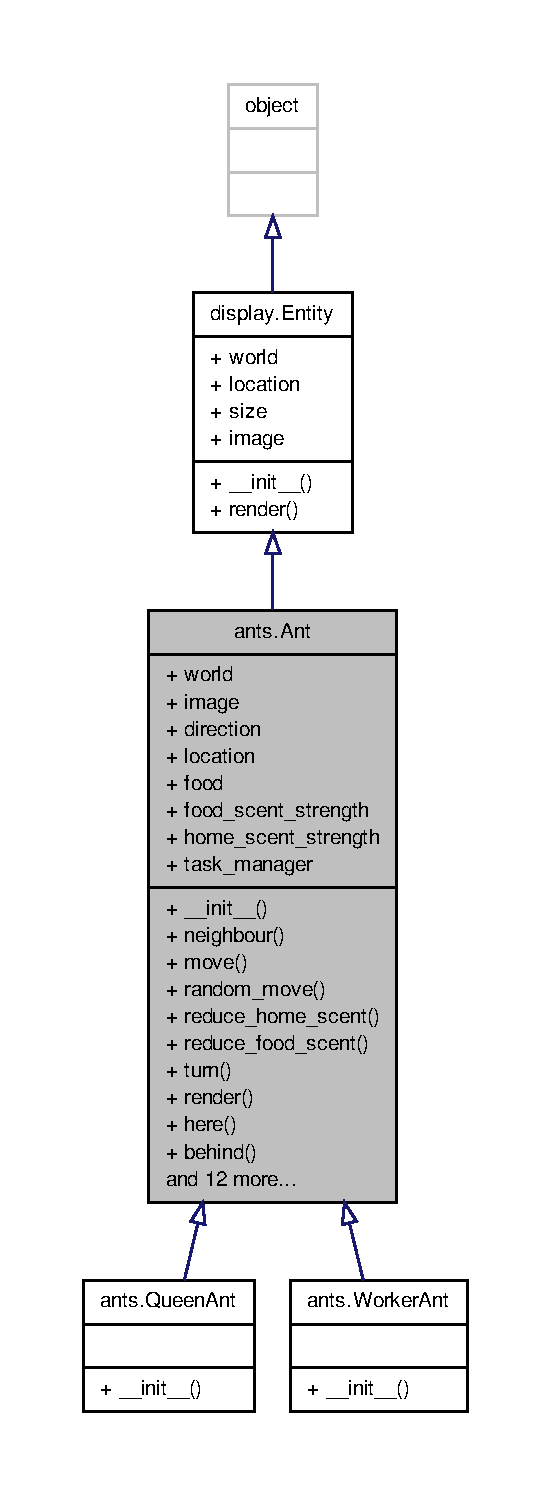
\includegraphics[height=550pt]{classants_1_1Ant__inherit__graph}
\end{center}
\end{figure}


Collaboration diagram for ants.\+Ant\+:
\nopagebreak
\begin{figure}[H]
\begin{center}
\leavevmode
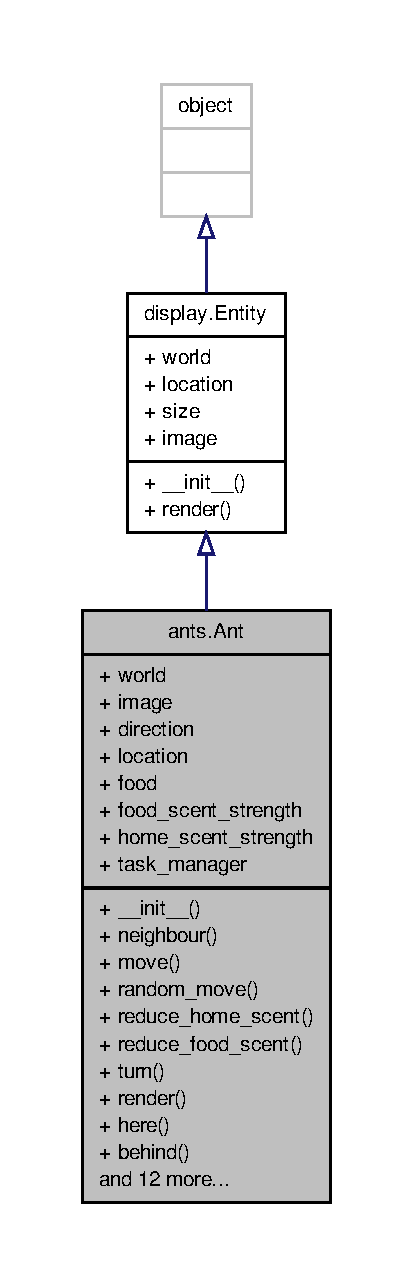
\includegraphics[height=550pt]{classants_1_1Ant__coll__graph}
\end{center}
\end{figure}
\subsection*{Public Member Functions}
\begin{DoxyCompactItemize}
\item 
def \hyperlink{classants_1_1Ant_a0fa15b6ba2860b445d390c07bc11d4e2}{\+\_\+\+\_\+init\+\_\+\+\_\+}
\item 
def \hyperlink{classants_1_1Ant_a5ee52d730c2bcbd0cfd0a8cf8d9206c6}{get\+\_\+location}
\item 
def \hyperlink{classants_1_1Ant_a2ddd97dadaa5d24c459b0117dc6e1190}{neighbour}
\item 
def \hyperlink{classants_1_1Ant_a0067159f23e5e9e4b3564d48c1564f11}{move}
\item 
def \hyperlink{classants_1_1Ant_a3a636b900b6fdbed032e3a635495a4c4}{random\+\_\+move}
\item 
def \hyperlink{classants_1_1Ant_a0f92c3c4a37d6c3998bc71fc0a6b9cee}{reduce\+\_\+home\+\_\+scent\+\_\+strength}
\item 
def \hyperlink{classants_1_1Ant_a1d51e32dc22891ded9f02ffc71e612cd}{reduce\+\_\+food\+\_\+scent\+\_\+strength}
\item 
def \hyperlink{classants_1_1Ant_a445ec1d1f8e4cb539c4f66fafa129131}{turn}
\item 
def \hyperlink{classants_1_1Ant_a95585d833c74c56155a0d79394d511cc}{render}
\item 
def \hyperlink{classants_1_1Ant_a10dc42722864d5850912dd34242d5cf8}{get\+\_\+nest\+\_\+id}
\item 
def \hyperlink{classants_1_1Ant_a2e60480b7534b107e12d7f23fd06d5f1}{here}
\item 
def \hyperlink{classants_1_1Ant_a192f8411faa05c48db8db99d033f5d15}{behind}
\item 
def \hyperlink{classants_1_1Ant_ac2c8f048d99cd48a5829ddf7ff4a708a}{ahead}
\item 
def \hyperlink{classants_1_1Ant_a2dbb07eefeecbc51d257f81fb0ba1c71}{ahead\+\_\+left}
\item 
def \hyperlink{classants_1_1Ant_ad7a5311d831e8bcc07061e6a12edad8c}{ahead\+\_\+right}
\item 
def \hyperlink{classants_1_1Ant_af9af7f8a5c766021ef0f68171d09abca}{locate\+\_\+food\+\_\+nearby}
\item 
def \hyperlink{classants_1_1Ant_aeec9c17184393435fd4d4936b6f2736a}{is\+\_\+enemy}
\begin{DoxyCompactList}\small\item\em Returns true if the ant passed is an enemy. \end{DoxyCompactList}\item 
def \hyperlink{classants_1_1Ant_a5795d0898e3d0d020a0a0a626a5ef7b0}{locate\+\_\+home\+\_\+nearby}
\item 
def \hyperlink{classants_1_1Ant_a81a141f3417ddb32b8d1abbd95bbc477}{locate\+\_\+home\+\_\+scent\+\_\+nearby}
\item 
def \hyperlink{classants_1_1Ant_a6f3e3bd98a5f382098cdc1c02e1e2fd0}{rank\+\_\+by\+\_\+home\+\_\+scent}
\item 
def \hyperlink{classants_1_1Ant_ae85884312b4aa10f965b84535bed37fc}{drop\+\_\+food}
\item 
def \hyperlink{classants_1_1Ant_accd1fa305032e848021a4d8b90f3f8ce}{take\+\_\+food}
\begin{DoxyCompactList}\small\item\em carry half the food and increase health by half the amount \end{DoxyCompactList}\item 
def \hyperlink{classants_1_1Ant_a41de1c29941a444dab25a88cbc3a881d}{has\+\_\+food}
\item 
def \hyperlink{classants_1_1Ant_ae90d1356ca3370e47c24c5fe63ebfeaf}{set\+\_\+food\+\_\+scent\+\_\+strength}
\item 
def \hyperlink{classants_1_1Ant_ae8234d6ecb9f7666e255ffa8a978355c}{set\+\_\+home\+\_\+scent\+\_\+strength}
\item 
def \hyperlink{classants_1_1Ant_a89ad26b1d79990f95979464bbd3bf9b8}{reduce\+\_\+health}
\begin{DoxyCompactList}\small\item\em Reduces the health of the ant. \end{DoxyCompactList}\item 
def \hyperlink{classants_1_1Ant_a218d9a25e9df83abf85ff596c214075c}{is\+\_\+dead}
\item 
def \hyperlink{classants_1_1Ant_a78620c709fca31c9a0b2994534082bdc}{is\+\_\+alive}
\item 
def \hyperlink{classants_1_1Ant_a16d8e187423f707e067fe2d562100437}{is\+\_\+hungry}
\item 
def \hyperlink{classants_1_1Ant_a9e4bf6309b80ab33bd628f6e7d78d013}{\+\_\+\+\_\+nonzero\+\_\+\+\_\+}
\end{DoxyCompactItemize}
\subsection*{Public Attributes}
\begin{DoxyCompactItemize}
\item 
\hyperlink{classants_1_1Ant_a55f64c7cafb3806bdcfda42586adbff5}{world}
\item 
\hyperlink{classants_1_1Ant_adf5f970b6b5e8472f42275114eeac779}{image}
\item 
\hyperlink{classants_1_1Ant_acaafd510ade5c38719b8082027162132}{nest}
\item 
\hyperlink{classants_1_1Ant_ae26b7ffd236a83d8d5c96ec6ec07b4bb}{direction}
\item 
\hyperlink{classants_1_1Ant_ae7de139b6f5bdb8d4ab42755c405ef5d}{location}
\item 
\hyperlink{classants_1_1Ant_afcfbbf8bd338401378d25c512204eb91}{food}
\item 
\hyperlink{classants_1_1Ant_aa147562276c788d4533ab63ac44d96a6}{health}
\item 
\hyperlink{classants_1_1Ant_ad7fb2ac4566880fdacfd7bf7f4ec1109}{food\+\_\+scent\+\_\+strength}
\item 
\hyperlink{classants_1_1Ant_a7885f0124adf5b10fd6fa5e8ac47edb9}{home\+\_\+scent\+\_\+strength}
\item 
\hyperlink{classants_1_1Ant_a80e2218dcfabbd9ef4d83638dd20d943}{task\+\_\+manager}
\end{DoxyCompactItemize}


\subsection{Detailed Description}
\begin{DoxyVerb}A virtual base class for Ants
\end{DoxyVerb}
 

Definition at line \hyperlink{ants_8py_source_l00008}{8} of file \hyperlink{ants_8py_source}{ants.\+py}.



\subsection{Constructor \& Destructor Documentation}
\hypertarget{classants_1_1Ant_a0fa15b6ba2860b445d390c07bc11d4e2}{\index{ants\+::\+Ant@{ants\+::\+Ant}!\+\_\+\+\_\+init\+\_\+\+\_\+@{\+\_\+\+\_\+init\+\_\+\+\_\+}}
\index{\+\_\+\+\_\+init\+\_\+\+\_\+@{\+\_\+\+\_\+init\+\_\+\+\_\+}!ants\+::\+Ant@{ants\+::\+Ant}}
\subsubsection[{\+\_\+\+\_\+init\+\_\+\+\_\+}]{\setlength{\rightskip}{0pt plus 5cm}def ants.\+Ant.\+\_\+\+\_\+init\+\_\+\+\_\+ (
\begin{DoxyParamCaption}
\item[{}]{self, }
\item[{}]{world, }
\item[{}]{image, }
\item[{}]{direction, }
\item[{}]{location, }
\item[{}]{nest}
\end{DoxyParamCaption}
)}}\label{classants_1_1Ant_a0fa15b6ba2860b445d390c07bc11d4e2}


Definition at line \hyperlink{ants_8py_source_l00012}{12} of file \hyperlink{ants_8py_source}{ants.\+py}.



\subsection{Member Function Documentation}
\hypertarget{classants_1_1Ant_a9e4bf6309b80ab33bd628f6e7d78d013}{\index{ants\+::\+Ant@{ants\+::\+Ant}!\+\_\+\+\_\+nonzero\+\_\+\+\_\+@{\+\_\+\+\_\+nonzero\+\_\+\+\_\+}}
\index{\+\_\+\+\_\+nonzero\+\_\+\+\_\+@{\+\_\+\+\_\+nonzero\+\_\+\+\_\+}!ants\+::\+Ant@{ants\+::\+Ant}}
\subsubsection[{\+\_\+\+\_\+nonzero\+\_\+\+\_\+}]{\setlength{\rightskip}{0pt plus 5cm}def ants.\+Ant.\+\_\+\+\_\+nonzero\+\_\+\+\_\+ (
\begin{DoxyParamCaption}
\item[{}]{self}
\end{DoxyParamCaption}
)}}\label{classants_1_1Ant_a9e4bf6309b80ab33bd628f6e7d78d013}


Definition at line \hyperlink{ants_8py_source_l00256}{256} of file \hyperlink{ants_8py_source}{ants.\+py}.

\hypertarget{classants_1_1Ant_ac2c8f048d99cd48a5829ddf7ff4a708a}{\index{ants\+::\+Ant@{ants\+::\+Ant}!ahead@{ahead}}
\index{ahead@{ahead}!ants\+::\+Ant@{ants\+::\+Ant}}
\subsubsection[{ahead}]{\setlength{\rightskip}{0pt plus 5cm}def ants.\+Ant.\+ahead (
\begin{DoxyParamCaption}
\item[{}]{self}
\end{DoxyParamCaption}
)}}\label{classants_1_1Ant_ac2c8f048d99cd48a5829ddf7ff4a708a}
\begin{DoxyVerb}The cell just ahead
\end{DoxyVerb}
 

Definition at line \hyperlink{ants_8py_source_l00117}{117} of file \hyperlink{ants_8py_source}{ants.\+py}.

\hypertarget{classants_1_1Ant_a2dbb07eefeecbc51d257f81fb0ba1c71}{\index{ants\+::\+Ant@{ants\+::\+Ant}!ahead\+\_\+left@{ahead\+\_\+left}}
\index{ahead\+\_\+left@{ahead\+\_\+left}!ants\+::\+Ant@{ants\+::\+Ant}}
\subsubsection[{ahead\+\_\+left}]{\setlength{\rightskip}{0pt plus 5cm}def ants.\+Ant.\+ahead\+\_\+left (
\begin{DoxyParamCaption}
\item[{}]{self}
\end{DoxyParamCaption}
)}}\label{classants_1_1Ant_a2dbb07eefeecbc51d257f81fb0ba1c71}
\begin{DoxyVerb}The cell just ahead-left
\end{DoxyVerb}
 

Definition at line \hyperlink{ants_8py_source_l00123}{123} of file \hyperlink{ants_8py_source}{ants.\+py}.

\hypertarget{classants_1_1Ant_ad7a5311d831e8bcc07061e6a12edad8c}{\index{ants\+::\+Ant@{ants\+::\+Ant}!ahead\+\_\+right@{ahead\+\_\+right}}
\index{ahead\+\_\+right@{ahead\+\_\+right}!ants\+::\+Ant@{ants\+::\+Ant}}
\subsubsection[{ahead\+\_\+right}]{\setlength{\rightskip}{0pt plus 5cm}def ants.\+Ant.\+ahead\+\_\+right (
\begin{DoxyParamCaption}
\item[{}]{self}
\end{DoxyParamCaption}
)}}\label{classants_1_1Ant_ad7a5311d831e8bcc07061e6a12edad8c}
\begin{DoxyVerb}The cell just ahead-right
\end{DoxyVerb}
 

Definition at line \hyperlink{ants_8py_source_l00129}{129} of file \hyperlink{ants_8py_source}{ants.\+py}.

\hypertarget{classants_1_1Ant_a192f8411faa05c48db8db99d033f5d15}{\index{ants\+::\+Ant@{ants\+::\+Ant}!behind@{behind}}
\index{behind@{behind}!ants\+::\+Ant@{ants\+::\+Ant}}
\subsubsection[{behind}]{\setlength{\rightskip}{0pt plus 5cm}def ants.\+Ant.\+behind (
\begin{DoxyParamCaption}
\item[{}]{self}
\end{DoxyParamCaption}
)}}\label{classants_1_1Ant_a192f8411faa05c48db8db99d033f5d15}
\begin{DoxyVerb}The cell just behind
\end{DoxyVerb}
 

Definition at line \hyperlink{ants_8py_source_l00111}{111} of file \hyperlink{ants_8py_source}{ants.\+py}.

\hypertarget{classants_1_1Ant_ae85884312b4aa10f965b84535bed37fc}{\index{ants\+::\+Ant@{ants\+::\+Ant}!drop\+\_\+food@{drop\+\_\+food}}
\index{drop\+\_\+food@{drop\+\_\+food}!ants\+::\+Ant@{ants\+::\+Ant}}
\subsubsection[{drop\+\_\+food}]{\setlength{\rightskip}{0pt plus 5cm}def ants.\+Ant.\+drop\+\_\+food (
\begin{DoxyParamCaption}
\item[{}]{self}
\end{DoxyParamCaption}
)}}\label{classants_1_1Ant_ae85884312b4aa10f965b84535bed37fc}
\begin{DoxyVerb}Set food to zero
Update the food values of the home cell it reached
\end{DoxyVerb}
 

Definition at line \hyperlink{ants_8py_source_l00214}{214} of file \hyperlink{ants_8py_source}{ants.\+py}.

\hypertarget{classants_1_1Ant_a5ee52d730c2bcbd0cfd0a8cf8d9206c6}{\index{ants\+::\+Ant@{ants\+::\+Ant}!get\+\_\+location@{get\+\_\+location}}
\index{get\+\_\+location@{get\+\_\+location}!ants\+::\+Ant@{ants\+::\+Ant}}
\subsubsection[{get\+\_\+location}]{\setlength{\rightskip}{0pt plus 5cm}def ants.\+Ant.\+get\+\_\+location (
\begin{DoxyParamCaption}
\item[{}]{self}
\end{DoxyParamCaption}
)}}\label{classants_1_1Ant_a5ee52d730c2bcbd0cfd0a8cf8d9206c6}


Definition at line \hyperlink{ants_8py_source_l00026}{26} of file \hyperlink{ants_8py_source}{ants.\+py}.

\hypertarget{classants_1_1Ant_a10dc42722864d5850912dd34242d5cf8}{\index{ants\+::\+Ant@{ants\+::\+Ant}!get\+\_\+nest\+\_\+id@{get\+\_\+nest\+\_\+id}}
\index{get\+\_\+nest\+\_\+id@{get\+\_\+nest\+\_\+id}!ants\+::\+Ant@{ants\+::\+Ant}}
\subsubsection[{get\+\_\+nest\+\_\+id}]{\setlength{\rightskip}{0pt plus 5cm}def ants.\+Ant.\+get\+\_\+nest\+\_\+id (
\begin{DoxyParamCaption}
\item[{}]{self}
\end{DoxyParamCaption}
)}}\label{classants_1_1Ant_a10dc42722864d5850912dd34242d5cf8}
\begin{DoxyVerb}Returns the id of the nest it belongs to
\end{DoxyVerb}
 

Definition at line \hyperlink{ants_8py_source_l00099}{99} of file \hyperlink{ants_8py_source}{ants.\+py}.

\hypertarget{classants_1_1Ant_a41de1c29941a444dab25a88cbc3a881d}{\index{ants\+::\+Ant@{ants\+::\+Ant}!has\+\_\+food@{has\+\_\+food}}
\index{has\+\_\+food@{has\+\_\+food}!ants\+::\+Ant@{ants\+::\+Ant}}
\subsubsection[{has\+\_\+food}]{\setlength{\rightskip}{0pt plus 5cm}def ants.\+Ant.\+has\+\_\+food (
\begin{DoxyParamCaption}
\item[{}]{self}
\end{DoxyParamCaption}
)}}\label{classants_1_1Ant_a41de1c29941a444dab25a88cbc3a881d}
\begin{DoxyVerb}Checks if the ant has food_scent
\end{DoxyVerb}
 

Definition at line \hyperlink{ants_8py_source_l00230}{230} of file \hyperlink{ants_8py_source}{ants.\+py}.

\hypertarget{classants_1_1Ant_a2e60480b7534b107e12d7f23fd06d5f1}{\index{ants\+::\+Ant@{ants\+::\+Ant}!here@{here}}
\index{here@{here}!ants\+::\+Ant@{ants\+::\+Ant}}
\subsubsection[{here}]{\setlength{\rightskip}{0pt plus 5cm}def ants.\+Ant.\+here (
\begin{DoxyParamCaption}
\item[{}]{self}
\end{DoxyParamCaption}
)}}\label{classants_1_1Ant_a2e60480b7534b107e12d7f23fd06d5f1}
\begin{DoxyVerb}The cell it is standing on
\end{DoxyVerb}
 

Definition at line \hyperlink{ants_8py_source_l00105}{105} of file \hyperlink{ants_8py_source}{ants.\+py}.

\hypertarget{classants_1_1Ant_a78620c709fca31c9a0b2994534082bdc}{\index{ants\+::\+Ant@{ants\+::\+Ant}!is\+\_\+alive@{is\+\_\+alive}}
\index{is\+\_\+alive@{is\+\_\+alive}!ants\+::\+Ant@{ants\+::\+Ant}}
\subsubsection[{is\+\_\+alive}]{\setlength{\rightskip}{0pt plus 5cm}def ants.\+Ant.\+is\+\_\+alive (
\begin{DoxyParamCaption}
\item[{}]{self}
\end{DoxyParamCaption}
)}}\label{classants_1_1Ant_a78620c709fca31c9a0b2994534082bdc}


Definition at line \hyperlink{ants_8py_source_l00250}{250} of file \hyperlink{ants_8py_source}{ants.\+py}.

\hypertarget{classants_1_1Ant_a218d9a25e9df83abf85ff596c214075c}{\index{ants\+::\+Ant@{ants\+::\+Ant}!is\+\_\+dead@{is\+\_\+dead}}
\index{is\+\_\+dead@{is\+\_\+dead}!ants\+::\+Ant@{ants\+::\+Ant}}
\subsubsection[{is\+\_\+dead}]{\setlength{\rightskip}{0pt plus 5cm}def ants.\+Ant.\+is\+\_\+dead (
\begin{DoxyParamCaption}
\item[{}]{self}
\end{DoxyParamCaption}
)}}\label{classants_1_1Ant_a218d9a25e9df83abf85ff596c214075c}


Definition at line \hyperlink{ants_8py_source_l00247}{247} of file \hyperlink{ants_8py_source}{ants.\+py}.

\hypertarget{classants_1_1Ant_aeec9c17184393435fd4d4936b6f2736a}{\index{ants\+::\+Ant@{ants\+::\+Ant}!is\+\_\+enemy@{is\+\_\+enemy}}
\index{is\+\_\+enemy@{is\+\_\+enemy}!ants\+::\+Ant@{ants\+::\+Ant}}
\subsubsection[{is\+\_\+enemy}]{\setlength{\rightskip}{0pt plus 5cm}def ants.\+Ant.\+is\+\_\+enemy (
\begin{DoxyParamCaption}
\item[{}]{self, }
\item[{}]{ant}
\end{DoxyParamCaption}
)}}\label{classants_1_1Ant_aeec9c17184393435fd4d4936b6f2736a}


Returns true if the ant passed is an enemy. 


\begin{DoxyParams}{Parameters}
{\em ant} & The other ant \\
\hline
\end{DoxyParams}


Definition at line \hyperlink{ants_8py_source_l00155}{155} of file \hyperlink{ants_8py_source}{ants.\+py}.

\hypertarget{classants_1_1Ant_a16d8e187423f707e067fe2d562100437}{\index{ants\+::\+Ant@{ants\+::\+Ant}!is\+\_\+hungry@{is\+\_\+hungry}}
\index{is\+\_\+hungry@{is\+\_\+hungry}!ants\+::\+Ant@{ants\+::\+Ant}}
\subsubsection[{is\+\_\+hungry}]{\setlength{\rightskip}{0pt plus 5cm}def ants.\+Ant.\+is\+\_\+hungry (
\begin{DoxyParamCaption}
\item[{}]{self}
\end{DoxyParamCaption}
)}}\label{classants_1_1Ant_a16d8e187423f707e067fe2d562100437}


Definition at line \hyperlink{ants_8py_source_l00253}{253} of file \hyperlink{ants_8py_source}{ants.\+py}.

\hypertarget{classants_1_1Ant_af9af7f8a5c766021ef0f68171d09abca}{\index{ants\+::\+Ant@{ants\+::\+Ant}!locate\+\_\+food\+\_\+nearby@{locate\+\_\+food\+\_\+nearby}}
\index{locate\+\_\+food\+\_\+nearby@{locate\+\_\+food\+\_\+nearby}!ants\+::\+Ant@{ants\+::\+Ant}}
\subsubsection[{locate\+\_\+food\+\_\+nearby}]{\setlength{\rightskip}{0pt plus 5cm}def ants.\+Ant.\+locate\+\_\+food\+\_\+nearby (
\begin{DoxyParamCaption}
\item[{}]{self}
\end{DoxyParamCaption}
)}}\label{classants_1_1Ant_af9af7f8a5c766021ef0f68171d09abca}
\begin{DoxyVerb}Locate all sources nearby and return any one randomly
return None if no food source is found
\end{DoxyVerb}
 

Definition at line \hyperlink{ants_8py_source_l00135}{135} of file \hyperlink{ants_8py_source}{ants.\+py}.

\hypertarget{classants_1_1Ant_a5795d0898e3d0d020a0a0a626a5ef7b0}{\index{ants\+::\+Ant@{ants\+::\+Ant}!locate\+\_\+home\+\_\+nearby@{locate\+\_\+home\+\_\+nearby}}
\index{locate\+\_\+home\+\_\+nearby@{locate\+\_\+home\+\_\+nearby}!ants\+::\+Ant@{ants\+::\+Ant}}
\subsubsection[{locate\+\_\+home\+\_\+nearby}]{\setlength{\rightskip}{0pt plus 5cm}def ants.\+Ant.\+locate\+\_\+home\+\_\+nearby (
\begin{DoxyParamCaption}
\item[{}]{self}
\end{DoxyParamCaption}
)}}\label{classants_1_1Ant_a5795d0898e3d0d020a0a0a626a5ef7b0}
\begin{DoxyVerb}Locate home cell nearby and return any one randomly
return None if not found
\end{DoxyVerb}
 

Definition at line \hyperlink{ants_8py_source_l00158}{158} of file \hyperlink{ants_8py_source}{ants.\+py}.

\hypertarget{classants_1_1Ant_a81a141f3417ddb32b8d1abbd95bbc477}{\index{ants\+::\+Ant@{ants\+::\+Ant}!locate\+\_\+home\+\_\+scent\+\_\+nearby@{locate\+\_\+home\+\_\+scent\+\_\+nearby}}
\index{locate\+\_\+home\+\_\+scent\+\_\+nearby@{locate\+\_\+home\+\_\+scent\+\_\+nearby}!ants\+::\+Ant@{ants\+::\+Ant}}
\subsubsection[{locate\+\_\+home\+\_\+scent\+\_\+nearby}]{\setlength{\rightskip}{0pt plus 5cm}def ants.\+Ant.\+locate\+\_\+home\+\_\+scent\+\_\+nearby (
\begin{DoxyParamCaption}
\item[{}]{self}
\end{DoxyParamCaption}
)}}\label{classants_1_1Ant_a81a141f3417ddb32b8d1abbd95bbc477}
\begin{DoxyVerb}Scan the 5 directions near the direction of the ant for home scent and
return one random direction
return None if not found
\end{DoxyVerb}
 

Definition at line \hyperlink{ants_8py_source_l00176}{176} of file \hyperlink{ants_8py_source}{ants.\+py}.

\hypertarget{classants_1_1Ant_a0067159f23e5e9e4b3564d48c1564f11}{\index{ants\+::\+Ant@{ants\+::\+Ant}!move@{move}}
\index{move@{move}!ants\+::\+Ant@{ants\+::\+Ant}}
\subsubsection[{move}]{\setlength{\rightskip}{0pt plus 5cm}def ants.\+Ant.\+move (
\begin{DoxyParamCaption}
\item[{}]{self}
\end{DoxyParamCaption}
)}}\label{classants_1_1Ant_a0067159f23e5e9e4b3564d48c1564f11}
\begin{DoxyVerb}Moves the ant by a unit if the next cell is empty,
otherwise turn by an unit
It also leaves a scent trail,
remove the ant from its old cell, and
update the current cell ant with itself
\end{DoxyVerb}
 

Definition at line \hyperlink{ants_8py_source_l00038}{38} of file \hyperlink{ants_8py_source}{ants.\+py}.

\hypertarget{classants_1_1Ant_a2ddd97dadaa5d24c459b0117dc6e1190}{\index{ants\+::\+Ant@{ants\+::\+Ant}!neighbour@{neighbour}}
\index{neighbour@{neighbour}!ants\+::\+Ant@{ants\+::\+Ant}}
\subsubsection[{neighbour}]{\setlength{\rightskip}{0pt plus 5cm}def ants.\+Ant.\+neighbour (
\begin{DoxyParamCaption}
\item[{}]{self, }
\item[{}]{direction}
\end{DoxyParamCaption}
)}}\label{classants_1_1Ant_a2ddd97dadaa5d24c459b0117dc6e1190}
\begin{DoxyVerb}Returns location of neighbouring cell in a direction 
relative to the ant direction
\end{DoxyVerb}
 

Definition at line \hyperlink{ants_8py_source_l00029}{29} of file \hyperlink{ants_8py_source}{ants.\+py}.

\hypertarget{classants_1_1Ant_a3a636b900b6fdbed032e3a635495a4c4}{\index{ants\+::\+Ant@{ants\+::\+Ant}!random\+\_\+move@{random\+\_\+move}}
\index{random\+\_\+move@{random\+\_\+move}!ants\+::\+Ant@{ants\+::\+Ant}}
\subsubsection[{random\+\_\+move}]{\setlength{\rightskip}{0pt plus 5cm}def ants.\+Ant.\+random\+\_\+move (
\begin{DoxyParamCaption}
\item[{}]{self}
\end{DoxyParamCaption}
)}}\label{classants_1_1Ant_a3a636b900b6fdbed032e3a635495a4c4}
\begin{DoxyVerb}Ant makes a move forward or turns randomly
\end{DoxyVerb}
 

Definition at line \hyperlink{ants_8py_source_l00060}{60} of file \hyperlink{ants_8py_source}{ants.\+py}.

\hypertarget{classants_1_1Ant_a6f3e3bd98a5f382098cdc1c02e1e2fd0}{\index{ants\+::\+Ant@{ants\+::\+Ant}!rank\+\_\+by\+\_\+home\+\_\+scent@{rank\+\_\+by\+\_\+home\+\_\+scent}}
\index{rank\+\_\+by\+\_\+home\+\_\+scent@{rank\+\_\+by\+\_\+home\+\_\+scent}!ants\+::\+Ant@{ants\+::\+Ant}}
\subsubsection[{rank\+\_\+by\+\_\+home\+\_\+scent}]{\setlength{\rightskip}{0pt plus 5cm}def ants.\+Ant.\+rank\+\_\+by\+\_\+home\+\_\+scent (
\begin{DoxyParamCaption}
\item[{}]{self}
\end{DoxyParamCaption}
)}}\label{classants_1_1Ant_a6f3e3bd98a5f382098cdc1c02e1e2fd0}
\begin{DoxyVerb}Scan the 5 directions near the direction of the ant for home scent and
return the direction with the strongest scent
return None if not found
\end{DoxyVerb}
 

Definition at line \hyperlink{ants_8py_source_l00196}{196} of file \hyperlink{ants_8py_source}{ants.\+py}.

\hypertarget{classants_1_1Ant_a1d51e32dc22891ded9f02ffc71e612cd}{\index{ants\+::\+Ant@{ants\+::\+Ant}!reduce\+\_\+food\+\_\+scent\+\_\+strength@{reduce\+\_\+food\+\_\+scent\+\_\+strength}}
\index{reduce\+\_\+food\+\_\+scent\+\_\+strength@{reduce\+\_\+food\+\_\+scent\+\_\+strength}!ants\+::\+Ant@{ants\+::\+Ant}}
\subsubsection[{reduce\+\_\+food\+\_\+scent\+\_\+strength}]{\setlength{\rightskip}{0pt plus 5cm}def ants.\+Ant.\+reduce\+\_\+food\+\_\+scent\+\_\+strength (
\begin{DoxyParamCaption}
\item[{}]{self, }
\item[{}]{amt = {\ttfamily 1}}
\end{DoxyParamCaption}
)}}\label{classants_1_1Ant_a1d51e32dc22891ded9f02ffc71e612cd}
\begin{DoxyVerb}Reduce food scent by 'amt'
\end{DoxyVerb}
 

Definition at line \hyperlink{ants_8py_source_l00076}{76} of file \hyperlink{ants_8py_source}{ants.\+py}.

\hypertarget{classants_1_1Ant_a89ad26b1d79990f95979464bbd3bf9b8}{\index{ants\+::\+Ant@{ants\+::\+Ant}!reduce\+\_\+health@{reduce\+\_\+health}}
\index{reduce\+\_\+health@{reduce\+\_\+health}!ants\+::\+Ant@{ants\+::\+Ant}}
\subsubsection[{reduce\+\_\+health}]{\setlength{\rightskip}{0pt plus 5cm}def ants.\+Ant.\+reduce\+\_\+health (
\begin{DoxyParamCaption}
\item[{}]{self, }
\item[{}]{amt}
\end{DoxyParamCaption}
)}}\label{classants_1_1Ant_a89ad26b1d79990f95979464bbd3bf9b8}


Reduces the health of the ant. 


\begin{DoxyParams}{Parameters}
{\em amt} & The amount of health to reduce \\
\hline
\end{DoxyParams}


Definition at line \hyperlink{ants_8py_source_l00244}{244} of file \hyperlink{ants_8py_source}{ants.\+py}.

\hypertarget{classants_1_1Ant_a0f92c3c4a37d6c3998bc71fc0a6b9cee}{\index{ants\+::\+Ant@{ants\+::\+Ant}!reduce\+\_\+home\+\_\+scent\+\_\+strength@{reduce\+\_\+home\+\_\+scent\+\_\+strength}}
\index{reduce\+\_\+home\+\_\+scent\+\_\+strength@{reduce\+\_\+home\+\_\+scent\+\_\+strength}!ants\+::\+Ant@{ants\+::\+Ant}}
\subsubsection[{reduce\+\_\+home\+\_\+scent\+\_\+strength}]{\setlength{\rightskip}{0pt plus 5cm}def ants.\+Ant.\+reduce\+\_\+home\+\_\+scent\+\_\+strength (
\begin{DoxyParamCaption}
\item[{}]{self, }
\item[{}]{amt = {\ttfamily 1}}
\end{DoxyParamCaption}
)}}\label{classants_1_1Ant_a0f92c3c4a37d6c3998bc71fc0a6b9cee}
\begin{DoxyVerb}Reduce home scent by 'amt'
\end{DoxyVerb}
 

Definition at line \hyperlink{ants_8py_source_l00069}{69} of file \hyperlink{ants_8py_source}{ants.\+py}.

\hypertarget{classants_1_1Ant_a95585d833c74c56155a0d79394d511cc}{\index{ants\+::\+Ant@{ants\+::\+Ant}!render@{render}}
\index{render@{render}!ants\+::\+Ant@{ants\+::\+Ant}}
\subsubsection[{render}]{\setlength{\rightskip}{0pt plus 5cm}def ants.\+Ant.\+render (
\begin{DoxyParamCaption}
\item[{}]{self}
\end{DoxyParamCaption}
)}}\label{classants_1_1Ant_a95585d833c74c56155a0d79394d511cc}
\begin{DoxyVerb}Render itself
\end{DoxyVerb}
 

Definition at line \hyperlink{ants_8py_source_l00089}{89} of file \hyperlink{ants_8py_source}{ants.\+py}.

\hypertarget{classants_1_1Ant_ae90d1356ca3370e47c24c5fe63ebfeaf}{\index{ants\+::\+Ant@{ants\+::\+Ant}!set\+\_\+food\+\_\+scent\+\_\+strength@{set\+\_\+food\+\_\+scent\+\_\+strength}}
\index{set\+\_\+food\+\_\+scent\+\_\+strength@{set\+\_\+food\+\_\+scent\+\_\+strength}!ants\+::\+Ant@{ants\+::\+Ant}}
\subsubsection[{set\+\_\+food\+\_\+scent\+\_\+strength}]{\setlength{\rightskip}{0pt plus 5cm}def ants.\+Ant.\+set\+\_\+food\+\_\+scent\+\_\+strength (
\begin{DoxyParamCaption}
\item[{}]{self, }
\item[{}]{strength}
\end{DoxyParamCaption}
)}}\label{classants_1_1Ant_ae90d1356ca3370e47c24c5fe63ebfeaf}


Definition at line \hyperlink{ants_8py_source_l00236}{236} of file \hyperlink{ants_8py_source}{ants.\+py}.

\hypertarget{classants_1_1Ant_ae8234d6ecb9f7666e255ffa8a978355c}{\index{ants\+::\+Ant@{ants\+::\+Ant}!set\+\_\+home\+\_\+scent\+\_\+strength@{set\+\_\+home\+\_\+scent\+\_\+strength}}
\index{set\+\_\+home\+\_\+scent\+\_\+strength@{set\+\_\+home\+\_\+scent\+\_\+strength}!ants\+::\+Ant@{ants\+::\+Ant}}
\subsubsection[{set\+\_\+home\+\_\+scent\+\_\+strength}]{\setlength{\rightskip}{0pt plus 5cm}def ants.\+Ant.\+set\+\_\+home\+\_\+scent\+\_\+strength (
\begin{DoxyParamCaption}
\item[{}]{self, }
\item[{}]{strength}
\end{DoxyParamCaption}
)}}\label{classants_1_1Ant_ae8234d6ecb9f7666e255ffa8a978355c}


Definition at line \hyperlink{ants_8py_source_l00239}{239} of file \hyperlink{ants_8py_source}{ants.\+py}.

\hypertarget{classants_1_1Ant_accd1fa305032e848021a4d8b90f3f8ce}{\index{ants\+::\+Ant@{ants\+::\+Ant}!take\+\_\+food@{take\+\_\+food}}
\index{take\+\_\+food@{take\+\_\+food}!ants\+::\+Ant@{ants\+::\+Ant}}
\subsubsection[{take\+\_\+food}]{\setlength{\rightskip}{0pt plus 5cm}def ants.\+Ant.\+take\+\_\+food (
\begin{DoxyParamCaption}
\item[{}]{self, }
\item[{}]{amt}
\end{DoxyParamCaption}
)}}\label{classants_1_1Ant_accd1fa305032e848021a4d8b90f3f8ce}


carry half the food and increase health by half the amount 


\begin{DoxyParams}{Parameters}
{\em amt} & The amount of food \\
\hline
\end{DoxyParams}


Definition at line \hyperlink{ants_8py_source_l00226}{226} of file \hyperlink{ants_8py_source}{ants.\+py}.

\hypertarget{classants_1_1Ant_a445ec1d1f8e4cb539c4f66fafa129131}{\index{ants\+::\+Ant@{ants\+::\+Ant}!turn@{turn}}
\index{turn@{turn}!ants\+::\+Ant@{ants\+::\+Ant}}
\subsubsection[{turn}]{\setlength{\rightskip}{0pt plus 5cm}def ants.\+Ant.\+turn (
\begin{DoxyParamCaption}
\item[{}]{self, }
\item[{}]{n}
\end{DoxyParamCaption}
)}}\label{classants_1_1Ant_a445ec1d1f8e4cb539c4f66fafa129131}
\begin{DoxyVerb}Changes direction n times
\end{DoxyVerb}
 

Definition at line \hyperlink{ants_8py_source_l00083}{83} of file \hyperlink{ants_8py_source}{ants.\+py}.



\subsection{Member Data Documentation}
\hypertarget{classants_1_1Ant_ae26b7ffd236a83d8d5c96ec6ec07b4bb}{\index{ants\+::\+Ant@{ants\+::\+Ant}!direction@{direction}}
\index{direction@{direction}!ants\+::\+Ant@{ants\+::\+Ant}}
\subsubsection[{direction}]{\setlength{\rightskip}{0pt plus 5cm}ants.\+Ant.\+direction}}\label{classants_1_1Ant_ae26b7ffd236a83d8d5c96ec6ec07b4bb}


Definition at line \hyperlink{ants_8py_source_l00017}{17} of file \hyperlink{ants_8py_source}{ants.\+py}.

\hypertarget{classants_1_1Ant_afcfbbf8bd338401378d25c512204eb91}{\index{ants\+::\+Ant@{ants\+::\+Ant}!food@{food}}
\index{food@{food}!ants\+::\+Ant@{ants\+::\+Ant}}
\subsubsection[{food}]{\setlength{\rightskip}{0pt plus 5cm}ants.\+Ant.\+food}}\label{classants_1_1Ant_afcfbbf8bd338401378d25c512204eb91}


Definition at line \hyperlink{ants_8py_source_l00019}{19} of file \hyperlink{ants_8py_source}{ants.\+py}.

\hypertarget{classants_1_1Ant_ad7fb2ac4566880fdacfd7bf7f4ec1109}{\index{ants\+::\+Ant@{ants\+::\+Ant}!food\+\_\+scent\+\_\+strength@{food\+\_\+scent\+\_\+strength}}
\index{food\+\_\+scent\+\_\+strength@{food\+\_\+scent\+\_\+strength}!ants\+::\+Ant@{ants\+::\+Ant}}
\subsubsection[{food\+\_\+scent\+\_\+strength}]{\setlength{\rightskip}{0pt plus 5cm}ants.\+Ant.\+food\+\_\+scent\+\_\+strength}}\label{classants_1_1Ant_ad7fb2ac4566880fdacfd7bf7f4ec1109}


Definition at line \hyperlink{ants_8py_source_l00021}{21} of file \hyperlink{ants_8py_source}{ants.\+py}.

\hypertarget{classants_1_1Ant_aa147562276c788d4533ab63ac44d96a6}{\index{ants\+::\+Ant@{ants\+::\+Ant}!health@{health}}
\index{health@{health}!ants\+::\+Ant@{ants\+::\+Ant}}
\subsubsection[{health}]{\setlength{\rightskip}{0pt plus 5cm}ants.\+Ant.\+health}}\label{classants_1_1Ant_aa147562276c788d4533ab63ac44d96a6}


Definition at line \hyperlink{ants_8py_source_l00020}{20} of file \hyperlink{ants_8py_source}{ants.\+py}.

\hypertarget{classants_1_1Ant_a7885f0124adf5b10fd6fa5e8ac47edb9}{\index{ants\+::\+Ant@{ants\+::\+Ant}!home\+\_\+scent\+\_\+strength@{home\+\_\+scent\+\_\+strength}}
\index{home\+\_\+scent\+\_\+strength@{home\+\_\+scent\+\_\+strength}!ants\+::\+Ant@{ants\+::\+Ant}}
\subsubsection[{home\+\_\+scent\+\_\+strength}]{\setlength{\rightskip}{0pt plus 5cm}ants.\+Ant.\+home\+\_\+scent\+\_\+strength}}\label{classants_1_1Ant_a7885f0124adf5b10fd6fa5e8ac47edb9}


Definition at line \hyperlink{ants_8py_source_l00022}{22} of file \hyperlink{ants_8py_source}{ants.\+py}.

\hypertarget{classants_1_1Ant_adf5f970b6b5e8472f42275114eeac779}{\index{ants\+::\+Ant@{ants\+::\+Ant}!image@{image}}
\index{image@{image}!ants\+::\+Ant@{ants\+::\+Ant}}
\subsubsection[{image}]{\setlength{\rightskip}{0pt plus 5cm}ants.\+Ant.\+image}}\label{classants_1_1Ant_adf5f970b6b5e8472f42275114eeac779}


Definition at line \hyperlink{ants_8py_source_l00015}{15} of file \hyperlink{ants_8py_source}{ants.\+py}.

\hypertarget{classants_1_1Ant_ae7de139b6f5bdb8d4ab42755c405ef5d}{\index{ants\+::\+Ant@{ants\+::\+Ant}!location@{location}}
\index{location@{location}!ants\+::\+Ant@{ants\+::\+Ant}}
\subsubsection[{location}]{\setlength{\rightskip}{0pt plus 5cm}ants.\+Ant.\+location}}\label{classants_1_1Ant_ae7de139b6f5bdb8d4ab42755c405ef5d}


Definition at line \hyperlink{ants_8py_source_l00018}{18} of file \hyperlink{ants_8py_source}{ants.\+py}.

\hypertarget{classants_1_1Ant_acaafd510ade5c38719b8082027162132}{\index{ants\+::\+Ant@{ants\+::\+Ant}!nest@{nest}}
\index{nest@{nest}!ants\+::\+Ant@{ants\+::\+Ant}}
\subsubsection[{nest}]{\setlength{\rightskip}{0pt plus 5cm}ants.\+Ant.\+nest}}\label{classants_1_1Ant_acaafd510ade5c38719b8082027162132}


Definition at line \hyperlink{ants_8py_source_l00016}{16} of file \hyperlink{ants_8py_source}{ants.\+py}.

\hypertarget{classants_1_1Ant_a80e2218dcfabbd9ef4d83638dd20d943}{\index{ants\+::\+Ant@{ants\+::\+Ant}!task\+\_\+manager@{task\+\_\+manager}}
\index{task\+\_\+manager@{task\+\_\+manager}!ants\+::\+Ant@{ants\+::\+Ant}}
\subsubsection[{task\+\_\+manager}]{\setlength{\rightskip}{0pt plus 5cm}ants.\+Ant.\+task\+\_\+manager}}\label{classants_1_1Ant_a80e2218dcfabbd9ef4d83638dd20d943}


Definition at line \hyperlink{ants_8py_source_l00024}{24} of file \hyperlink{ants_8py_source}{ants.\+py}.

\hypertarget{classants_1_1Ant_a55f64c7cafb3806bdcfda42586adbff5}{\index{ants\+::\+Ant@{ants\+::\+Ant}!world@{world}}
\index{world@{world}!ants\+::\+Ant@{ants\+::\+Ant}}
\subsubsection[{world}]{\setlength{\rightskip}{0pt plus 5cm}ants.\+Ant.\+world}}\label{classants_1_1Ant_a55f64c7cafb3806bdcfda42586adbff5}


Definition at line \hyperlink{ants_8py_source_l00014}{14} of file \hyperlink{ants_8py_source}{ants.\+py}.



The documentation for this class was generated from the following file\+:\begin{DoxyCompactItemize}
\item 
\hyperlink{ants_8py}{ants.\+py}\end{DoxyCompactItemize}

\hypertarget{classworld_1_1Cell}{\section{world.\+Cell Class Reference}
\label{classworld_1_1Cell}\index{world.\+Cell@{world.\+Cell}}
}


Inheritance diagram for world.\+Cell\+:\nopagebreak
\begin{figure}[H]
\begin{center}
\leavevmode
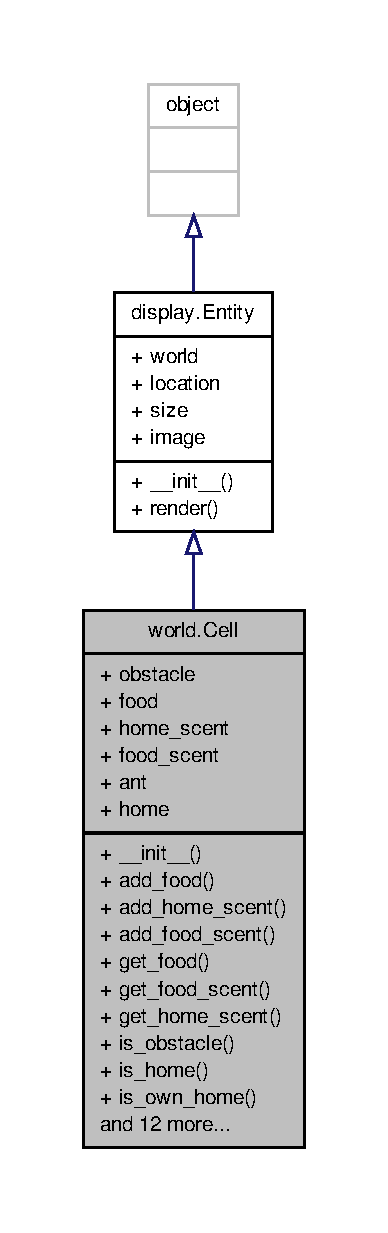
\includegraphics[height=550pt]{classworld_1_1Cell__inherit__graph}
\end{center}
\end{figure}


Collaboration diagram for world.\+Cell\+:\nopagebreak
\begin{figure}[H]
\begin{center}
\leavevmode
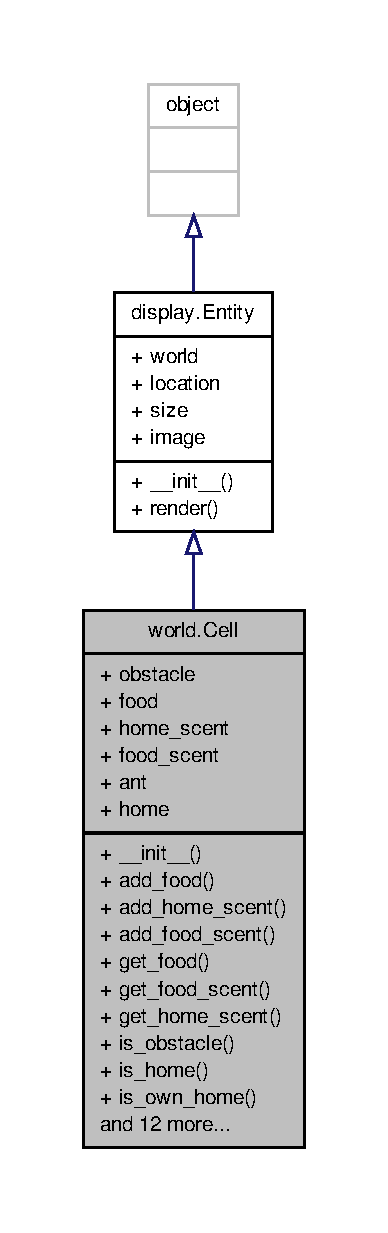
\includegraphics[height=550pt]{classworld_1_1Cell__coll__graph}
\end{center}
\end{figure}
\subsection*{Public Member Functions}
\begin{DoxyCompactItemize}
\item 
def \hyperlink{classworld_1_1Cell_a3dd387b6af13f7450acb97fb40c13a0e}{\+\_\+\+\_\+init\+\_\+\+\_\+}
\item 
def \hyperlink{classworld_1_1Cell_a3d9725f56b584acd9f75728f364975b0}{add\+\_\+food}
\item 
def \hyperlink{classworld_1_1Cell_a52af74786918c6c3f4d1d0b0f44aecb8}{add\+\_\+home\+\_\+scent}
\item 
def \hyperlink{classworld_1_1Cell_a773c26b2353ffaede745ee726d2e256d}{add\+\_\+food\+\_\+scent}
\item 
def \hyperlink{classworld_1_1Cell_ace4b7ca65667e6dcecb3c43e850c3568}{get\+\_\+food}
\item 
def \hyperlink{classworld_1_1Cell_a890e2dc899a32ef86c131a98879e9023}{is\+\_\+obstacle}
\item 
def \hyperlink{classworld_1_1Cell_a441597e0ea2cff7fce907a12fd8216fa}{is\+\_\+home}
\item 
def \hyperlink{classworld_1_1Cell_a90eabca5d79eef89b2ae4f677a88a93b}{is\+\_\+food}
\item 
def \hyperlink{classworld_1_1Cell_a98e3cac3c42374693afe0aded7a1e06c}{has\+\_\+ant}
\item 
def \hyperlink{classworld_1_1Cell_a1097df1a6fe0131898377358017fe7bc}{has\+\_\+food}
\item 
def \hyperlink{classworld_1_1Cell_adb830df07e437189375efa6c9ad4981e}{make\+\_\+home}
\item 
def \hyperlink{classworld_1_1Cell_a63164a3e74888a97b07ee8e06c633c2a}{make\+\_\+obstacle}
\item 
def \hyperlink{classworld_1_1Cell_add0fb2c9e6c963d012cf7e65008b8947}{evaporate\+\_\+scent}
\item 
def \hyperlink{classworld_1_1Cell_a11f263897c7a04ae900af84d30a30c56}{render}
\end{DoxyCompactItemize}
\subsection*{Public Attributes}
\begin{DoxyCompactItemize}
\item 
\hyperlink{classworld_1_1Cell_aeaf17388b8c9000fe612ab043418825c}{obstacle}
\item 
\hyperlink{classworld_1_1Cell_a401fde7236825c1843dad8764c2fb4a8}{food}
\item 
\hyperlink{classworld_1_1Cell_a0ef4adaadea1ccdcd1b61c70e242aa4a}{home\+\_\+scent}
\item 
\hyperlink{classworld_1_1Cell_acec0cb9d8a7eb92bedf71dc57641efbe}{food\+\_\+scent}
\item 
\hyperlink{classworld_1_1Cell_abfd9b278ac86f77970b7766a7c2e3231}{ant}
\item 
\hyperlink{classworld_1_1Cell_a9baf3378be8090bf1faf1b19b9aa5fd3}{home}
\end{DoxyCompactItemize}


\subsection{Detailed Description}
\begin{DoxyVerb}Data containers for each location in World\end{DoxyVerb}
 

Definition at line \hyperlink{world_8py_source_l00008}{8} of file \hyperlink{world_8py_source}{world.\+py}.



\subsection{Constructor \& Destructor Documentation}
\hypertarget{classworld_1_1Cell_a3dd387b6af13f7450acb97fb40c13a0e}{\index{world\+::\+Cell@{world\+::\+Cell}!\+\_\+\+\_\+init\+\_\+\+\_\+@{\+\_\+\+\_\+init\+\_\+\+\_\+}}
\index{\+\_\+\+\_\+init\+\_\+\+\_\+@{\+\_\+\+\_\+init\+\_\+\+\_\+}!world\+::\+Cell@{world\+::\+Cell}}
\subsubsection[{\+\_\+\+\_\+init\+\_\+\+\_\+}]{\setlength{\rightskip}{0pt plus 5cm}def world.\+Cell.\+\_\+\+\_\+init\+\_\+\+\_\+ (
\begin{DoxyParamCaption}
\item[{}]{self, }
\item[{}]{world, }
\item[{}]{i, }
\item[{}]{j, }
\item[{}]{cell\+\_\+size}
\end{DoxyParamCaption}
)}}\label{classworld_1_1Cell_a3dd387b6af13f7450acb97fb40c13a0e}


Definition at line \hyperlink{world_8py_source_l00010}{10} of file \hyperlink{world_8py_source}{world.\+py}.



\subsection{Member Function Documentation}
\hypertarget{classworld_1_1Cell_a3d9725f56b584acd9f75728f364975b0}{\index{world\+::\+Cell@{world\+::\+Cell}!add\+\_\+food@{add\+\_\+food}}
\index{add\+\_\+food@{add\+\_\+food}!world\+::\+Cell@{world\+::\+Cell}}
\subsubsection[{add\+\_\+food}]{\setlength{\rightskip}{0pt plus 5cm}def world.\+Cell.\+add\+\_\+food (
\begin{DoxyParamCaption}
\item[{}]{self, }
\item[{}]{amt}
\end{DoxyParamCaption}
)}}\label{classworld_1_1Cell_a3d9725f56b584acd9f75728f364975b0}


Definition at line \hyperlink{world_8py_source_l00019}{19} of file \hyperlink{world_8py_source}{world.\+py}.

\hypertarget{classworld_1_1Cell_a773c26b2353ffaede745ee726d2e256d}{\index{world\+::\+Cell@{world\+::\+Cell}!add\+\_\+food\+\_\+scent@{add\+\_\+food\+\_\+scent}}
\index{add\+\_\+food\+\_\+scent@{add\+\_\+food\+\_\+scent}!world\+::\+Cell@{world\+::\+Cell}}
\subsubsection[{add\+\_\+food\+\_\+scent}]{\setlength{\rightskip}{0pt plus 5cm}def world.\+Cell.\+add\+\_\+food\+\_\+scent (
\begin{DoxyParamCaption}
\item[{}]{self, }
\item[{}]{amt}
\end{DoxyParamCaption}
)}}\label{classworld_1_1Cell_a773c26b2353ffaede745ee726d2e256d}


Definition at line \hyperlink{world_8py_source_l00025}{25} of file \hyperlink{world_8py_source}{world.\+py}.

\hypertarget{classworld_1_1Cell_a52af74786918c6c3f4d1d0b0f44aecb8}{\index{world\+::\+Cell@{world\+::\+Cell}!add\+\_\+home\+\_\+scent@{add\+\_\+home\+\_\+scent}}
\index{add\+\_\+home\+\_\+scent@{add\+\_\+home\+\_\+scent}!world\+::\+Cell@{world\+::\+Cell}}
\subsubsection[{add\+\_\+home\+\_\+scent}]{\setlength{\rightskip}{0pt plus 5cm}def world.\+Cell.\+add\+\_\+home\+\_\+scent (
\begin{DoxyParamCaption}
\item[{}]{self, }
\item[{}]{amt}
\end{DoxyParamCaption}
)}}\label{classworld_1_1Cell_a52af74786918c6c3f4d1d0b0f44aecb8}


Definition at line \hyperlink{world_8py_source_l00022}{22} of file \hyperlink{world_8py_source}{world.\+py}.

\hypertarget{classworld_1_1Cell_add0fb2c9e6c963d012cf7e65008b8947}{\index{world\+::\+Cell@{world\+::\+Cell}!evaporate\+\_\+scent@{evaporate\+\_\+scent}}
\index{evaporate\+\_\+scent@{evaporate\+\_\+scent}!world\+::\+Cell@{world\+::\+Cell}}
\subsubsection[{evaporate\+\_\+scent}]{\setlength{\rightskip}{0pt plus 5cm}def world.\+Cell.\+evaporate\+\_\+scent (
\begin{DoxyParamCaption}
\item[{}]{self, }
\item[{}]{rate}
\end{DoxyParamCaption}
)}}\label{classworld_1_1Cell_add0fb2c9e6c963d012cf7e65008b8947}
\begin{DoxyVerb}Evaporates scent ( decay law )\end{DoxyVerb}
 

Definition at line \hyperlink{world_8py_source_l00059}{59} of file \hyperlink{world_8py_source}{world.\+py}.

\hypertarget{classworld_1_1Cell_ace4b7ca65667e6dcecb3c43e850c3568}{\index{world\+::\+Cell@{world\+::\+Cell}!get\+\_\+food@{get\+\_\+food}}
\index{get\+\_\+food@{get\+\_\+food}!world\+::\+Cell@{world\+::\+Cell}}
\subsubsection[{get\+\_\+food}]{\setlength{\rightskip}{0pt plus 5cm}def world.\+Cell.\+get\+\_\+food (
\begin{DoxyParamCaption}
\item[{}]{self, }
\item[{}]{amt}
\end{DoxyParamCaption}
)}}\label{classworld_1_1Cell_ace4b7ca65667e6dcecb3c43e850c3568}
\begin{DoxyVerb}Get "amt" amount of food if available else returns whatever food is available\end{DoxyVerb}
 

Definition at line \hyperlink{world_8py_source_l00028}{28} of file \hyperlink{world_8py_source}{world.\+py}.

\hypertarget{classworld_1_1Cell_a98e3cac3c42374693afe0aded7a1e06c}{\index{world\+::\+Cell@{world\+::\+Cell}!has\+\_\+ant@{has\+\_\+ant}}
\index{has\+\_\+ant@{has\+\_\+ant}!world\+::\+Cell@{world\+::\+Cell}}
\subsubsection[{has\+\_\+ant}]{\setlength{\rightskip}{0pt plus 5cm}def world.\+Cell.\+has\+\_\+ant (
\begin{DoxyParamCaption}
\item[{}]{self}
\end{DoxyParamCaption}
)}}\label{classworld_1_1Cell_a98e3cac3c42374693afe0aded7a1e06c}


Definition at line \hyperlink{world_8py_source_l00047}{47} of file \hyperlink{world_8py_source}{world.\+py}.

\hypertarget{classworld_1_1Cell_a1097df1a6fe0131898377358017fe7bc}{\index{world\+::\+Cell@{world\+::\+Cell}!has\+\_\+food@{has\+\_\+food}}
\index{has\+\_\+food@{has\+\_\+food}!world\+::\+Cell@{world\+::\+Cell}}
\subsubsection[{has\+\_\+food}]{\setlength{\rightskip}{0pt plus 5cm}def world.\+Cell.\+has\+\_\+food (
\begin{DoxyParamCaption}
\item[{}]{self}
\end{DoxyParamCaption}
)}}\label{classworld_1_1Cell_a1097df1a6fe0131898377358017fe7bc}


Definition at line \hyperlink{world_8py_source_l00050}{50} of file \hyperlink{world_8py_source}{world.\+py}.

\hypertarget{classworld_1_1Cell_a90eabca5d79eef89b2ae4f677a88a93b}{\index{world\+::\+Cell@{world\+::\+Cell}!is\+\_\+food@{is\+\_\+food}}
\index{is\+\_\+food@{is\+\_\+food}!world\+::\+Cell@{world\+::\+Cell}}
\subsubsection[{is\+\_\+food}]{\setlength{\rightskip}{0pt plus 5cm}def world.\+Cell.\+is\+\_\+food (
\begin{DoxyParamCaption}
\item[{}]{self}
\end{DoxyParamCaption}
)}}\label{classworld_1_1Cell_a90eabca5d79eef89b2ae4f677a88a93b}


Definition at line \hyperlink{world_8py_source_l00044}{44} of file \hyperlink{world_8py_source}{world.\+py}.

\hypertarget{classworld_1_1Cell_a441597e0ea2cff7fce907a12fd8216fa}{\index{world\+::\+Cell@{world\+::\+Cell}!is\+\_\+home@{is\+\_\+home}}
\index{is\+\_\+home@{is\+\_\+home}!world\+::\+Cell@{world\+::\+Cell}}
\subsubsection[{is\+\_\+home}]{\setlength{\rightskip}{0pt plus 5cm}def world.\+Cell.\+is\+\_\+home (
\begin{DoxyParamCaption}
\item[{}]{self}
\end{DoxyParamCaption}
)}}\label{classworld_1_1Cell_a441597e0ea2cff7fce907a12fd8216fa}


Definition at line \hyperlink{world_8py_source_l00041}{41} of file \hyperlink{world_8py_source}{world.\+py}.

\hypertarget{classworld_1_1Cell_a890e2dc899a32ef86c131a98879e9023}{\index{world\+::\+Cell@{world\+::\+Cell}!is\+\_\+obstacle@{is\+\_\+obstacle}}
\index{is\+\_\+obstacle@{is\+\_\+obstacle}!world\+::\+Cell@{world\+::\+Cell}}
\subsubsection[{is\+\_\+obstacle}]{\setlength{\rightskip}{0pt plus 5cm}def world.\+Cell.\+is\+\_\+obstacle (
\begin{DoxyParamCaption}
\item[{}]{self}
\end{DoxyParamCaption}
)}}\label{classworld_1_1Cell_a890e2dc899a32ef86c131a98879e9023}


Definition at line \hyperlink{world_8py_source_l00038}{38} of file \hyperlink{world_8py_source}{world.\+py}.

\hypertarget{classworld_1_1Cell_adb830df07e437189375efa6c9ad4981e}{\index{world\+::\+Cell@{world\+::\+Cell}!make\+\_\+home@{make\+\_\+home}}
\index{make\+\_\+home@{make\+\_\+home}!world\+::\+Cell@{world\+::\+Cell}}
\subsubsection[{make\+\_\+home}]{\setlength{\rightskip}{0pt plus 5cm}def world.\+Cell.\+make\+\_\+home (
\begin{DoxyParamCaption}
\item[{}]{self}
\end{DoxyParamCaption}
)}}\label{classworld_1_1Cell_adb830df07e437189375efa6c9ad4981e}


Definition at line \hyperlink{world_8py_source_l00053}{53} of file \hyperlink{world_8py_source}{world.\+py}.

\hypertarget{classworld_1_1Cell_a63164a3e74888a97b07ee8e06c633c2a}{\index{world\+::\+Cell@{world\+::\+Cell}!make\+\_\+obstacle@{make\+\_\+obstacle}}
\index{make\+\_\+obstacle@{make\+\_\+obstacle}!world\+::\+Cell@{world\+::\+Cell}}
\subsubsection[{make\+\_\+obstacle}]{\setlength{\rightskip}{0pt plus 5cm}def world.\+Cell.\+make\+\_\+obstacle (
\begin{DoxyParamCaption}
\item[{}]{self}
\end{DoxyParamCaption}
)}}\label{classworld_1_1Cell_a63164a3e74888a97b07ee8e06c633c2a}


Definition at line \hyperlink{world_8py_source_l00056}{56} of file \hyperlink{world_8py_source}{world.\+py}.

\hypertarget{classworld_1_1Cell_a11f263897c7a04ae900af84d30a30c56}{\index{world\+::\+Cell@{world\+::\+Cell}!render@{render}}
\index{render@{render}!world\+::\+Cell@{world\+::\+Cell}}
\subsubsection[{render}]{\setlength{\rightskip}{0pt plus 5cm}def world.\+Cell.\+render (
\begin{DoxyParamCaption}
\item[{}]{self}
\end{DoxyParamCaption}
)}}\label{classworld_1_1Cell_a11f263897c7a04ae900af84d30a30c56}
\begin{DoxyVerb}Changes "index" to render the cell according to what it represents 
(home, food, etc) and calls the super class
Also renders scent levels with transparency depending on its strength
\end{DoxyVerb}
 

Definition at line \hyperlink{world_8py_source_l00068}{68} of file \hyperlink{world_8py_source}{world.\+py}.



\subsection{Member Data Documentation}
\hypertarget{classworld_1_1Cell_abfd9b278ac86f77970b7766a7c2e3231}{\index{world\+::\+Cell@{world\+::\+Cell}!ant@{ant}}
\index{ant@{ant}!world\+::\+Cell@{world\+::\+Cell}}
\subsubsection[{ant}]{\setlength{\rightskip}{0pt plus 5cm}world.\+Cell.\+ant}}\label{classworld_1_1Cell_abfd9b278ac86f77970b7766a7c2e3231}


Definition at line \hyperlink{world_8py_source_l00015}{15} of file \hyperlink{world_8py_source}{world.\+py}.

\hypertarget{classworld_1_1Cell_a401fde7236825c1843dad8764c2fb4a8}{\index{world\+::\+Cell@{world\+::\+Cell}!food@{food}}
\index{food@{food}!world\+::\+Cell@{world\+::\+Cell}}
\subsubsection[{food}]{\setlength{\rightskip}{0pt plus 5cm}world.\+Cell.\+food}}\label{classworld_1_1Cell_a401fde7236825c1843dad8764c2fb4a8}


Definition at line \hyperlink{world_8py_source_l00012}{12} of file \hyperlink{world_8py_source}{world.\+py}.

\hypertarget{classworld_1_1Cell_acec0cb9d8a7eb92bedf71dc57641efbe}{\index{world\+::\+Cell@{world\+::\+Cell}!food\+\_\+scent@{food\+\_\+scent}}
\index{food\+\_\+scent@{food\+\_\+scent}!world\+::\+Cell@{world\+::\+Cell}}
\subsubsection[{food\+\_\+scent}]{\setlength{\rightskip}{0pt plus 5cm}world.\+Cell.\+food\+\_\+scent}}\label{classworld_1_1Cell_acec0cb9d8a7eb92bedf71dc57641efbe}


Definition at line \hyperlink{world_8py_source_l00014}{14} of file \hyperlink{world_8py_source}{world.\+py}.

\hypertarget{classworld_1_1Cell_a9baf3378be8090bf1faf1b19b9aa5fd3}{\index{world\+::\+Cell@{world\+::\+Cell}!home@{home}}
\index{home@{home}!world\+::\+Cell@{world\+::\+Cell}}
\subsubsection[{home}]{\setlength{\rightskip}{0pt plus 5cm}world.\+Cell.\+home}}\label{classworld_1_1Cell_a9baf3378be8090bf1faf1b19b9aa5fd3}


Definition at line \hyperlink{world_8py_source_l00016}{16} of file \hyperlink{world_8py_source}{world.\+py}.

\hypertarget{classworld_1_1Cell_a0ef4adaadea1ccdcd1b61c70e242aa4a}{\index{world\+::\+Cell@{world\+::\+Cell}!home\+\_\+scent@{home\+\_\+scent}}
\index{home\+\_\+scent@{home\+\_\+scent}!world\+::\+Cell@{world\+::\+Cell}}
\subsubsection[{home\+\_\+scent}]{\setlength{\rightskip}{0pt plus 5cm}world.\+Cell.\+home\+\_\+scent}}\label{classworld_1_1Cell_a0ef4adaadea1ccdcd1b61c70e242aa4a}


Definition at line \hyperlink{world_8py_source_l00013}{13} of file \hyperlink{world_8py_source}{world.\+py}.

\hypertarget{classworld_1_1Cell_aeaf17388b8c9000fe612ab043418825c}{\index{world\+::\+Cell@{world\+::\+Cell}!obstacle@{obstacle}}
\index{obstacle@{obstacle}!world\+::\+Cell@{world\+::\+Cell}}
\subsubsection[{obstacle}]{\setlength{\rightskip}{0pt plus 5cm}world.\+Cell.\+obstacle}}\label{classworld_1_1Cell_aeaf17388b8c9000fe612ab043418825c}


Definition at line \hyperlink{world_8py_source_l00011}{11} of file \hyperlink{world_8py_source}{world.\+py}.



The documentation for this class was generated from the following file\+:\begin{DoxyCompactItemize}
\item 
\hyperlink{world_8py}{world.\+py}\end{DoxyCompactItemize}

\hypertarget{classtask__manager_1_1DropFood}{\section{task\+\_\+manager.\+Drop\+Food Class Reference}
\label{classtask__manager_1_1DropFood}\index{task\+\_\+manager.\+Drop\+Food@{task\+\_\+manager.\+Drop\+Food}}
}


Inheritance diagram for task\+\_\+manager.\+Drop\+Food\+:\nopagebreak
\begin{figure}[H]
\begin{center}
\leavevmode
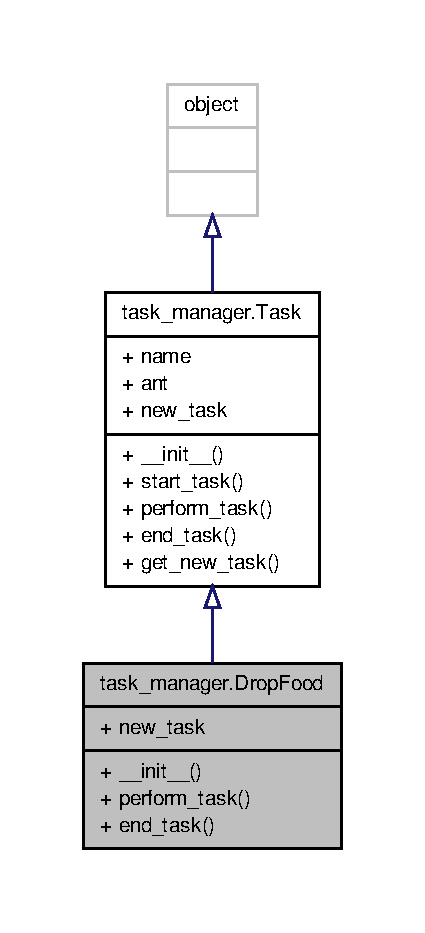
\includegraphics[width=204pt]{classtask__manager_1_1DropFood__inherit__graph}
\end{center}
\end{figure}


Collaboration diagram for task\+\_\+manager.\+Drop\+Food\+:\nopagebreak
\begin{figure}[H]
\begin{center}
\leavevmode
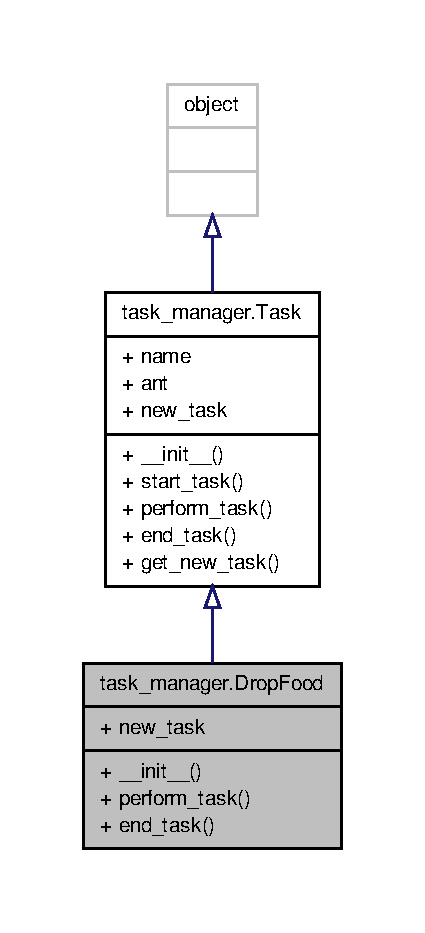
\includegraphics[width=204pt]{classtask__manager_1_1DropFood__coll__graph}
\end{center}
\end{figure}
\subsection*{Public Member Functions}
\begin{DoxyCompactItemize}
\item 
def \hyperlink{classtask__manager_1_1DropFood_a0f759e307357de441edd8465313ca4e8}{\+\_\+\+\_\+init\+\_\+\+\_\+}
\item 
def \hyperlink{classtask__manager_1_1DropFood_a82661a2394895191b28bb7ac1aeb5bf4}{perform\+\_\+task}
\item 
def \hyperlink{classtask__manager_1_1DropFood_aedccf366d55d4b081239ff27b72d896d}{end\+\_\+task}
\end{DoxyCompactItemize}
\subsection*{Public Attributes}
\begin{DoxyCompactItemize}
\item 
\hyperlink{classtask__manager_1_1DropFood_a9c3891af721254b73254732f0cb18f59}{new\+\_\+task}
\end{DoxyCompactItemize}


\subsection{Detailed Description}
\begin{DoxyVerb}Drop Food Task\end{DoxyVerb}
 

Definition at line \hyperlink{task__manager_8py_source_l00126}{126} of file \hyperlink{task__manager_8py_source}{task\+\_\+manager.\+py}.



\subsection{Constructor \& Destructor Documentation}
\hypertarget{classtask__manager_1_1DropFood_a0f759e307357de441edd8465313ca4e8}{\index{task\+\_\+manager\+::\+Drop\+Food@{task\+\_\+manager\+::\+Drop\+Food}!\+\_\+\+\_\+init\+\_\+\+\_\+@{\+\_\+\+\_\+init\+\_\+\+\_\+}}
\index{\+\_\+\+\_\+init\+\_\+\+\_\+@{\+\_\+\+\_\+init\+\_\+\+\_\+}!task\+\_\+manager\+::\+Drop\+Food@{task\+\_\+manager\+::\+Drop\+Food}}
\subsubsection[{\+\_\+\+\_\+init\+\_\+\+\_\+}]{\setlength{\rightskip}{0pt plus 5cm}def task\+\_\+manager.\+Drop\+Food.\+\_\+\+\_\+init\+\_\+\+\_\+ (
\begin{DoxyParamCaption}
\item[{}]{self, }
\item[{}]{ant}
\end{DoxyParamCaption}
)}}\label{classtask__manager_1_1DropFood_a0f759e307357de441edd8465313ca4e8}


Definition at line \hyperlink{task__manager_8py_source_l00128}{128} of file \hyperlink{task__manager_8py_source}{task\+\_\+manager.\+py}.



\subsection{Member Function Documentation}
\hypertarget{classtask__manager_1_1DropFood_aedccf366d55d4b081239ff27b72d896d}{\index{task\+\_\+manager\+::\+Drop\+Food@{task\+\_\+manager\+::\+Drop\+Food}!end\+\_\+task@{end\+\_\+task}}
\index{end\+\_\+task@{end\+\_\+task}!task\+\_\+manager\+::\+Drop\+Food@{task\+\_\+manager\+::\+Drop\+Food}}
\subsubsection[{end\+\_\+task}]{\setlength{\rightskip}{0pt plus 5cm}def task\+\_\+manager.\+Drop\+Food.\+end\+\_\+task (
\begin{DoxyParamCaption}
\item[{}]{self}
\end{DoxyParamCaption}
)}}\label{classtask__manager_1_1DropFood_aedccf366d55d4b081239ff27b72d896d}
\begin{DoxyVerb}Increase home scent strength and reduce food scent strength
\end{DoxyVerb}
 

Definition at line \hyperlink{task__manager_8py_source_l00146}{146} of file \hyperlink{task__manager_8py_source}{task\+\_\+manager.\+py}.

\hypertarget{classtask__manager_1_1DropFood_a82661a2394895191b28bb7ac1aeb5bf4}{\index{task\+\_\+manager\+::\+Drop\+Food@{task\+\_\+manager\+::\+Drop\+Food}!perform\+\_\+task@{perform\+\_\+task}}
\index{perform\+\_\+task@{perform\+\_\+task}!task\+\_\+manager\+::\+Drop\+Food@{task\+\_\+manager\+::\+Drop\+Food}}
\subsubsection[{perform\+\_\+task}]{\setlength{\rightskip}{0pt plus 5cm}def task\+\_\+manager.\+Drop\+Food.\+perform\+\_\+task (
\begin{DoxyParamCaption}
\item[{}]{self}
\end{DoxyParamCaption}
)}}\label{classtask__manager_1_1DropFood_a82661a2394895191b28bb7ac1aeb5bf4}
\begin{DoxyVerb}If ant reaches home drop the food inside the home
otherwise follow a home trail
\end{DoxyVerb}
 

Definition at line \hyperlink{task__manager_8py_source_l00131}{131} of file \hyperlink{task__manager_8py_source}{task\+\_\+manager.\+py}.



\subsection{Member Data Documentation}
\hypertarget{classtask__manager_1_1DropFood_a9c3891af721254b73254732f0cb18f59}{\index{task\+\_\+manager\+::\+Drop\+Food@{task\+\_\+manager\+::\+Drop\+Food}!new\+\_\+task@{new\+\_\+task}}
\index{new\+\_\+task@{new\+\_\+task}!task\+\_\+manager\+::\+Drop\+Food@{task\+\_\+manager\+::\+Drop\+Food}}
\subsubsection[{new\+\_\+task}]{\setlength{\rightskip}{0pt plus 5cm}task\+\_\+manager.\+Drop\+Food.\+new\+\_\+task}}\label{classtask__manager_1_1DropFood_a9c3891af721254b73254732f0cb18f59}


Definition at line \hyperlink{task__manager_8py_source_l00142}{142} of file \hyperlink{task__manager_8py_source}{task\+\_\+manager.\+py}.



The documentation for this class was generated from the following file\+:\begin{DoxyCompactItemize}
\item 
\hyperlink{task__manager_8py}{task\+\_\+manager.\+py}\end{DoxyCompactItemize}

\hypertarget{classdisplay_1_1Entity}{\section{display.\+Entity Class Reference}
\label{classdisplay_1_1Entity}\index{display.\+Entity@{display.\+Entity}}
}


Inheritance diagram for display.\+Entity\+:
\nopagebreak
\begin{figure}[H]
\begin{center}
\leavevmode
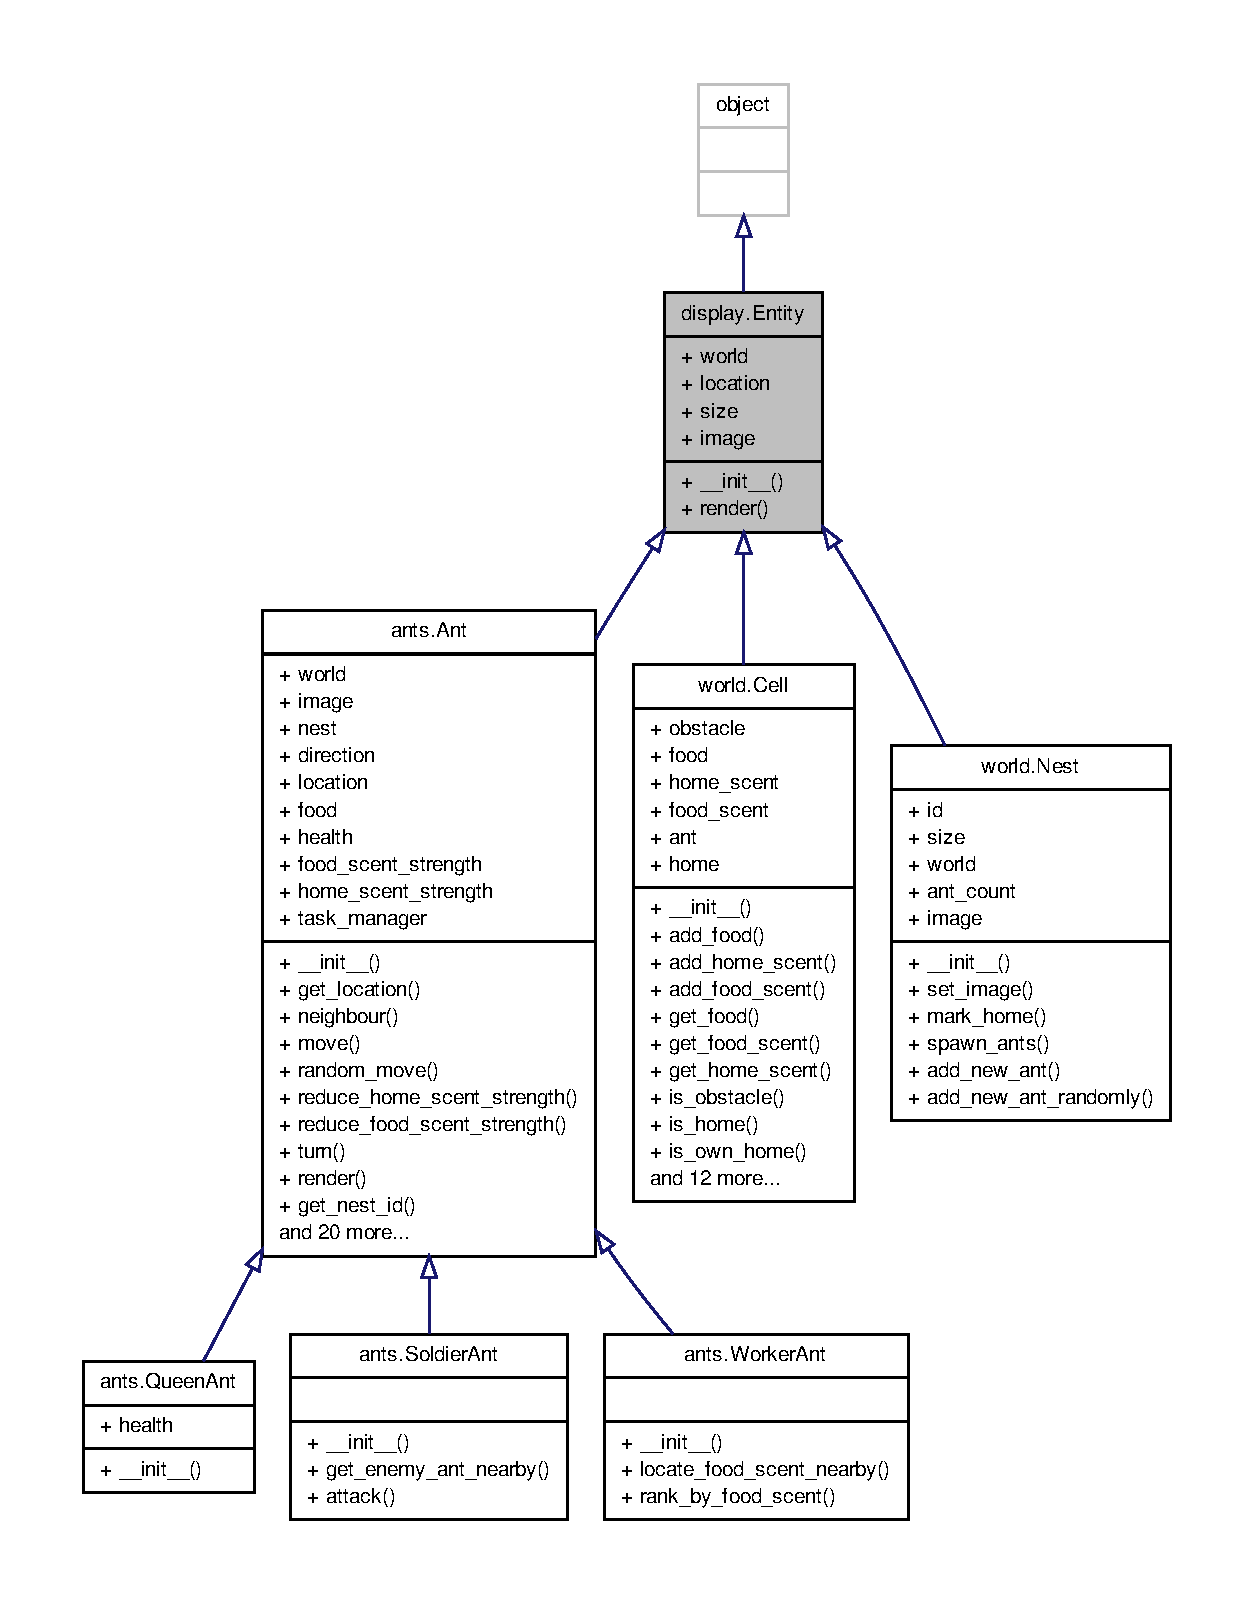
\includegraphics[width=350pt]{classdisplay_1_1Entity__inherit__graph}
\end{center}
\end{figure}


Collaboration diagram for display.\+Entity\+:\nopagebreak
\begin{figure}[H]
\begin{center}
\leavevmode
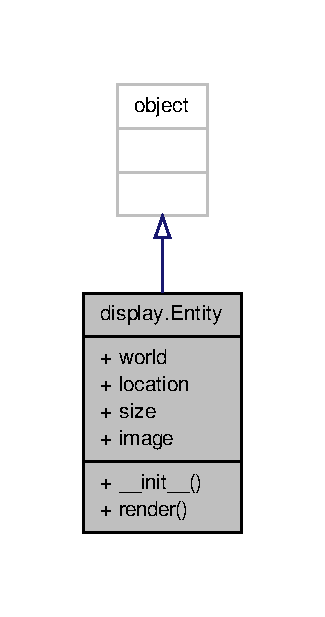
\includegraphics[width=156pt]{classdisplay_1_1Entity__coll__graph}
\end{center}
\end{figure}
\subsection*{Public Member Functions}
\begin{DoxyCompactItemize}
\item 
def \hyperlink{classdisplay_1_1Entity_a10294b5b8a8fa95f95f29aaf521efd56}{\+\_\+\+\_\+init\+\_\+\+\_\+}
\item 
def \hyperlink{classdisplay_1_1Entity_abbea5f77f08ce3347010d9c452440737}{render}
\end{DoxyCompactItemize}
\subsection*{Public Attributes}
\begin{DoxyCompactItemize}
\item 
\hyperlink{classdisplay_1_1Entity_ad7e3284bfb984c309b35d5a077bd5b21}{world}
\item 
\hyperlink{classdisplay_1_1Entity_ae2a1114b0c54ef7eb43c2bd6cd097258}{location}
\item 
\hyperlink{classdisplay_1_1Entity_aa56fd9b8bb6c9510f24ea13be8c6a218}{size}
\item 
\hyperlink{classdisplay_1_1Entity_a244569c285ad924e6200d4c1c8b4639c}{image}
\end{DoxyCompactItemize}


\subsection{Detailed Description}
\begin{DoxyVerb}Base class for all drawable objects
\end{DoxyVerb}
 

Definition at line \hyperlink{display_8py_source_l00001}{1} of file \hyperlink{display_8py_source}{display.\+py}.



\subsection{Constructor \& Destructor Documentation}
\hypertarget{classdisplay_1_1Entity_a10294b5b8a8fa95f95f29aaf521efd56}{\index{display\+::\+Entity@{display\+::\+Entity}!\+\_\+\+\_\+init\+\_\+\+\_\+@{\+\_\+\+\_\+init\+\_\+\+\_\+}}
\index{\+\_\+\+\_\+init\+\_\+\+\_\+@{\+\_\+\+\_\+init\+\_\+\+\_\+}!display\+::\+Entity@{display\+::\+Entity}}
\subsubsection[{\+\_\+\+\_\+init\+\_\+\+\_\+}]{\setlength{\rightskip}{0pt plus 5cm}def display.\+Entity.\+\_\+\+\_\+init\+\_\+\+\_\+ (
\begin{DoxyParamCaption}
\item[{}]{self, }
\item[{}]{world, }
\item[{}]{location, }
\item[{}]{size, }
\item[{}]{image}
\end{DoxyParamCaption}
)}}\label{classdisplay_1_1Entity_a10294b5b8a8fa95f95f29aaf521efd56}


Definition at line \hyperlink{display_8py_source_l00005}{5} of file \hyperlink{display_8py_source}{display.\+py}.



\subsection{Member Function Documentation}
\hypertarget{classdisplay_1_1Entity_abbea5f77f08ce3347010d9c452440737}{\index{display\+::\+Entity@{display\+::\+Entity}!render@{render}}
\index{render@{render}!display\+::\+Entity@{display\+::\+Entity}}
\subsubsection[{render}]{\setlength{\rightskip}{0pt plus 5cm}def display.\+Entity.\+render (
\begin{DoxyParamCaption}
\item[{}]{self, }
\item[{}]{index = {\ttfamily 0}}
\end{DoxyParamCaption}
)}}\label{classdisplay_1_1Entity_abbea5f77f08ce3347010d9c452440737}
\begin{DoxyVerb}Draw the object into the screen
    - selects the portion of the image to draw from the "index" argument
\end{DoxyVerb}
 

Definition at line \hyperlink{display_8py_source_l00011}{11} of file \hyperlink{display_8py_source}{display.\+py}.



\subsection{Member Data Documentation}
\hypertarget{classdisplay_1_1Entity_a244569c285ad924e6200d4c1c8b4639c}{\index{display\+::\+Entity@{display\+::\+Entity}!image@{image}}
\index{image@{image}!display\+::\+Entity@{display\+::\+Entity}}
\subsubsection[{image}]{\setlength{\rightskip}{0pt plus 5cm}display.\+Entity.\+image}}\label{classdisplay_1_1Entity_a244569c285ad924e6200d4c1c8b4639c}


Definition at line \hyperlink{display_8py_source_l00009}{9} of file \hyperlink{display_8py_source}{display.\+py}.

\hypertarget{classdisplay_1_1Entity_ae2a1114b0c54ef7eb43c2bd6cd097258}{\index{display\+::\+Entity@{display\+::\+Entity}!location@{location}}
\index{location@{location}!display\+::\+Entity@{display\+::\+Entity}}
\subsubsection[{location}]{\setlength{\rightskip}{0pt plus 5cm}display.\+Entity.\+location}}\label{classdisplay_1_1Entity_ae2a1114b0c54ef7eb43c2bd6cd097258}


Definition at line \hyperlink{display_8py_source_l00007}{7} of file \hyperlink{display_8py_source}{display.\+py}.

\hypertarget{classdisplay_1_1Entity_aa56fd9b8bb6c9510f24ea13be8c6a218}{\index{display\+::\+Entity@{display\+::\+Entity}!size@{size}}
\index{size@{size}!display\+::\+Entity@{display\+::\+Entity}}
\subsubsection[{size}]{\setlength{\rightskip}{0pt plus 5cm}display.\+Entity.\+size}}\label{classdisplay_1_1Entity_aa56fd9b8bb6c9510f24ea13be8c6a218}


Definition at line \hyperlink{display_8py_source_l00008}{8} of file \hyperlink{display_8py_source}{display.\+py}.

\hypertarget{classdisplay_1_1Entity_ad7e3284bfb984c309b35d5a077bd5b21}{\index{display\+::\+Entity@{display\+::\+Entity}!world@{world}}
\index{world@{world}!display\+::\+Entity@{display\+::\+Entity}}
\subsubsection[{world}]{\setlength{\rightskip}{0pt plus 5cm}display.\+Entity.\+world}}\label{classdisplay_1_1Entity_ad7e3284bfb984c309b35d5a077bd5b21}


Definition at line \hyperlink{display_8py_source_l00006}{6} of file \hyperlink{display_8py_source}{display.\+py}.



The documentation for this class was generated from the following file\+:\begin{DoxyCompactItemize}
\item 
\hyperlink{display_8py}{display.\+py}\end{DoxyCompactItemize}

\hypertarget{classtask__manager_1_1Explore}{\section{task\+\_\+manager.\+Explore Class Reference}
\label{classtask__manager_1_1Explore}\index{task\+\_\+manager.\+Explore@{task\+\_\+manager.\+Explore}}
}


Inheritance diagram for task\+\_\+manager.\+Explore\+:
\nopagebreak
\begin{figure}[H]
\begin{center}
\leavevmode
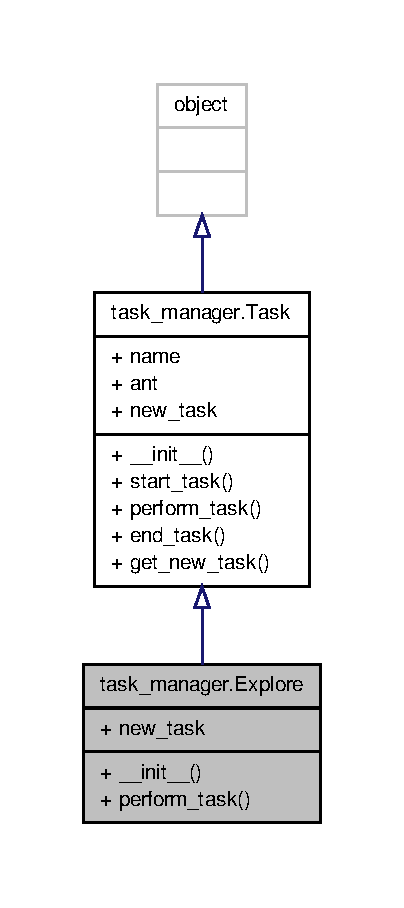
\includegraphics[width=194pt]{classtask__manager_1_1Explore__inherit__graph}
\end{center}
\end{figure}


Collaboration diagram for task\+\_\+manager.\+Explore\+:
\nopagebreak
\begin{figure}[H]
\begin{center}
\leavevmode
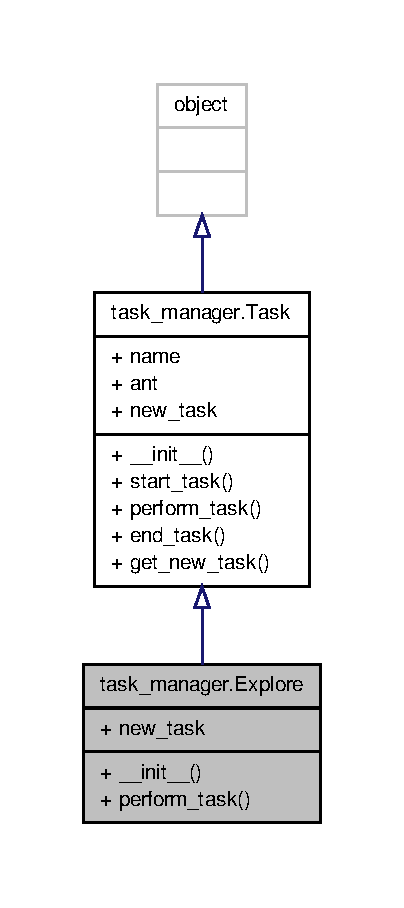
\includegraphics[width=194pt]{classtask__manager_1_1Explore__coll__graph}
\end{center}
\end{figure}
\subsection*{Public Member Functions}
\begin{DoxyCompactItemize}
\item 
def \hyperlink{classtask__manager_1_1Explore_ae95cc7a4676c07732fcf0faed752959c}{\+\_\+\+\_\+init\+\_\+\+\_\+}
\item 
def \hyperlink{classtask__manager_1_1Explore_a8ba5647950e170022bec93bc73c4a8de}{perform\+\_\+task}
\end{DoxyCompactItemize}
\subsection*{Public Attributes}
\begin{DoxyCompactItemize}
\item 
\hyperlink{classtask__manager_1_1Explore_ab1f83ac00c442f8eedd1403a59e74060}{new\+\_\+task}
\end{DoxyCompactItemize}


\subsection{Detailed Description}
\begin{DoxyVerb}Ant Exploring Task\end{DoxyVerb}
 

Definition at line \hyperlink{task__manager_8py_source_l00056}{56} of file \hyperlink{task__manager_8py_source}{task\+\_\+manager.\+py}.



\subsection{Constructor \& Destructor Documentation}
\hypertarget{classtask__manager_1_1Explore_ae95cc7a4676c07732fcf0faed752959c}{\index{task\+\_\+manager\+::\+Explore@{task\+\_\+manager\+::\+Explore}!\+\_\+\+\_\+init\+\_\+\+\_\+@{\+\_\+\+\_\+init\+\_\+\+\_\+}}
\index{\+\_\+\+\_\+init\+\_\+\+\_\+@{\+\_\+\+\_\+init\+\_\+\+\_\+}!task\+\_\+manager\+::\+Explore@{task\+\_\+manager\+::\+Explore}}
\subsubsection[{\+\_\+\+\_\+init\+\_\+\+\_\+}]{\setlength{\rightskip}{0pt plus 5cm}def task\+\_\+manager.\+Explore.\+\_\+\+\_\+init\+\_\+\+\_\+ (
\begin{DoxyParamCaption}
\item[{}]{self, }
\item[{}]{ant}
\end{DoxyParamCaption}
)}}\label{classtask__manager_1_1Explore_ae95cc7a4676c07732fcf0faed752959c}


Definition at line \hyperlink{task__manager_8py_source_l00058}{58} of file \hyperlink{task__manager_8py_source}{task\+\_\+manager.\+py}.



\subsection{Member Function Documentation}
\hypertarget{classtask__manager_1_1Explore_a8ba5647950e170022bec93bc73c4a8de}{\index{task\+\_\+manager\+::\+Explore@{task\+\_\+manager\+::\+Explore}!perform\+\_\+task@{perform\+\_\+task}}
\index{perform\+\_\+task@{perform\+\_\+task}!task\+\_\+manager\+::\+Explore@{task\+\_\+manager\+::\+Explore}}
\subsubsection[{perform\+\_\+task}]{\setlength{\rightskip}{0pt plus 5cm}def task\+\_\+manager.\+Explore.\+perform\+\_\+task (
\begin{DoxyParamCaption}
\item[{}]{self}
\end{DoxyParamCaption}
)}}\label{classtask__manager_1_1Explore_a8ba5647950e170022bec93bc73c4a8de}
\begin{DoxyVerb} If ant has food - 
     find home nearby and drop food there, else
     find home scent nearby and switch to that task, else
     make a random move
 If ant is searching for food
     if food is found switch to take food task, else
     find a food scent trail, else
     avoid obstacles
     reverse direction if it finds home nearby
 Reduce it scent strength by an unit
\end{DoxyVerb}
 

Definition at line \hyperlink{task__manager_8py_source_l00061}{61} of file \hyperlink{task__manager_8py_source}{task\+\_\+manager.\+py}.



\subsection{Member Data Documentation}
\hypertarget{classtask__manager_1_1Explore_ab1f83ac00c442f8eedd1403a59e74060}{\index{task\+\_\+manager\+::\+Explore@{task\+\_\+manager\+::\+Explore}!new\+\_\+task@{new\+\_\+task}}
\index{new\+\_\+task@{new\+\_\+task}!task\+\_\+manager\+::\+Explore@{task\+\_\+manager\+::\+Explore}}
\subsubsection[{new\+\_\+task}]{\setlength{\rightskip}{0pt plus 5cm}task\+\_\+manager.\+Explore.\+new\+\_\+task}}\label{classtask__manager_1_1Explore_ab1f83ac00c442f8eedd1403a59e74060}


Definition at line \hyperlink{task__manager_8py_source_l00079}{79} of file \hyperlink{task__manager_8py_source}{task\+\_\+manager.\+py}.



The documentation for this class was generated from the following file\+:\begin{DoxyCompactItemize}
\item 
\hyperlink{task__manager_8py}{task\+\_\+manager.\+py}\end{DoxyCompactItemize}

\hypertarget{classtask__manager_1_1FindFood}{\section{task\+\_\+manager.\+Find\+Food Class Reference}
\label{classtask__manager_1_1FindFood}\index{task\+\_\+manager.\+Find\+Food@{task\+\_\+manager.\+Find\+Food}}
}


Inheritance diagram for task\+\_\+manager.\+Find\+Food\+:
\nopagebreak
\begin{figure}[H]
\begin{center}
\leavevmode
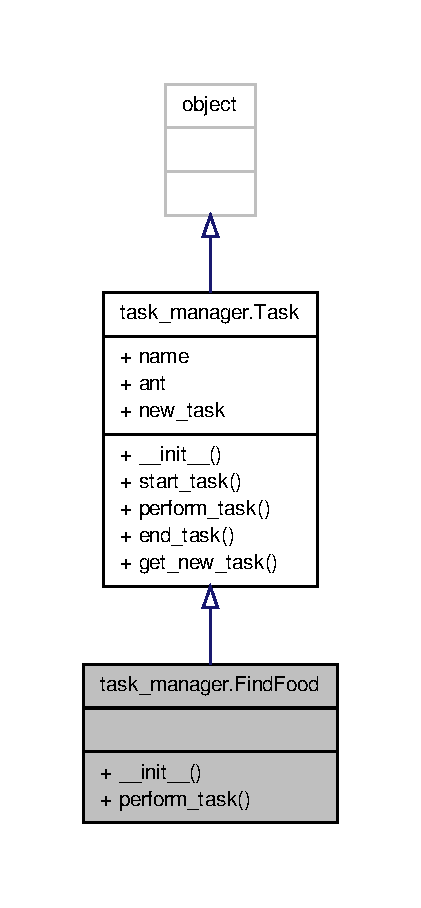
\includegraphics[width=202pt]{classtask__manager_1_1FindFood__inherit__graph}
\end{center}
\end{figure}


Collaboration diagram for task\+\_\+manager.\+Find\+Food\+:
\nopagebreak
\begin{figure}[H]
\begin{center}
\leavevmode
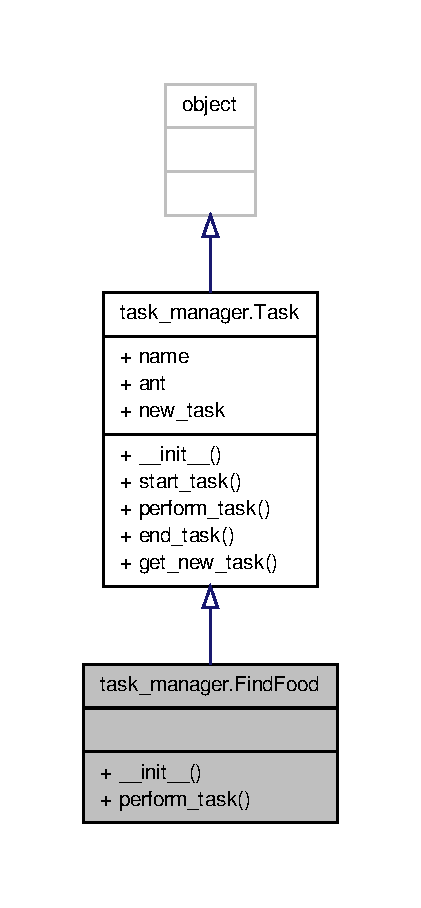
\includegraphics[width=202pt]{classtask__manager_1_1FindFood__coll__graph}
\end{center}
\end{figure}
\subsection*{Public Member Functions}
\begin{DoxyCompactItemize}
\item 
def \hyperlink{classtask__manager_1_1FindFood_abf53da166a9a36fbab4ce1c87fa93694}{\+\_\+\+\_\+init\+\_\+\+\_\+}
\item 
def \hyperlink{classtask__manager_1_1FindFood_aab9303f02e5e7d4884228e1fe5f6142c}{perform\+\_\+task}
\end{DoxyCompactItemize}
\subsection*{Additional Inherited Members}


\subsection{Detailed Description}
\begin{DoxyVerb}Finds food if hungry\end{DoxyVerb}
 

Definition at line \hyperlink{task__manager_8py_source_l00337}{337} of file \hyperlink{task__manager_8py_source}{task\+\_\+manager.\+py}.



\subsection{Constructor \& Destructor Documentation}
\hypertarget{classtask__manager_1_1FindFood_abf53da166a9a36fbab4ce1c87fa93694}{\index{task\+\_\+manager\+::\+Find\+Food@{task\+\_\+manager\+::\+Find\+Food}!\+\_\+\+\_\+init\+\_\+\+\_\+@{\+\_\+\+\_\+init\+\_\+\+\_\+}}
\index{\+\_\+\+\_\+init\+\_\+\+\_\+@{\+\_\+\+\_\+init\+\_\+\+\_\+}!task\+\_\+manager\+::\+Find\+Food@{task\+\_\+manager\+::\+Find\+Food}}
\subsubsection[{\+\_\+\+\_\+init\+\_\+\+\_\+}]{\setlength{\rightskip}{0pt plus 5cm}def task\+\_\+manager.\+Find\+Food.\+\_\+\+\_\+init\+\_\+\+\_\+ (
\begin{DoxyParamCaption}
\item[{}]{self, }
\item[{}]{ant}
\end{DoxyParamCaption}
)}}\label{classtask__manager_1_1FindFood_abf53da166a9a36fbab4ce1c87fa93694}


Definition at line \hyperlink{task__manager_8py_source_l00339}{339} of file \hyperlink{task__manager_8py_source}{task\+\_\+manager.\+py}.



\subsection{Member Function Documentation}
\hypertarget{classtask__manager_1_1FindFood_aab9303f02e5e7d4884228e1fe5f6142c}{\index{task\+\_\+manager\+::\+Find\+Food@{task\+\_\+manager\+::\+Find\+Food}!perform\+\_\+task@{perform\+\_\+task}}
\index{perform\+\_\+task@{perform\+\_\+task}!task\+\_\+manager\+::\+Find\+Food@{task\+\_\+manager\+::\+Find\+Food}}
\subsubsection[{perform\+\_\+task}]{\setlength{\rightskip}{0pt plus 5cm}def task\+\_\+manager.\+Find\+Food.\+perform\+\_\+task (
\begin{DoxyParamCaption}
\item[{}]{self}
\end{DoxyParamCaption}
)}}\label{classtask__manager_1_1FindFood_aab9303f02e5e7d4884228e1fe5f6142c}
\begin{DoxyVerb}find food\end{DoxyVerb}
 

Definition at line \hyperlink{task__manager_8py_source_l00342}{342} of file \hyperlink{task__manager_8py_source}{task\+\_\+manager.\+py}.



The documentation for this class was generated from the following file\+:\begin{DoxyCompactItemize}
\item 
\hyperlink{task__manager_8py}{task\+\_\+manager.\+py}\end{DoxyCompactItemize}

\hypertarget{classtask__manager_1_1FollowFoodTrail}{\section{task\+\_\+manager.\+Follow\+Food\+Trail Class Reference}
\label{classtask__manager_1_1FollowFoodTrail}\index{task\+\_\+manager.\+Follow\+Food\+Trail@{task\+\_\+manager.\+Follow\+Food\+Trail}}
}


Inheritance diagram for task\+\_\+manager.\+Follow\+Food\+Trail\+:\nopagebreak
\begin{figure}[H]
\begin{center}
\leavevmode
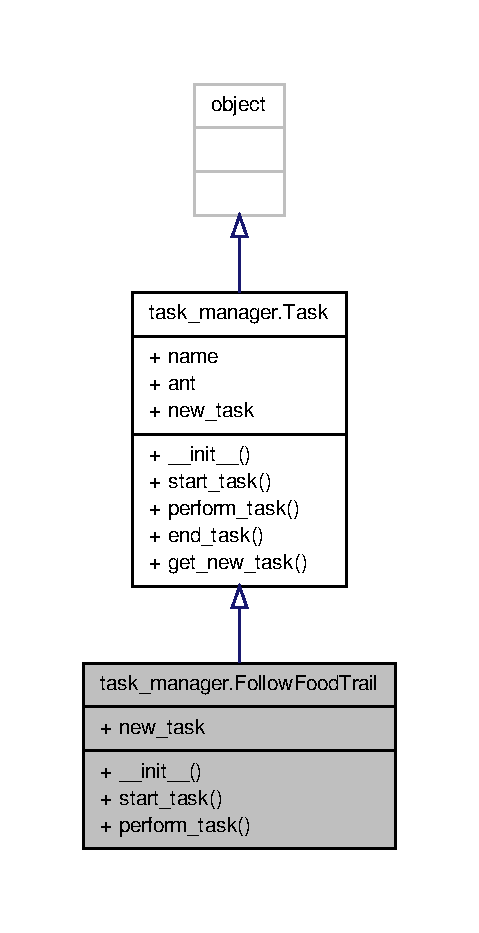
\includegraphics[width=230pt]{classtask__manager_1_1FollowFoodTrail__inherit__graph}
\end{center}
\end{figure}


Collaboration diagram for task\+\_\+manager.\+Follow\+Food\+Trail\+:\nopagebreak
\begin{figure}[H]
\begin{center}
\leavevmode
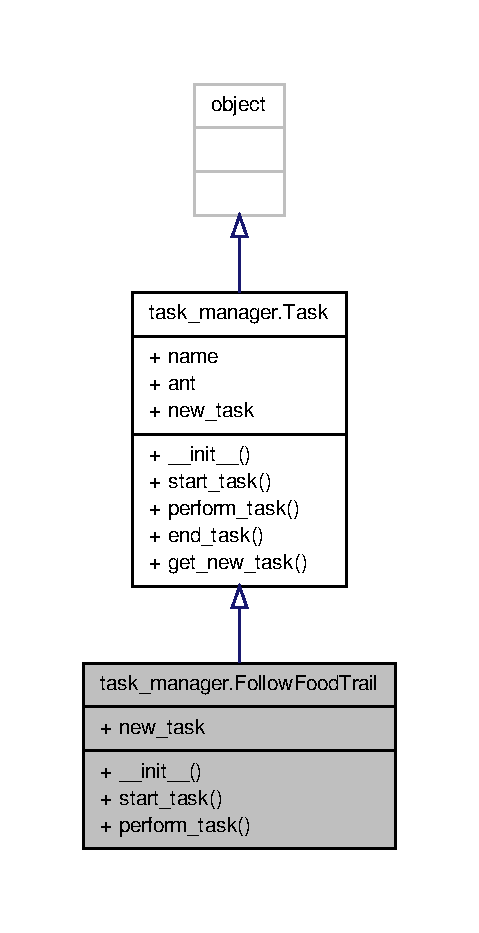
\includegraphics[width=230pt]{classtask__manager_1_1FollowFoodTrail__coll__graph}
\end{center}
\end{figure}
\subsection*{Public Member Functions}
\begin{DoxyCompactItemize}
\item 
def \hyperlink{classtask__manager_1_1FollowFoodTrail_a6af05bfd09141281c9943c8f01a0896b}{\+\_\+\+\_\+init\+\_\+\+\_\+}
\item 
def \hyperlink{classtask__manager_1_1FollowFoodTrail_a68013dbb3ab9d25676217de4d22c48eb}{start\+\_\+task}
\item 
def \hyperlink{classtask__manager_1_1FollowFoodTrail_aa805a2a4e9a76ba7afa252ca5efbd121}{perform\+\_\+task}
\end{DoxyCompactItemize}
\subsection*{Public Attributes}
\begin{DoxyCompactItemize}
\item 
\hyperlink{classtask__manager_1_1FollowFoodTrail_aefc8c49492622a4e4fa61279fd52ed12}{new\+\_\+task}
\end{DoxyCompactItemize}


\subsection{Detailed Description}
\begin{DoxyVerb}docstring for FollowFoodTrail\end{DoxyVerb}
 

Definition at line \hyperlink{task__manager_8py_source_l00153}{153} of file \hyperlink{task__manager_8py_source}{task\+\_\+manager.\+py}.



\subsection{Constructor \& Destructor Documentation}
\hypertarget{classtask__manager_1_1FollowFoodTrail_a6af05bfd09141281c9943c8f01a0896b}{\index{task\+\_\+manager\+::\+Follow\+Food\+Trail@{task\+\_\+manager\+::\+Follow\+Food\+Trail}!\+\_\+\+\_\+init\+\_\+\+\_\+@{\+\_\+\+\_\+init\+\_\+\+\_\+}}
\index{\+\_\+\+\_\+init\+\_\+\+\_\+@{\+\_\+\+\_\+init\+\_\+\+\_\+}!task\+\_\+manager\+::\+Follow\+Food\+Trail@{task\+\_\+manager\+::\+Follow\+Food\+Trail}}
\subsubsection[{\+\_\+\+\_\+init\+\_\+\+\_\+}]{\setlength{\rightskip}{0pt plus 5cm}def task\+\_\+manager.\+Follow\+Food\+Trail.\+\_\+\+\_\+init\+\_\+\+\_\+ (
\begin{DoxyParamCaption}
\item[{}]{self, }
\item[{}]{ant}
\end{DoxyParamCaption}
)}}\label{classtask__manager_1_1FollowFoodTrail_a6af05bfd09141281c9943c8f01a0896b}


Definition at line \hyperlink{task__manager_8py_source_l00155}{155} of file \hyperlink{task__manager_8py_source}{task\+\_\+manager.\+py}.



\subsection{Member Function Documentation}
\hypertarget{classtask__manager_1_1FollowFoodTrail_aa805a2a4e9a76ba7afa252ca5efbd121}{\index{task\+\_\+manager\+::\+Follow\+Food\+Trail@{task\+\_\+manager\+::\+Follow\+Food\+Trail}!perform\+\_\+task@{perform\+\_\+task}}
\index{perform\+\_\+task@{perform\+\_\+task}!task\+\_\+manager\+::\+Follow\+Food\+Trail@{task\+\_\+manager\+::\+Follow\+Food\+Trail}}
\subsubsection[{perform\+\_\+task}]{\setlength{\rightskip}{0pt plus 5cm}def task\+\_\+manager.\+Follow\+Food\+Trail.\+perform\+\_\+task (
\begin{DoxyParamCaption}
\item[{}]{self}
\end{DoxyParamCaption}
)}}\label{classtask__manager_1_1FollowFoodTrail_aa805a2a4e9a76ba7afa252ca5efbd121}
\begin{DoxyVerb}if food is found take food_scent_strength
otherwise rank cells based on scent and follow it
if scent trail is lost, return to explore mode
\end{DoxyVerb}
 

Definition at line \hyperlink{task__manager_8py_source_l00161}{161} of file \hyperlink{task__manager_8py_source}{task\+\_\+manager.\+py}.

\hypertarget{classtask__manager_1_1FollowFoodTrail_a68013dbb3ab9d25676217de4d22c48eb}{\index{task\+\_\+manager\+::\+Follow\+Food\+Trail@{task\+\_\+manager\+::\+Follow\+Food\+Trail}!start\+\_\+task@{start\+\_\+task}}
\index{start\+\_\+task@{start\+\_\+task}!task\+\_\+manager\+::\+Follow\+Food\+Trail@{task\+\_\+manager\+::\+Follow\+Food\+Trail}}
\subsubsection[{start\+\_\+task}]{\setlength{\rightskip}{0pt plus 5cm}def task\+\_\+manager.\+Follow\+Food\+Trail.\+start\+\_\+task (
\begin{DoxyParamCaption}
\item[{}]{self}
\end{DoxyParamCaption}
)}}\label{classtask__manager_1_1FollowFoodTrail_a68013dbb3ab9d25676217de4d22c48eb}


Definition at line \hyperlink{task__manager_8py_source_l00158}{158} of file \hyperlink{task__manager_8py_source}{task\+\_\+manager.\+py}.



\subsection{Member Data Documentation}
\hypertarget{classtask__manager_1_1FollowFoodTrail_aefc8c49492622a4e4fa61279fd52ed12}{\index{task\+\_\+manager\+::\+Follow\+Food\+Trail@{task\+\_\+manager\+::\+Follow\+Food\+Trail}!new\+\_\+task@{new\+\_\+task}}
\index{new\+\_\+task@{new\+\_\+task}!task\+\_\+manager\+::\+Follow\+Food\+Trail@{task\+\_\+manager\+::\+Follow\+Food\+Trail}}
\subsubsection[{new\+\_\+task}]{\setlength{\rightskip}{0pt plus 5cm}task\+\_\+manager.\+Follow\+Food\+Trail.\+new\+\_\+task}}\label{classtask__manager_1_1FollowFoodTrail_aefc8c49492622a4e4fa61279fd52ed12}


Definition at line \hyperlink{task__manager_8py_source_l00172}{172} of file \hyperlink{task__manager_8py_source}{task\+\_\+manager.\+py}.



The documentation for this class was generated from the following file\+:\begin{DoxyCompactItemize}
\item 
\hyperlink{task__manager_8py}{task\+\_\+manager.\+py}\end{DoxyCompactItemize}

\hypertarget{classtask__manager_1_1FollowHomeTrail}{\section{task\+\_\+manager.\+Follow\+Home\+Trail Class Reference}
\label{classtask__manager_1_1FollowHomeTrail}\index{task\+\_\+manager.\+Follow\+Home\+Trail@{task\+\_\+manager.\+Follow\+Home\+Trail}}
}


Inheritance diagram for task\+\_\+manager.\+Follow\+Home\+Trail\+:\nopagebreak
\begin{figure}[H]
\begin{center}
\leavevmode
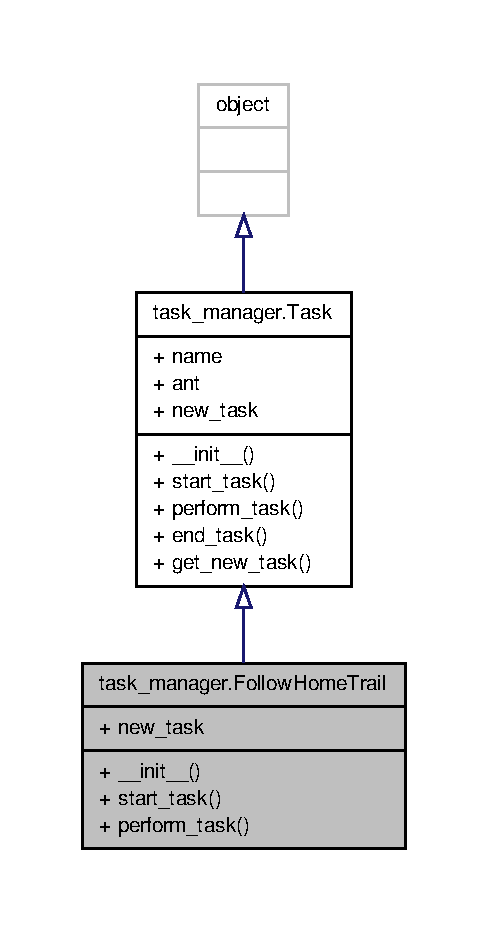
\includegraphics[width=234pt]{classtask__manager_1_1FollowHomeTrail__inherit__graph}
\end{center}
\end{figure}


Collaboration diagram for task\+\_\+manager.\+Follow\+Home\+Trail\+:\nopagebreak
\begin{figure}[H]
\begin{center}
\leavevmode
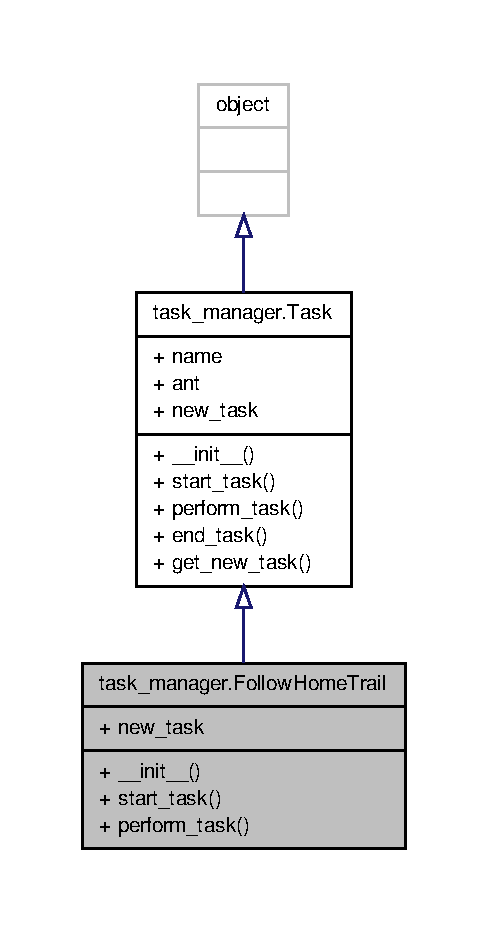
\includegraphics[width=234pt]{classtask__manager_1_1FollowHomeTrail__coll__graph}
\end{center}
\end{figure}
\subsection*{Public Member Functions}
\begin{DoxyCompactItemize}
\item 
def \hyperlink{classtask__manager_1_1FollowHomeTrail_a644c02e687f8a412a39e81628742f3b5}{\+\_\+\+\_\+init\+\_\+\+\_\+}
\item 
def \hyperlink{classtask__manager_1_1FollowHomeTrail_a0ffd4aabfafcfead05a02e149e5fab91}{start\+\_\+task}
\item 
def \hyperlink{classtask__manager_1_1FollowHomeTrail_ae4386ef7470e20e3f42fab9fc65b70cb}{perform\+\_\+task}
\end{DoxyCompactItemize}
\subsection*{Public Attributes}
\begin{DoxyCompactItemize}
\item 
\hyperlink{classtask__manager_1_1FollowHomeTrail_aae7878e14c1b1aeeac617e2e03074705}{new\+\_\+task}
\end{DoxyCompactItemize}


\subsection{Detailed Description}
\begin{DoxyVerb}Follows a home trail if it finds home scent 
\end{DoxyVerb}
 

Definition at line \hyperlink{task__manager_8py_source_l00223}{223} of file \hyperlink{task__manager_8py_source}{task\+\_\+manager.\+py}.



\subsection{Constructor \& Destructor Documentation}
\hypertarget{classtask__manager_1_1FollowHomeTrail_a644c02e687f8a412a39e81628742f3b5}{\index{task\+\_\+manager\+::\+Follow\+Home\+Trail@{task\+\_\+manager\+::\+Follow\+Home\+Trail}!\+\_\+\+\_\+init\+\_\+\+\_\+@{\+\_\+\+\_\+init\+\_\+\+\_\+}}
\index{\+\_\+\+\_\+init\+\_\+\+\_\+@{\+\_\+\+\_\+init\+\_\+\+\_\+}!task\+\_\+manager\+::\+Follow\+Home\+Trail@{task\+\_\+manager\+::\+Follow\+Home\+Trail}}
\subsubsection[{\+\_\+\+\_\+init\+\_\+\+\_\+}]{\setlength{\rightskip}{0pt plus 5cm}def task\+\_\+manager.\+Follow\+Home\+Trail.\+\_\+\+\_\+init\+\_\+\+\_\+ (
\begin{DoxyParamCaption}
\item[{}]{self, }
\item[{}]{ant}
\end{DoxyParamCaption}
)}}\label{classtask__manager_1_1FollowHomeTrail_a644c02e687f8a412a39e81628742f3b5}


Definition at line \hyperlink{task__manager_8py_source_l00227}{227} of file \hyperlink{task__manager_8py_source}{task\+\_\+manager.\+py}.



\subsection{Member Function Documentation}
\hypertarget{classtask__manager_1_1FollowHomeTrail_ae4386ef7470e20e3f42fab9fc65b70cb}{\index{task\+\_\+manager\+::\+Follow\+Home\+Trail@{task\+\_\+manager\+::\+Follow\+Home\+Trail}!perform\+\_\+task@{perform\+\_\+task}}
\index{perform\+\_\+task@{perform\+\_\+task}!task\+\_\+manager\+::\+Follow\+Home\+Trail@{task\+\_\+manager\+::\+Follow\+Home\+Trail}}
\subsubsection[{perform\+\_\+task}]{\setlength{\rightskip}{0pt plus 5cm}def task\+\_\+manager.\+Follow\+Home\+Trail.\+perform\+\_\+task (
\begin{DoxyParamCaption}
\item[{}]{self}
\end{DoxyParamCaption}
)}}\label{classtask__manager_1_1FollowHomeTrail_ae4386ef7470e20e3f42fab9fc65b70cb}
\begin{DoxyVerb}    If home is reached drop the food_scent_strength
    If trail is lost return to explore mode
    else rank the cell by home scent strength and follow itself
\end{DoxyVerb}
 

Definition at line \hyperlink{task__manager_8py_source_l00233}{233} of file \hyperlink{task__manager_8py_source}{task\+\_\+manager.\+py}.

\hypertarget{classtask__manager_1_1FollowHomeTrail_a0ffd4aabfafcfead05a02e149e5fab91}{\index{task\+\_\+manager\+::\+Follow\+Home\+Trail@{task\+\_\+manager\+::\+Follow\+Home\+Trail}!start\+\_\+task@{start\+\_\+task}}
\index{start\+\_\+task@{start\+\_\+task}!task\+\_\+manager\+::\+Follow\+Home\+Trail@{task\+\_\+manager\+::\+Follow\+Home\+Trail}}
\subsubsection[{start\+\_\+task}]{\setlength{\rightskip}{0pt plus 5cm}def task\+\_\+manager.\+Follow\+Home\+Trail.\+start\+\_\+task (
\begin{DoxyParamCaption}
\item[{}]{self}
\end{DoxyParamCaption}
)}}\label{classtask__manager_1_1FollowHomeTrail_a0ffd4aabfafcfead05a02e149e5fab91}


Definition at line \hyperlink{task__manager_8py_source_l00230}{230} of file \hyperlink{task__manager_8py_source}{task\+\_\+manager.\+py}.



\subsection{Member Data Documentation}
\hypertarget{classtask__manager_1_1FollowHomeTrail_aae7878e14c1b1aeeac617e2e03074705}{\index{task\+\_\+manager\+::\+Follow\+Home\+Trail@{task\+\_\+manager\+::\+Follow\+Home\+Trail}!new\+\_\+task@{new\+\_\+task}}
\index{new\+\_\+task@{new\+\_\+task}!task\+\_\+manager\+::\+Follow\+Home\+Trail@{task\+\_\+manager\+::\+Follow\+Home\+Trail}}
\subsubsection[{new\+\_\+task}]{\setlength{\rightskip}{0pt plus 5cm}task\+\_\+manager.\+Follow\+Home\+Trail.\+new\+\_\+task}}\label{classtask__manager_1_1FollowHomeTrail_aae7878e14c1b1aeeac617e2e03074705}


Definition at line \hyperlink{task__manager_8py_source_l00242}{242} of file \hyperlink{task__manager_8py_source}{task\+\_\+manager.\+py}.



The documentation for this class was generated from the following file\+:\begin{DoxyCompactItemize}
\item 
\hyperlink{task__manager_8py}{task\+\_\+manager.\+py}\end{DoxyCompactItemize}

\hypertarget{classtask__manager_1_1GuardNest}{\section{task\+\_\+manager.\+Guard\+Nest Class Reference}
\label{classtask__manager_1_1GuardNest}\index{task\+\_\+manager.\+Guard\+Nest@{task\+\_\+manager.\+Guard\+Nest}}
}


Inheritance diagram for task\+\_\+manager.\+Guard\+Nest\+:
\nopagebreak
\begin{figure}[H]
\begin{center}
\leavevmode
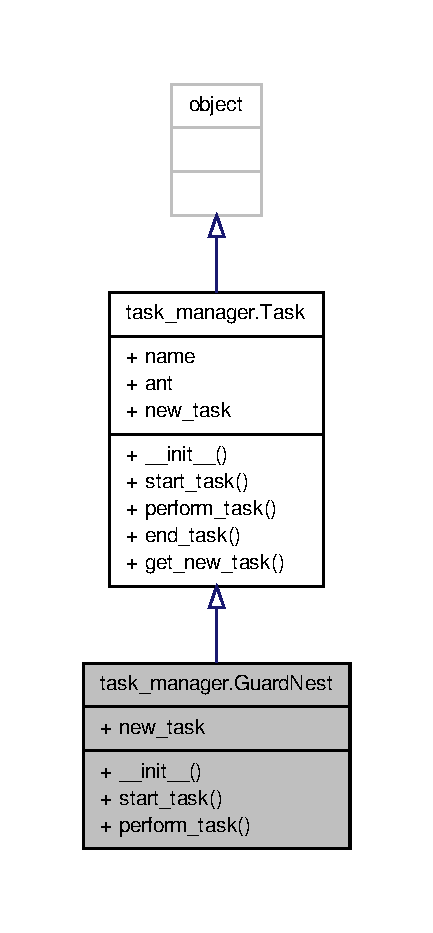
\includegraphics[width=208pt]{classtask__manager_1_1GuardNest__inherit__graph}
\end{center}
\end{figure}


Collaboration diagram for task\+\_\+manager.\+Guard\+Nest\+:
\nopagebreak
\begin{figure}[H]
\begin{center}
\leavevmode
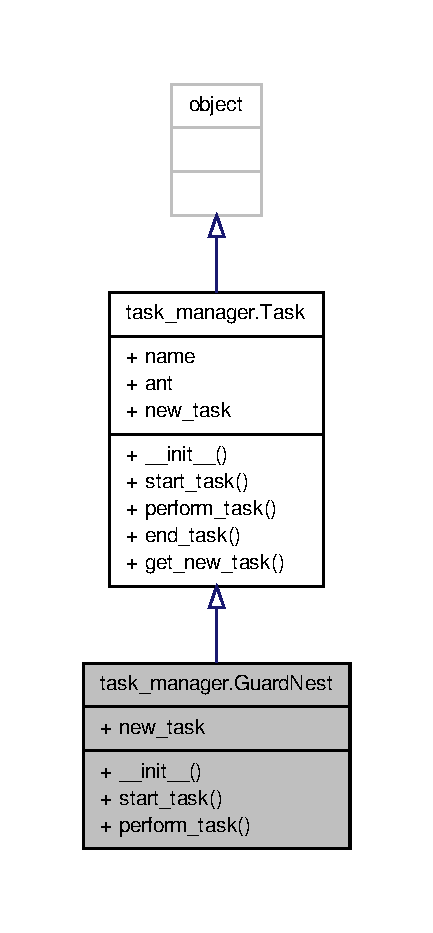
\includegraphics[width=208pt]{classtask__manager_1_1GuardNest__coll__graph}
\end{center}
\end{figure}
\subsection*{Public Member Functions}
\begin{DoxyCompactItemize}
\item 
def \hyperlink{classtask__manager_1_1GuardNest_ac1b98762825c860890caff5649269cb1}{\+\_\+\+\_\+init\+\_\+\+\_\+}
\item 
def \hyperlink{classtask__manager_1_1GuardNest_a44493cf7d0653d2b548040a5857ef330}{start\+\_\+task}
\item 
def \hyperlink{classtask__manager_1_1GuardNest_a18003edc3f1e2fca7bfe34cf078e96f8}{perform\+\_\+task}
\end{DoxyCompactItemize}
\subsection*{Public Attributes}
\begin{DoxyCompactItemize}
\item 
\hyperlink{classtask__manager_1_1GuardNest_ada22ecced047079d5f4d98a0b86a2d0e}{new\+\_\+task}
\end{DoxyCompactItemize}


\subsection{Detailed Description}
\begin{DoxyVerb}Guards the nest
If it sees an enemy ant it attacks it
\end{DoxyVerb}
 

Definition at line \hyperlink{task__manager_8py_source_l00293}{293} of file \hyperlink{task__manager_8py_source}{task\+\_\+manager.\+py}.



\subsection{Constructor \& Destructor Documentation}
\hypertarget{classtask__manager_1_1GuardNest_ac1b98762825c860890caff5649269cb1}{\index{task\+\_\+manager\+::\+Guard\+Nest@{task\+\_\+manager\+::\+Guard\+Nest}!\+\_\+\+\_\+init\+\_\+\+\_\+@{\+\_\+\+\_\+init\+\_\+\+\_\+}}
\index{\+\_\+\+\_\+init\+\_\+\+\_\+@{\+\_\+\+\_\+init\+\_\+\+\_\+}!task\+\_\+manager\+::\+Guard\+Nest@{task\+\_\+manager\+::\+Guard\+Nest}}
\subsubsection[{\+\_\+\+\_\+init\+\_\+\+\_\+}]{\setlength{\rightskip}{0pt plus 5cm}def task\+\_\+manager.\+Guard\+Nest.\+\_\+\+\_\+init\+\_\+\+\_\+ (
\begin{DoxyParamCaption}
\item[{}]{self, }
\item[{}]{ant}
\end{DoxyParamCaption}
)}}\label{classtask__manager_1_1GuardNest_ac1b98762825c860890caff5649269cb1}


Definition at line \hyperlink{task__manager_8py_source_l00298}{298} of file \hyperlink{task__manager_8py_source}{task\+\_\+manager.\+py}.



\subsection{Member Function Documentation}
\hypertarget{classtask__manager_1_1GuardNest_a18003edc3f1e2fca7bfe34cf078e96f8}{\index{task\+\_\+manager\+::\+Guard\+Nest@{task\+\_\+manager\+::\+Guard\+Nest}!perform\+\_\+task@{perform\+\_\+task}}
\index{perform\+\_\+task@{perform\+\_\+task}!task\+\_\+manager\+::\+Guard\+Nest@{task\+\_\+manager\+::\+Guard\+Nest}}
\subsubsection[{perform\+\_\+task}]{\setlength{\rightskip}{0pt plus 5cm}def task\+\_\+manager.\+Guard\+Nest.\+perform\+\_\+task (
\begin{DoxyParamCaption}
\item[{}]{self}
\end{DoxyParamCaption}
)}}\label{classtask__manager_1_1GuardNest_a18003edc3f1e2fca7bfe34cf078e96f8}
\begin{DoxyVerb}Travel along the walls of the nest
\end{DoxyVerb}
 

Definition at line \hyperlink{task__manager_8py_source_l00305}{305} of file \hyperlink{task__manager_8py_source}{task\+\_\+manager.\+py}.

\hypertarget{classtask__manager_1_1GuardNest_a44493cf7d0653d2b548040a5857ef330}{\index{task\+\_\+manager\+::\+Guard\+Nest@{task\+\_\+manager\+::\+Guard\+Nest}!start\+\_\+task@{start\+\_\+task}}
\index{start\+\_\+task@{start\+\_\+task}!task\+\_\+manager\+::\+Guard\+Nest@{task\+\_\+manager\+::\+Guard\+Nest}}
\subsubsection[{start\+\_\+task}]{\setlength{\rightskip}{0pt plus 5cm}def task\+\_\+manager.\+Guard\+Nest.\+start\+\_\+task (
\begin{DoxyParamCaption}
\item[{}]{self}
\end{DoxyParamCaption}
)}}\label{classtask__manager_1_1GuardNest_a44493cf7d0653d2b548040a5857ef330}


Definition at line \hyperlink{task__manager_8py_source_l00301}{301} of file \hyperlink{task__manager_8py_source}{task\+\_\+manager.\+py}.



\subsection{Member Data Documentation}
\hypertarget{classtask__manager_1_1GuardNest_ada22ecced047079d5f4d98a0b86a2d0e}{\index{task\+\_\+manager\+::\+Guard\+Nest@{task\+\_\+manager\+::\+Guard\+Nest}!new\+\_\+task@{new\+\_\+task}}
\index{new\+\_\+task@{new\+\_\+task}!task\+\_\+manager\+::\+Guard\+Nest@{task\+\_\+manager\+::\+Guard\+Nest}}
\subsubsection[{new\+\_\+task}]{\setlength{\rightskip}{0pt plus 5cm}task\+\_\+manager.\+Guard\+Nest.\+new\+\_\+task}}\label{classtask__manager_1_1GuardNest_ada22ecced047079d5f4d98a0b86a2d0e}


Definition at line \hyperlink{task__manager_8py_source_l00315}{315} of file \hyperlink{task__manager_8py_source}{task\+\_\+manager.\+py}.



The documentation for this class was generated from the following file\+:\begin{DoxyCompactItemize}
\item 
\hyperlink{task__manager_8py}{task\+\_\+manager.\+py}\end{DoxyCompactItemize}

\hypertarget{classworld_1_1Nest}{\section{world.\+Nest Class Reference}
\label{classworld_1_1Nest}\index{world.\+Nest@{world.\+Nest}}
}


Inheritance diagram for world.\+Nest\+:
\nopagebreak
\begin{figure}[H]
\begin{center}
\leavevmode
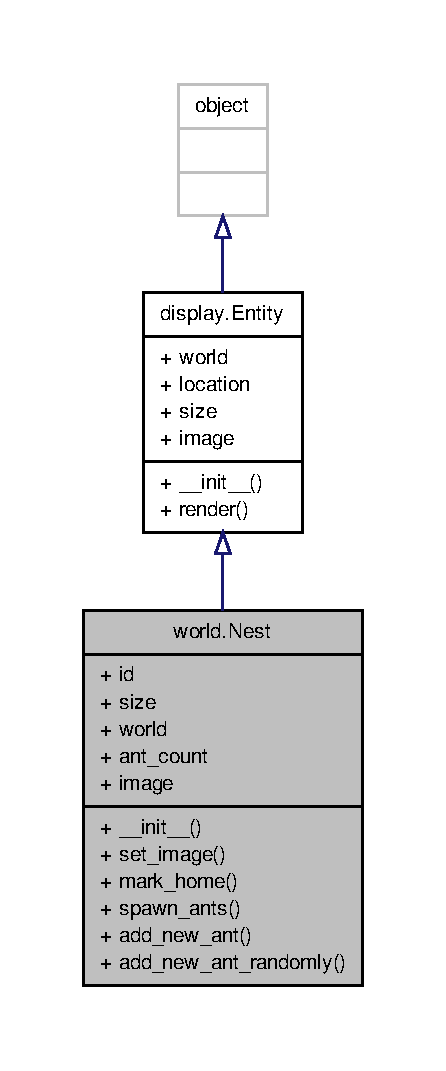
\includegraphics[width=214pt]{classworld_1_1Nest__inherit__graph}
\end{center}
\end{figure}


Collaboration diagram for world.\+Nest\+:
\nopagebreak
\begin{figure}[H]
\begin{center}
\leavevmode
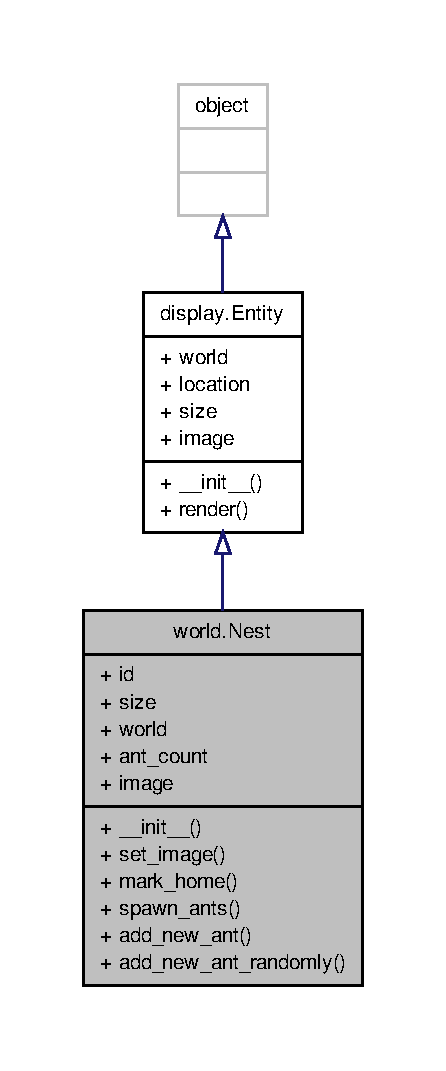
\includegraphics[width=214pt]{classworld_1_1Nest__coll__graph}
\end{center}
\end{figure}
\subsection*{Public Member Functions}
\begin{DoxyCompactItemize}
\item 
def \hyperlink{classworld_1_1Nest_a76e2fb1c7adfc7b4843bd9a1491c67f7}{\+\_\+\+\_\+init\+\_\+\+\_\+}
\item 
def \hyperlink{classworld_1_1Nest_a91914c56d2849f47dfd2b2ad97996fb6}{set\+\_\+image}
\item 
def \hyperlink{classworld_1_1Nest_a4a57d2cea404003ee77306758e9da3e1}{mark\+\_\+home}
\item 
def \hyperlink{classworld_1_1Nest_a756db917e2fa8aeb72c5277637822a53}{spawn\+\_\+ants}
\item 
def \hyperlink{classworld_1_1Nest_a0b76a02840f15fe7909859d523736a58}{add\+\_\+new\+\_\+ant}
\item 
def \hyperlink{classworld_1_1Nest_ac845bc370bbb778a45a360145a48be61}{add\+\_\+new\+\_\+ant\+\_\+randomly}
\end{DoxyCompactItemize}
\subsection*{Public Attributes}
\begin{DoxyCompactItemize}
\item 
\hyperlink{classworld_1_1Nest_a2ab2394f7ded6041e64cfea7390519c3}{id}
\item 
\hyperlink{classworld_1_1Nest_a779ec4ef0582e917964de4efaedaef84}{size}
\item 
\hyperlink{classworld_1_1Nest_a624fe0079926173a6356a3d59410dcf3}{world}
\item 
\hyperlink{classworld_1_1Nest_aa41cdaa8399fe934d89f5573ff804cbc}{ant\+\_\+count}
\item 
\hyperlink{classworld_1_1Nest_a1d943529c7685aa0cadeb43f9891ff03}{image}
\end{DoxyCompactItemize}


\subsection{Detailed Description}
\begin{DoxyVerb}Encapsulates a colony of ants
\end{DoxyVerb}
 

Definition at line \hyperlink{world_8py_source_l00213}{213} of file \hyperlink{world_8py_source}{world.\+py}.



\subsection{Constructor \& Destructor Documentation}
\hypertarget{classworld_1_1Nest_a76e2fb1c7adfc7b4843bd9a1491c67f7}{\index{world\+::\+Nest@{world\+::\+Nest}!\+\_\+\+\_\+init\+\_\+\+\_\+@{\+\_\+\+\_\+init\+\_\+\+\_\+}}
\index{\+\_\+\+\_\+init\+\_\+\+\_\+@{\+\_\+\+\_\+init\+\_\+\+\_\+}!world\+::\+Nest@{world\+::\+Nest}}
\subsubsection[{\+\_\+\+\_\+init\+\_\+\+\_\+}]{\setlength{\rightskip}{0pt plus 5cm}def world.\+Nest.\+\_\+\+\_\+init\+\_\+\+\_\+ (
\begin{DoxyParamCaption}
\item[{}]{self, }
\item[{}]{world, }
\item[{}]{id, }
\item[{}]{size, }
\item[{}]{location, }
\item[{}]{ant\+\_\+count}
\end{DoxyParamCaption}
)}}\label{classworld_1_1Nest_a76e2fb1c7adfc7b4843bd9a1491c67f7}


Definition at line \hyperlink{world_8py_source_l00217}{217} of file \hyperlink{world_8py_source}{world.\+py}.



\subsection{Member Function Documentation}
\hypertarget{classworld_1_1Nest_a0b76a02840f15fe7909859d523736a58}{\index{world\+::\+Nest@{world\+::\+Nest}!add\+\_\+new\+\_\+ant@{add\+\_\+new\+\_\+ant}}
\index{add\+\_\+new\+\_\+ant@{add\+\_\+new\+\_\+ant}!world\+::\+Nest@{world\+::\+Nest}}
\subsubsection[{add\+\_\+new\+\_\+ant}]{\setlength{\rightskip}{0pt plus 5cm}def world.\+Nest.\+add\+\_\+new\+\_\+ant (
\begin{DoxyParamCaption}
\item[{}]{self, }
\item[{}]{ant\+\_\+type}
\end{DoxyParamCaption}
)}}\label{classworld_1_1Nest_a0b76a02840f15fe7909859d523736a58}


Definition at line \hyperlink{world_8py_source_l00255}{255} of file \hyperlink{world_8py_source}{world.\+py}.

\hypertarget{classworld_1_1Nest_ac845bc370bbb778a45a360145a48be61}{\index{world\+::\+Nest@{world\+::\+Nest}!add\+\_\+new\+\_\+ant\+\_\+randomly@{add\+\_\+new\+\_\+ant\+\_\+randomly}}
\index{add\+\_\+new\+\_\+ant\+\_\+randomly@{add\+\_\+new\+\_\+ant\+\_\+randomly}!world\+::\+Nest@{world\+::\+Nest}}
\subsubsection[{add\+\_\+new\+\_\+ant\+\_\+randomly}]{\setlength{\rightskip}{0pt plus 5cm}def world.\+Nest.\+add\+\_\+new\+\_\+ant\+\_\+randomly (
\begin{DoxyParamCaption}
\item[{}]{self}
\end{DoxyParamCaption}
)}}\label{classworld_1_1Nest_ac845bc370bbb778a45a360145a48be61}


Definition at line \hyperlink{world_8py_source_l00263}{263} of file \hyperlink{world_8py_source}{world.\+py}.

\hypertarget{classworld_1_1Nest_a4a57d2cea404003ee77306758e9da3e1}{\index{world\+::\+Nest@{world\+::\+Nest}!mark\+\_\+home@{mark\+\_\+home}}
\index{mark\+\_\+home@{mark\+\_\+home}!world\+::\+Nest@{world\+::\+Nest}}
\subsubsection[{mark\+\_\+home}]{\setlength{\rightskip}{0pt plus 5cm}def world.\+Nest.\+mark\+\_\+home (
\begin{DoxyParamCaption}
\item[{}]{self}
\end{DoxyParamCaption}
)}}\label{classworld_1_1Nest_a4a57d2cea404003ee77306758e9da3e1}
\begin{DoxyVerb}Converts the cell at its location to its nest
\end{DoxyVerb}
 

Definition at line \hyperlink{world_8py_source_l00235}{235} of file \hyperlink{world_8py_source}{world.\+py}.

\hypertarget{classworld_1_1Nest_a91914c56d2849f47dfd2b2ad97996fb6}{\index{world\+::\+Nest@{world\+::\+Nest}!set\+\_\+image@{set\+\_\+image}}
\index{set\+\_\+image@{set\+\_\+image}!world\+::\+Nest@{world\+::\+Nest}}
\subsubsection[{set\+\_\+image}]{\setlength{\rightskip}{0pt plus 5cm}def world.\+Nest.\+set\+\_\+image (
\begin{DoxyParamCaption}
\item[{}]{self}
\end{DoxyParamCaption}
)}}\label{classworld_1_1Nest_a91914c56d2849f47dfd2b2ad97996fb6}


Definition at line \hyperlink{world_8py_source_l00227}{227} of file \hyperlink{world_8py_source}{world.\+py}.

\hypertarget{classworld_1_1Nest_a756db917e2fa8aeb72c5277637822a53}{\index{world\+::\+Nest@{world\+::\+Nest}!spawn\+\_\+ants@{spawn\+\_\+ants}}
\index{spawn\+\_\+ants@{spawn\+\_\+ants}!world\+::\+Nest@{world\+::\+Nest}}
\subsubsection[{spawn\+\_\+ants}]{\setlength{\rightskip}{0pt plus 5cm}def world.\+Nest.\+spawn\+\_\+ants (
\begin{DoxyParamCaption}
\item[{}]{self}
\end{DoxyParamCaption}
)}}\label{classworld_1_1Nest_a756db917e2fa8aeb72c5277637822a53}
\begin{DoxyVerb}Creates instances of ants and adds them into the world
\end{DoxyVerb}
 

Definition at line \hyperlink{world_8py_source_l00247}{247} of file \hyperlink{world_8py_source}{world.\+py}.



\subsection{Member Data Documentation}
\hypertarget{classworld_1_1Nest_aa41cdaa8399fe934d89f5573ff804cbc}{\index{world\+::\+Nest@{world\+::\+Nest}!ant\+\_\+count@{ant\+\_\+count}}
\index{ant\+\_\+count@{ant\+\_\+count}!world\+::\+Nest@{world\+::\+Nest}}
\subsubsection[{ant\+\_\+count}]{\setlength{\rightskip}{0pt plus 5cm}world.\+Nest.\+ant\+\_\+count}}\label{classworld_1_1Nest_aa41cdaa8399fe934d89f5573ff804cbc}


Definition at line \hyperlink{world_8py_source_l00221}{221} of file \hyperlink{world_8py_source}{world.\+py}.

\hypertarget{classworld_1_1Nest_a2ab2394f7ded6041e64cfea7390519c3}{\index{world\+::\+Nest@{world\+::\+Nest}!id@{id}}
\index{id@{id}!world\+::\+Nest@{world\+::\+Nest}}
\subsubsection[{id}]{\setlength{\rightskip}{0pt plus 5cm}world.\+Nest.\+id}}\label{classworld_1_1Nest_a2ab2394f7ded6041e64cfea7390519c3}


Definition at line \hyperlink{world_8py_source_l00218}{218} of file \hyperlink{world_8py_source}{world.\+py}.

\hypertarget{classworld_1_1Nest_a1d943529c7685aa0cadeb43f9891ff03}{\index{world\+::\+Nest@{world\+::\+Nest}!image@{image}}
\index{image@{image}!world\+::\+Nest@{world\+::\+Nest}}
\subsubsection[{image}]{\setlength{\rightskip}{0pt plus 5cm}world.\+Nest.\+image}}\label{classworld_1_1Nest_a1d943529c7685aa0cadeb43f9891ff03}


Definition at line \hyperlink{world_8py_source_l00231}{231} of file \hyperlink{world_8py_source}{world.\+py}.

\hypertarget{classworld_1_1Nest_a779ec4ef0582e917964de4efaedaef84}{\index{world\+::\+Nest@{world\+::\+Nest}!size@{size}}
\index{size@{size}!world\+::\+Nest@{world\+::\+Nest}}
\subsubsection[{size}]{\setlength{\rightskip}{0pt plus 5cm}world.\+Nest.\+size}}\label{classworld_1_1Nest_a779ec4ef0582e917964de4efaedaef84}


Definition at line \hyperlink{world_8py_source_l00219}{219} of file \hyperlink{world_8py_source}{world.\+py}.

\hypertarget{classworld_1_1Nest_a624fe0079926173a6356a3d59410dcf3}{\index{world\+::\+Nest@{world\+::\+Nest}!world@{world}}
\index{world@{world}!world\+::\+Nest@{world\+::\+Nest}}
\subsubsection[{world}]{\setlength{\rightskip}{0pt plus 5cm}world.\+Nest.\+world}}\label{classworld_1_1Nest_a624fe0079926173a6356a3d59410dcf3}


Definition at line \hyperlink{world_8py_source_l00220}{220} of file \hyperlink{world_8py_source}{world.\+py}.



The documentation for this class was generated from the following file\+:\begin{DoxyCompactItemize}
\item 
\hyperlink{world_8py}{world.\+py}\end{DoxyCompactItemize}

\hypertarget{classtask__manager_1_1ProduceAnts}{\section{task\+\_\+manager.\+Produce\+Ants Class Reference}
\label{classtask__manager_1_1ProduceAnts}\index{task\+\_\+manager.\+Produce\+Ants@{task\+\_\+manager.\+Produce\+Ants}}
}


Inheritance diagram for task\+\_\+manager.\+Produce\+Ants\+:
\nopagebreak
\begin{figure}[H]
\begin{center}
\leavevmode
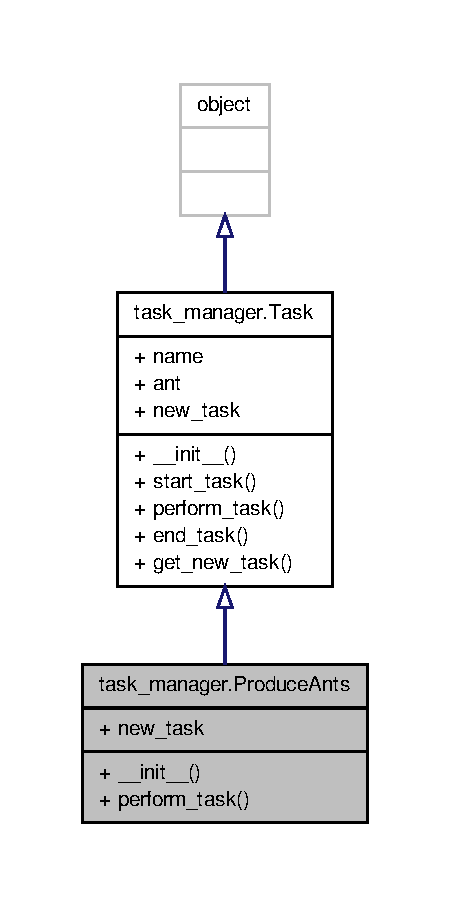
\includegraphics[width=216pt]{classtask__manager_1_1ProduceAnts__inherit__graph}
\end{center}
\end{figure}


Collaboration diagram for task\+\_\+manager.\+Produce\+Ants\+:
\nopagebreak
\begin{figure}[H]
\begin{center}
\leavevmode
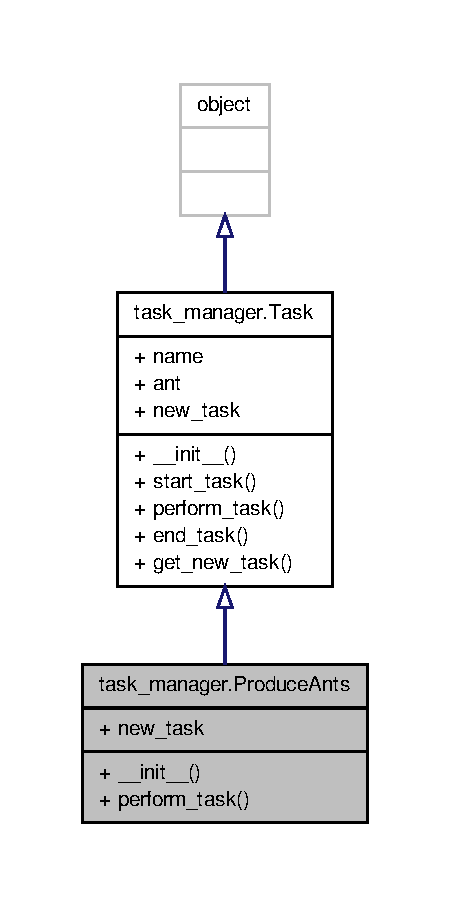
\includegraphics[width=216pt]{classtask__manager_1_1ProduceAnts__coll__graph}
\end{center}
\end{figure}
\subsection*{Public Member Functions}
\begin{DoxyCompactItemize}
\item 
def \hyperlink{classtask__manager_1_1ProduceAnts_ab154b2db66b66e0fc43d3ef5094bf73e}{\+\_\+\+\_\+init\+\_\+\+\_\+}
\item 
def \hyperlink{classtask__manager_1_1ProduceAnts_aa1636ae28589d29d45d83dd71b2dccbb}{perform\+\_\+task}
\end{DoxyCompactItemize}
\subsection*{Public Attributes}
\begin{DoxyCompactItemize}
\item 
\hyperlink{classtask__manager_1_1ProduceAnts_a52f38a28435526dc06a11cd23916ee4b}{new\+\_\+task}
\end{DoxyCompactItemize}


\subsection{Detailed Description}
\begin{DoxyVerb}Randomly produce new ants
\end{DoxyVerb}
 

Definition at line \hyperlink{task__manager_8py_source_l00322}{322} of file \hyperlink{task__manager_8py_source}{task\+\_\+manager.\+py}.



\subsection{Constructor \& Destructor Documentation}
\hypertarget{classtask__manager_1_1ProduceAnts_ab154b2db66b66e0fc43d3ef5094bf73e}{\index{task\+\_\+manager\+::\+Produce\+Ants@{task\+\_\+manager\+::\+Produce\+Ants}!\+\_\+\+\_\+init\+\_\+\+\_\+@{\+\_\+\+\_\+init\+\_\+\+\_\+}}
\index{\+\_\+\+\_\+init\+\_\+\+\_\+@{\+\_\+\+\_\+init\+\_\+\+\_\+}!task\+\_\+manager\+::\+Produce\+Ants@{task\+\_\+manager\+::\+Produce\+Ants}}
\subsubsection[{\+\_\+\+\_\+init\+\_\+\+\_\+}]{\setlength{\rightskip}{0pt plus 5cm}def task\+\_\+manager.\+Produce\+Ants.\+\_\+\+\_\+init\+\_\+\+\_\+ (
\begin{DoxyParamCaption}
\item[{}]{self, }
\item[{}]{ant}
\end{DoxyParamCaption}
)}}\label{classtask__manager_1_1ProduceAnts_ab154b2db66b66e0fc43d3ef5094bf73e}


Definition at line \hyperlink{task__manager_8py_source_l00326}{326} of file \hyperlink{task__manager_8py_source}{task\+\_\+manager.\+py}.



\subsection{Member Function Documentation}
\hypertarget{classtask__manager_1_1ProduceAnts_aa1636ae28589d29d45d83dd71b2dccbb}{\index{task\+\_\+manager\+::\+Produce\+Ants@{task\+\_\+manager\+::\+Produce\+Ants}!perform\+\_\+task@{perform\+\_\+task}}
\index{perform\+\_\+task@{perform\+\_\+task}!task\+\_\+manager\+::\+Produce\+Ants@{task\+\_\+manager\+::\+Produce\+Ants}}
\subsubsection[{perform\+\_\+task}]{\setlength{\rightskip}{0pt plus 5cm}def task\+\_\+manager.\+Produce\+Ants.\+perform\+\_\+task (
\begin{DoxyParamCaption}
\item[{}]{self}
\end{DoxyParamCaption}
)}}\label{classtask__manager_1_1ProduceAnts_aa1636ae28589d29d45d83dd71b2dccbb}
\begin{DoxyVerb}randomly produce new ants\end{DoxyVerb}
 

Definition at line \hyperlink{task__manager_8py_source_l00329}{329} of file \hyperlink{task__manager_8py_source}{task\+\_\+manager.\+py}.



\subsection{Member Data Documentation}
\hypertarget{classtask__manager_1_1ProduceAnts_a52f38a28435526dc06a11cd23916ee4b}{\index{task\+\_\+manager\+::\+Produce\+Ants@{task\+\_\+manager\+::\+Produce\+Ants}!new\+\_\+task@{new\+\_\+task}}
\index{new\+\_\+task@{new\+\_\+task}!task\+\_\+manager\+::\+Produce\+Ants@{task\+\_\+manager\+::\+Produce\+Ants}}
\subsubsection[{new\+\_\+task}]{\setlength{\rightskip}{0pt plus 5cm}task\+\_\+manager.\+Produce\+Ants.\+new\+\_\+task}}\label{classtask__manager_1_1ProduceAnts_a52f38a28435526dc06a11cd23916ee4b}


Definition at line \hyperlink{task__manager_8py_source_l00332}{332} of file \hyperlink{task__manager_8py_source}{task\+\_\+manager.\+py}.



The documentation for this class was generated from the following file\+:\begin{DoxyCompactItemize}
\item 
\hyperlink{task__manager_8py}{task\+\_\+manager.\+py}\end{DoxyCompactItemize}

\hypertarget{classants_1_1QueenAnt}{\section{ants.\+Queen\+Ant Class Reference}
\label{classants_1_1QueenAnt}\index{ants.\+Queen\+Ant@{ants.\+Queen\+Ant}}
}


Inheritance diagram for ants.\+Queen\+Ant\+:
\nopagebreak
\begin{figure}[H]
\begin{center}
\leavevmode
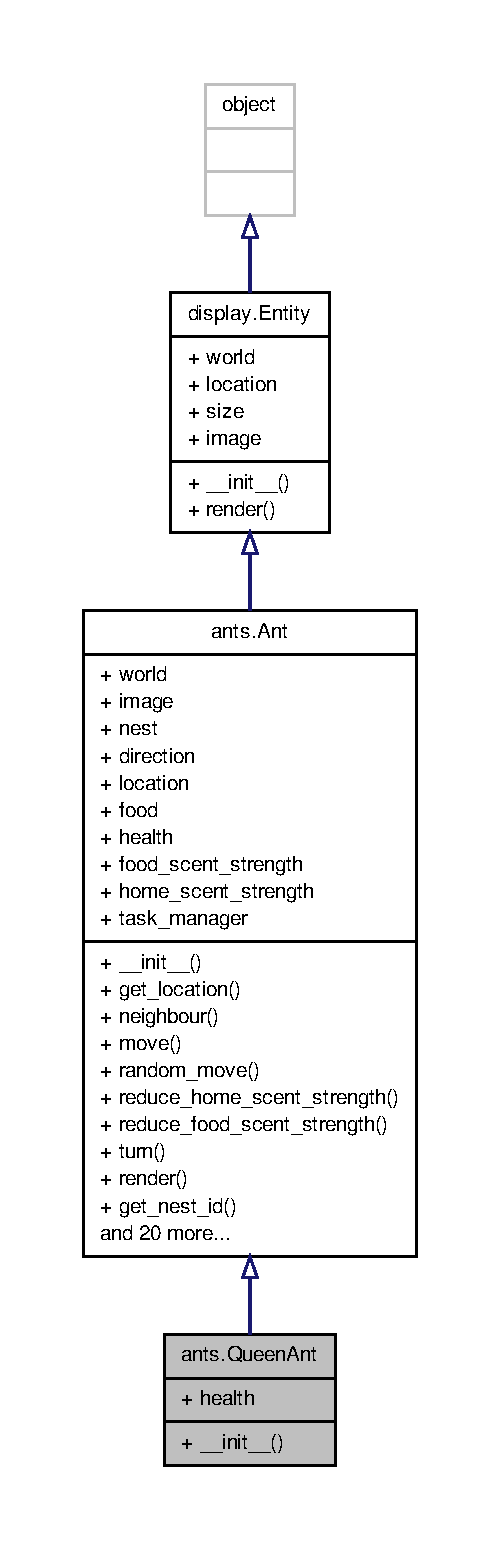
\includegraphics[height=550pt]{classants_1_1QueenAnt__inherit__graph}
\end{center}
\end{figure}


Collaboration diagram for ants.\+Queen\+Ant\+:
\nopagebreak
\begin{figure}[H]
\begin{center}
\leavevmode
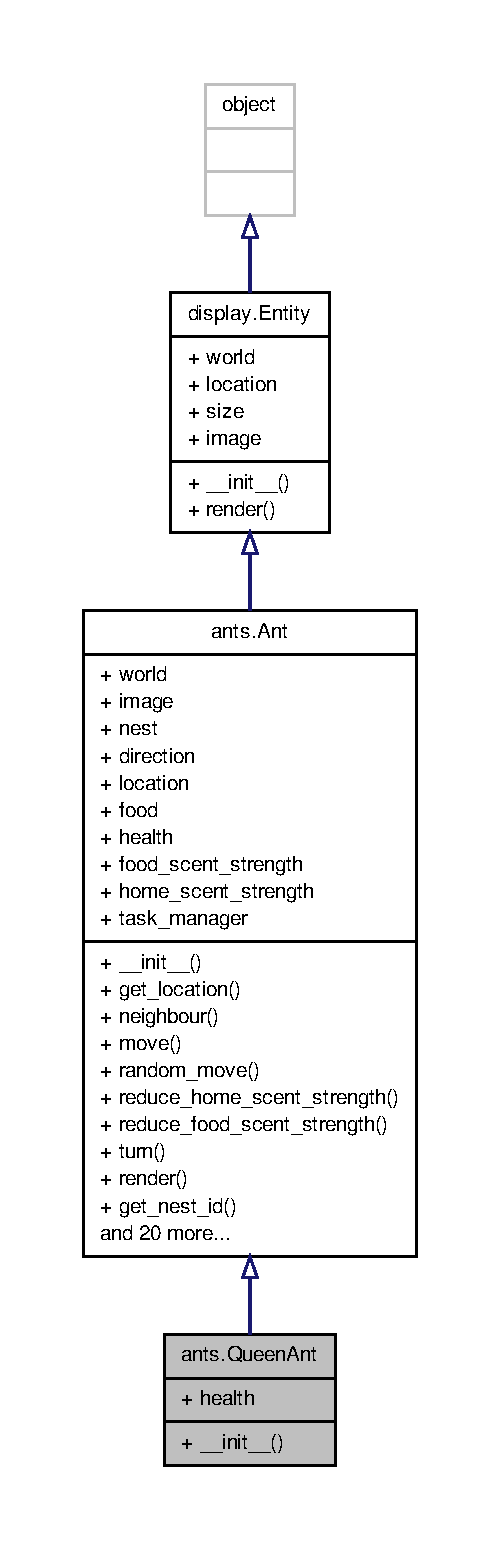
\includegraphics[height=550pt]{classants_1_1QueenAnt__coll__graph}
\end{center}
\end{figure}
\subsection*{Public Member Functions}
\begin{DoxyCompactItemize}
\item 
def \hyperlink{classants_1_1QueenAnt_aea3ff8fa90122567905806f675eb9472}{\+\_\+\+\_\+init\+\_\+\+\_\+}
\end{DoxyCompactItemize}
\subsection*{Public Attributes}
\begin{DoxyCompactItemize}
\item 
\hyperlink{classants_1_1QueenAnt_adb02e07e568bf5cf90408cb641cb5b57}{health}
\end{DoxyCompactItemize}


\subsection{Detailed Description}
\begin{DoxyVerb}Ants that produces offsprings and populates the colony
\end{DoxyVerb}
 

Definition at line \hyperlink{ants_8py_source_l00323}{323} of file \hyperlink{ants_8py_source}{ants.\+py}.



\subsection{Constructor \& Destructor Documentation}
\hypertarget{classants_1_1QueenAnt_aea3ff8fa90122567905806f675eb9472}{\index{ants\+::\+Queen\+Ant@{ants\+::\+Queen\+Ant}!\+\_\+\+\_\+init\+\_\+\+\_\+@{\+\_\+\+\_\+init\+\_\+\+\_\+}}
\index{\+\_\+\+\_\+init\+\_\+\+\_\+@{\+\_\+\+\_\+init\+\_\+\+\_\+}!ants\+::\+Queen\+Ant@{ants\+::\+Queen\+Ant}}
\subsubsection[{\+\_\+\+\_\+init\+\_\+\+\_\+}]{\setlength{\rightskip}{0pt plus 5cm}def ants.\+Queen\+Ant.\+\_\+\+\_\+init\+\_\+\+\_\+ (
\begin{DoxyParamCaption}
\item[{}]{self, }
\item[{}]{world, }
\item[{}]{image, }
\item[{}]{direction, }
\item[{}]{location, }
\item[{}]{nest}
\end{DoxyParamCaption}
)}}\label{classants_1_1QueenAnt_aea3ff8fa90122567905806f675eb9472}
\begin{DoxyVerb}Tasks assigned:
    - Find Food
    - Produce offsprings
Default task:
    - Find Food
\end{DoxyVerb}
 

Definition at line \hyperlink{ants_8py_source_l00327}{327} of file \hyperlink{ants_8py_source}{ants.\+py}.



\subsection{Member Data Documentation}
\hypertarget{classants_1_1QueenAnt_adb02e07e568bf5cf90408cb641cb5b57}{\index{ants\+::\+Queen\+Ant@{ants\+::\+Queen\+Ant}!health@{health}}
\index{health@{health}!ants\+::\+Queen\+Ant@{ants\+::\+Queen\+Ant}}
\subsubsection[{health}]{\setlength{\rightskip}{0pt plus 5cm}ants.\+Queen\+Ant.\+health}}\label{classants_1_1QueenAnt_adb02e07e568bf5cf90408cb641cb5b57}


Definition at line \hyperlink{ants_8py_source_l00339}{339} of file \hyperlink{ants_8py_source}{ants.\+py}.



The documentation for this class was generated from the following file\+:\begin{DoxyCompactItemize}
\item 
\hyperlink{ants_8py}{ants.\+py}\end{DoxyCompactItemize}

\hypertarget{classtask__manager_1_1ReturnHome}{\section{task\+\_\+manager.\+Return\+Home Class Reference}
\label{classtask__manager_1_1ReturnHome}\index{task\+\_\+manager.\+Return\+Home@{task\+\_\+manager.\+Return\+Home}}
}


Inheritance diagram for task\+\_\+manager.\+Return\+Home\+:
\nopagebreak
\begin{figure}[H]
\begin{center}
\leavevmode
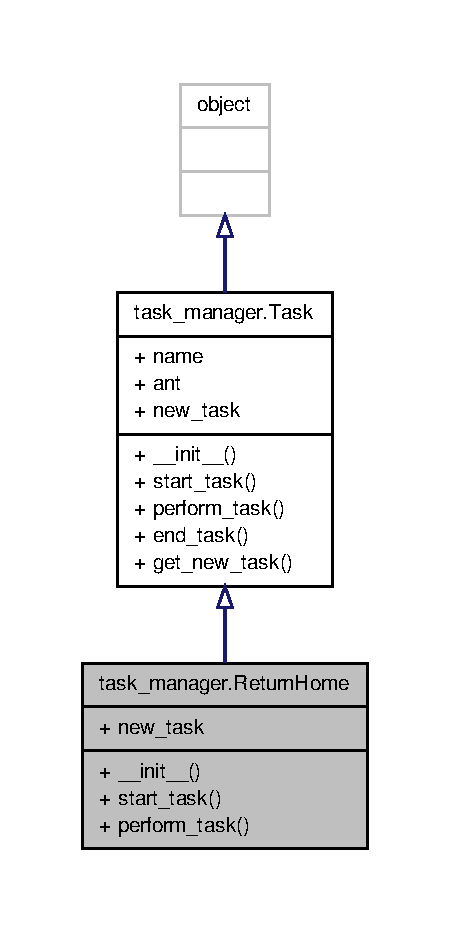
\includegraphics[width=216pt]{classtask__manager_1_1ReturnHome__inherit__graph}
\end{center}
\end{figure}


Collaboration diagram for task\+\_\+manager.\+Return\+Home\+:
\nopagebreak
\begin{figure}[H]
\begin{center}
\leavevmode
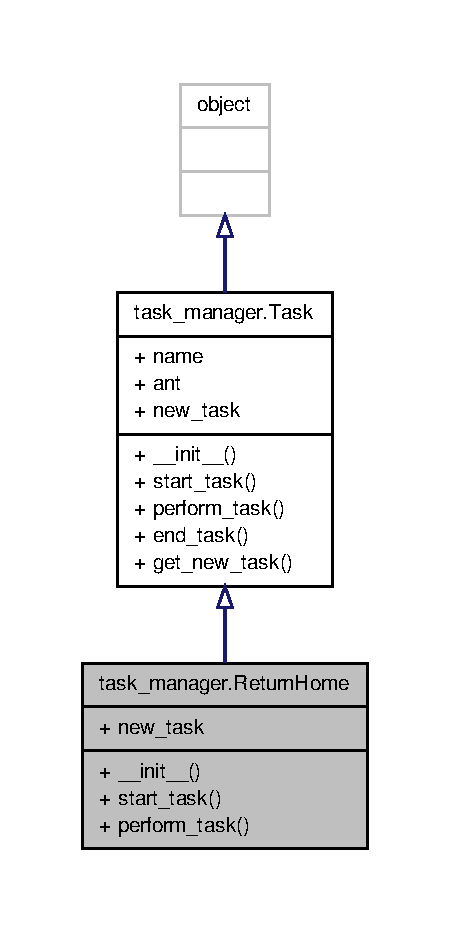
\includegraphics[width=216pt]{classtask__manager_1_1ReturnHome__coll__graph}
\end{center}
\end{figure}
\subsection*{Public Member Functions}
\begin{DoxyCompactItemize}
\item 
def \hyperlink{classtask__manager_1_1ReturnHome_ada66b785625008db20221e1b53d419f6}{\+\_\+\+\_\+init\+\_\+\+\_\+}
\item 
def \hyperlink{classtask__manager_1_1ReturnHome_a8201892f7668c2ca1e7c08f2a51c4309}{start\+\_\+task}
\item 
def \hyperlink{classtask__manager_1_1ReturnHome_ab9d2b69cbefdeaf308df564c13f5aac2}{perform\+\_\+task}
\end{DoxyCompactItemize}
\subsection*{Public Attributes}
\begin{DoxyCompactItemize}
\item 
\hyperlink{classtask__manager_1_1ReturnHome_afd37383d07987cb20f716cfe86b7b957}{new\+\_\+task}
\end{DoxyCompactItemize}


\subsection{Detailed Description}
\begin{DoxyVerb}Return home if the ant is roaming outside
\end{DoxyVerb}
 

Definition at line \hyperlink{task__manager_8py_source_l00261}{261} of file \hyperlink{task__manager_8py_source}{task\+\_\+manager.\+py}.



\subsection{Constructor \& Destructor Documentation}
\hypertarget{classtask__manager_1_1ReturnHome_ada66b785625008db20221e1b53d419f6}{\index{task\+\_\+manager\+::\+Return\+Home@{task\+\_\+manager\+::\+Return\+Home}!\+\_\+\+\_\+init\+\_\+\+\_\+@{\+\_\+\+\_\+init\+\_\+\+\_\+}}
\index{\+\_\+\+\_\+init\+\_\+\+\_\+@{\+\_\+\+\_\+init\+\_\+\+\_\+}!task\+\_\+manager\+::\+Return\+Home@{task\+\_\+manager\+::\+Return\+Home}}
\subsubsection[{\+\_\+\+\_\+init\+\_\+\+\_\+}]{\setlength{\rightskip}{0pt plus 5cm}def task\+\_\+manager.\+Return\+Home.\+\_\+\+\_\+init\+\_\+\+\_\+ (
\begin{DoxyParamCaption}
\item[{}]{self, }
\item[{}]{ant}
\end{DoxyParamCaption}
)}}\label{classtask__manager_1_1ReturnHome_ada66b785625008db20221e1b53d419f6}


Definition at line \hyperlink{task__manager_8py_source_l00265}{265} of file \hyperlink{task__manager_8py_source}{task\+\_\+manager.\+py}.



\subsection{Member Function Documentation}
\hypertarget{classtask__manager_1_1ReturnHome_ab9d2b69cbefdeaf308df564c13f5aac2}{\index{task\+\_\+manager\+::\+Return\+Home@{task\+\_\+manager\+::\+Return\+Home}!perform\+\_\+task@{perform\+\_\+task}}
\index{perform\+\_\+task@{perform\+\_\+task}!task\+\_\+manager\+::\+Return\+Home@{task\+\_\+manager\+::\+Return\+Home}}
\subsubsection[{perform\+\_\+task}]{\setlength{\rightskip}{0pt plus 5cm}def task\+\_\+manager.\+Return\+Home.\+perform\+\_\+task (
\begin{DoxyParamCaption}
\item[{}]{self}
\end{DoxyParamCaption}
)}}\label{classtask__manager_1_1ReturnHome_ab9d2b69cbefdeaf308df564c13f5aac2}
\begin{DoxyVerb}Follow home trail and return home
\end{DoxyVerb}
 

Definition at line \hyperlink{task__manager_8py_source_l00272}{272} of file \hyperlink{task__manager_8py_source}{task\+\_\+manager.\+py}.

\hypertarget{classtask__manager_1_1ReturnHome_a8201892f7668c2ca1e7c08f2a51c4309}{\index{task\+\_\+manager\+::\+Return\+Home@{task\+\_\+manager\+::\+Return\+Home}!start\+\_\+task@{start\+\_\+task}}
\index{start\+\_\+task@{start\+\_\+task}!task\+\_\+manager\+::\+Return\+Home@{task\+\_\+manager\+::\+Return\+Home}}
\subsubsection[{start\+\_\+task}]{\setlength{\rightskip}{0pt plus 5cm}def task\+\_\+manager.\+Return\+Home.\+start\+\_\+task (
\begin{DoxyParamCaption}
\item[{}]{self}
\end{DoxyParamCaption}
)}}\label{classtask__manager_1_1ReturnHome_a8201892f7668c2ca1e7c08f2a51c4309}


Definition at line \hyperlink{task__manager_8py_source_l00268}{268} of file \hyperlink{task__manager_8py_source}{task\+\_\+manager.\+py}.



\subsection{Member Data Documentation}
\hypertarget{classtask__manager_1_1ReturnHome_afd37383d07987cb20f716cfe86b7b957}{\index{task\+\_\+manager\+::\+Return\+Home@{task\+\_\+manager\+::\+Return\+Home}!new\+\_\+task@{new\+\_\+task}}
\index{new\+\_\+task@{new\+\_\+task}!task\+\_\+manager\+::\+Return\+Home@{task\+\_\+manager\+::\+Return\+Home}}
\subsubsection[{new\+\_\+task}]{\setlength{\rightskip}{0pt plus 5cm}task\+\_\+manager.\+Return\+Home.\+new\+\_\+task}}\label{classtask__manager_1_1ReturnHome_afd37383d07987cb20f716cfe86b7b957}


Definition at line \hyperlink{task__manager_8py_source_l00283}{283} of file \hyperlink{task__manager_8py_source}{task\+\_\+manager.\+py}.



The documentation for this class was generated from the following file\+:\begin{DoxyCompactItemize}
\item 
\hyperlink{task__manager_8py}{task\+\_\+manager.\+py}\end{DoxyCompactItemize}

\hypertarget{classcontroller_1_1Simulation}{\section{controller.\+Simulation Class Reference}
\label{classcontroller_1_1Simulation}\index{controller.\+Simulation@{controller.\+Simulation}}
}


Collaboration diagram for controller.\+Simulation\+:\nopagebreak
\begin{figure}[H]
\begin{center}
\leavevmode
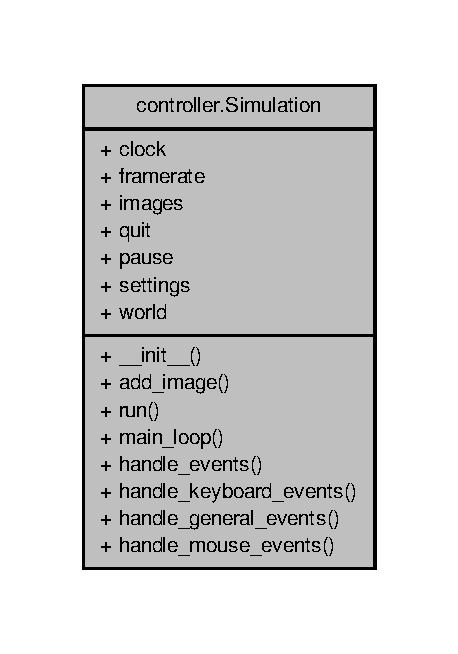
\includegraphics[width=184pt]{classcontroller_1_1Simulation__coll__graph}
\end{center}
\end{figure}
\subsection*{Public Member Functions}
\begin{DoxyCompactItemize}
\item 
def \hyperlink{classcontroller_1_1Simulation_a0d3a98e6f630a62f18aa5c0c35846381}{\+\_\+\+\_\+init\+\_\+\+\_\+}
\item 
def \hyperlink{classcontroller_1_1Simulation_a91674f018c921725aa36ec25396a7304}{add\+\_\+image}
\item 
def \hyperlink{classcontroller_1_1Simulation_a4cbf2928d3f930f4b8cad9c0e64c2524}{run}
\item 
def \hyperlink{classcontroller_1_1Simulation_ad86d932f45e2b80ec5336da7c6e6e085}{main\+\_\+loop}
\item 
def \hyperlink{classcontroller_1_1Simulation_ad3eb13a30931a88958e3c0c7b5b545a5}{handle\+\_\+events}
\end{DoxyCompactItemize}
\subsection*{Public Attributes}
\begin{DoxyCompactItemize}
\item 
\hyperlink{classcontroller_1_1Simulation_a21dd9474d46d4afa868c0bd60cea128b}{clock}
\item 
\hyperlink{classcontroller_1_1Simulation_a2bc2a4bb3e974bc7b73be75b49701d9f}{framerate}
\item 
\hyperlink{classcontroller_1_1Simulation_af13461f42bfe6ca017f59e13e57c354e}{images}
\item 
\hyperlink{classcontroller_1_1Simulation_a35d0ffc695295c3b509bd5bc2bdbac9b}{quit}
\item 
\hyperlink{classcontroller_1_1Simulation_a5d368ffc3eee12c8c36839ee5bce3644}{settings}
\item 
\hyperlink{classcontroller_1_1Simulation_a2ba0c3cf1949a98dd920f6097953c1f5}{world}
\end{DoxyCompactItemize}


\subsection{Detailed Description}
\begin{DoxyVerb}Controls the simulation

    - Runs the main loop
    - Detects mouse, keyboard and other events
    - Loads the necessary images
    - Controls the framerate of the smiulation
\end{DoxyVerb}
 

Definition at line \hyperlink{controller_8py_source_l00005}{5} of file \hyperlink{controller_8py_source}{controller.\+py}.



\subsection{Constructor \& Destructor Documentation}
\hypertarget{classcontroller_1_1Simulation_a0d3a98e6f630a62f18aa5c0c35846381}{\index{controller\+::\+Simulation@{controller\+::\+Simulation}!\+\_\+\+\_\+init\+\_\+\+\_\+@{\+\_\+\+\_\+init\+\_\+\+\_\+}}
\index{\+\_\+\+\_\+init\+\_\+\+\_\+@{\+\_\+\+\_\+init\+\_\+\+\_\+}!controller\+::\+Simulation@{controller\+::\+Simulation}}
\subsubsection[{\+\_\+\+\_\+init\+\_\+\+\_\+}]{\setlength{\rightskip}{0pt plus 5cm}def controller.\+Simulation.\+\_\+\+\_\+init\+\_\+\+\_\+ (
\begin{DoxyParamCaption}
\item[{}]{self}
\end{DoxyParamCaption}
)}}\label{classcontroller_1_1Simulation_a0d3a98e6f630a62f18aa5c0c35846381}


Definition at line \hyperlink{controller_8py_source_l00013}{13} of file \hyperlink{controller_8py_source}{controller.\+py}.



\subsection{Member Function Documentation}
\hypertarget{classcontroller_1_1Simulation_a91674f018c921725aa36ec25396a7304}{\index{controller\+::\+Simulation@{controller\+::\+Simulation}!add\+\_\+image@{add\+\_\+image}}
\index{add\+\_\+image@{add\+\_\+image}!controller\+::\+Simulation@{controller\+::\+Simulation}}
\subsubsection[{add\+\_\+image}]{\setlength{\rightskip}{0pt plus 5cm}def controller.\+Simulation.\+add\+\_\+image (
\begin{DoxyParamCaption}
\item[{}]{self, }
\item[{}]{name, }
\item[{}]{path}
\end{DoxyParamCaption}
)}}\label{classcontroller_1_1Simulation_a91674f018c921725aa36ec25396a7304}
\begin{DoxyVerb}Loads an image\end{DoxyVerb}
 

Definition at line \hyperlink{controller_8py_source_l00037}{37} of file \hyperlink{controller_8py_source}{controller.\+py}.

\hypertarget{classcontroller_1_1Simulation_ad3eb13a30931a88958e3c0c7b5b545a5}{\index{controller\+::\+Simulation@{controller\+::\+Simulation}!handle\+\_\+events@{handle\+\_\+events}}
\index{handle\+\_\+events@{handle\+\_\+events}!controller\+::\+Simulation@{controller\+::\+Simulation}}
\subsubsection[{handle\+\_\+events}]{\setlength{\rightskip}{0pt plus 5cm}def controller.\+Simulation.\+handle\+\_\+events (
\begin{DoxyParamCaption}
\item[{}]{self}
\end{DoxyParamCaption}
)}}\label{classcontroller_1_1Simulation_ad3eb13a30931a88958e3c0c7b5b545a5}
\begin{DoxyVerb}Handles all keyboard, mouse and events like QUIT, etc\end{DoxyVerb}
 

Definition at line \hyperlink{controller_8py_source_l00059}{59} of file \hyperlink{controller_8py_source}{controller.\+py}.

\hypertarget{classcontroller_1_1Simulation_ad86d932f45e2b80ec5336da7c6e6e085}{\index{controller\+::\+Simulation@{controller\+::\+Simulation}!main\+\_\+loop@{main\+\_\+loop}}
\index{main\+\_\+loop@{main\+\_\+loop}!controller\+::\+Simulation@{controller\+::\+Simulation}}
\subsubsection[{main\+\_\+loop}]{\setlength{\rightskip}{0pt plus 5cm}def controller.\+Simulation.\+main\+\_\+loop (
\begin{DoxyParamCaption}
\item[{}]{self}
\end{DoxyParamCaption}
)}}\label{classcontroller_1_1Simulation_ad86d932f45e2b80ec5336da7c6e6e085}
\begin{DoxyVerb}Updates the simulation
    - Draws the world and update it
    - Handles all user events
    - Controls frame rate
\end{DoxyVerb}
 

Definition at line \hyperlink{controller_8py_source_l00046}{46} of file \hyperlink{controller_8py_source}{controller.\+py}.

\hypertarget{classcontroller_1_1Simulation_a4cbf2928d3f930f4b8cad9c0e64c2524}{\index{controller\+::\+Simulation@{controller\+::\+Simulation}!run@{run}}
\index{run@{run}!controller\+::\+Simulation@{controller\+::\+Simulation}}
\subsubsection[{run}]{\setlength{\rightskip}{0pt plus 5cm}def controller.\+Simulation.\+run (
\begin{DoxyParamCaption}
\item[{}]{self}
\end{DoxyParamCaption}
)}}\label{classcontroller_1_1Simulation_a4cbf2928d3f930f4b8cad9c0e64c2524}
\begin{DoxyVerb}Runs the main loop till the user quits\end{DoxyVerb}
 

Definition at line \hyperlink{controller_8py_source_l00041}{41} of file \hyperlink{controller_8py_source}{controller.\+py}.



\subsection{Member Data Documentation}
\hypertarget{classcontroller_1_1Simulation_a21dd9474d46d4afa868c0bd60cea128b}{\index{controller\+::\+Simulation@{controller\+::\+Simulation}!clock@{clock}}
\index{clock@{clock}!controller\+::\+Simulation@{controller\+::\+Simulation}}
\subsubsection[{clock}]{\setlength{\rightskip}{0pt plus 5cm}controller.\+Simulation.\+clock}}\label{classcontroller_1_1Simulation_a21dd9474d46d4afa868c0bd60cea128b}


Definition at line \hyperlink{controller_8py_source_l00014}{14} of file \hyperlink{controller_8py_source}{controller.\+py}.

\hypertarget{classcontroller_1_1Simulation_a2bc2a4bb3e974bc7b73be75b49701d9f}{\index{controller\+::\+Simulation@{controller\+::\+Simulation}!framerate@{framerate}}
\index{framerate@{framerate}!controller\+::\+Simulation@{controller\+::\+Simulation}}
\subsubsection[{framerate}]{\setlength{\rightskip}{0pt plus 5cm}controller.\+Simulation.\+framerate}}\label{classcontroller_1_1Simulation_a2bc2a4bb3e974bc7b73be75b49701d9f}


Definition at line \hyperlink{controller_8py_source_l00015}{15} of file \hyperlink{controller_8py_source}{controller.\+py}.

\hypertarget{classcontroller_1_1Simulation_af13461f42bfe6ca017f59e13e57c354e}{\index{controller\+::\+Simulation@{controller\+::\+Simulation}!images@{images}}
\index{images@{images}!controller\+::\+Simulation@{controller\+::\+Simulation}}
\subsubsection[{images}]{\setlength{\rightskip}{0pt plus 5cm}controller.\+Simulation.\+images}}\label{classcontroller_1_1Simulation_af13461f42bfe6ca017f59e13e57c354e}


Definition at line \hyperlink{controller_8py_source_l00016}{16} of file \hyperlink{controller_8py_source}{controller.\+py}.

\hypertarget{classcontroller_1_1Simulation_a35d0ffc695295c3b509bd5bc2bdbac9b}{\index{controller\+::\+Simulation@{controller\+::\+Simulation}!quit@{quit}}
\index{quit@{quit}!controller\+::\+Simulation@{controller\+::\+Simulation}}
\subsubsection[{quit}]{\setlength{\rightskip}{0pt plus 5cm}controller.\+Simulation.\+quit}}\label{classcontroller_1_1Simulation_a35d0ffc695295c3b509bd5bc2bdbac9b}


Definition at line \hyperlink{controller_8py_source_l00018}{18} of file \hyperlink{controller_8py_source}{controller.\+py}.

\hypertarget{classcontroller_1_1Simulation_a5d368ffc3eee12c8c36839ee5bce3644}{\index{controller\+::\+Simulation@{controller\+::\+Simulation}!settings@{settings}}
\index{settings@{settings}!controller\+::\+Simulation@{controller\+::\+Simulation}}
\subsubsection[{settings}]{\setlength{\rightskip}{0pt plus 5cm}controller.\+Simulation.\+settings}}\label{classcontroller_1_1Simulation_a5d368ffc3eee12c8c36839ee5bce3644}


Definition at line \hyperlink{controller_8py_source_l00029}{29} of file \hyperlink{controller_8py_source}{controller.\+py}.

\hypertarget{classcontroller_1_1Simulation_a2ba0c3cf1949a98dd920f6097953c1f5}{\index{controller\+::\+Simulation@{controller\+::\+Simulation}!world@{world}}
\index{world@{world}!controller\+::\+Simulation@{controller\+::\+Simulation}}
\subsubsection[{world}]{\setlength{\rightskip}{0pt plus 5cm}controller.\+Simulation.\+world}}\label{classcontroller_1_1Simulation_a2ba0c3cf1949a98dd920f6097953c1f5}


Definition at line \hyperlink{controller_8py_source_l00035}{35} of file \hyperlink{controller_8py_source}{controller.\+py}.



The documentation for this class was generated from the following file\+:\begin{DoxyCompactItemize}
\item 
\hyperlink{controller_8py}{controller.\+py}\end{DoxyCompactItemize}

\hypertarget{classants_1_1SoldierAnt}{\section{ants.\+Soldier\+Ant Class Reference}
\label{classants_1_1SoldierAnt}\index{ants.\+Soldier\+Ant@{ants.\+Soldier\+Ant}}
}


Inheritance diagram for ants.\+Soldier\+Ant\+:
\nopagebreak
\begin{figure}[H]
\begin{center}
\leavevmode
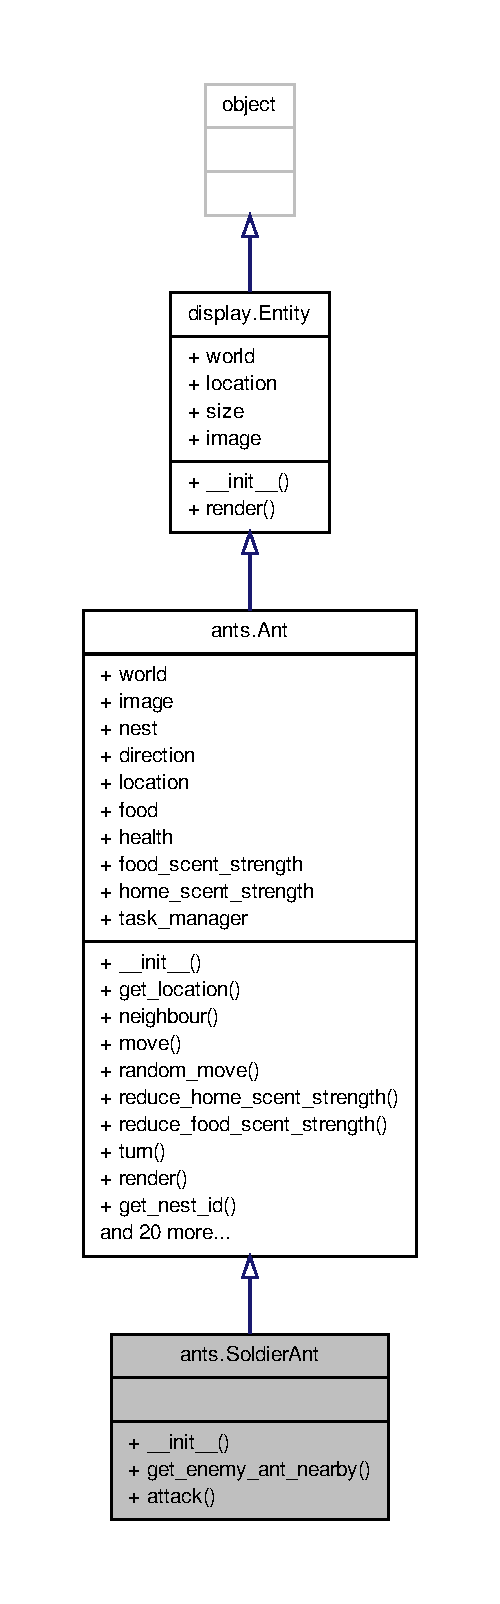
\includegraphics[height=550pt]{classants_1_1SoldierAnt__inherit__graph}
\end{center}
\end{figure}


Collaboration diagram for ants.\+Soldier\+Ant\+:
\nopagebreak
\begin{figure}[H]
\begin{center}
\leavevmode
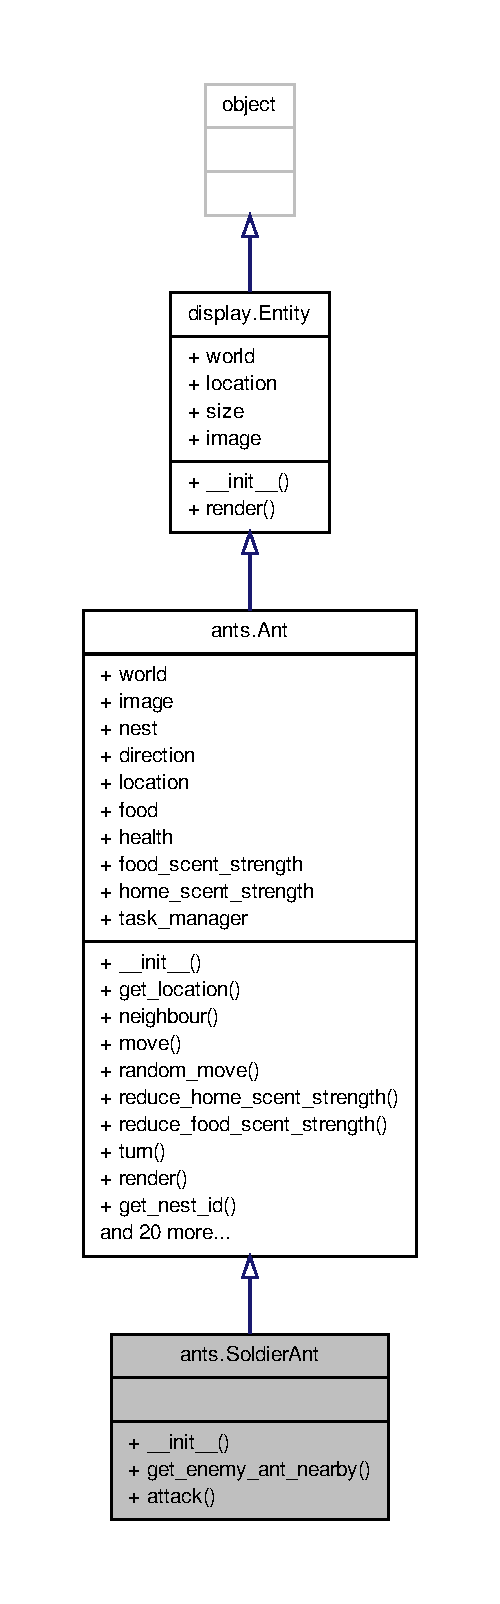
\includegraphics[height=550pt]{classants_1_1SoldierAnt__coll__graph}
\end{center}
\end{figure}
\subsection*{Public Member Functions}
\begin{DoxyCompactItemize}
\item 
def \hyperlink{classants_1_1SoldierAnt_adaaa2dc645cd3f4c190a86caa7e18f35}{\+\_\+\+\_\+init\+\_\+\+\_\+}
\item 
def \hyperlink{classants_1_1SoldierAnt_aa3d00e2aca5711f0b5784fd2ec0f4989}{get\+\_\+enemy\+\_\+ant\+\_\+nearby}
\item 
def \hyperlink{classants_1_1SoldierAnt_a66062d822fc415e73332f7b13cf853c8}{attack}
\end{DoxyCompactItemize}
\subsection*{Additional Inherited Members}


\subsection{Detailed Description}
\begin{DoxyVerb}Ants that produces offsprings and populates the colony\end{DoxyVerb}
 

Definition at line \hyperlink{ants_8py_source_l00342}{342} of file \hyperlink{ants_8py_source}{ants.\+py}.



\subsection{Constructor \& Destructor Documentation}
\hypertarget{classants_1_1SoldierAnt_adaaa2dc645cd3f4c190a86caa7e18f35}{\index{ants\+::\+Soldier\+Ant@{ants\+::\+Soldier\+Ant}!\+\_\+\+\_\+init\+\_\+\+\_\+@{\+\_\+\+\_\+init\+\_\+\+\_\+}}
\index{\+\_\+\+\_\+init\+\_\+\+\_\+@{\+\_\+\+\_\+init\+\_\+\+\_\+}!ants\+::\+Soldier\+Ant@{ants\+::\+Soldier\+Ant}}
\subsubsection[{\+\_\+\+\_\+init\+\_\+\+\_\+}]{\setlength{\rightskip}{0pt plus 5cm}def ants.\+Soldier\+Ant.\+\_\+\+\_\+init\+\_\+\+\_\+ (
\begin{DoxyParamCaption}
\item[{}]{self, }
\item[{}]{world, }
\item[{}]{image, }
\item[{}]{direction, }
\item[{}]{location, }
\item[{}]{nest}
\end{DoxyParamCaption}
)}}\label{classants_1_1SoldierAnt_adaaa2dc645cd3f4c190a86caa7e18f35}
\begin{DoxyVerb}Tasks assigned:
    - Guard nest
    - Return home
Default task:
    - Guard nest
\end{DoxyVerb}
 

Definition at line \hyperlink{ants_8py_source_l00344}{344} of file \hyperlink{ants_8py_source}{ants.\+py}.



\subsection{Member Function Documentation}
\hypertarget{classants_1_1SoldierAnt_a66062d822fc415e73332f7b13cf853c8}{\index{ants\+::\+Soldier\+Ant@{ants\+::\+Soldier\+Ant}!attack@{attack}}
\index{attack@{attack}!ants\+::\+Soldier\+Ant@{ants\+::\+Soldier\+Ant}}
\subsubsection[{attack}]{\setlength{\rightskip}{0pt plus 5cm}def ants.\+Soldier\+Ant.\+attack (
\begin{DoxyParamCaption}
\item[{}]{self, }
\item[{}]{ant}
\end{DoxyParamCaption}
)}}\label{classants_1_1SoldierAnt_a66062d822fc415e73332f7b13cf853c8}


Definition at line \hyperlink{ants_8py_source_l00366}{366} of file \hyperlink{ants_8py_source}{ants.\+py}.

\hypertarget{classants_1_1SoldierAnt_aa3d00e2aca5711f0b5784fd2ec0f4989}{\index{ants\+::\+Soldier\+Ant@{ants\+::\+Soldier\+Ant}!get\+\_\+enemy\+\_\+ant\+\_\+nearby@{get\+\_\+enemy\+\_\+ant\+\_\+nearby}}
\index{get\+\_\+enemy\+\_\+ant\+\_\+nearby@{get\+\_\+enemy\+\_\+ant\+\_\+nearby}!ants\+::\+Soldier\+Ant@{ants\+::\+Soldier\+Ant}}
\subsubsection[{get\+\_\+enemy\+\_\+ant\+\_\+nearby}]{\setlength{\rightskip}{0pt plus 5cm}def ants.\+Soldier\+Ant.\+get\+\_\+enemy\+\_\+ant\+\_\+nearby (
\begin{DoxyParamCaption}
\item[{}]{self}
\end{DoxyParamCaption}
)}}\label{classants_1_1SoldierAnt_aa3d00e2aca5711f0b5784fd2ec0f4989}
\begin{DoxyVerb}Returns one enemy ant nearby at random
\end{DoxyVerb}
 

Definition at line \hyperlink{ants_8py_source_l00357}{357} of file \hyperlink{ants_8py_source}{ants.\+py}.



The documentation for this class was generated from the following file\+:\begin{DoxyCompactItemize}
\item 
\hyperlink{ants_8py}{ants.\+py}\end{DoxyCompactItemize}

\hypertarget{classtask__manager_1_1TakeFood}{\section{task\+\_\+manager.\+Take\+Food Class Reference}
\label{classtask__manager_1_1TakeFood}\index{task\+\_\+manager.\+Take\+Food@{task\+\_\+manager.\+Take\+Food}}
}


Inheritance diagram for task\+\_\+manager.\+Take\+Food\+:\nopagebreak
\begin{figure}[H]
\begin{center}
\leavevmode
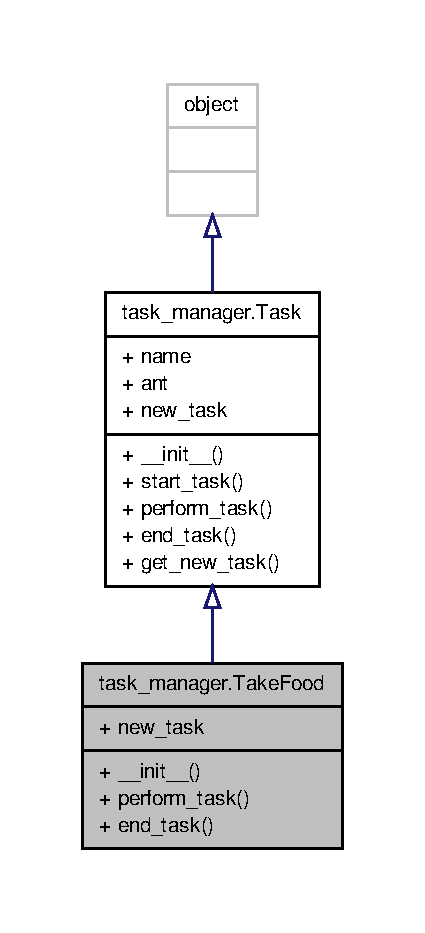
\includegraphics[width=204pt]{classtask__manager_1_1TakeFood__inherit__graph}
\end{center}
\end{figure}


Collaboration diagram for task\+\_\+manager.\+Take\+Food\+:\nopagebreak
\begin{figure}[H]
\begin{center}
\leavevmode
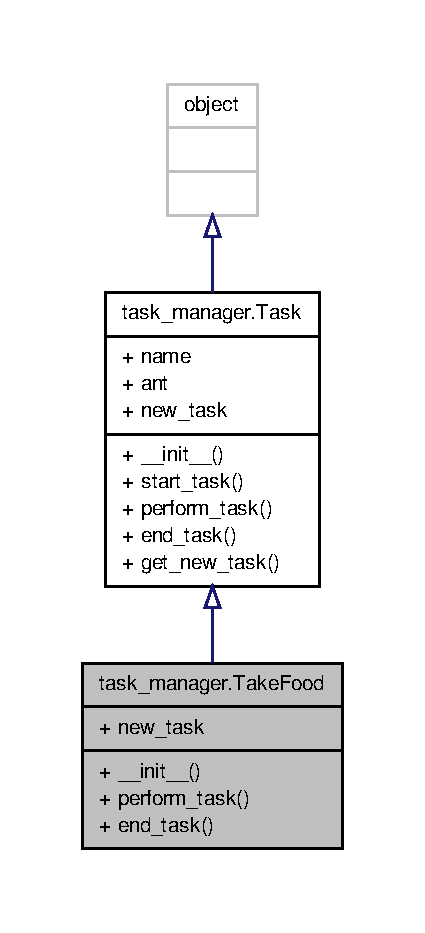
\includegraphics[width=204pt]{classtask__manager_1_1TakeFood__coll__graph}
\end{center}
\end{figure}
\subsection*{Public Member Functions}
\begin{DoxyCompactItemize}
\item 
def \hyperlink{classtask__manager_1_1TakeFood_a4c5cc2bb37fc196bc5cb34f56fa62a29}{\+\_\+\+\_\+init\+\_\+\+\_\+}
\item 
def \hyperlink{classtask__manager_1_1TakeFood_af42eebb5d9ee945cafd05908d478bab3}{perform\+\_\+task}
\item 
def \hyperlink{classtask__manager_1_1TakeFood_a01c78eece0496ccd7c7badde7ce848b4}{end\+\_\+task}
\end{DoxyCompactItemize}
\subsection*{Public Attributes}
\begin{DoxyCompactItemize}
\item 
\hyperlink{classtask__manager_1_1TakeFood_a592252f7a2b882cf283c9da9cbab07a2}{new\+\_\+task}
\end{DoxyCompactItemize}


\subsection{Detailed Description}
\begin{DoxyVerb}Gathering Food Task\end{DoxyVerb}
 

Definition at line \hyperlink{task__manager_8py_source_l00103}{103} of file \hyperlink{task__manager_8py_source}{task\+\_\+manager.\+py}.



\subsection{Constructor \& Destructor Documentation}
\hypertarget{classtask__manager_1_1TakeFood_a4c5cc2bb37fc196bc5cb34f56fa62a29}{\index{task\+\_\+manager\+::\+Take\+Food@{task\+\_\+manager\+::\+Take\+Food}!\+\_\+\+\_\+init\+\_\+\+\_\+@{\+\_\+\+\_\+init\+\_\+\+\_\+}}
\index{\+\_\+\+\_\+init\+\_\+\+\_\+@{\+\_\+\+\_\+init\+\_\+\+\_\+}!task\+\_\+manager\+::\+Take\+Food@{task\+\_\+manager\+::\+Take\+Food}}
\subsubsection[{\+\_\+\+\_\+init\+\_\+\+\_\+}]{\setlength{\rightskip}{0pt plus 5cm}def task\+\_\+manager.\+Take\+Food.\+\_\+\+\_\+init\+\_\+\+\_\+ (
\begin{DoxyParamCaption}
\item[{}]{self, }
\item[{}]{ant}
\end{DoxyParamCaption}
)}}\label{classtask__manager_1_1TakeFood_a4c5cc2bb37fc196bc5cb34f56fa62a29}


Definition at line \hyperlink{task__manager_8py_source_l00105}{105} of file \hyperlink{task__manager_8py_source}{task\+\_\+manager.\+py}.



\subsection{Member Function Documentation}
\hypertarget{classtask__manager_1_1TakeFood_a01c78eece0496ccd7c7badde7ce848b4}{\index{task\+\_\+manager\+::\+Take\+Food@{task\+\_\+manager\+::\+Take\+Food}!end\+\_\+task@{end\+\_\+task}}
\index{end\+\_\+task@{end\+\_\+task}!task\+\_\+manager\+::\+Take\+Food@{task\+\_\+manager\+::\+Take\+Food}}
\subsubsection[{end\+\_\+task}]{\setlength{\rightskip}{0pt plus 5cm}def task\+\_\+manager.\+Take\+Food.\+end\+\_\+task (
\begin{DoxyParamCaption}
\item[{}]{self}
\end{DoxyParamCaption}
)}}\label{classtask__manager_1_1TakeFood_a01c78eece0496ccd7c7badde7ce848b4}
\begin{DoxyVerb}Increase food_scent_strength
and reduce home_scent_strength\end{DoxyVerb}
 

Definition at line \hyperlink{task__manager_8py_source_l00119}{119} of file \hyperlink{task__manager_8py_source}{task\+\_\+manager.\+py}.

\hypertarget{classtask__manager_1_1TakeFood_af42eebb5d9ee945cafd05908d478bab3}{\index{task\+\_\+manager\+::\+Take\+Food@{task\+\_\+manager\+::\+Take\+Food}!perform\+\_\+task@{perform\+\_\+task}}
\index{perform\+\_\+task@{perform\+\_\+task}!task\+\_\+manager\+::\+Take\+Food@{task\+\_\+manager\+::\+Take\+Food}}
\subsubsection[{perform\+\_\+task}]{\setlength{\rightskip}{0pt plus 5cm}def task\+\_\+manager.\+Take\+Food.\+perform\+\_\+task (
\begin{DoxyParamCaption}
\item[{}]{self}
\end{DoxyParamCaption}
)}}\label{classtask__manager_1_1TakeFood_af42eebb5d9ee945cafd05908d478bab3}
\begin{DoxyVerb}Take food if available otherwise return to explore mode\end{DoxyVerb}
 

Definition at line \hyperlink{task__manager_8py_source_l00108}{108} of file \hyperlink{task__manager_8py_source}{task\+\_\+manager.\+py}.



\subsection{Member Data Documentation}
\hypertarget{classtask__manager_1_1TakeFood_a592252f7a2b882cf283c9da9cbab07a2}{\index{task\+\_\+manager\+::\+Take\+Food@{task\+\_\+manager\+::\+Take\+Food}!new\+\_\+task@{new\+\_\+task}}
\index{new\+\_\+task@{new\+\_\+task}!task\+\_\+manager\+::\+Take\+Food@{task\+\_\+manager\+::\+Take\+Food}}
\subsubsection[{new\+\_\+task}]{\setlength{\rightskip}{0pt plus 5cm}task\+\_\+manager.\+Take\+Food.\+new\+\_\+task}}\label{classtask__manager_1_1TakeFood_a592252f7a2b882cf283c9da9cbab07a2}


Definition at line \hyperlink{task__manager_8py_source_l00115}{115} of file \hyperlink{task__manager_8py_source}{task\+\_\+manager.\+py}.



The documentation for this class was generated from the following file\+:\begin{DoxyCompactItemize}
\item 
\hyperlink{task__manager_8py}{task\+\_\+manager.\+py}\end{DoxyCompactItemize}

\hypertarget{classtask__manager_1_1Task}{\section{task\+\_\+manager.\+Task Class Reference}
\label{classtask__manager_1_1Task}\index{task\+\_\+manager.\+Task@{task\+\_\+manager.\+Task}}
}


Inheritance diagram for task\+\_\+manager.\+Task\+:
\nopagebreak
\begin{figure}[H]
\begin{center}
\leavevmode
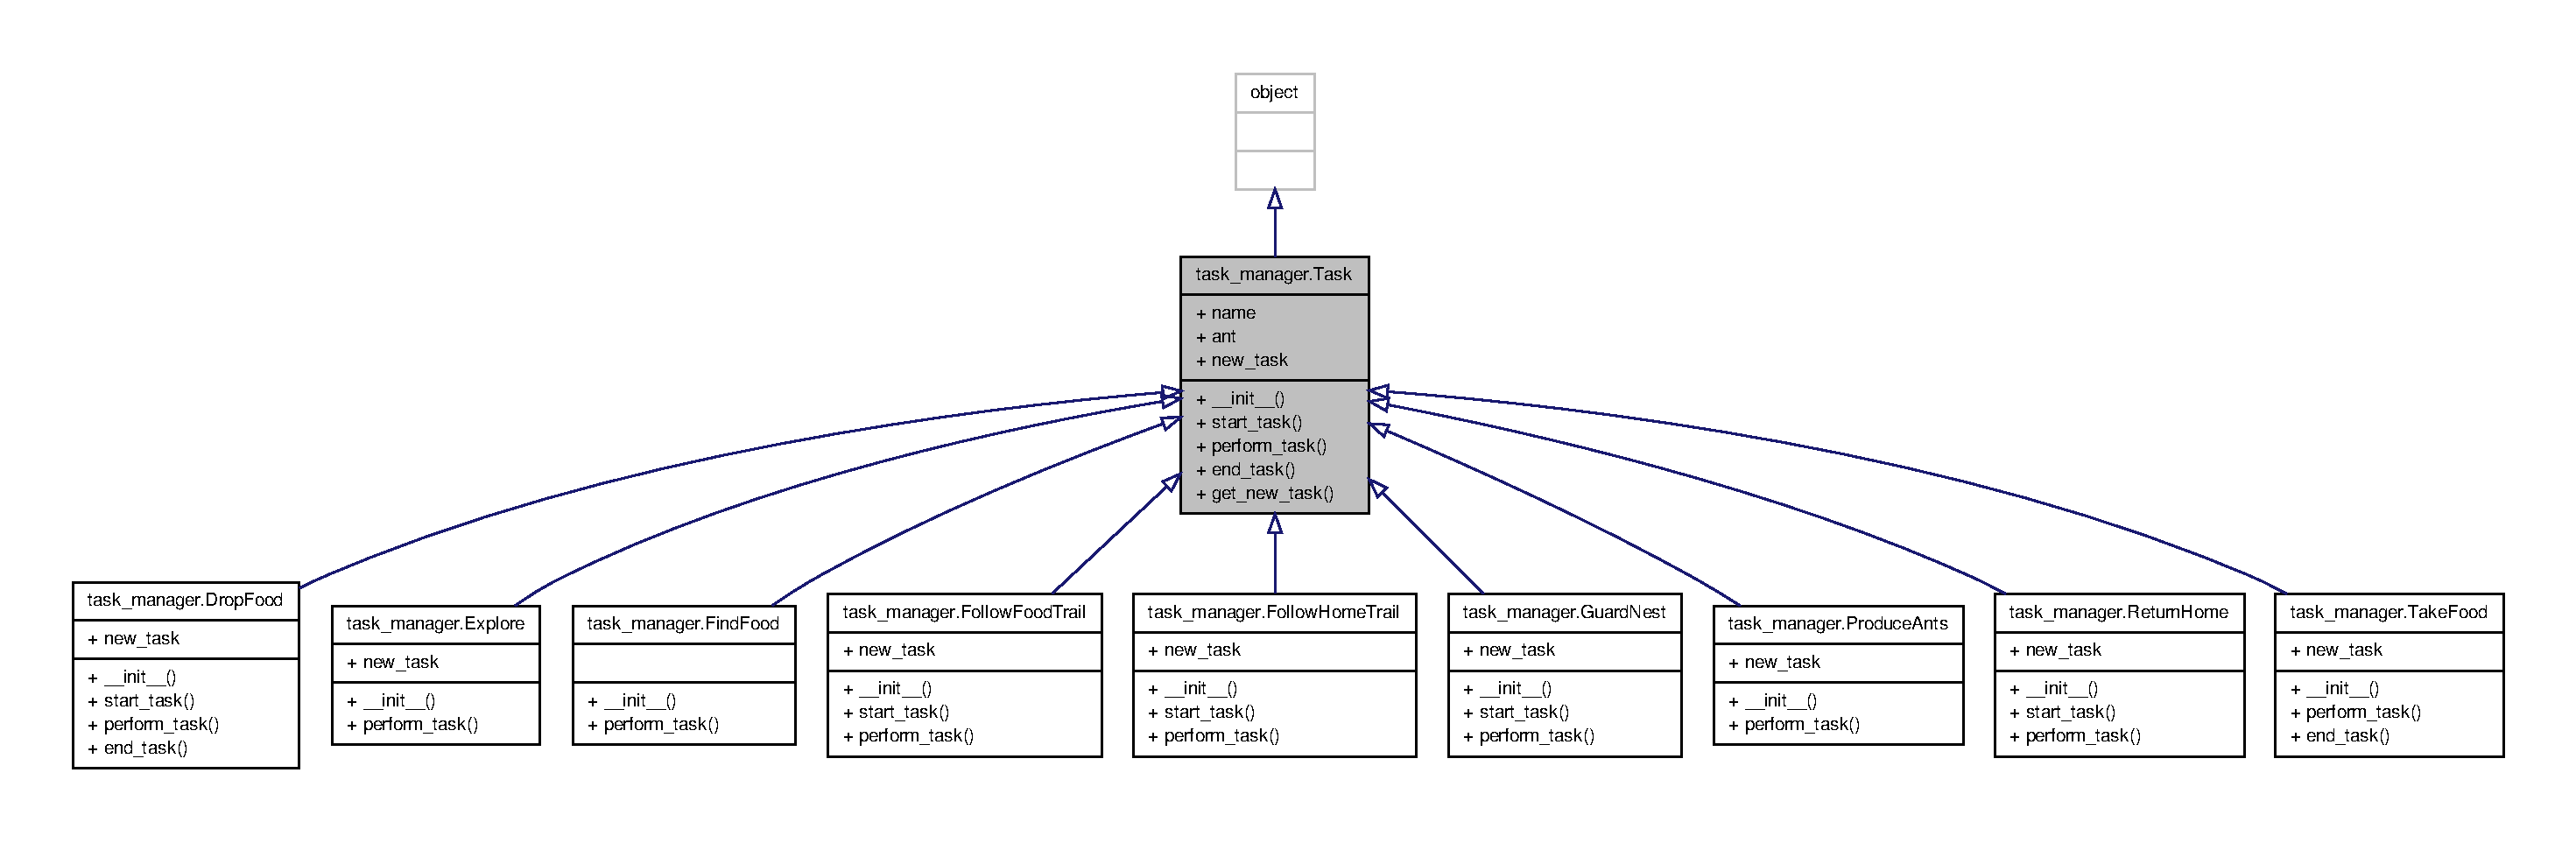
\includegraphics[width=350pt]{classtask__manager_1_1Task__inherit__graph}
\end{center}
\end{figure}


Collaboration diagram for task\+\_\+manager.\+Task\+:\nopagebreak
\begin{figure}[H]
\begin{center}
\leavevmode
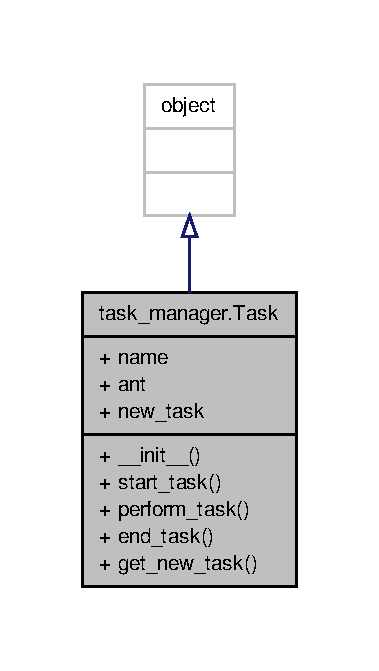
\includegraphics[width=182pt]{classtask__manager_1_1Task__coll__graph}
\end{center}
\end{figure}
\subsection*{Public Member Functions}
\begin{DoxyCompactItemize}
\item 
def \hyperlink{classtask__manager_1_1Task_aab0d2d2ec0b4b3e87969d843a101e118}{\+\_\+\+\_\+init\+\_\+\+\_\+}
\item 
def \hyperlink{classtask__manager_1_1Task_aacfcc36829c22c789f31edaf60ef1cc4}{start\+\_\+task}
\item 
def \hyperlink{classtask__manager_1_1Task_a20da98293fb7cae0c80cc0caa864c025}{perform\+\_\+task}
\item 
def \hyperlink{classtask__manager_1_1Task_a9422ddc4ca06f29aed2bbd53bfde8da4}{end\+\_\+task}
\item 
def \hyperlink{classtask__manager_1_1Task_ab46cf79945b53ec633f6f52b37c7a5cb}{get\+\_\+new\+\_\+task}
\end{DoxyCompactItemize}
\subsection*{Public Attributes}
\begin{DoxyCompactItemize}
\item 
\hyperlink{classtask__manager_1_1Task_a1a12769253144bf3a864cdff907b9fb6}{name}
\item 
\hyperlink{classtask__manager_1_1Task_ac43e25887825a1bb6e3d4a5a049968be}{ant}
\item 
\hyperlink{classtask__manager_1_1Task_af16658f4c3c447e24f73ed3d1803e058}{new\+\_\+task}
\end{DoxyCompactItemize}


\subsection{Detailed Description}
\begin{DoxyVerb}Base class for a Task\end{DoxyVerb}
 

Definition at line \hyperlink{task__manager_8py_source_l00031}{31} of file \hyperlink{task__manager_8py_source}{task\+\_\+manager.\+py}.



\subsection{Constructor \& Destructor Documentation}
\hypertarget{classtask__manager_1_1Task_aab0d2d2ec0b4b3e87969d843a101e118}{\index{task\+\_\+manager\+::\+Task@{task\+\_\+manager\+::\+Task}!\+\_\+\+\_\+init\+\_\+\+\_\+@{\+\_\+\+\_\+init\+\_\+\+\_\+}}
\index{\+\_\+\+\_\+init\+\_\+\+\_\+@{\+\_\+\+\_\+init\+\_\+\+\_\+}!task\+\_\+manager\+::\+Task@{task\+\_\+manager\+::\+Task}}
\subsubsection[{\+\_\+\+\_\+init\+\_\+\+\_\+}]{\setlength{\rightskip}{0pt plus 5cm}def task\+\_\+manager.\+Task.\+\_\+\+\_\+init\+\_\+\+\_\+ (
\begin{DoxyParamCaption}
\item[{}]{self, }
\item[{}]{name, }
\item[{}]{ant}
\end{DoxyParamCaption}
)}}\label{classtask__manager_1_1Task_aab0d2d2ec0b4b3e87969d843a101e118}


Definition at line \hyperlink{task__manager_8py_source_l00033}{33} of file \hyperlink{task__manager_8py_source}{task\+\_\+manager.\+py}.



\subsection{Member Function Documentation}
\hypertarget{classtask__manager_1_1Task_a9422ddc4ca06f29aed2bbd53bfde8da4}{\index{task\+\_\+manager\+::\+Task@{task\+\_\+manager\+::\+Task}!end\+\_\+task@{end\+\_\+task}}
\index{end\+\_\+task@{end\+\_\+task}!task\+\_\+manager\+::\+Task@{task\+\_\+manager\+::\+Task}}
\subsubsection[{end\+\_\+task}]{\setlength{\rightskip}{0pt plus 5cm}def task\+\_\+manager.\+Task.\+end\+\_\+task (
\begin{DoxyParamCaption}
\item[{}]{self}
\end{DoxyParamCaption}
)}}\label{classtask__manager_1_1Task_a9422ddc4ca06f29aed2bbd53bfde8da4}
\begin{DoxyVerb}Actions at the end of a new task\end{DoxyVerb}
 

Definition at line \hyperlink{task__manager_8py_source_l00046}{46} of file \hyperlink{task__manager_8py_source}{task\+\_\+manager.\+py}.

\hypertarget{classtask__manager_1_1Task_ab46cf79945b53ec633f6f52b37c7a5cb}{\index{task\+\_\+manager\+::\+Task@{task\+\_\+manager\+::\+Task}!get\+\_\+new\+\_\+task@{get\+\_\+new\+\_\+task}}
\index{get\+\_\+new\+\_\+task@{get\+\_\+new\+\_\+task}!task\+\_\+manager\+::\+Task@{task\+\_\+manager\+::\+Task}}
\subsubsection[{get\+\_\+new\+\_\+task}]{\setlength{\rightskip}{0pt plus 5cm}def task\+\_\+manager.\+Task.\+get\+\_\+new\+\_\+task (
\begin{DoxyParamCaption}
\item[{}]{self}
\end{DoxyParamCaption}
)}}\label{classtask__manager_1_1Task_ab46cf79945b53ec633f6f52b37c7a5cb}
\begin{DoxyVerb}Returns and resets new task\end{DoxyVerb}
 

Definition at line \hyperlink{task__manager_8py_source_l00050}{50} of file \hyperlink{task__manager_8py_source}{task\+\_\+manager.\+py}.

\hypertarget{classtask__manager_1_1Task_a20da98293fb7cae0c80cc0caa864c025}{\index{task\+\_\+manager\+::\+Task@{task\+\_\+manager\+::\+Task}!perform\+\_\+task@{perform\+\_\+task}}
\index{perform\+\_\+task@{perform\+\_\+task}!task\+\_\+manager\+::\+Task@{task\+\_\+manager\+::\+Task}}
\subsubsection[{perform\+\_\+task}]{\setlength{\rightskip}{0pt plus 5cm}def task\+\_\+manager.\+Task.\+perform\+\_\+task (
\begin{DoxyParamCaption}
\item[{}]{self}
\end{DoxyParamCaption}
)}}\label{classtask__manager_1_1Task_a20da98293fb7cae0c80cc0caa864c025}
\begin{DoxyVerb}Actions done for a task\end{DoxyVerb}
 

Definition at line \hyperlink{task__manager_8py_source_l00042}{42} of file \hyperlink{task__manager_8py_source}{task\+\_\+manager.\+py}.

\hypertarget{classtask__manager_1_1Task_aacfcc36829c22c789f31edaf60ef1cc4}{\index{task\+\_\+manager\+::\+Task@{task\+\_\+manager\+::\+Task}!start\+\_\+task@{start\+\_\+task}}
\index{start\+\_\+task@{start\+\_\+task}!task\+\_\+manager\+::\+Task@{task\+\_\+manager\+::\+Task}}
\subsubsection[{start\+\_\+task}]{\setlength{\rightskip}{0pt plus 5cm}def task\+\_\+manager.\+Task.\+start\+\_\+task (
\begin{DoxyParamCaption}
\item[{}]{self}
\end{DoxyParamCaption}
)}}\label{classtask__manager_1_1Task_aacfcc36829c22c789f31edaf60ef1cc4}
\begin{DoxyVerb}Actions at the beginning of a new task\end{DoxyVerb}
 

Definition at line \hyperlink{task__manager_8py_source_l00038}{38} of file \hyperlink{task__manager_8py_source}{task\+\_\+manager.\+py}.



\subsection{Member Data Documentation}
\hypertarget{classtask__manager_1_1Task_ac43e25887825a1bb6e3d4a5a049968be}{\index{task\+\_\+manager\+::\+Task@{task\+\_\+manager\+::\+Task}!ant@{ant}}
\index{ant@{ant}!task\+\_\+manager\+::\+Task@{task\+\_\+manager\+::\+Task}}
\subsubsection[{ant}]{\setlength{\rightskip}{0pt plus 5cm}task\+\_\+manager.\+Task.\+ant}}\label{classtask__manager_1_1Task_ac43e25887825a1bb6e3d4a5a049968be}


Definition at line \hyperlink{task__manager_8py_source_l00035}{35} of file \hyperlink{task__manager_8py_source}{task\+\_\+manager.\+py}.

\hypertarget{classtask__manager_1_1Task_a1a12769253144bf3a864cdff907b9fb6}{\index{task\+\_\+manager\+::\+Task@{task\+\_\+manager\+::\+Task}!name@{name}}
\index{name@{name}!task\+\_\+manager\+::\+Task@{task\+\_\+manager\+::\+Task}}
\subsubsection[{name}]{\setlength{\rightskip}{0pt plus 5cm}task\+\_\+manager.\+Task.\+name}}\label{classtask__manager_1_1Task_a1a12769253144bf3a864cdff907b9fb6}


Definition at line \hyperlink{task__manager_8py_source_l00034}{34} of file \hyperlink{task__manager_8py_source}{task\+\_\+manager.\+py}.

\hypertarget{classtask__manager_1_1Task_af16658f4c3c447e24f73ed3d1803e058}{\index{task\+\_\+manager\+::\+Task@{task\+\_\+manager\+::\+Task}!new\+\_\+task@{new\+\_\+task}}
\index{new\+\_\+task@{new\+\_\+task}!task\+\_\+manager\+::\+Task@{task\+\_\+manager\+::\+Task}}
\subsubsection[{new\+\_\+task}]{\setlength{\rightskip}{0pt plus 5cm}task\+\_\+manager.\+Task.\+new\+\_\+task}}\label{classtask__manager_1_1Task_af16658f4c3c447e24f73ed3d1803e058}


Definition at line \hyperlink{task__manager_8py_source_l00036}{36} of file \hyperlink{task__manager_8py_source}{task\+\_\+manager.\+py}.



The documentation for this class was generated from the following file\+:\begin{DoxyCompactItemize}
\item 
\hyperlink{task__manager_8py}{task\+\_\+manager.\+py}\end{DoxyCompactItemize}

\hypertarget{classtask__manager_1_1TaskManager}{\section{task\+\_\+manager.\+Task\+Manager Class Reference}
\label{classtask__manager_1_1TaskManager}\index{task\+\_\+manager.\+Task\+Manager@{task\+\_\+manager.\+Task\+Manager}}
}


Collaboration diagram for task\+\_\+manager.\+Task\+Manager\+:\nopagebreak
\begin{figure}[H]
\begin{center}
\leavevmode
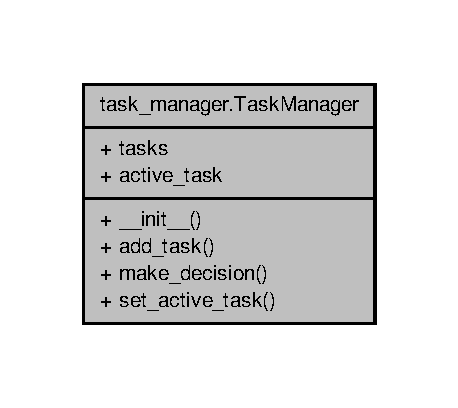
\includegraphics[width=220pt]{classtask__manager_1_1TaskManager__coll__graph}
\end{center}
\end{figure}
\subsection*{Public Member Functions}
\begin{DoxyCompactItemize}
\item 
def \hyperlink{classtask__manager_1_1TaskManager_a750d99ccae60977d027c156d607a245d}{\+\_\+\+\_\+init\+\_\+\+\_\+}
\item 
def \hyperlink{classtask__manager_1_1TaskManager_a4cedc030cbfa126c93c7050896111283}{add\+\_\+task}
\item 
def \hyperlink{classtask__manager_1_1TaskManager_a623b3d93407140ddd95753251f850f0b}{make\+\_\+decision}
\item 
def \hyperlink{classtask__manager_1_1TaskManager_ae6fddee07733c42fb3e8e29b3e45af8c}{set\+\_\+active\+\_\+task}
\end{DoxyCompactItemize}
\subsection*{Public Attributes}
\begin{DoxyCompactItemize}
\item 
\hyperlink{classtask__manager_1_1TaskManager_a13e69f2bbcef1d7ca03e92235cf9772e}{tasks}
\item 
\hyperlink{classtask__manager_1_1TaskManager_a3389ea690b2ade9bfe1efa5ad079b777}{active\+\_\+task}
\end{DoxyCompactItemize}


\subsection{Detailed Description}
\begin{DoxyVerb}Decides and performs all actions of an Ant
\end{DoxyVerb}
 

Definition at line \hyperlink{task__manager_8py_source_l00003}{3} of file \hyperlink{task__manager_8py_source}{task\+\_\+manager.\+py}.



\subsection{Constructor \& Destructor Documentation}
\hypertarget{classtask__manager_1_1TaskManager_a750d99ccae60977d027c156d607a245d}{\index{task\+\_\+manager\+::\+Task\+Manager@{task\+\_\+manager\+::\+Task\+Manager}!\+\_\+\+\_\+init\+\_\+\+\_\+@{\+\_\+\+\_\+init\+\_\+\+\_\+}}
\index{\+\_\+\+\_\+init\+\_\+\+\_\+@{\+\_\+\+\_\+init\+\_\+\+\_\+}!task\+\_\+manager\+::\+Task\+Manager@{task\+\_\+manager\+::\+Task\+Manager}}
\subsubsection[{\+\_\+\+\_\+init\+\_\+\+\_\+}]{\setlength{\rightskip}{0pt plus 5cm}def task\+\_\+manager.\+Task\+Manager.\+\_\+\+\_\+init\+\_\+\+\_\+ (
\begin{DoxyParamCaption}
\item[{}]{self}
\end{DoxyParamCaption}
)}}\label{classtask__manager_1_1TaskManager_a750d99ccae60977d027c156d607a245d}


Definition at line \hyperlink{task__manager_8py_source_l00007}{7} of file \hyperlink{task__manager_8py_source}{task\+\_\+manager.\+py}.



\subsection{Member Function Documentation}
\hypertarget{classtask__manager_1_1TaskManager_a4cedc030cbfa126c93c7050896111283}{\index{task\+\_\+manager\+::\+Task\+Manager@{task\+\_\+manager\+::\+Task\+Manager}!add\+\_\+task@{add\+\_\+task}}
\index{add\+\_\+task@{add\+\_\+task}!task\+\_\+manager\+::\+Task\+Manager@{task\+\_\+manager\+::\+Task\+Manager}}
\subsubsection[{add\+\_\+task}]{\setlength{\rightskip}{0pt plus 5cm}def task\+\_\+manager.\+Task\+Manager.\+add\+\_\+task (
\begin{DoxyParamCaption}
\item[{}]{self, }
\item[{}]{task}
\end{DoxyParamCaption}
)}}\label{classtask__manager_1_1TaskManager_a4cedc030cbfa126c93c7050896111283}
\begin{DoxyVerb}Adds a new task
\end{DoxyVerb}
 

Definition at line \hyperlink{task__manager_8py_source_l00011}{11} of file \hyperlink{task__manager_8py_source}{task\+\_\+manager.\+py}.

\hypertarget{classtask__manager_1_1TaskManager_a623b3d93407140ddd95753251f850f0b}{\index{task\+\_\+manager\+::\+Task\+Manager@{task\+\_\+manager\+::\+Task\+Manager}!make\+\_\+decision@{make\+\_\+decision}}
\index{make\+\_\+decision@{make\+\_\+decision}!task\+\_\+manager\+::\+Task\+Manager@{task\+\_\+manager\+::\+Task\+Manager}}
\subsubsection[{make\+\_\+decision}]{\setlength{\rightskip}{0pt plus 5cm}def task\+\_\+manager.\+Task\+Manager.\+make\+\_\+decision (
\begin{DoxyParamCaption}
\item[{}]{self}
\end{DoxyParamCaption}
)}}\label{classtask__manager_1_1TaskManager_a623b3d93407140ddd95753251f850f0b}
\begin{DoxyVerb}Performs the active task
Checks for new task
If new task is present end the current task and
start the new task
\end{DoxyVerb}
 

Definition at line \hyperlink{task__manager_8py_source_l00017}{17} of file \hyperlink{task__manager_8py_source}{task\+\_\+manager.\+py}.

\hypertarget{classtask__manager_1_1TaskManager_ae6fddee07733c42fb3e8e29b3e45af8c}{\index{task\+\_\+manager\+::\+Task\+Manager@{task\+\_\+manager\+::\+Task\+Manager}!set\+\_\+active\+\_\+task@{set\+\_\+active\+\_\+task}}
\index{set\+\_\+active\+\_\+task@{set\+\_\+active\+\_\+task}!task\+\_\+manager\+::\+Task\+Manager@{task\+\_\+manager\+::\+Task\+Manager}}
\subsubsection[{set\+\_\+active\+\_\+task}]{\setlength{\rightskip}{0pt plus 5cm}def task\+\_\+manager.\+Task\+Manager.\+set\+\_\+active\+\_\+task (
\begin{DoxyParamCaption}
\item[{}]{self, }
\item[{}]{task\+\_\+name}
\end{DoxyParamCaption}
)}}\label{classtask__manager_1_1TaskManager_ae6fddee07733c42fb3e8e29b3e45af8c}
\begin{DoxyVerb}Sets the active task
\end{DoxyVerb}
 

Definition at line \hyperlink{task__manager_8py_source_l00033}{33} of file \hyperlink{task__manager_8py_source}{task\+\_\+manager.\+py}.



\subsection{Member Data Documentation}
\hypertarget{classtask__manager_1_1TaskManager_a3389ea690b2ade9bfe1efa5ad079b777}{\index{task\+\_\+manager\+::\+Task\+Manager@{task\+\_\+manager\+::\+Task\+Manager}!active\+\_\+task@{active\+\_\+task}}
\index{active\+\_\+task@{active\+\_\+task}!task\+\_\+manager\+::\+Task\+Manager@{task\+\_\+manager\+::\+Task\+Manager}}
\subsubsection[{active\+\_\+task}]{\setlength{\rightskip}{0pt plus 5cm}task\+\_\+manager.\+Task\+Manager.\+active\+\_\+task}}\label{classtask__manager_1_1TaskManager_a3389ea690b2ade9bfe1efa5ad079b777}


Definition at line \hyperlink{task__manager_8py_source_l00009}{9} of file \hyperlink{task__manager_8py_source}{task\+\_\+manager.\+py}.

\hypertarget{classtask__manager_1_1TaskManager_a13e69f2bbcef1d7ca03e92235cf9772e}{\index{task\+\_\+manager\+::\+Task\+Manager@{task\+\_\+manager\+::\+Task\+Manager}!tasks@{tasks}}
\index{tasks@{tasks}!task\+\_\+manager\+::\+Task\+Manager@{task\+\_\+manager\+::\+Task\+Manager}}
\subsubsection[{tasks}]{\setlength{\rightskip}{0pt plus 5cm}task\+\_\+manager.\+Task\+Manager.\+tasks}}\label{classtask__manager_1_1TaskManager_a13e69f2bbcef1d7ca03e92235cf9772e}


Definition at line \hyperlink{task__manager_8py_source_l00008}{8} of file \hyperlink{task__manager_8py_source}{task\+\_\+manager.\+py}.



The documentation for this class was generated from the following file\+:\begin{DoxyCompactItemize}
\item 
\hyperlink{task__manager_8py}{task\+\_\+manager.\+py}\end{DoxyCompactItemize}

\hypertarget{classants_1_1WorkerAnt}{\section{ants.\+Worker\+Ant Class Reference}
\label{classants_1_1WorkerAnt}\index{ants.\+Worker\+Ant@{ants.\+Worker\+Ant}}
}


Inheritance diagram for ants.\+Worker\+Ant\+:
\nopagebreak
\begin{figure}[H]
\begin{center}
\leavevmode
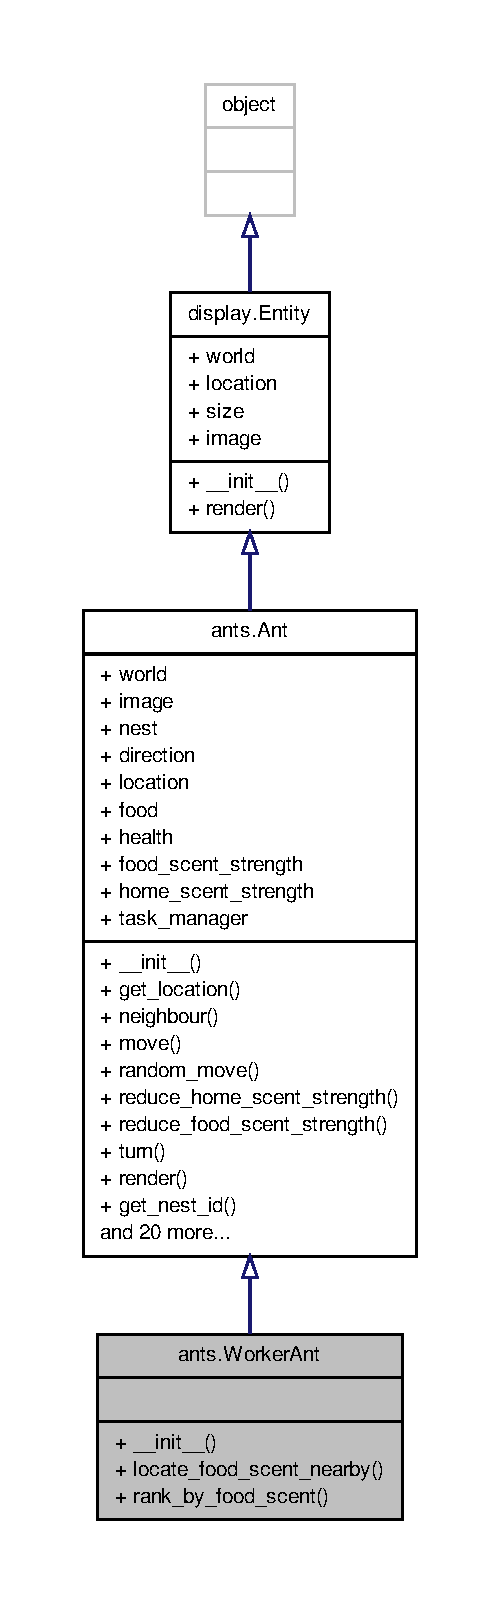
\includegraphics[height=550pt]{classants_1_1WorkerAnt__inherit__graph}
\end{center}
\end{figure}


Collaboration diagram for ants.\+Worker\+Ant\+:
\nopagebreak
\begin{figure}[H]
\begin{center}
\leavevmode
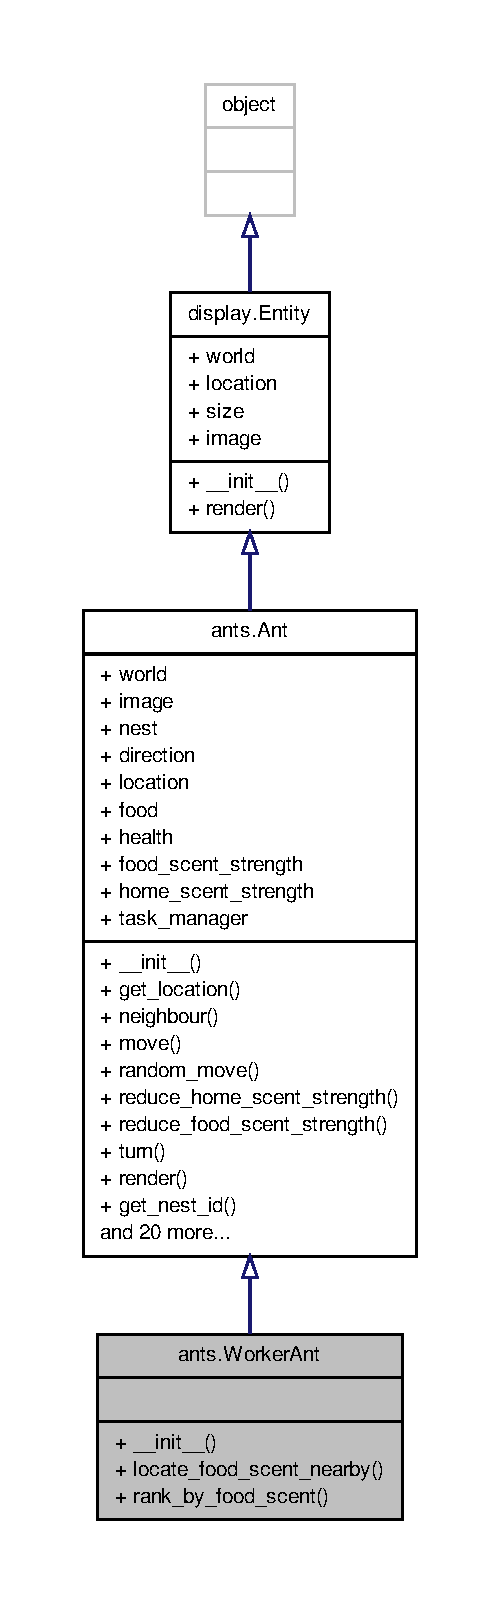
\includegraphics[height=550pt]{classants_1_1WorkerAnt__coll__graph}
\end{center}
\end{figure}
\subsection*{Public Member Functions}
\begin{DoxyCompactItemize}
\item 
def \hyperlink{classants_1_1WorkerAnt_a82e7d37f66c81e029cad6038d6515056}{\+\_\+\+\_\+init\+\_\+\+\_\+}
\end{DoxyCompactItemize}
\subsection*{Additional Inherited Members}


\subsection{Detailed Description}
\begin{DoxyVerb}Ants that explores for foodsource and collects food\end{DoxyVerb}
 

Definition at line \hyperlink{ants_8py_source_l00201}{201} of file \hyperlink{ants_8py_source}{ants.\+py}.



\subsection{Constructor \& Destructor Documentation}
\hypertarget{classants_1_1WorkerAnt_a82e7d37f66c81e029cad6038d6515056}{\index{ants\+::\+Worker\+Ant@{ants\+::\+Worker\+Ant}!\+\_\+\+\_\+init\+\_\+\+\_\+@{\+\_\+\+\_\+init\+\_\+\+\_\+}}
\index{\+\_\+\+\_\+init\+\_\+\+\_\+@{\+\_\+\+\_\+init\+\_\+\+\_\+}!ants\+::\+Worker\+Ant@{ants\+::\+Worker\+Ant}}
\subsubsection[{\+\_\+\+\_\+init\+\_\+\+\_\+}]{\setlength{\rightskip}{0pt plus 5cm}def ants.\+Worker\+Ant.\+\_\+\+\_\+init\+\_\+\+\_\+ (
\begin{DoxyParamCaption}
\item[{}]{self, }
\item[{}]{world, }
\item[{}]{image, }
\item[{}]{direction, }
\item[{}]{location}
\end{DoxyParamCaption}
)}}\label{classants_1_1WorkerAnt_a82e7d37f66c81e029cad6038d6515056}
\begin{DoxyVerb}Tasks assigned:
    - Explore
    - TakeFood
    - DropFood
    - FollowFoodTrail
    - FollowHomeTrail
Default task:
    - Explore
\end{DoxyVerb}
 

Definition at line \hyperlink{ants_8py_source_l00203}{203} of file \hyperlink{ants_8py_source}{ants.\+py}.



The documentation for this class was generated from the following file\+:\begin{DoxyCompactItemize}
\item 
\hyperlink{ants_8py}{ants.\+py}\end{DoxyCompactItemize}

\hypertarget{classworld_1_1World}{\section{world.\+World Class Reference}
\label{classworld_1_1World}\index{world.\+World@{world.\+World}}
}


Collaboration diagram for world.\+World\+:
\nopagebreak
\begin{figure}[H]
\begin{center}
\leavevmode
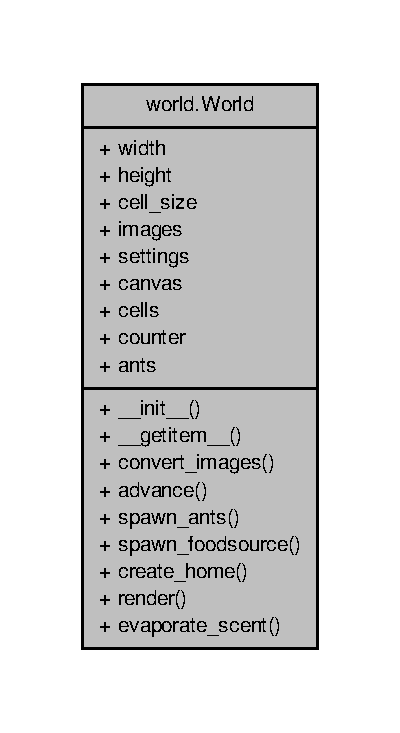
\includegraphics[width=194pt]{classworld_1_1World__coll__graph}
\end{center}
\end{figure}
\subsection*{Public Member Functions}
\begin{DoxyCompactItemize}
\item 
def \hyperlink{classworld_1_1World_a4351253668240be9d3a0d5bc2f1aa18f}{\+\_\+\+\_\+init\+\_\+\+\_\+}
\item 
def \hyperlink{classworld_1_1World_ad12e75d551845a567951b885d204153d}{\+\_\+\+\_\+getitem\+\_\+\+\_\+}
\item 
def \hyperlink{classworld_1_1World_add7ffc7d3af488f4ed006a401b842ca1}{convert\+\_\+images}
\item 
def \hyperlink{classworld_1_1World_a254dbfa03188d38b7e822c1a2e20a568}{advance}
\item 
def \hyperlink{classworld_1_1World_a83af04b7168b479b93ef75b1a9fb8dc2}{add\+\_\+ant}
\item 
def \hyperlink{classworld_1_1World_af83c041eb0a9fee93eae12bb24038b0a}{spawn\+\_\+foodsource}
\item 
def \hyperlink{classworld_1_1World_aa0e6994339219d9e933edc9bcb0c8eb5}{spawn\+\_\+colonies}
\item 
def \hyperlink{classworld_1_1World_a71b1d7a0d1b22365b4d8ed2ac6a72b98}{get\+\_\+ant\+\_\+count}
\item 
def \hyperlink{classworld_1_1World_a85d9fcbadcac5428c6f4207404221826}{create\+\_\+walls}
\item 
def \hyperlink{classworld_1_1World_a40aafbcc96e8592e314cf08068aba5f5}{render}
\item 
def \hyperlink{classworld_1_1World_a45f0825ea2f6b659d376fbc859aa208a}{evaporate\+\_\+scent}
\item 
def \hyperlink{classworld_1_1World_ad2b1f49767a4d6eae2291b1ff48c9b0d}{remove\+\_\+dead\+\_\+ants}
\end{DoxyCompactItemize}
\subsection*{Public Attributes}
\begin{DoxyCompactItemize}
\item 
\hyperlink{classworld_1_1World_a41e0f9d00bb365408abee5a084bdce24}{settings}
\item 
\hyperlink{classworld_1_1World_a5ace9de2d4cd40bbb013db9712f4ef34}{width}
\item 
\hyperlink{classworld_1_1World_acfdba03fac144372fcc56922a1a339a2}{height}
\item 
\hyperlink{classworld_1_1World_ae1d7a76e88da46ba689ac807d6a9a961}{cell\+\_\+size}
\item 
\hyperlink{classworld_1_1World_a9388f4c8146cbf9983f4a42c3015b61a}{images}
\item 
\hyperlink{classworld_1_1World_a6b3bb67973002c5018e11031462c31eb}{canvas}
\item 
\hyperlink{classworld_1_1World_a2314ff704272429f24c5d1f731ce7e8d}{cells}
\item 
\hyperlink{classworld_1_1World_a93d8708ed00be71dfd78cb42767529ce}{counter}
\item 
\hyperlink{classworld_1_1World_aff3d808329d4220a8bd5e917c151c14a}{ants}
\item 
\hyperlink{classworld_1_1World_af8524470ea81aa32b4c4045f4d5768e7}{nests}
\end{DoxyCompactItemize}


\subsection{Detailed Description}
\begin{DoxyVerb}Encapsulation of all objects in the simulation
\end{DoxyVerb}
 

Definition at line \hyperlink{world_8py_source_l00275}{275} of file \hyperlink{world_8py_source}{world.\+py}.



\subsection{Constructor \& Destructor Documentation}
\hypertarget{classworld_1_1World_a4351253668240be9d3a0d5bc2f1aa18f}{\index{world\+::\+World@{world\+::\+World}!\+\_\+\+\_\+init\+\_\+\+\_\+@{\+\_\+\+\_\+init\+\_\+\+\_\+}}
\index{\+\_\+\+\_\+init\+\_\+\+\_\+@{\+\_\+\+\_\+init\+\_\+\+\_\+}!world\+::\+World@{world\+::\+World}}
\subsubsection[{\+\_\+\+\_\+init\+\_\+\+\_\+}]{\setlength{\rightskip}{0pt plus 5cm}def world.\+World.\+\_\+\+\_\+init\+\_\+\+\_\+ (
\begin{DoxyParamCaption}
\item[{}]{self, }
\item[{}]{width, }
\item[{}]{height, }
\item[{}]{images, }
\item[{}]{settings}
\end{DoxyParamCaption}
)}}\label{classworld_1_1World_a4351253668240be9d3a0d5bc2f1aa18f}
\begin{DoxyVerb}- Initialise the screen
- Fill screen with "Cells"
- Convert images to pygame format
- Spawn ants, food sources, obstacles, ant home, etc
\end{DoxyVerb}
 

Definition at line \hyperlink{world_8py_source_l00279}{279} of file \hyperlink{world_8py_source}{world.\+py}.



\subsection{Member Function Documentation}
\hypertarget{classworld_1_1World_ad12e75d551845a567951b885d204153d}{\index{world\+::\+World@{world\+::\+World}!\+\_\+\+\_\+getitem\+\_\+\+\_\+@{\+\_\+\+\_\+getitem\+\_\+\+\_\+}}
\index{\+\_\+\+\_\+getitem\+\_\+\+\_\+@{\+\_\+\+\_\+getitem\+\_\+\+\_\+}!world\+::\+World@{world\+::\+World}}
\subsubsection[{\+\_\+\+\_\+getitem\+\_\+\+\_\+}]{\setlength{\rightskip}{0pt plus 5cm}def world.\+World.\+\_\+\+\_\+getitem\+\_\+\+\_\+ (
\begin{DoxyParamCaption}
\item[{}]{self, }
\item[{}]{location}
\end{DoxyParamCaption}
)}}\label{classworld_1_1World_ad12e75d551845a567951b885d204153d}
\begin{DoxyVerb}Returns the cell at the location
\end{DoxyVerb}
 

Definition at line \hyperlink{world_8py_source_l00309}{309} of file \hyperlink{world_8py_source}{world.\+py}.

\hypertarget{classworld_1_1World_a83af04b7168b479b93ef75b1a9fb8dc2}{\index{world\+::\+World@{world\+::\+World}!add\+\_\+ant@{add\+\_\+ant}}
\index{add\+\_\+ant@{add\+\_\+ant}!world\+::\+World@{world\+::\+World}}
\subsubsection[{add\+\_\+ant}]{\setlength{\rightskip}{0pt plus 5cm}def world.\+World.\+add\+\_\+ant (
\begin{DoxyParamCaption}
\item[{}]{self, }
\item[{}]{ant}
\end{DoxyParamCaption}
)}}\label{classworld_1_1World_a83af04b7168b479b93ef75b1a9fb8dc2}
\begin{DoxyVerb}add a new ant into the world
\end{DoxyVerb}
 

Definition at line \hyperlink{world_8py_source_l00336}{336} of file \hyperlink{world_8py_source}{world.\+py}.

\hypertarget{classworld_1_1World_a254dbfa03188d38b7e822c1a2e20a568}{\index{world\+::\+World@{world\+::\+World}!advance@{advance}}
\index{advance@{advance}!world\+::\+World@{world\+::\+World}}
\subsubsection[{advance}]{\setlength{\rightskip}{0pt plus 5cm}def world.\+World.\+advance (
\begin{DoxyParamCaption}
\item[{}]{self}
\end{DoxyParamCaption}
)}}\label{classworld_1_1World_a254dbfa03188d38b7e822c1a2e20a568}
\begin{DoxyVerb}Advance the simulation by one step
    - Update te ants
    - Evaporate all scents
\end{DoxyVerb}
 

Definition at line \hyperlink{world_8py_source_l00323}{323} of file \hyperlink{world_8py_source}{world.\+py}.

\hypertarget{classworld_1_1World_add7ffc7d3af488f4ed006a401b842ca1}{\index{world\+::\+World@{world\+::\+World}!convert\+\_\+images@{convert\+\_\+images}}
\index{convert\+\_\+images@{convert\+\_\+images}!world\+::\+World@{world\+::\+World}}
\subsubsection[{convert\+\_\+images}]{\setlength{\rightskip}{0pt plus 5cm}def world.\+World.\+convert\+\_\+images (
\begin{DoxyParamCaption}
\item[{}]{self}
\end{DoxyParamCaption}
)}}\label{classworld_1_1World_add7ffc7d3af488f4ed006a401b842ca1}
\begin{DoxyVerb}Convert images to pygame optimised format
\end{DoxyVerb}
 

Definition at line \hyperlink{world_8py_source_l00316}{316} of file \hyperlink{world_8py_source}{world.\+py}.

\hypertarget{classworld_1_1World_a85d9fcbadcac5428c6f4207404221826}{\index{world\+::\+World@{world\+::\+World}!create\+\_\+walls@{create\+\_\+walls}}
\index{create\+\_\+walls@{create\+\_\+walls}!world\+::\+World@{world\+::\+World}}
\subsubsection[{create\+\_\+walls}]{\setlength{\rightskip}{0pt plus 5cm}def world.\+World.\+create\+\_\+walls (
\begin{DoxyParamCaption}
\item[{}]{self}
\end{DoxyParamCaption}
)}}\label{classworld_1_1World_a85d9fcbadcac5428c6f4207404221826}
\begin{DoxyVerb}Generates obstacles at the edges
(otherwise the ants jump from one edge to another)
\end{DoxyVerb}
 

Definition at line \hyperlink{world_8py_source_l00377}{377} of file \hyperlink{world_8py_source}{world.\+py}.

\hypertarget{classworld_1_1World_a45f0825ea2f6b659d376fbc859aa208a}{\index{world\+::\+World@{world\+::\+World}!evaporate\+\_\+scent@{evaporate\+\_\+scent}}
\index{evaporate\+\_\+scent@{evaporate\+\_\+scent}!world\+::\+World@{world\+::\+World}}
\subsubsection[{evaporate\+\_\+scent}]{\setlength{\rightskip}{0pt plus 5cm}def world.\+World.\+evaporate\+\_\+scent (
\begin{DoxyParamCaption}
\item[{}]{self}
\end{DoxyParamCaption}
)}}\label{classworld_1_1World_a45f0825ea2f6b659d376fbc859aa208a}
\begin{DoxyVerb}Evaporates all scent ( uses decay law ) at a rate defined in settings
\end{DoxyVerb}
 

Definition at line \hyperlink{world_8py_source_l00409}{409} of file \hyperlink{world_8py_source}{world.\+py}.

\hypertarget{classworld_1_1World_a71b1d7a0d1b22365b4d8ed2ac6a72b98}{\index{world\+::\+World@{world\+::\+World}!get\+\_\+ant\+\_\+count@{get\+\_\+ant\+\_\+count}}
\index{get\+\_\+ant\+\_\+count@{get\+\_\+ant\+\_\+count}!world\+::\+World@{world\+::\+World}}
\subsubsection[{get\+\_\+ant\+\_\+count}]{\setlength{\rightskip}{0pt plus 5cm}def world.\+World.\+get\+\_\+ant\+\_\+count (
\begin{DoxyParamCaption}
\item[{}]{self}
\end{DoxyParamCaption}
)}}\label{classworld_1_1World_a71b1d7a0d1b22365b4d8ed2ac6a72b98}
\begin{DoxyVerb}Returns a list of no. of different types of ants
\end{DoxyVerb}
 

Definition at line \hyperlink{world_8py_source_l00367}{367} of file \hyperlink{world_8py_source}{world.\+py}.

\hypertarget{classworld_1_1World_ad2b1f49767a4d6eae2291b1ff48c9b0d}{\index{world\+::\+World@{world\+::\+World}!remove\+\_\+dead\+\_\+ants@{remove\+\_\+dead\+\_\+ants}}
\index{remove\+\_\+dead\+\_\+ants@{remove\+\_\+dead\+\_\+ants}!world\+::\+World@{world\+::\+World}}
\subsubsection[{remove\+\_\+dead\+\_\+ants}]{\setlength{\rightskip}{0pt plus 5cm}def world.\+World.\+remove\+\_\+dead\+\_\+ants (
\begin{DoxyParamCaption}
\item[{}]{self}
\end{DoxyParamCaption}
)}}\label{classworld_1_1World_ad2b1f49767a4d6eae2291b1ff48c9b0d}


Definition at line \hyperlink{world_8py_source_l00418}{418} of file \hyperlink{world_8py_source}{world.\+py}.

\hypertarget{classworld_1_1World_a40aafbcc96e8592e314cf08068aba5f5}{\index{world\+::\+World@{world\+::\+World}!render@{render}}
\index{render@{render}!world\+::\+World@{world\+::\+World}}
\subsubsection[{render}]{\setlength{\rightskip}{0pt plus 5cm}def world.\+World.\+render (
\begin{DoxyParamCaption}
\item[{}]{self}
\end{DoxyParamCaption}
)}}\label{classworld_1_1World_a40aafbcc96e8592e314cf08068aba5f5}
\begin{DoxyVerb}Draws the world and all its entities on the screen
\end{DoxyVerb}
 

Definition at line \hyperlink{world_8py_source_l00390}{390} of file \hyperlink{world_8py_source}{world.\+py}.

\hypertarget{classworld_1_1World_aa0e6994339219d9e933edc9bcb0c8eb5}{\index{world\+::\+World@{world\+::\+World}!spawn\+\_\+colonies@{spawn\+\_\+colonies}}
\index{spawn\+\_\+colonies@{spawn\+\_\+colonies}!world\+::\+World@{world\+::\+World}}
\subsubsection[{spawn\+\_\+colonies}]{\setlength{\rightskip}{0pt plus 5cm}def world.\+World.\+spawn\+\_\+colonies (
\begin{DoxyParamCaption}
\item[{}]{self, }
\item[{}]{n = {\ttfamily 1}}
\end{DoxyParamCaption}
)}}\label{classworld_1_1World_aa0e6994339219d9e933edc9bcb0c8eb5}
\begin{DoxyVerb}Creates colonies of ants
\end{DoxyVerb}
 

Definition at line \hyperlink{world_8py_source_l00354}{354} of file \hyperlink{world_8py_source}{world.\+py}.

\hypertarget{classworld_1_1World_af83c041eb0a9fee93eae12bb24038b0a}{\index{world\+::\+World@{world\+::\+World}!spawn\+\_\+foodsource@{spawn\+\_\+foodsource}}
\index{spawn\+\_\+foodsource@{spawn\+\_\+foodsource}!world\+::\+World@{world\+::\+World}}
\subsubsection[{spawn\+\_\+foodsource}]{\setlength{\rightskip}{0pt plus 5cm}def world.\+World.\+spawn\+\_\+foodsource (
\begin{DoxyParamCaption}
\item[{}]{self}
\end{DoxyParamCaption}
)}}\label{classworld_1_1World_af83c041eb0a9fee93eae12bb24038b0a}
\begin{DoxyVerb}Spawns food sources
\end{DoxyVerb}
 

Definition at line \hyperlink{world_8py_source_l00344}{344} of file \hyperlink{world_8py_source}{world.\+py}.



\subsection{Member Data Documentation}
\hypertarget{classworld_1_1World_aff3d808329d4220a8bd5e917c151c14a}{\index{world\+::\+World@{world\+::\+World}!ants@{ants}}
\index{ants@{ants}!world\+::\+World@{world\+::\+World}}
\subsubsection[{ants}]{\setlength{\rightskip}{0pt plus 5cm}world.\+World.\+ants}}\label{classworld_1_1World_aff3d808329d4220a8bd5e917c151c14a}


Definition at line \hyperlink{world_8py_source_l00299}{299} of file \hyperlink{world_8py_source}{world.\+py}.

\hypertarget{classworld_1_1World_a6b3bb67973002c5018e11031462c31eb}{\index{world\+::\+World@{world\+::\+World}!canvas@{canvas}}
\index{canvas@{canvas}!world\+::\+World@{world\+::\+World}}
\subsubsection[{canvas}]{\setlength{\rightskip}{0pt plus 5cm}world.\+World.\+canvas}}\label{classworld_1_1World_a6b3bb67973002c5018e11031462c31eb}


Definition at line \hyperlink{world_8py_source_l00292}{292} of file \hyperlink{world_8py_source}{world.\+py}.

\hypertarget{classworld_1_1World_ae1d7a76e88da46ba689ac807d6a9a961}{\index{world\+::\+World@{world\+::\+World}!cell\+\_\+size@{cell\+\_\+size}}
\index{cell\+\_\+size@{cell\+\_\+size}!world\+::\+World@{world\+::\+World}}
\subsubsection[{cell\+\_\+size}]{\setlength{\rightskip}{0pt plus 5cm}world.\+World.\+cell\+\_\+size}}\label{classworld_1_1World_ae1d7a76e88da46ba689ac807d6a9a961}


Definition at line \hyperlink{world_8py_source_l00289}{289} of file \hyperlink{world_8py_source}{world.\+py}.

\hypertarget{classworld_1_1World_a2314ff704272429f24c5d1f731ce7e8d}{\index{world\+::\+World@{world\+::\+World}!cells@{cells}}
\index{cells@{cells}!world\+::\+World@{world\+::\+World}}
\subsubsection[{cells}]{\setlength{\rightskip}{0pt plus 5cm}world.\+World.\+cells}}\label{classworld_1_1World_a2314ff704272429f24c5d1f731ce7e8d}


Definition at line \hyperlink{world_8py_source_l00295}{295} of file \hyperlink{world_8py_source}{world.\+py}.

\hypertarget{classworld_1_1World_a93d8708ed00be71dfd78cb42767529ce}{\index{world\+::\+World@{world\+::\+World}!counter@{counter}}
\index{counter@{counter}!world\+::\+World@{world\+::\+World}}
\subsubsection[{counter}]{\setlength{\rightskip}{0pt plus 5cm}world.\+World.\+counter}}\label{classworld_1_1World_a93d8708ed00be71dfd78cb42767529ce}


Definition at line \hyperlink{world_8py_source_l00297}{297} of file \hyperlink{world_8py_source}{world.\+py}.

\hypertarget{classworld_1_1World_acfdba03fac144372fcc56922a1a339a2}{\index{world\+::\+World@{world\+::\+World}!height@{height}}
\index{height@{height}!world\+::\+World@{world\+::\+World}}
\subsubsection[{height}]{\setlength{\rightskip}{0pt plus 5cm}world.\+World.\+height}}\label{classworld_1_1World_acfdba03fac144372fcc56922a1a339a2}


Definition at line \hyperlink{world_8py_source_l00288}{288} of file \hyperlink{world_8py_source}{world.\+py}.

\hypertarget{classworld_1_1World_a9388f4c8146cbf9983f4a42c3015b61a}{\index{world\+::\+World@{world\+::\+World}!images@{images}}
\index{images@{images}!world\+::\+World@{world\+::\+World}}
\subsubsection[{images}]{\setlength{\rightskip}{0pt plus 5cm}world.\+World.\+images}}\label{classworld_1_1World_a9388f4c8146cbf9983f4a42c3015b61a}


Definition at line \hyperlink{world_8py_source_l00290}{290} of file \hyperlink{world_8py_source}{world.\+py}.

\hypertarget{classworld_1_1World_af8524470ea81aa32b4c4045f4d5768e7}{\index{world\+::\+World@{world\+::\+World}!nests@{nests}}
\index{nests@{nests}!world\+::\+World@{world\+::\+World}}
\subsubsection[{nests}]{\setlength{\rightskip}{0pt plus 5cm}world.\+World.\+nests}}\label{classworld_1_1World_af8524470ea81aa32b4c4045f4d5768e7}


Definition at line \hyperlink{world_8py_source_l00300}{300} of file \hyperlink{world_8py_source}{world.\+py}.

\hypertarget{classworld_1_1World_a41e0f9d00bb365408abee5a084bdce24}{\index{world\+::\+World@{world\+::\+World}!settings@{settings}}
\index{settings@{settings}!world\+::\+World@{world\+::\+World}}
\subsubsection[{settings}]{\setlength{\rightskip}{0pt plus 5cm}world.\+World.\+settings}}\label{classworld_1_1World_a41e0f9d00bb365408abee5a084bdce24}


Definition at line \hyperlink{world_8py_source_l00286}{286} of file \hyperlink{world_8py_source}{world.\+py}.

\hypertarget{classworld_1_1World_a5ace9de2d4cd40bbb013db9712f4ef34}{\index{world\+::\+World@{world\+::\+World}!width@{width}}
\index{width@{width}!world\+::\+World@{world\+::\+World}}
\subsubsection[{width}]{\setlength{\rightskip}{0pt plus 5cm}world.\+World.\+width}}\label{classworld_1_1World_a5ace9de2d4cd40bbb013db9712f4ef34}


Definition at line \hyperlink{world_8py_source_l00287}{287} of file \hyperlink{world_8py_source}{world.\+py}.



The documentation for this class was generated from the following file\+:\begin{DoxyCompactItemize}
\item 
\hyperlink{world_8py}{world.\+py}\end{DoxyCompactItemize}

\chapter{File Documentation}
\hypertarget{ants_8py}{\section{ants.\+py File Reference}
\label{ants_8py}\index{ants.\+py@{ants.\+py}}
}
\subsection*{Classes}
\begin{DoxyCompactItemize}
\item 
class \hyperlink{classants_1_1Ant}{ants.\+Ant}
\item 
class \hyperlink{classants_1_1WorkerAnt}{ants.\+Worker\+Ant}
\item 
class \hyperlink{classants_1_1QueenAnt}{ants.\+Queen\+Ant}
\end{DoxyCompactItemize}
\subsection*{Namespaces}
\begin{DoxyCompactItemize}
\item 
 \hyperlink{namespaceants}{ants}
\end{DoxyCompactItemize}

\hypertarget{ants_8py_source}{\section{ants.\+py}
}

\begin{DoxyCode}
\hypertarget{ants_8py_source_l00001}{}\hyperlink{namespaceants}{00001} \textcolor{keyword}{from} constants \textcolor{keyword}{import} DIRECTIONS
00002 \textcolor{keyword}{from} task\_manager \textcolor{keyword}{import} TaskManager, Explore, TakeFood, FollowHomeTrail, FollowFoodTrail, DropFood
00003 \textcolor{keyword}{from} display \textcolor{keyword}{import} Entity
00004 \textcolor{keyword}{from} random \textcolor{keyword}{import} choice, randint
00005 
\hypertarget{ants_8py_source_l00006}{}\hyperlink{classants_1_1Ant}{00006} \textcolor{keyword}{class }\hyperlink{classants_1_1Ant}{Ant}(\hyperlink{classdisplay_1_1Entity}{Entity}):
00007     \textcolor{stringliteral}{"""A virtual base class for Ants"""}
\hypertarget{ants_8py_source_l00008}{}\hyperlink{classants_1_1Ant_a0fa15b6ba2860b445d390c07bc11d4e2}{00008}     \textcolor{keyword}{def }\hyperlink{classants_1_1Ant_a0fa15b6ba2860b445d390c07bc11d4e2}{\_\_init\_\_}(self, world, image, direction, location):
00009         super(Ant, self).\hyperlink{classants_1_1Ant_a0fa15b6ba2860b445d390c07bc11d4e2}{\_\_init\_\_}(world, location, [world.cell\_size]*2, image)
\hypertarget{ants_8py_source_l00010}{}\hyperlink{classants_1_1Ant_a55f64c7cafb3806bdcfda42586adbff5}{00010}         self.\hyperlink{classants_1_1Ant_a55f64c7cafb3806bdcfda42586adbff5}{world} = world
\hypertarget{ants_8py_source_l00011}{}\hyperlink{classants_1_1Ant_adf5f970b6b5e8472f42275114eeac779}{00011}         self.\hyperlink{classants_1_1Ant_adf5f970b6b5e8472f42275114eeac779}{image} = image
\hypertarget{ants_8py_source_l00012}{}\hyperlink{classants_1_1Ant_ae26b7ffd236a83d8d5c96ec6ec07b4bb}{00012}         self.\hyperlink{classants_1_1Ant_ae26b7ffd236a83d8d5c96ec6ec07b4bb}{direction} = direction
\hypertarget{ants_8py_source_l00013}{}\hyperlink{classants_1_1Ant_ae7de139b6f5bdb8d4ab42755c405ef5d}{00013}         self.\hyperlink{classants_1_1Ant_ae7de139b6f5bdb8d4ab42755c405ef5d}{location} = location
\hypertarget{ants_8py_source_l00014}{}\hyperlink{classants_1_1Ant_afcfbbf8bd338401378d25c512204eb91}{00014}         self.\hyperlink{classants_1_1Ant_afcfbbf8bd338401378d25c512204eb91}{food} = 0
\hypertarget{ants_8py_source_l00015}{}\hyperlink{classants_1_1Ant_ad7fb2ac4566880fdacfd7bf7f4ec1109}{00015}         self.\hyperlink{classants_1_1Ant_ad7fb2ac4566880fdacfd7bf7f4ec1109}{food\_scent\_strength} = 0
\hypertarget{ants_8py_source_l00016}{}\hyperlink{classants_1_1Ant_a7885f0124adf5b10fd6fa5e8ac47edb9}{00016}         self.\hyperlink{classants_1_1Ant_a7885f0124adf5b10fd6fa5e8ac47edb9}{home\_scent\_strength} = 0
00017 
\hypertarget{ants_8py_source_l00018}{}\hyperlink{classants_1_1Ant_a80e2218dcfabbd9ef4d83638dd20d943}{00018}         self.\hyperlink{classants_1_1Ant_a80e2218dcfabbd9ef4d83638dd20d943}{task\_manager} = \hyperlink{classtask__manager_1_1TaskManager}{TaskManager}()
00019 
\hypertarget{ants_8py_source_l00020}{}\hyperlink{classants_1_1Ant_a2ddd97dadaa5d24c459b0117dc6e1190}{00020}     \textcolor{keyword}{def }\hyperlink{classants_1_1Ant_a2ddd97dadaa5d24c459b0117dc6e1190}{neighbour}(self, direction):
00021         \textcolor{stringliteral}{"""Returns location of neighbouring cell in a direction }
00022 \textcolor{stringliteral}{        relative to the ant direction"""}
00023         x, y = self.\hyperlink{classants_1_1Ant_ae7de139b6f5bdb8d4ab42755c405ef5d}{location}
00024         dx, dy = DIRECTIONS[(self.\hyperlink{classants_1_1Ant_ae26b7ffd236a83d8d5c96ec6ec07b4bb}{direction} + direction)%8]
00025         \textcolor{keywordflow}{return} (x+dx)%self.world.width, (y+dy)%self.world.height
00026 
\hypertarget{ants_8py_source_l00027}{}\hyperlink{classants_1_1Ant_a0067159f23e5e9e4b3564d48c1564f11}{00027}     \textcolor{keyword}{def }\hyperlink{classants_1_1Ant_a0067159f23e5e9e4b3564d48c1564f11}{move}(self):
00028         \textcolor{stringliteral}{"""Move the ant by a unit,}
00029 \textcolor{stringliteral}{        Leave a scent trail,}
00030 \textcolor{stringliteral}{        remove the ant from its old cell, and}
00031 \textcolor{stringliteral}{        update the current cell ant with itself}
00032 \textcolor{stringliteral}{        """}
00033         new\_location = self.\hyperlink{classants_1_1Ant_a2ddd97dadaa5d24c459b0117dc6e1190}{neighbour}(0)       
00034         self.\hyperlink{classants_1_1Ant_ae7de139b6f5bdb8d4ab42755c405ef5d}{location} = new\_location
00035         self.\hyperlink{classants_1_1Ant_a192f8411faa05c48db8db99d033f5d15}{behind}().ant = \textcolor{keywordtype}{None}
00036         \textcolor{keywordflow}{if} \textcolor{keywordflow}{not} self.\hyperlink{classants_1_1Ant_a192f8411faa05c48db8db99d033f5d15}{behind}().is\_obstacle():
00037             self.\hyperlink{classants_1_1Ant_a192f8411faa05c48db8db99d033f5d15}{behind}().add\_home\_scent(self.\hyperlink{classants_1_1Ant_a7885f0124adf5b10fd6fa5e8ac47edb9}{home\_scent\_strength})
00038             self.\hyperlink{classants_1_1Ant_a192f8411faa05c48db8db99d033f5d15}{behind}().add\_food\_scent(self.\hyperlink{classants_1_1Ant_ad7fb2ac4566880fdacfd7bf7f4ec1109}{food\_scent\_strength}) 
00039         self.\hyperlink{classants_1_1Ant_a2e60480b7534b107e12d7f23fd06d5f1}{here}().ant = self
00040 
\hypertarget{ants_8py_source_l00041}{}\hyperlink{classants_1_1Ant_a3a636b900b6fdbed032e3a635495a4c4}{00041}     \textcolor{keyword}{def }\hyperlink{classants_1_1Ant_a3a636b900b6fdbed032e3a635495a4c4}{random\_move}(self):
00042         \textcolor{stringliteral}{"""Ant makes a move forward or turns randomly"""}
00043         \textcolor{keywordflow}{if} randint(1,8) == 1:
00044             self.\hyperlink{classants_1_1Ant_a445ec1d1f8e4cb539c4f66fafa129131}{turn}( choice([-1, 1]) )
00045         \textcolor{keywordflow}{else}:
00046             self.\hyperlink{classants_1_1Ant_a0067159f23e5e9e4b3564d48c1564f11}{move}()
00047 
\hypertarget{ants_8py_source_l00048}{}\hyperlink{classants_1_1Ant_a216ebc2ce2dfeb88d6bbc714bc50ecb5}{00048}     \textcolor{keyword}{def }\hyperlink{classants_1_1Ant_a216ebc2ce2dfeb88d6bbc714bc50ecb5}{reduce\_home\_scent}(self, amt=1):
00049         \textcolor{stringliteral}{"""Reduce home scent by 'amt'"""}
00050         self.\hyperlink{classants_1_1Ant_a7885f0124adf5b10fd6fa5e8ac47edb9}{home\_scent\_strength} = max(0, self.
      \hyperlink{classants_1_1Ant_a7885f0124adf5b10fd6fa5e8ac47edb9}{home\_scent\_strength}-amt)
00051         \textcolor{keywordflow}{return} self
00052 
\hypertarget{ants_8py_source_l00053}{}\hyperlink{classants_1_1Ant_a285d1e406b6d2cc67779e873e879feb0}{00053}     \textcolor{keyword}{def }\hyperlink{classants_1_1Ant_a285d1e406b6d2cc67779e873e879feb0}{reduce\_food\_scent}(self, amt=1):
00054         \textcolor{stringliteral}{"""Reduce food scent by 'amt'"""}
00055         self.\hyperlink{classants_1_1Ant_ad7fb2ac4566880fdacfd7bf7f4ec1109}{food\_scent\_strength} = max(0, self.
      \hyperlink{classants_1_1Ant_ad7fb2ac4566880fdacfd7bf7f4ec1109}{food\_scent\_strength}-amt)
00056         \textcolor{keywordflow}{return} self
00057 
\hypertarget{ants_8py_source_l00058}{}\hyperlink{classants_1_1Ant_a445ec1d1f8e4cb539c4f66fafa129131}{00058}     \textcolor{keyword}{def }\hyperlink{classants_1_1Ant_a445ec1d1f8e4cb539c4f66fafa129131}{turn}(self, n):
00059         \textcolor{stringliteral}{"""Changes direction n times"""}
00060         self.\hyperlink{classants_1_1Ant_ae26b7ffd236a83d8d5c96ec6ec07b4bb}{direction} = (self.\hyperlink{classants_1_1Ant_ae26b7ffd236a83d8d5c96ec6ec07b4bb}{direction} + n) % 8
00061 
\hypertarget{ants_8py_source_l00062}{}\hyperlink{classants_1_1Ant_a95585d833c74c56155a0d79394d511cc}{00062}     \textcolor{keyword}{def }\hyperlink{classants_1_1Ant_a95585d833c74c56155a0d79394d511cc}{render}(self):
00063         \textcolor{stringliteral}{"""Render itself"""}
00064         \textcolor{keywordflow}{if} self.\hyperlink{classants_1_1Ant_a41de1c29941a444dab25a88cbc3a881d}{has\_food}():
00065             super(Ant, self).\hyperlink{classants_1_1Ant_a95585d833c74c56155a0d79394d511cc}{render}(8)
00066         \textcolor{keywordflow}{else}:
00067             super(Ant, self).\hyperlink{classants_1_1Ant_a95585d833c74c56155a0d79394d511cc}{render}(self.\hyperlink{classants_1_1Ant_ae26b7ffd236a83d8d5c96ec6ec07b4bb}{direction})
00068 
\hypertarget{ants_8py_source_l00069}{}\hyperlink{classants_1_1Ant_a2e60480b7534b107e12d7f23fd06d5f1}{00069}     \textcolor{keyword}{def }\hyperlink{classants_1_1Ant_a2e60480b7534b107e12d7f23fd06d5f1}{here}(self):
00070         \textcolor{stringliteral}{"""The cell it is standing on"""}
00071         \textcolor{keywordflow}{return} self.\hyperlink{classants_1_1Ant_a55f64c7cafb3806bdcfda42586adbff5}{world}[self.\hyperlink{classants_1_1Ant_ae7de139b6f5bdb8d4ab42755c405ef5d}{location}]
00072 
\hypertarget{ants_8py_source_l00073}{}\hyperlink{classants_1_1Ant_a192f8411faa05c48db8db99d033f5d15}{00073}     \textcolor{keyword}{def }\hyperlink{classants_1_1Ant_a192f8411faa05c48db8db99d033f5d15}{behind}(self):
00074         \textcolor{stringliteral}{"""The cell just behind"""}
00075         \textcolor{keywordflow}{return} self.\hyperlink{classants_1_1Ant_a55f64c7cafb3806bdcfda42586adbff5}{world}[self.\hyperlink{classants_1_1Ant_a2ddd97dadaa5d24c459b0117dc6e1190}{neighbour}(4)]
00076 
\hypertarget{ants_8py_source_l00077}{}\hyperlink{classants_1_1Ant_ac2c8f048d99cd48a5829ddf7ff4a708a}{00077}     \textcolor{keyword}{def }\hyperlink{classants_1_1Ant_ac2c8f048d99cd48a5829ddf7ff4a708a}{ahead}(self):
00078         \textcolor{stringliteral}{"""The cell just ahead"""}
00079         \textcolor{keywordflow}{return} self.\hyperlink{classants_1_1Ant_a55f64c7cafb3806bdcfda42586adbff5}{world}[self.\hyperlink{classants_1_1Ant_a2ddd97dadaa5d24c459b0117dc6e1190}{neighbour}(0)]
00080 
\hypertarget{ants_8py_source_l00081}{}\hyperlink{classants_1_1Ant_a2dbb07eefeecbc51d257f81fb0ba1c71}{00081}     \textcolor{keyword}{def }\hyperlink{classants_1_1Ant_a2dbb07eefeecbc51d257f81fb0ba1c71}{ahead\_left}(self):
00082         \textcolor{stringliteral}{"""The cell just ahead-left"""}
00083         \textcolor{keywordflow}{return} self.\hyperlink{classants_1_1Ant_a55f64c7cafb3806bdcfda42586adbff5}{world}[self.\hyperlink{classants_1_1Ant_a2ddd97dadaa5d24c459b0117dc6e1190}{neighbour}(-1)]
00084 
\hypertarget{ants_8py_source_l00085}{}\hyperlink{classants_1_1Ant_ad7a5311d831e8bcc07061e6a12edad8c}{00085}     \textcolor{keyword}{def }\hyperlink{classants_1_1Ant_ad7a5311d831e8bcc07061e6a12edad8c}{ahead\_right}(self):
00086         \textcolor{stringliteral}{"""The cell just ahead-right"""}
00087         \textcolor{keywordflow}{return} self.\hyperlink{classants_1_1Ant_a55f64c7cafb3806bdcfda42586adbff5}{world}[self.\hyperlink{classants_1_1Ant_a2ddd97dadaa5d24c459b0117dc6e1190}{neighbour}(1)]
00088 
\hypertarget{ants_8py_source_l00089}{}\hyperlink{classants_1_1Ant_af9af7f8a5c766021ef0f68171d09abca}{00089}     \textcolor{keyword}{def }\hyperlink{classants_1_1Ant_af9af7f8a5c766021ef0f68171d09abca}{locate\_food\_nearby}(self):
00090         \textcolor{stringliteral}{"""Locate all sources nearby and return any one randomly}
00091 \textcolor{stringliteral}{        return None if no food source is found"""}
00092         directions = []
00093         \textcolor{keywordflow}{if} self.\hyperlink{classants_1_1Ant_ac2c8f048d99cd48a5829ddf7ff4a708a}{ahead}().\hyperlink{classants_1_1Ant_a41de1c29941a444dab25a88cbc3a881d}{has\_food}():
00094             directions.append(0)
00095         \textcolor{keywordflow}{else}:
00096             \textcolor{keywordflow}{for} i \textcolor{keywordflow}{in} xrange(1, 8):
00097                 \textcolor{keywordflow}{if} self.\hyperlink{classants_1_1Ant_a55f64c7cafb3806bdcfda42586adbff5}{world}[self.\hyperlink{classants_1_1Ant_a2ddd97dadaa5d24c459b0117dc6e1190}{neighbour}(i)].\hyperlink{classants_1_1Ant_a41de1c29941a444dab25a88cbc3a881d}{has\_food}():
00098                     directions.append(i) 
00099 
00100         \textcolor{keywordflow}{if} directions:
00101             \textcolor{keywordflow}{return} choice(directions)
00102         \textcolor{keywordflow}{else}:
00103             \textcolor{keywordflow}{return} \textcolor{keywordtype}{None}
00104 
\hypertarget{ants_8py_source_l00105}{}\hyperlink{classants_1_1Ant_a5795d0898e3d0d020a0a0a626a5ef7b0}{00105}     \textcolor{keyword}{def }\hyperlink{classants_1_1Ant_a5795d0898e3d0d020a0a0a626a5ef7b0}{locate\_home\_nearby}(self):
00106         \textcolor{stringliteral}{"""Locate home cell nearby and return any one randomly}
00107 \textcolor{stringliteral}{        return None if not found"""}
00108         directions = []
00109         \textcolor{keywordflow}{if} self.\hyperlink{classants_1_1Ant_ac2c8f048d99cd48a5829ddf7ff4a708a}{ahead}().is\_food():
00110             directions.append(0)
00111         \textcolor{keywordflow}{else}:
00112             \textcolor{keywordflow}{for} i \textcolor{keywordflow}{in} xrange(1, 8):
00113                 \textcolor{keywordflow}{if} self.\hyperlink{classants_1_1Ant_a55f64c7cafb3806bdcfda42586adbff5}{world}[self.\hyperlink{classants_1_1Ant_a2ddd97dadaa5d24c459b0117dc6e1190}{neighbour}(i)].is\_home():
00114                     directions.append(i) 
00115 
00116         \textcolor{keywordflow}{if} directions:
00117             \textcolor{keywordflow}{return} choice(directions)
00118         \textcolor{keywordflow}{else}:
00119             \textcolor{keywordflow}{return} \textcolor{keywordtype}{None}
00120 
\hypertarget{ants_8py_source_l00121}{}\hyperlink{classants_1_1Ant_a81a141f3417ddb32b8d1abbd95bbc477}{00121}     \textcolor{keyword}{def }\hyperlink{classants_1_1Ant_a81a141f3417ddb32b8d1abbd95bbc477}{locate\_home\_scent\_nearby}(self):
00122         \textcolor{stringliteral}{"""Scan the 5 directions near the direction of the ant for home scent and}
00123 \textcolor{stringliteral}{        return one random direction}
00124 \textcolor{stringliteral}{        return None if not found}
00125 \textcolor{stringliteral}{        """}
00126         directions = []
00127         \textcolor{keywordflow}{if} self.\hyperlink{classants_1_1Ant_ac2c8f048d99cd48a5829ddf7ff4a708a}{ahead}().home\_scent > 0:
00128             directions.append(0)
00129         \textcolor{keywordflow}{else}:
00130             \textcolor{keywordflow}{for} i \textcolor{keywordflow}{in} xrange(-2, 3):
00131                 \textcolor{keywordflow}{if} self.\hyperlink{classants_1_1Ant_a55f64c7cafb3806bdcfda42586adbff5}{world}[self.\hyperlink{classants_1_1Ant_a2ddd97dadaa5d24c459b0117dc6e1190}{neighbour}(i)].home\_scent > 0:
00132                     \textcolor{keywordflow}{for} x \textcolor{keywordflow}{in} xrange(1,11-5*abs(i)):
00133                         directions.append(i) 
00134 
00135         \textcolor{keywordflow}{if} directions:
00136             \textcolor{keywordflow}{return} choice(directions)
00137         \textcolor{keywordflow}{else}:
00138             \textcolor{keywordflow}{return} \textcolor{keywordtype}{None}
00139 
\hypertarget{ants_8py_source_l00140}{}\hyperlink{classants_1_1Ant_a97ffad1c0e634f38585e7913908e9524}{00140}     \textcolor{keyword}{def }\hyperlink{classants_1_1Ant_a97ffad1c0e634f38585e7913908e9524}{locate\_food\_scent\_nearby}(self):
00141         \textcolor{stringliteral}{"""Scan the 5 directions near the direction of the ant for food scent and}
00142 \textcolor{stringliteral}{        return one random direction}
00143 \textcolor{stringliteral}{        return None if not found}
00144 \textcolor{stringliteral}{        """}
00145         directions = []
00146         \textcolor{keywordflow}{if} self.\hyperlink{classants_1_1Ant_ac2c8f048d99cd48a5829ddf7ff4a708a}{ahead}().food\_scent > 0:
00147             directions.append(0)
00148         \textcolor{keywordflow}{else}:
00149             \textcolor{keywordflow}{for} i \textcolor{keywordflow}{in} xrange(-2, 3):
00150                 \textcolor{keywordflow}{if} self.\hyperlink{classants_1_1Ant_a55f64c7cafb3806bdcfda42586adbff5}{world}[self.\hyperlink{classants_1_1Ant_a2ddd97dadaa5d24c459b0117dc6e1190}{neighbour}(i)].food\_scent > 0:
00151                     \textcolor{keywordflow}{for} x \textcolor{keywordflow}{in} xrange(1,11-5*abs(i)):
00152                         directions.append(i) 
00153 
00154         \textcolor{keywordflow}{if} directions:
00155             \textcolor{keywordflow}{return} choice(directions)
00156         \textcolor{keywordflow}{else}:
00157             \textcolor{keywordflow}{return} \textcolor{keywordtype}{None}
00158 
\hypertarget{ants_8py_source_l00159}{}\hyperlink{classants_1_1Ant_a164a2a76f1779462fe81e8f169a92a93}{00159}     \textcolor{keyword}{def }\hyperlink{classants_1_1Ant_a164a2a76f1779462fe81e8f169a92a93}{rank\_by\_food\_scent}(self):
00160         \textcolor{stringliteral}{"""Scan the 5 directions near the direction of the ant for food scent and}
00161 \textcolor{stringliteral}{        return the direction with the strongest scent}
00162 \textcolor{stringliteral}{        return None if not found}
00163 \textcolor{stringliteral}{        """}
00164         best\_direction = 0
00165         best\_direction\_scent = 0
00166         \textcolor{keywordflow}{for} i \textcolor{keywordflow}{in} [0, -1, 1, -1, 2]:
00167             cell = self.\hyperlink{classants_1_1Ant_a55f64c7cafb3806bdcfda42586adbff5}{world}[self.\hyperlink{classants_1_1Ant_a2ddd97dadaa5d24c459b0117dc6e1190}{neighbour}(i)]
00168             \textcolor{keywordflow}{if} cell.food\_scent > best\_direction\_scent:
00169                 best\_direction = i
00170                 best\_direction\_scent = cell.food\_scent
00171         \textcolor{keywordflow}{return} best\_direction
00172 
\hypertarget{ants_8py_source_l00173}{}\hyperlink{classants_1_1Ant_a6f3e3bd98a5f382098cdc1c02e1e2fd0}{00173}     \textcolor{keyword}{def }\hyperlink{classants_1_1Ant_a6f3e3bd98a5f382098cdc1c02e1e2fd0}{rank\_by\_home\_scent}(self):
00174         \textcolor{stringliteral}{"""Scan the 5 directions near the direction of the ant for home scent and}
00175 \textcolor{stringliteral}{        return the direction with the strongest scent}
00176 \textcolor{stringliteral}{        return None if not found}
00177 \textcolor{stringliteral}{        """}
00178         best\_direction = 0
00179         best\_direction\_scent = 0
00180         \textcolor{keywordflow}{for} i \textcolor{keywordflow}{in} [0, -1, 1, -1, 2]:
00181             cell = self.\hyperlink{classants_1_1Ant_a55f64c7cafb3806bdcfda42586adbff5}{world}[self.\hyperlink{classants_1_1Ant_a2ddd97dadaa5d24c459b0117dc6e1190}{neighbour}(i)]
00182             \textcolor{keywordflow}{if} cell.home\_scent > best\_direction\_scent:
00183                 best\_direction = i
00184                 best\_direction\_scent = cell.home\_scent
00185         \textcolor{keywordflow}{return} best\_direction
00186 
\hypertarget{ants_8py_source_l00187}{}\hyperlink{classants_1_1Ant_ae85884312b4aa10f965b84535bed37fc}{00187}     \textcolor{keyword}{def }\hyperlink{classants_1_1Ant_ae85884312b4aa10f965b84535bed37fc}{drop\_food}(self):
00188         \textcolor{stringliteral}{"""}
00189 \textcolor{stringliteral}{        Set food to zero}
00190 \textcolor{stringliteral}{        Update the food values of the home cell it reached}
00191 \textcolor{stringliteral}{        """}
00192         self.\hyperlink{classants_1_1Ant_afcfbbf8bd338401378d25c512204eb91}{food} = 0
00193 
\hypertarget{ants_8py_source_l00194}{}\hyperlink{classants_1_1Ant_a41de1c29941a444dab25a88cbc3a881d}{00194}     \textcolor{keyword}{def }\hyperlink{classants_1_1Ant_a41de1c29941a444dab25a88cbc3a881d}{has\_food}(self):
00195         \textcolor{keywordflow}{return} bool(self.\hyperlink{classants_1_1Ant_afcfbbf8bd338401378d25c512204eb91}{food})
00196 
\hypertarget{ants_8py_source_l00197}{}\hyperlink{classants_1_1Ant_a9e4bf6309b80ab33bd628f6e7d78d013}{00197}     \textcolor{keyword}{def }\hyperlink{classants_1_1Ant_a9e4bf6309b80ab33bd628f6e7d78d013}{\_\_nonzero\_\_}(self):
00198         \textcolor{keywordflow}{return} \textcolor{keyword}{True}
00199 
00200 
\hypertarget{ants_8py_source_l00201}{}\hyperlink{classants_1_1WorkerAnt}{00201} \textcolor{keyword}{class }\hyperlink{classants_1_1WorkerAnt}{WorkerAnt}(\hyperlink{classants_1_1Ant}{Ant}):
00202     \textcolor{stringliteral}{"""Ants that explores for foodsource and collects food"""}
\hypertarget{ants_8py_source_l00203}{}\hyperlink{classants_1_1WorkerAnt_a82e7d37f66c81e029cad6038d6515056}{00203}     \textcolor{keyword}{def }\hyperlink{classants_1_1WorkerAnt_a82e7d37f66c81e029cad6038d6515056}{\_\_init\_\_}(self, world, image, direction, location):
00204         \textcolor{stringliteral}{"""}
00205 \textcolor{stringliteral}{        Tasks assigned:}
00206 \textcolor{stringliteral}{            - Explore}
00207 \textcolor{stringliteral}{            - TakeFood}
00208 \textcolor{stringliteral}{            - DropFood}
00209 \textcolor{stringliteral}{            - FollowFoodTrail}
00210 \textcolor{stringliteral}{            - FollowHomeTrail}
00211 \textcolor{stringliteral}{        Default task:}
00212 \textcolor{stringliteral}{            - Explore}
00213 \textcolor{stringliteral}{        """}
00214         Ant.\_\_init\_\_(self, world, image, direction, location)
00215         self.task\_manager.add\_task(\hyperlink{classtask__manager_1_1Explore}{Explore}(self))
00216         self.task\_manager.add\_task(\hyperlink{classtask__manager_1_1TakeFood}{TakeFood}(self))
00217         self.task\_manager.add\_task(\hyperlink{classtask__manager_1_1DropFood}{DropFood}(self))
00218         self.task\_manager.add\_task(\hyperlink{classtask__manager_1_1FollowFoodTrail}{FollowFoodTrail}(self))
00219         self.task\_manager.add\_task(\hyperlink{classtask__manager_1_1FollowHomeTrail}{FollowHomeTrail}(self))
00220         self.task\_manager.set\_active\_task(\textcolor{stringliteral}{"explore"})
00221 
00222 
\hypertarget{ants_8py_source_l00223}{}\hyperlink{classants_1_1QueenAnt}{00223} \textcolor{keyword}{class }\hyperlink{classants_1_1QueenAnt}{QueenAnt}(\hyperlink{classants_1_1Ant}{Ant}):
00224     \textcolor{stringliteral}{"""Ants that produces offsprings and populates the colony"""}
\hypertarget{ants_8py_source_l00225}{}\hyperlink{classants_1_1QueenAnt_aea3ff8fa90122567905806f675eb9472}{00225}     \textcolor{keyword}{def }\hyperlink{classants_1_1QueenAnt_aea3ff8fa90122567905806f675eb9472}{\_\_init\_\_}(self, world, image, direction, location):
00226         \textcolor{stringliteral}{"""}
00227 \textcolor{stringliteral}{        Tasks assigned:}
00228 \textcolor{stringliteral}{            - HaveFood}
00229 \textcolor{stringliteral}{            - Produce offsprings}
00230 \textcolor{stringliteral}{        Default task:}
00231 \textcolor{stringliteral}{            - Have Food}
00232 \textcolor{stringliteral}{        """}
00233         Ant.\_\_init\_\_(self, world, image, direction, location)
00234         \textcolor{keywordflow}{raise} NotImplementedError
\end{DoxyCode}

\hypertarget{constants_8py}{\section{constants.\+py File Reference}
\label{constants_8py}\index{constants.\+py@{constants.\+py}}
}
\subsection*{Namespaces}
\begin{DoxyCompactItemize}
\item 
 \hyperlink{namespaceconstants}{constants}
\end{DoxyCompactItemize}
\subsection*{Variables}
\begin{DoxyCompactItemize}
\item 
tuple \hyperlink{namespaceconstants_ac910045b50610ec197515a3635d8d037}{constants.\+D\+I\+R\+E\+C\+T\+I\+O\+N\+S}
\item 
int \hyperlink{namespaceconstants_aa1f49ae50d4547cd3b9f4801d04f5830}{constants.\+W\+I\+D\+T\+H} = 80
\item 
int \hyperlink{namespaceconstants_a581305cb095bf2d8826a12abef66a15e}{constants.\+H\+E\+I\+G\+H\+T} = 60
\end{DoxyCompactItemize}

\hypertarget{constants_8py_source}{\section{constants.\+py}
}

\begin{DoxyCode}
\hypertarget{constants_8py_source_l00001}{}\hyperlink{namespaceconstants_ac910045b50610ec197515a3635d8d037}{00001} DIRECTIONS = ((1,0), (1,1), (0,1), (-1,1),
00002     (-1,0), (-1,-1), (0,-1), (1,-1))
\hypertarget{constants_8py_source_l00003}{}\hyperlink{namespaceconstants_aa1f49ae50d4547cd3b9f4801d04f5830}{00003} WIDTH = 80
\hypertarget{constants_8py_source_l00004}{}\hyperlink{namespaceconstants_a581305cb095bf2d8826a12abef66a15e}{00004} HEIGHT = 60
00005 WHITE = (255,255,255)
\end{DoxyCode}

\hypertarget{controller_8py}{\section{controller.\+py File Reference}
\label{controller_8py}\index{controller.\+py@{controller.\+py}}
}
\subsection*{Classes}
\begin{DoxyCompactItemize}
\item 
class \hyperlink{classcontroller_1_1Simulation}{controller.\+Simulation}
\end{DoxyCompactItemize}
\subsection*{Namespaces}
\begin{DoxyCompactItemize}
\item 
 \hyperlink{namespacecontroller}{controller}
\end{DoxyCompactItemize}

\hypertarget{controller_8py_source}{\section{controller.\+py}
}

\begin{DoxyCode}
\hypertarget{controller_8py_source_l00001}{}\hyperlink{namespacecontroller}{00001} \textcolor{keyword}{from} pygame \textcolor{keyword}{import} image, time, key, event
00002 \textcolor{keyword}{from} \hyperlink{namespacepygame_1_1constants}{pygame.constants} \textcolor{keyword}{import} *
00003 \textcolor{keyword}{from} world \textcolor{keyword}{import} World
00004 
\hypertarget{controller_8py_source_l00005}{}\hyperlink{classcontroller_1_1Simulation}{00005} \textcolor{keyword}{class }\hyperlink{classcontroller_1_1Simulation}{Simulation}():
00006     \textcolor{stringliteral}{"""Controls the simulation}
00007 \textcolor{stringliteral}{}
00008 \textcolor{stringliteral}{        - Runs the main loop}
00009 \textcolor{stringliteral}{        - Detects mouse, keyboard and other events}
00010 \textcolor{stringliteral}{        - Loads the necessary images}
00011 \textcolor{stringliteral}{        - Controls the framerate of the smiulation}
00012 \textcolor{stringliteral}{    """}
\hypertarget{controller_8py_source_l00013}{}\hyperlink{classcontroller_1_1Simulation_a0d3a98e6f630a62f18aa5c0c35846381}{00013}     \textcolor{keyword}{def }\hyperlink{classcontroller_1_1Simulation_a0d3a98e6f630a62f18aa5c0c35846381}{\_\_init\_\_}(self):
\hypertarget{controller_8py_source_l00014}{}\hyperlink{classcontroller_1_1Simulation_a21dd9474d46d4afa868c0bd60cea128b}{00014}         self.\hyperlink{classcontroller_1_1Simulation_a21dd9474d46d4afa868c0bd60cea128b}{clock} = time.Clock()
\hypertarget{controller_8py_source_l00015}{}\hyperlink{classcontroller_1_1Simulation_a2bc2a4bb3e974bc7b73be75b49701d9f}{00015}         self.\hyperlink{classcontroller_1_1Simulation_a2bc2a4bb3e974bc7b73be75b49701d9f}{framerate} = 60
\hypertarget{controller_8py_source_l00016}{}\hyperlink{classcontroller_1_1Simulation_af13461f42bfe6ca017f59e13e57c354e}{00016}         self.\hyperlink{classcontroller_1_1Simulation_af13461f42bfe6ca017f59e13e57c354e}{images} = \{\}
00017 
\hypertarget{controller_8py_source_l00018}{}\hyperlink{classcontroller_1_1Simulation_a35d0ffc695295c3b509bd5bc2bdbac9b}{00018}         self.\hyperlink{classcontroller_1_1Simulation_a35d0ffc695295c3b509bd5bc2bdbac9b}{quit} = \textcolor{keyword}{False}
00019 
00020         self.\hyperlink{classcontroller_1_1Simulation_a91674f018c921725aa36ec25396a7304}{add\_image}(\textcolor{stringliteral}{"ant"}, \textcolor{stringliteral}{"ant.png"})
00021         self.\hyperlink{classcontroller_1_1Simulation_a91674f018c921725aa36ec25396a7304}{add\_image}(\textcolor{stringliteral}{"grass"}, \textcolor{stringliteral}{"grass.png"})
00022         self.\hyperlink{classcontroller_1_1Simulation_a91674f018c921725aa36ec25396a7304}{add\_image}(\textcolor{stringliteral}{"food"}, \textcolor{stringliteral}{"food.png"})
00023         self.\hyperlink{classcontroller_1_1Simulation_a91674f018c921725aa36ec25396a7304}{add\_image}(\textcolor{stringliteral}{"home"}, \textcolor{stringliteral}{"home.png"})
00024         self.\hyperlink{classcontroller_1_1Simulation_a91674f018c921725aa36ec25396a7304}{add\_image}(\textcolor{stringliteral}{"obstacle"}, \textcolor{stringliteral}{"obstacle.png"})
00025         self.\hyperlink{classcontroller_1_1Simulation_a91674f018c921725aa36ec25396a7304}{add\_image}(\textcolor{stringliteral}{"home\_scent"}, \textcolor{stringliteral}{"home\_scent.png"})
00026         self.\hyperlink{classcontroller_1_1Simulation_a91674f018c921725aa36ec25396a7304}{add\_image}(\textcolor{stringliteral}{"food\_scent"}, \textcolor{stringliteral}{"food\_scent.png"})
00027         self.\hyperlink{classcontroller_1_1Simulation_a91674f018c921725aa36ec25396a7304}{add\_image}(\textcolor{stringliteral}{"cell"}, \textcolor{stringliteral}{"cell.png"})
00028 
\hypertarget{controller_8py_source_l00029}{}\hyperlink{classcontroller_1_1Simulation_a5d368ffc3eee12c8c36839ee5bce3644}{00029}         self.\hyperlink{classcontroller_1_1Simulation_a5d368ffc3eee12c8c36839ee5bce3644}{settings} = \{
00030         \textcolor{stringliteral}{"no\_of\_ants"}: 50,
00031         \textcolor{stringliteral}{"evaporation\_rate"}: .95,
00032         \textcolor{stringliteral}{"home\_size"}: 10
00033         \}
00034 
\hypertarget{controller_8py_source_l00035}{}\hyperlink{classcontroller_1_1Simulation_a2ba0c3cf1949a98dd920f6097953c1f5}{00035}         self.\hyperlink{classcontroller_1_1Simulation_a2ba0c3cf1949a98dd920f6097953c1f5}{world} = \hyperlink{classworld_1_1World}{World}(80, 60, 10, self.\hyperlink{classcontroller_1_1Simulation_af13461f42bfe6ca017f59e13e57c354e}{images}, self.
      \hyperlink{classcontroller_1_1Simulation_a5d368ffc3eee12c8c36839ee5bce3644}{settings})
00036 
\hypertarget{controller_8py_source_l00037}{}\hyperlink{classcontroller_1_1Simulation_a91674f018c921725aa36ec25396a7304}{00037}     \textcolor{keyword}{def }\hyperlink{classcontroller_1_1Simulation_a91674f018c921725aa36ec25396a7304}{add\_image}(self, name, path):
00038         \textcolor{stringliteral}{""" Loads an image"""}
00039         self.\hyperlink{classcontroller_1_1Simulation_af13461f42bfe6ca017f59e13e57c354e}{images}[name] = image.load(\textcolor{stringliteral}{'images/'} + path)      
00040 
\hypertarget{controller_8py_source_l00041}{}\hyperlink{classcontroller_1_1Simulation_a4cbf2928d3f930f4b8cad9c0e64c2524}{00041}     \textcolor{keyword}{def }\hyperlink{classcontroller_1_1Simulation_a4cbf2928d3f930f4b8cad9c0e64c2524}{run}(self):
00042         \textcolor{stringliteral}{"""Runs the main loop till the user quits"""}
00043         \textcolor{keywordflow}{while} self.\hyperlink{classcontroller_1_1Simulation_a35d0ffc695295c3b509bd5bc2bdbac9b}{quit} \textcolor{keywordflow}{is} \textcolor{keyword}{False}:
00044             self.\hyperlink{classcontroller_1_1Simulation_ad86d932f45e2b80ec5336da7c6e6e085}{main\_loop}()
00045 
\hypertarget{controller_8py_source_l00046}{}\hyperlink{classcontroller_1_1Simulation_ad86d932f45e2b80ec5336da7c6e6e085}{00046}     \textcolor{keyword}{def }\hyperlink{classcontroller_1_1Simulation_ad86d932f45e2b80ec5336da7c6e6e085}{main\_loop}(self):
00047         \textcolor{stringliteral}{"""Updates the simulation}
00048 \textcolor{stringliteral}{            - Draws the world and update it}
00049 \textcolor{stringliteral}{            - Handles all user events}
00050 \textcolor{stringliteral}{            - Controls frame rate}
00051 \textcolor{stringliteral}{        """}
00052         self.world.render()
00053         self.world.advance()
00054 
00055         self.\hyperlink{classcontroller_1_1Simulation_ad3eb13a30931a88958e3c0c7b5b545a5}{handle\_events}()
00056 
00057         self.clock.tick(self.\hyperlink{classcontroller_1_1Simulation_a2bc2a4bb3e974bc7b73be75b49701d9f}{framerate})
00058 
\hypertarget{controller_8py_source_l00059}{}\hyperlink{classcontroller_1_1Simulation_ad3eb13a30931a88958e3c0c7b5b545a5}{00059}     \textcolor{keyword}{def }\hyperlink{classcontroller_1_1Simulation_ad3eb13a30931a88958e3c0c7b5b545a5}{handle\_events}(self):
00060         \textcolor{stringliteral}{"""Handles all keyboard, mouse and events like QUIT, etc"""}
00061         keys = key.get\_pressed()
00062         \textcolor{keywordflow}{if} keys[K\_q] \textcolor{keywordflow}{or} keys[K\_ESCAPE]:
00063             self.\hyperlink{classcontroller_1_1Simulation_a35d0ffc695295c3b509bd5bc2bdbac9b}{quit} = \textcolor{keyword}{True}  
00064         \textcolor{keywordflow}{for} evt \textcolor{keywordflow}{in} event.get():
00065             \textcolor{keywordflow}{if} evt.type == QUIT:
00066                 self.\hyperlink{classcontroller_1_1Simulation_a35d0ffc695295c3b509bd5bc2bdbac9b}{quit} = \textcolor{keyword}{True} 
\end{DoxyCode}

\hypertarget{display_8py}{\section{display.\+py File Reference}
\label{display_8py}\index{display.\+py@{display.\+py}}
}
\subsection*{Classes}
\begin{DoxyCompactItemize}
\item 
class \hyperlink{classdisplay_1_1Entity}{display.\+Entity}
\end{DoxyCompactItemize}
\subsection*{Namespaces}
\begin{DoxyCompactItemize}
\item 
 \hyperlink{namespacedisplay}{display}
\end{DoxyCompactItemize}

\hypertarget{display_8py_source}{\section{display.\+py}
}

\begin{DoxyCode}
\hypertarget{display_8py_source_l00001}{}\hyperlink{namespacedisplay}{00001} \textcolor{keyword}{class }\hyperlink{classdisplay_1_1Entity}{Entity}(object):
00002     \textcolor{stringliteral}{"""Base class for all drawable objects"""}
\hypertarget{display_8py_source_l00003}{}\hyperlink{classdisplay_1_1Entity_a10294b5b8a8fa95f95f29aaf521efd56}{00003}     \textcolor{keyword}{def }\hyperlink{classdisplay_1_1Entity_a10294b5b8a8fa95f95f29aaf521efd56}{\_\_init\_\_}(self, world, location, size, image):
\hypertarget{display_8py_source_l00004}{}\hyperlink{classdisplay_1_1Entity_ad7e3284bfb984c309b35d5a077bd5b21}{00004}         self.\hyperlink{classdisplay_1_1Entity_ad7e3284bfb984c309b35d5a077bd5b21}{world} = world
\hypertarget{display_8py_source_l00005}{}\hyperlink{classdisplay_1_1Entity_ae2a1114b0c54ef7eb43c2bd6cd097258}{00005}         self.\hyperlink{classdisplay_1_1Entity_ae2a1114b0c54ef7eb43c2bd6cd097258}{location} = location
\hypertarget{display_8py_source_l00006}{}\hyperlink{classdisplay_1_1Entity_aa56fd9b8bb6c9510f24ea13be8c6a218}{00006}         self.\hyperlink{classdisplay_1_1Entity_aa56fd9b8bb6c9510f24ea13be8c6a218}{size} = size
\hypertarget{display_8py_source_l00007}{}\hyperlink{classdisplay_1_1Entity_a244569c285ad924e6200d4c1c8b4639c}{00007}         self.\hyperlink{classdisplay_1_1Entity_a244569c285ad924e6200d4c1c8b4639c}{image} = image
00008 
\hypertarget{display_8py_source_l00009}{}\hyperlink{classdisplay_1_1Entity_abbea5f77f08ce3347010d9c452440737}{00009}     \textcolor{keyword}{def }\hyperlink{classdisplay_1_1Entity_abbea5f77f08ce3347010d9c452440737}{render}(self, index=0):
00010         \textcolor{stringliteral}{"""Draw the object into the screen}
00011 \textcolor{stringliteral}{            - selects the portion of the image to draw from the "index" argument}
00012 \textcolor{stringliteral}{        """}
00013         x, y = self.\hyperlink{classdisplay_1_1Entity_ae2a1114b0c54ef7eb43c2bd6cd097258}{location}
00014         x *= self.world.cell\_size
00015         y *= self.world.cell\_size
00016         w, h = self.\hyperlink{classdisplay_1_1Entity_aa56fd9b8bb6c9510f24ea13be8c6a218}{size}
00017         position = (x, y)
00018         patch\_rect = (w*index, 0, w, h)
00019         self.world.canvas.blit(self.\hyperlink{classdisplay_1_1Entity_a244569c285ad924e6200d4c1c8b4639c}{image}, position, patch\_rect)
\end{DoxyCode}

\hypertarget{main_8py}{\section{main.\+py File Reference}
\label{main_8py}\index{main.\+py@{main.\+py}}
}
\subsection*{Namespaces}
\begin{DoxyCompactItemize}
\item 
 \hyperlink{namespacemain}{main}
\end{DoxyCompactItemize}
\subsection*{Variables}
\begin{DoxyCompactItemize}
\item 
tuple \hyperlink{namespacemain_a587e23faee5ea0116a33678f99304c82}{main.\+simulation} = Simulation()
\end{DoxyCompactItemize}

\hypertarget{main_8py_source}{\section{main.\+py}
}

\begin{DoxyCode}
\hypertarget{main_8py_source_l00001}{}\hyperlink{namespacemain}{00001} \textcolor{keyword}{from} controller \textcolor{keyword}{import} Simulation
00002 
00003 \textcolor{keywordflow}{if} \_\_name\_\_ == \textcolor{stringliteral}{'\_\_main\_\_'}:
\hypertarget{main_8py_source_l00004}{}\hyperlink{namespacemain_a587e23faee5ea0116a33678f99304c82}{00004}     simulation = \hyperlink{classcontroller_1_1Simulation}{Simulation}()
00005     simulation.run()
\end{DoxyCode}

\hypertarget{task__manager_8py}{\section{task\+\_\+manager.\+py File Reference}
\label{task__manager_8py}\index{task\+\_\+manager.\+py@{task\+\_\+manager.\+py}}
}
\subsection*{Classes}
\begin{DoxyCompactItemize}
\item 
class \hyperlink{classtask__manager_1_1TaskManager}{task\+\_\+manager.\+Task\+Manager}
\item 
class \hyperlink{classtask__manager_1_1Task}{task\+\_\+manager.\+Task}
\item 
class \hyperlink{classtask__manager_1_1Explore}{task\+\_\+manager.\+Explore}
\item 
class \hyperlink{classtask__manager_1_1TakeFood}{task\+\_\+manager.\+Take\+Food}
\item 
class \hyperlink{classtask__manager_1_1DropFood}{task\+\_\+manager.\+Drop\+Food}
\item 
class \hyperlink{classtask__manager_1_1FollowFoodTrail}{task\+\_\+manager.\+Follow\+Food\+Trail}
\item 
class \hyperlink{classtask__manager_1_1FollowHomeTrail}{task\+\_\+manager.\+Follow\+Home\+Trail}
\end{DoxyCompactItemize}
\subsection*{Namespaces}
\begin{DoxyCompactItemize}
\item 
 \hyperlink{namespacetask__manager}{task\+\_\+manager}
\end{DoxyCompactItemize}

\hypertarget{task__manager_8py_source}{\section{task\+\_\+manager.\+py}
}

\begin{DoxyCode}
\hypertarget{task__manager_8py_source_l00001}{}\hyperlink{namespacetask__manager}{00001} \textcolor{keyword}{from} random \textcolor{keyword}{import} randint, choice
00002 
\hypertarget{task__manager_8py_source_l00003}{}\hyperlink{classtask__manager_1_1TaskManager}{00003} \textcolor{keyword}{class }\hyperlink{classtask__manager_1_1TaskManager}{TaskManager}():
00004     \textcolor{stringliteral}{"""}
00005 \textcolor{stringliteral}{    Decides and performs all actions of an Ant}
00006 \textcolor{stringliteral}{    """}
\hypertarget{task__manager_8py_source_l00007}{}\hyperlink{classtask__manager_1_1TaskManager_a750d99ccae60977d027c156d607a245d}{00007}     \textcolor{keyword}{def }\hyperlink{classtask__manager_1_1TaskManager_a750d99ccae60977d027c156d607a245d}{\_\_init\_\_}(self):
\hypertarget{task__manager_8py_source_l00008}{}\hyperlink{classtask__manager_1_1TaskManager_a13e69f2bbcef1d7ca03e92235cf9772e}{00008}         self.\hyperlink{classtask__manager_1_1TaskManager_a13e69f2bbcef1d7ca03e92235cf9772e}{tasks} = \{\}
\hypertarget{task__manager_8py_source_l00009}{}\hyperlink{classtask__manager_1_1TaskManager_a3389ea690b2ade9bfe1efa5ad079b777}{00009}         self.\hyperlink{classtask__manager_1_1TaskManager_a3389ea690b2ade9bfe1efa5ad079b777}{active\_task} = \textcolor{keywordtype}{None}
00010 
\hypertarget{task__manager_8py_source_l00011}{}\hyperlink{classtask__manager_1_1TaskManager_a4cedc030cbfa126c93c7050896111283}{00011}     \textcolor{keyword}{def }\hyperlink{classtask__manager_1_1TaskManager_a4cedc030cbfa126c93c7050896111283}{add\_task}(self, task):
00012         \textcolor{stringliteral}{"""}
00013 \textcolor{stringliteral}{        Adds a new task}
00014 \textcolor{stringliteral}{        """}
00015         self.\hyperlink{classtask__manager_1_1TaskManager_a13e69f2bbcef1d7ca03e92235cf9772e}{tasks}[task.name] = task
00016 
\hypertarget{task__manager_8py_source_l00017}{}\hyperlink{classtask__manager_1_1TaskManager_a623b3d93407140ddd95753251f850f0b}{00017}     \textcolor{keyword}{def }\hyperlink{classtask__manager_1_1TaskManager_a623b3d93407140ddd95753251f850f0b}{make\_decision}(self):
00018         \textcolor{stringliteral}{"""}
00019 \textcolor{stringliteral}{        Performs the active task}
00020 \textcolor{stringliteral}{        Checks for new task}
00021 \textcolor{stringliteral}{        If new task is present end the current task and}
00022 \textcolor{stringliteral}{        start the new task}
00023 \textcolor{stringliteral}{        """}
00024         self.active\_task.perform\_task()
00025 
00026         new\_task = self.active\_task.get\_new\_task()
00027 
00028         \textcolor{keywordflow}{if} new\_task:
00029             self.active\_task.end\_task()
00030             self.\hyperlink{classtask__manager_1_1TaskManager_ae6fddee07733c42fb3e8e29b3e45af8c}{set\_active\_task}(new\_task)
00031             self.active\_task.start\_task()
00032 
\hypertarget{task__manager_8py_source_l00033}{}\hyperlink{classtask__manager_1_1TaskManager_ae6fddee07733c42fb3e8e29b3e45af8c}{00033}     \textcolor{keyword}{def }\hyperlink{classtask__manager_1_1TaskManager_ae6fddee07733c42fb3e8e29b3e45af8c}{set\_active\_task}(self, task\_name):
00034         \textcolor{stringliteral}{"""}
00035 \textcolor{stringliteral}{        Sets the active task}
00036 \textcolor{stringliteral}{        """}
00037         self.\hyperlink{classtask__manager_1_1TaskManager_a3389ea690b2ade9bfe1efa5ad079b777}{active\_task} = self.\hyperlink{classtask__manager_1_1TaskManager_a13e69f2bbcef1d7ca03e92235cf9772e}{tasks}[task\_name]
00038 
\hypertarget{task__manager_8py_source_l00039}{}\hyperlink{classtask__manager_1_1Task}{00039} \textcolor{keyword}{class }\hyperlink{classtask__manager_1_1Task}{Task}(object):
00040     \textcolor{stringliteral}{"""}
00041 \textcolor{stringliteral}{    Base class for a Task}
00042 \textcolor{stringliteral}{    """}
\hypertarget{task__manager_8py_source_l00043}{}\hyperlink{classtask__manager_1_1Task_aab0d2d2ec0b4b3e87969d843a101e118}{00043}     \textcolor{keyword}{def }\hyperlink{classtask__manager_1_1Task_aab0d2d2ec0b4b3e87969d843a101e118}{\_\_init\_\_}(self, name, ant):
\hypertarget{task__manager_8py_source_l00044}{}\hyperlink{classtask__manager_1_1Task_a1a12769253144bf3a864cdff907b9fb6}{00044}         self.\hyperlink{classtask__manager_1_1Task_a1a12769253144bf3a864cdff907b9fb6}{name} = name
\hypertarget{task__manager_8py_source_l00045}{}\hyperlink{classtask__manager_1_1Task_ac43e25887825a1bb6e3d4a5a049968be}{00045}         self.\hyperlink{classtask__manager_1_1Task_ac43e25887825a1bb6e3d4a5a049968be}{ant} = ant
\hypertarget{task__manager_8py_source_l00046}{}\hyperlink{classtask__manager_1_1Task_af16658f4c3c447e24f73ed3d1803e058}{00046}         self.\hyperlink{classtask__manager_1_1Task_af16658f4c3c447e24f73ed3d1803e058}{new\_task} = \textcolor{keywordtype}{None}
00047 
\hypertarget{task__manager_8py_source_l00048}{}\hyperlink{classtask__manager_1_1Task_aacfcc36829c22c789f31edaf60ef1cc4}{00048}     \textcolor{keyword}{def }\hyperlink{classtask__manager_1_1Task_aacfcc36829c22c789f31edaf60ef1cc4}{start\_task}(self):
00049         \textcolor{stringliteral}{"""}
00050 \textcolor{stringliteral}{        Actions at the beginning of a new task}
00051 \textcolor{stringliteral}{        """}
00052         \textcolor{keywordflow}{pass}
00053 
\hypertarget{task__manager_8py_source_l00054}{}\hyperlink{classtask__manager_1_1Task_a20da98293fb7cae0c80cc0caa864c025}{00054}     \textcolor{keyword}{def }\hyperlink{classtask__manager_1_1Task_a20da98293fb7cae0c80cc0caa864c025}{perform\_task}(self):
00055         \textcolor{stringliteral}{"""}
00056 \textcolor{stringliteral}{        Actions done for a task}
00057 \textcolor{stringliteral}{        each time a task is performed reduce the health by one}
00058 \textcolor{stringliteral}{        """}
00059         self.ant.reduce\_health(.001)
00060 
\hypertarget{task__manager_8py_source_l00061}{}\hyperlink{classtask__manager_1_1Task_a9422ddc4ca06f29aed2bbd53bfde8da4}{00061}     \textcolor{keyword}{def }\hyperlink{classtask__manager_1_1Task_a9422ddc4ca06f29aed2bbd53bfde8da4}{end\_task}(self):
00062         \textcolor{stringliteral}{"""}
00063 \textcolor{stringliteral}{        Actions at the end of a new task}
00064 \textcolor{stringliteral}{        """}
00065         \textcolor{keywordflow}{pass}
00066 
\hypertarget{task__manager_8py_source_l00067}{}\hyperlink{classtask__manager_1_1Task_ab46cf79945b53ec633f6f52b37c7a5cb}{00067}     \textcolor{keyword}{def }\hyperlink{classtask__manager_1_1Task_ab46cf79945b53ec633f6f52b37c7a5cb}{get\_new\_task}(self):
00068         \textcolor{stringliteral}{"""Returns and resets new task"""}
00069         new\_task = self.new\_task
00070         self.new\_task = \textcolor{keywordtype}{None}
00071         \textcolor{keywordflow}{return} new\_task
00072 
\hypertarget{task__manager_8py_source_l00073}{}\hyperlink{classtask__manager_1_1Explore}{00073} \textcolor{keyword}{class }\hyperlink{classtask__manager_1_1Explore}{Explore}(\hyperlink{classtask__manager_1_1Task}{Task}):
00074     \textcolor{stringliteral}{"""}
00075 \textcolor{stringliteral}{    Ant Exploring Task}
00076 \textcolor{stringliteral}{    """}
\hypertarget{task__manager_8py_source_l00077}{}\hyperlink{classtask__manager_1_1Explore_ae95cc7a4676c07732fcf0faed752959c}{00077}     \textcolor{keyword}{def }\hyperlink{classtask__manager_1_1Explore_ae95cc7a4676c07732fcf0faed752959c}{\_\_init\_\_}(self, ant):
00078         super(Explore, self).\hyperlink{classtask__manager_1_1Explore_ae95cc7a4676c07732fcf0faed752959c}{\_\_init\_\_}(\textcolor{stringliteral}{"explore"}, ant)
00079 
\hypertarget{task__manager_8py_source_l00080}{}\hyperlink{classtask__manager_1_1Explore_a8ba5647950e170022bec93bc73c4a8de}{00080}     \textcolor{keyword}{def }\hyperlink{classtask__manager_1_1Explore_a8ba5647950e170022bec93bc73c4a8de}{perform\_task}(self):
00081         \textcolor{stringliteral}{"""}
00082 \textcolor{stringliteral}{         If ant has food - }
00083 \textcolor{stringliteral}{             find home nearby and drop food there, else}
00084 \textcolor{stringliteral}{             find home scent nearby and switch to follow home trail task, else}
00085 \textcolor{stringliteral}{             make a random move}
00086 \textcolor{stringliteral}{         If ant is searching for food}
00087 \textcolor{stringliteral}{             if food is found switch to take food task, else}
00088 \textcolor{stringliteral}{             find a food scent trail,}
00089 \textcolor{stringliteral}{             reverse direction if it finds home nearby}
00090 \textcolor{stringliteral}{         Reduce it scent strength by an unit}
00091 \textcolor{stringliteral}{        """}
00092         ant = self.\hyperlink{classtask__manager_1_1Task_ac43e25887825a1bb6e3d4a5a049968be}{ant}
00093         \textcolor{keywordflow}{if} ant.has\_food():
00094             home\_nearby = ant.locate\_home\_nearby()
00095             home\_scent\_nearby = ant.locate\_home\_scent\_nearby()
00096             \textcolor{keywordflow}{if} home\_nearby != \textcolor{keywordtype}{None}:
\hypertarget{task__manager_8py_source_l00097}{}\hyperlink{classtask__manager_1_1Explore_ab1f83ac00c442f8eedd1403a59e74060}{00097}                 self.\hyperlink{classtask__manager_1_1Task_af16658f4c3c447e24f73ed3d1803e058}{new\_task} = \textcolor{stringliteral}{"drop food"}
00098             \textcolor{keywordflow}{elif} home\_scent\_nearby != \textcolor{keywordtype}{None}:
00099                 ant.turn(home\_scent\_nearby)
00100                 self.\hyperlink{classtask__manager_1_1Task_af16658f4c3c447e24f73ed3d1803e058}{new\_task} = \textcolor{stringliteral}{"follow home trail"}
00101             \textcolor{keywordflow}{else}:
00102                 ant.random\_move()
00103         \textcolor{keywordflow}{else}:
00104             food\_nearby = ant.locate\_food\_nearby()
00105             food\_scent\_nearby = ant.locate\_food\_scent\_nearby()
00106             \textcolor{keywordflow}{if} ant.here().is\_own\_home(ant.get\_nest\_id()):
00107                 ant.move()
00108             \textcolor{keywordflow}{elif} food\_nearby != \textcolor{keywordtype}{None}:
00109                 ant.turn(food\_nearby)
00110                 self.\hyperlink{classtask__manager_1_1Task_af16658f4c3c447e24f73ed3d1803e058}{new\_task} = \textcolor{stringliteral}{"take food"}
00111             \textcolor{keywordflow}{elif} ant.ahead().is\_own\_home(ant.get\_nest\_id()):
00112                 ant.turn(choice([3, 4, 5]))
00113                 ant.home\_scent\_strength = 40
00114             \textcolor{keywordflow}{elif} food\_scent\_nearby != \textcolor{keywordtype}{None}:
00115                 ant.turn(food\_scent\_nearby)
00116                 self.\hyperlink{classtask__manager_1_1Task_af16658f4c3c447e24f73ed3d1803e058}{new\_task} = \textcolor{stringliteral}{"follow food trail"}
00117             \textcolor{keywordflow}{else}:
00118                 ant.random\_move()
00119         ant.reduce\_food\_scent\_strength(1).reduce\_home\_scent\_strength(1)
00120         super(Explore, self).\hyperlink{classtask__manager_1_1Explore_a8ba5647950e170022bec93bc73c4a8de}{perform\_task}()
00121 
\hypertarget{task__manager_8py_source_l00122}{}\hyperlink{classtask__manager_1_1TakeFood}{00122} \textcolor{keyword}{class }\hyperlink{classtask__manager_1_1TakeFood}{TakeFood}(\hyperlink{classtask__manager_1_1Task}{Task}):
00123     \textcolor{stringliteral}{"""}
00124 \textcolor{stringliteral}{    Gathers food from the cell}
00125 \textcolor{stringliteral}{    If food is present it takes the food otherwise it returns to explore mode}
00126 \textcolor{stringliteral}{    """}
\hypertarget{task__manager_8py_source_l00127}{}\hyperlink{classtask__manager_1_1TakeFood_a4c5cc2bb37fc196bc5cb34f56fa62a29}{00127}     \textcolor{keyword}{def }\hyperlink{classtask__manager_1_1TakeFood_a4c5cc2bb37fc196bc5cb34f56fa62a29}{\_\_init\_\_}(self, ant):
00128         super(TakeFood, self).\hyperlink{classtask__manager_1_1TakeFood_a4c5cc2bb37fc196bc5cb34f56fa62a29}{\_\_init\_\_}(\textcolor{stringliteral}{"take food"}, ant)
00129 
\hypertarget{task__manager_8py_source_l00130}{}\hyperlink{classtask__manager_1_1TakeFood_af42eebb5d9ee945cafd05908d478bab3}{00130}     \textcolor{keyword}{def }\hyperlink{classtask__manager_1_1TakeFood_af42eebb5d9ee945cafd05908d478bab3}{perform\_task}(self):
00131         \textcolor{stringliteral}{"""}
00132 \textcolor{stringliteral}{        Take food if available otherwise return to explore mode}
00133 \textcolor{stringliteral}{        """}
00134         ant = self.\hyperlink{classtask__manager_1_1Task_ac43e25887825a1bb6e3d4a5a049968be}{ant}
00135         food = ant.ahead().get\_food(1)
00136         \textcolor{keywordflow}{if} food:
00137             ant.take\_food(food)
00138             ant.turn(4)
\hypertarget{task__manager_8py_source_l00139}{}\hyperlink{classtask__manager_1_1TakeFood_a592252f7a2b882cf283c9da9cbab07a2}{00139}             self.\hyperlink{classtask__manager_1_1Task_af16658f4c3c447e24f73ed3d1803e058}{new\_task} = \textcolor{stringliteral}{"follow home trail"}
00140         \textcolor{keywordflow}{else}:
00141             self.\hyperlink{classtask__manager_1_1Task_af16658f4c3c447e24f73ed3d1803e058}{new\_task} = \textcolor{stringliteral}{"explore"}
00142         super(TakeFood, self).\hyperlink{classtask__manager_1_1TakeFood_af42eebb5d9ee945cafd05908d478bab3}{perform\_task}()
00143 
\hypertarget{task__manager_8py_source_l00144}{}\hyperlink{classtask__manager_1_1TakeFood_a01c78eece0496ccd7c7badde7ce848b4}{00144}     \textcolor{keyword}{def }\hyperlink{classtask__manager_1_1TakeFood_a01c78eece0496ccd7c7badde7ce848b4}{end\_task}(self):
00145         \textcolor{stringliteral}{"""}
00146 \textcolor{stringliteral}{        Increase food\_scent\_strength}
00147 \textcolor{stringliteral}{        and reduce home\_scent\_strength}
00148 \textcolor{stringliteral}{        """}
00149         self.ant.set\_food\_scent\_strength(40)
00150         self.ant.set\_home\_scent\_strength(0)
00151 
00152 
\hypertarget{task__manager_8py_source_l00153}{}\hyperlink{classtask__manager_1_1DropFood}{00153} \textcolor{keyword}{class }\hyperlink{classtask__manager_1_1DropFood}{DropFood}(\hyperlink{classtask__manager_1_1Task}{Task}):
00154     \textcolor{stringliteral}{"""}
00155 \textcolor{stringliteral}{    Drop the food inside the nest}
00156 \textcolor{stringliteral}{    Randomly walks inside the nest and drops the food}
00157 \textcolor{stringliteral}{    and returns to explore mode}
00158 \textcolor{stringliteral}{    """}
\hypertarget{task__manager_8py_source_l00159}{}\hyperlink{classtask__manager_1_1DropFood_a0f759e307357de441edd8465313ca4e8}{00159}     \textcolor{keyword}{def }\hyperlink{classtask__manager_1_1DropFood_a0f759e307357de441edd8465313ca4e8}{\_\_init\_\_}(self, ant):
00160         super(DropFood, self).\hyperlink{classtask__manager_1_1DropFood_a0f759e307357de441edd8465313ca4e8}{\_\_init\_\_}(\textcolor{stringliteral}{"drop food"}, ant)
00161 
\hypertarget{task__manager_8py_source_l00162}{}\hyperlink{classtask__manager_1_1DropFood_ab086df733d469229b17fdc652155aa3d}{00162}     \textcolor{keyword}{def }\hyperlink{classtask__manager_1_1DropFood_ab086df733d469229b17fdc652155aa3d}{start\_task}(self):
00163         self.ant.set\_food\_scent\_strength(0)
00164         self.ant.set\_home\_scent\_strength(40)
00165 
\hypertarget{task__manager_8py_source_l00166}{}\hyperlink{classtask__manager_1_1DropFood_a82661a2394895191b28bb7ac1aeb5bf4}{00166}     \textcolor{keyword}{def }\hyperlink{classtask__manager_1_1DropFood_a82661a2394895191b28bb7ac1aeb5bf4}{perform\_task}(self):
00167         \textcolor{stringliteral}{"""}
00168 \textcolor{stringliteral}{        If ant reaches home drop the food inside the home}
00169 \textcolor{stringliteral}{        otherwise follow a home trail}
00170 \textcolor{stringliteral}{        """}
00171         ant = self.\hyperlink{classtask__manager_1_1Task_ac43e25887825a1bb6e3d4a5a049968be}{ant}
00172         home\_nearby = ant.locate\_home\_nearby()
00173         \textcolor{keywordflow}{if} home\_nearby !=\textcolor{keywordtype}{None}:
00174             ant.turn(home\_nearby)
00175             ant.move()
00176             \textcolor{keywordflow}{if} randint(1,10) == 1:
00177                 ant.drop\_food()
\hypertarget{task__manager_8py_source_l00178}{}\hyperlink{classtask__manager_1_1DropFood_a9c3891af721254b73254732f0cb18f59}{00178}                 self.\hyperlink{classtask__manager_1_1Task_af16658f4c3c447e24f73ed3d1803e058}{new\_task} = \textcolor{stringliteral}{"explore"}
00179         \textcolor{keywordflow}{else}:
00180             self.\hyperlink{classtask__manager_1_1Task_af16658f4c3c447e24f73ed3d1803e058}{new\_task} = \textcolor{stringliteral}{"follow home trail"}
00181         super(DropFood, self).\hyperlink{classtask__manager_1_1DropFood_a82661a2394895191b28bb7ac1aeb5bf4}{perform\_task}()    
00182 
\hypertarget{task__manager_8py_source_l00183}{}\hyperlink{classtask__manager_1_1DropFood_aedccf366d55d4b081239ff27b72d896d}{00183}     \textcolor{keyword}{def }\hyperlink{classtask__manager_1_1DropFood_aedccf366d55d4b081239ff27b72d896d}{end\_task}(self):
00184         \textcolor{stringliteral}{"""}
00185 \textcolor{stringliteral}{        Increase home scent strength and reduce food scent strength}
00186 \textcolor{stringliteral}{        """}
00187         self.ant.set\_food\_scent\_strength(0)
00188         self.ant.set\_home\_scent\_strength(40)
00189 
\hypertarget{task__manager_8py_source_l00190}{}\hyperlink{classtask__manager_1_1FollowFoodTrail}{00190} \textcolor{keyword}{class }\hyperlink{classtask__manager_1_1FollowFoodTrail}{FollowFoodTrail}(\hyperlink{classtask__manager_1_1Task}{Task}):
00191     \textcolor{stringliteral}{"""}
00192 \textcolor{stringliteral}{    Follows food trail if it finds a food scent nearby}
00193 \textcolor{stringliteral}{    """}
\hypertarget{task__manager_8py_source_l00194}{}\hyperlink{classtask__manager_1_1FollowFoodTrail_a6af05bfd09141281c9943c8f01a0896b}{00194}     \textcolor{keyword}{def }\hyperlink{classtask__manager_1_1FollowFoodTrail_a6af05bfd09141281c9943c8f01a0896b}{\_\_init\_\_}(self, ant):
00195         super(FollowFoodTrail, self).\hyperlink{classtask__manager_1_1FollowFoodTrail_a6af05bfd09141281c9943c8f01a0896b}{\_\_init\_\_}(\textcolor{stringliteral}{"follow food trail"}, ant)
00196 
\hypertarget{task__manager_8py_source_l00197}{}\hyperlink{classtask__manager_1_1FollowFoodTrail_a68013dbb3ab9d25676217de4d22c48eb}{00197}     \textcolor{keyword}{def }\hyperlink{classtask__manager_1_1FollowFoodTrail_a68013dbb3ab9d25676217de4d22c48eb}{start\_task}(self):
00198         \textcolor{keywordflow}{pass}
00199 
\hypertarget{task__manager_8py_source_l00200}{}\hyperlink{classtask__manager_1_1FollowFoodTrail_aa805a2a4e9a76ba7afa252ca5efbd121}{00200}     \textcolor{keyword}{def }\hyperlink{classtask__manager_1_1FollowFoodTrail_aa805a2a4e9a76ba7afa252ca5efbd121}{perform\_task}(self):
00201         \textcolor{stringliteral}{"""}
00202 \textcolor{stringliteral}{        if food is found take food\_scent\_strength}
00203 \textcolor{stringliteral}{        otherwise rank cells based on scent and follow it}
00204 \textcolor{stringliteral}{        if scent trail is lost, return to explore mode}
00205 \textcolor{stringliteral}{        """}
00206         ant = self.ant
00207         food\_nearby = ant.locate\_food\_nearby()
00208         \textcolor{comment}{# food\_scent\_nearby = ant.locate\_food\_scent\_nearby()}
00209         \textcolor{keywordflow}{if} food\_nearby != \textcolor{keywordtype}{None}:
00210             ant.turn(food\_nearby)
\hypertarget{task__manager_8py_source_l00211}{}\hyperlink{classtask__manager_1_1FollowFoodTrail_aefc8c49492622a4e4fa61279fd52ed12}{00211}             self.\hyperlink{classtask__manager_1_1Task_af16658f4c3c447e24f73ed3d1803e058}{new\_task} = \textcolor{stringliteral}{"take food"}
00212         \textcolor{keywordflow}{elif} ant.ahead().is\_obstacle() \textcolor{keywordflow}{or} ant.ahead().has\_ant():
00213             ant.turn(randint(1,3)-2)
00214         \textcolor{keywordflow}{elif} ant.ahead().is\_own\_home(ant.get\_nest\_id()) \textcolor{keywordflow}{and} \textcolor{keywordflow}{not} ant.here().is\_own\_home(ant.get\_nest\_id()):
00215             ant.turn(4)
00216             ant.home\_scent\_strength = 40
00217         \textcolor{keywordflow}{else}:
00218             ant.turn(ant.rank\_by\_food\_scent())
00219             ant.move()
00220         ant.reduce\_home\_scent\_strength(1).reduce\_food\_scent\_strength(1)
00221         super(FollowFoodTrail, self).\hyperlink{classtask__manager_1_1FollowFoodTrail_aa805a2a4e9a76ba7afa252ca5efbd121}{perform\_task}()
00222 
\hypertarget{task__manager_8py_source_l00223}{}\hyperlink{classtask__manager_1_1FollowHomeTrail}{00223} \textcolor{keyword}{class }\hyperlink{classtask__manager_1_1FollowHomeTrail}{FollowHomeTrail}(\hyperlink{classtask__manager_1_1Task}{Task}):
00224     \textcolor{stringliteral}{"""}
00225 \textcolor{stringliteral}{    Follows a home trail if it finds home scent }
00226 \textcolor{stringliteral}{    """}
\hypertarget{task__manager_8py_source_l00227}{}\hyperlink{classtask__manager_1_1FollowHomeTrail_a644c02e687f8a412a39e81628742f3b5}{00227}     \textcolor{keyword}{def }\hyperlink{classtask__manager_1_1FollowHomeTrail_a644c02e687f8a412a39e81628742f3b5}{\_\_init\_\_}(self, ant):
00228         super(FollowHomeTrail, self).\hyperlink{classtask__manager_1_1FollowHomeTrail_a644c02e687f8a412a39e81628742f3b5}{\_\_init\_\_}(\textcolor{stringliteral}{"follow home trail"}, ant)
00229 
\hypertarget{task__manager_8py_source_l00230}{}\hyperlink{classtask__manager_1_1FollowHomeTrail_a0ffd4aabfafcfead05a02e149e5fab91}{00230}     \textcolor{keyword}{def }\hyperlink{classtask__manager_1_1FollowHomeTrail_a0ffd4aabfafcfead05a02e149e5fab91}{start\_task}(self):
00231         \textcolor{keywordflow}{pass}
00232 
\hypertarget{task__manager_8py_source_l00233}{}\hyperlink{classtask__manager_1_1FollowHomeTrail_ae4386ef7470e20e3f42fab9fc65b70cb}{00233}     \textcolor{keyword}{def }\hyperlink{classtask__manager_1_1FollowHomeTrail_ae4386ef7470e20e3f42fab9fc65b70cb}{perform\_task}(self):
00234         \textcolor{stringliteral}{"""}
00235 \textcolor{stringliteral}{            If home is reached drop the food\_scent\_strength}
00236 \textcolor{stringliteral}{            If trail is lost return to explore mode}
00237 \textcolor{stringliteral}{            else rank the cell by home scent strength and follow itself}
00238 \textcolor{stringliteral}{        """}
00239         ant = self.ant
00240         home\_nearby = ant.locate\_home\_nearby()
00241         \textcolor{keywordflow}{if} \textcolor{keywordflow}{not} ant.has\_food():
\hypertarget{task__manager_8py_source_l00242}{}\hyperlink{classtask__manager_1_1FollowHomeTrail_aae7878e14c1b1aeeac617e2e03074705}{00242}             self.\hyperlink{classtask__manager_1_1Task_af16658f4c3c447e24f73ed3d1803e058}{new\_task} = \textcolor{stringliteral}{"explore"}
00243         \textcolor{keywordflow}{elif} ant.ahead().is\_obstacle() \textcolor{keywordflow}{or} ant.ahead().has\_ant():
00244             ant.turn(choice([-1, 1]))
00245         \textcolor{keywordflow}{elif} ant.ahead().is\_food(ant.get\_nest\_id()):
00246             ant.turn(4)
00247             self.ant.food\_scent\_strength = 40
00248         \textcolor{keywordflow}{elif} home\_nearby != \textcolor{keywordtype}{None}:
00249             ant.turn(home\_nearby)
00250             self.\hyperlink{classtask__manager_1_1Task_af16658f4c3c447e24f73ed3d1803e058}{new\_task} = \textcolor{stringliteral}{"drop food"}
00251         \textcolor{keywordflow}{else}:
00252             new\_direction = ant.rank\_by\_home\_scent()
00253             \textcolor{keywordflow}{if} new\_direction:
00254                 ant.turn(new\_direction)
00255                 ant.move()
00256             \textcolor{keywordflow}{else}:
00257                 ant.random\_move()
00258         ant.reduce\_food\_scent\_strength(1).reduce\_home\_scent\_strength(1)
00259         super(FollowHomeTrail, self).\hyperlink{classtask__manager_1_1FollowHomeTrail_ae4386ef7470e20e3f42fab9fc65b70cb}{perform\_task}()
00260 
\hypertarget{task__manager_8py_source_l00261}{}\hyperlink{classtask__manager_1_1ReturnHome}{00261} \textcolor{keyword}{class }\hyperlink{classtask__manager_1_1ReturnHome}{ReturnHome}(\hyperlink{classtask__manager_1_1Task}{Task}):
00262     \textcolor{stringliteral}{"""}
00263 \textcolor{stringliteral}{    Return home if the ant is roaming outside}
00264 \textcolor{stringliteral}{    """}
\hypertarget{task__manager_8py_source_l00265}{}\hyperlink{classtask__manager_1_1ReturnHome_ada66b785625008db20221e1b53d419f6}{00265}     \textcolor{keyword}{def }\hyperlink{classtask__manager_1_1ReturnHome_ada66b785625008db20221e1b53d419f6}{\_\_init\_\_}(self, ant):
00266         super(ReturnHome, self).\hyperlink{classtask__manager_1_1ReturnHome_ada66b785625008db20221e1b53d419f6}{\_\_init\_\_}(\textcolor{stringliteral}{"return home"}, ant)        
00267 
\hypertarget{task__manager_8py_source_l00268}{}\hyperlink{classtask__manager_1_1ReturnHome_a8201892f7668c2ca1e7c08f2a51c4309}{00268}     \textcolor{keyword}{def }\hyperlink{classtask__manager_1_1ReturnHome_a8201892f7668c2ca1e7c08f2a51c4309}{start\_task}(self):
00269         self.ant.set\_home\_scent\_strength(0)
00270         self.ant.set\_food\_scent\_strength(0)
00271 
\hypertarget{task__manager_8py_source_l00272}{}\hyperlink{classtask__manager_1_1ReturnHome_ab9d2b69cbefdeaf308df564c13f5aac2}{00272}     \textcolor{keyword}{def }\hyperlink{classtask__manager_1_1ReturnHome_ab9d2b69cbefdeaf308df564c13f5aac2}{perform\_task}(self):
00273         \textcolor{stringliteral}{"""}
00274 \textcolor{stringliteral}{        Follow home trail and return home}
00275 \textcolor{stringliteral}{        """}
00276         ant = self.\hyperlink{classtask__manager_1_1Task_ac43e25887825a1bb6e3d4a5a049968be}{ant}
00277         home\_nearby = ant.locate\_home\_nearby()
00278         \textcolor{keywordflow}{if} ant.ahead().is\_obstacle() \textcolor{keywordflow}{or} ant.ahead().is\_food(ant.get\_nest\_id()) \textcolor{keywordflow}{or} ant.ahead().has\_ant():
00279             ant.turn(choice([-1, 1]))
00280         \textcolor{keywordflow}{elif} home\_nearby != \textcolor{keywordtype}{None}:
00281             ant.turn(home\_nearby)
00282             ant.move()
\hypertarget{task__manager_8py_source_l00283}{}\hyperlink{classtask__manager_1_1ReturnHome_afd37383d07987cb20f716cfe86b7b957}{00283}             self.\hyperlink{classtask__manager_1_1Task_af16658f4c3c447e24f73ed3d1803e058}{new\_task} = \textcolor{stringliteral}{"guard nest"}
00284         \textcolor{keywordflow}{else}:
00285             new\_direction = ant.rank\_by\_home\_scent()
00286             \textcolor{keywordflow}{if} new\_direction:
00287                 ant.turn(new\_direction)
00288                 ant.move()
00289             \textcolor{keywordflow}{else}:
00290                 ant.random\_move()
00291         super(ReturnHome, self).\hyperlink{classtask__manager_1_1ReturnHome_ab9d2b69cbefdeaf308df564c13f5aac2}{perform\_task}()
00292 
\hypertarget{task__manager_8py_source_l00293}{}\hyperlink{classtask__manager_1_1GuardNest}{00293} \textcolor{keyword}{class }\hyperlink{classtask__manager_1_1GuardNest}{GuardNest}(\hyperlink{classtask__manager_1_1Task}{Task}):
00294     \textcolor{stringliteral}{"""}
00295 \textcolor{stringliteral}{    Guards the nest}
00296 \textcolor{stringliteral}{    If it sees an enemy ant it attacks it}
00297 \textcolor{stringliteral}{    """}
\hypertarget{task__manager_8py_source_l00298}{}\hyperlink{classtask__manager_1_1GuardNest_ac1b98762825c860890caff5649269cb1}{00298}     \textcolor{keyword}{def }\hyperlink{classtask__manager_1_1GuardNest_ac1b98762825c860890caff5649269cb1}{\_\_init\_\_}(self, ant):
00299         super(GuardNest, self).\hyperlink{classtask__manager_1_1GuardNest_ac1b98762825c860890caff5649269cb1}{\_\_init\_\_}(\textcolor{stringliteral}{"guard nest"}, ant)
00300 
\hypertarget{task__manager_8py_source_l00301}{}\hyperlink{classtask__manager_1_1GuardNest_a44493cf7d0653d2b548040a5857ef330}{00301}     \textcolor{keyword}{def }\hyperlink{classtask__manager_1_1GuardNest_a44493cf7d0653d2b548040a5857ef330}{start\_task}(self):
00302         self.ant.set\_home\_scent\_strength(2)
00303         self.ant.set\_food\_scent\_strength(0)
00304 
\hypertarget{task__manager_8py_source_l00305}{}\hyperlink{classtask__manager_1_1GuardNest_a18003edc3f1e2fca7bfe34cf078e96f8}{00305}     \textcolor{keyword}{def }\hyperlink{classtask__manager_1_1GuardNest_a18003edc3f1e2fca7bfe34cf078e96f8}{perform\_task}(self):
00306         \textcolor{stringliteral}{"""}
00307 \textcolor{stringliteral}{        Travel along the walls of the nest}
00308 \textcolor{stringliteral}{        """}
00309         ant = self.\hyperlink{classtask__manager_1_1Task_ac43e25887825a1bb6e3d4a5a049968be}{ant}
00310         home\_nearby = ant.locate\_home\_nearby()
00311         enemy\_ant\_nearby = ant.get\_enemy\_ant\_nearby()
00312         \textcolor{keywordflow}{if} enemy\_ant\_nearby:
00313             ant.attack(enemy\_ant\_nearby)
00314         \textcolor{keywordflow}{if} \textcolor{keywordflow}{not} home\_nearby:
\hypertarget{task__manager_8py_source_l00315}{}\hyperlink{classtask__manager_1_1GuardNest_ada22ecced047079d5f4d98a0b86a2d0e}{00315}             self.\hyperlink{classtask__manager_1_1Task_af16658f4c3c447e24f73ed3d1803e058}{new\_task} = \textcolor{stringliteral}{"return home"}
00316         \textcolor{keywordflow}{elif} \textcolor{keywordflow}{not} ant.ahead().is\_own\_home(ant.get\_nest\_id()):
00317             ant.turn(choice([-1, 1]))
00318         \textcolor{keywordflow}{else}:
00319             ant.move()
00320         super(GuardNest, self).\hyperlink{classtask__manager_1_1GuardNest_a18003edc3f1e2fca7bfe34cf078e96f8}{perform\_task}()
00321 
\hypertarget{task__manager_8py_source_l00322}{}\hyperlink{classtask__manager_1_1ProduceAnts}{00322} \textcolor{keyword}{class }\hyperlink{classtask__manager_1_1ProduceAnts}{ProduceAnts}(\hyperlink{classtask__manager_1_1Task}{Task}):
00323     \textcolor{stringliteral}{"""}
00324 \textcolor{stringliteral}{    Randomly produce new ants}
00325 \textcolor{stringliteral}{    """}
\hypertarget{task__manager_8py_source_l00326}{}\hyperlink{classtask__manager_1_1ProduceAnts_ab154b2db66b66e0fc43d3ef5094bf73e}{00326}     \textcolor{keyword}{def }\hyperlink{classtask__manager_1_1ProduceAnts_ab154b2db66b66e0fc43d3ef5094bf73e}{\_\_init\_\_}(self, ant):
00327         super(ProduceAnts, self).\hyperlink{classtask__manager_1_1ProduceAnts_ab154b2db66b66e0fc43d3ef5094bf73e}{\_\_init\_\_}(\textcolor{stringliteral}{"produce ants"}, ant)
00328 
\hypertarget{task__manager_8py_source_l00329}{}\hyperlink{classtask__manager_1_1ProduceAnts_aa1636ae28589d29d45d83dd71b2dccbb}{00329}     \textcolor{keyword}{def }\hyperlink{classtask__manager_1_1ProduceAnts_aa1636ae28589d29d45d83dd71b2dccbb}{perform\_task}(self):
00330         \textcolor{stringliteral}{"""randomly produce new ants"""}
00331         \textcolor{keywordflow}{if} self.ant.is\_hungry():
\hypertarget{task__manager_8py_source_l00332}{}\hyperlink{classtask__manager_1_1ProduceAnts_a52f38a28435526dc06a11cd23916ee4b}{00332}             self.\hyperlink{classtask__manager_1_1Task_af16658f4c3c447e24f73ed3d1803e058}{new\_task} = \textcolor{stringliteral}{"have food"}
00333         \textcolor{keywordflow}{elif} randint(1,100) == 1:
00334             self.ant.nest.add\_new\_ant\_randomly()
00335         super(ProduceAnts, self).\hyperlink{classtask__manager_1_1ProduceAnts_aa1636ae28589d29d45d83dd71b2dccbb}{perform\_task}()
00336         
\hypertarget{task__manager_8py_source_l00337}{}\hyperlink{classtask__manager_1_1FindFood}{00337} \textcolor{keyword}{class }\hyperlink{classtask__manager_1_1FindFood}{FindFood}(\hyperlink{classtask__manager_1_1Task}{Task}):
00338     \textcolor{stringliteral}{"""Finds food if hungry"""}
\hypertarget{task__manager_8py_source_l00339}{}\hyperlink{classtask__manager_1_1FindFood_abf53da166a9a36fbab4ce1c87fa93694}{00339}     \textcolor{keyword}{def }\hyperlink{classtask__manager_1_1FindFood_abf53da166a9a36fbab4ce1c87fa93694}{\_\_init\_\_}(self, ant):
00340         super(FindFood, self).\hyperlink{classtask__manager_1_1FindFood_abf53da166a9a36fbab4ce1c87fa93694}{\_\_init\_\_}(\textcolor{stringliteral}{"find food"}, ant)
00341 
\hypertarget{task__manager_8py_source_l00342}{}\hyperlink{classtask__manager_1_1FindFood_aab9303f02e5e7d4884228e1fe5f6142c}{00342}     \textcolor{keyword}{def }\hyperlink{classtask__manager_1_1FindFood_aab9303f02e5e7d4884228e1fe5f6142c}{perform\_task}(self):
00343         \textcolor{stringliteral}{"""find food"""}
00344         super(FindFood, self).\hyperlink{classtask__manager_1_1FindFood_aab9303f02e5e7d4884228e1fe5f6142c}{perform\_task}()
\end{DoxyCode}

\hypertarget{world_8py}{\section{world.\+py File Reference}
\label{world_8py}\index{world.\+py@{world.\+py}}
}
\subsection*{Classes}
\begin{DoxyCompactItemize}
\item 
class \hyperlink{classworld_1_1Cell}{world.\+Cell}
\item 
class \hyperlink{classworld_1_1World}{world.\+World}
\end{DoxyCompactItemize}
\subsection*{Namespaces}
\begin{DoxyCompactItemize}
\item 
 \hyperlink{namespaceworld}{world}
\end{DoxyCompactItemize}

\hypertarget{world_8py_source}{\section{world.\+py}
}

\begin{DoxyCode}
\hypertarget{world_8py_source_l00001}{}\hyperlink{namespaceworld}{00001} \textcolor{keyword}{from} ants \textcolor{keyword}{import} WorkerAnt, SoldierAnt, QueenAnt
00002 \textcolor{keyword}{from} random \textcolor{keyword}{import} randint, choice
00003 \textcolor{keyword}{from} pygame \textcolor{keyword}{import} display, Surface
00004 \textcolor{keyword}{from} display \textcolor{keyword}{import} Entity
00005 \textcolor{keyword}{from} constants \textcolor{keyword}{import} GREEN, DIRECTIONS, YELLOW
00006 \textcolor{keyword}{from} math \textcolor{keyword}{import} sqrt
00007 
\hypertarget{world_8py_source_l00008}{}\hyperlink{classworld_1_1Cell}{00008} \textcolor{keyword}{class }\hyperlink{classworld_1_1Cell}{Cell}(\hyperlink{classdisplay_1_1Entity}{Entity}):
00009     \textcolor{stringliteral}{"""}
00010 \textcolor{stringliteral}{    Data containers for each location in World}
00011 \textcolor{stringliteral}{    """}
\hypertarget{world_8py_source_l00012}{}\hyperlink{classworld_1_1Cell_a3dd387b6af13f7450acb97fb40c13a0e}{00012}     \textcolor{keyword}{def }\hyperlink{classworld_1_1Cell_a3dd387b6af13f7450acb97fb40c13a0e}{\_\_init\_\_}(self, world, i, j):
\hypertarget{world_8py_source_l00013}{}\hyperlink{classworld_1_1Cell_aeaf17388b8c9000fe612ab043418825c}{00013}         self.\hyperlink{classworld_1_1Cell_aeaf17388b8c9000fe612ab043418825c}{obstacle} = \textcolor{keyword}{False}
\hypertarget{world_8py_source_l00014}{}\hyperlink{classworld_1_1Cell_a401fde7236825c1843dad8764c2fb4a8}{00014}         self.\hyperlink{classworld_1_1Cell_a401fde7236825c1843dad8764c2fb4a8}{food} = 0
\hypertarget{world_8py_source_l00015}{}\hyperlink{classworld_1_1Cell_a0ef4adaadea1ccdcd1b61c70e242aa4a}{00015}         self.\hyperlink{classworld_1_1Cell_a0ef4adaadea1ccdcd1b61c70e242aa4a}{home\_scent} = \{\}
\hypertarget{world_8py_source_l00016}{}\hyperlink{classworld_1_1Cell_acec0cb9d8a7eb92bedf71dc57641efbe}{00016}         self.\hyperlink{classworld_1_1Cell_acec0cb9d8a7eb92bedf71dc57641efbe}{food\_scent} = \{\}
\hypertarget{world_8py_source_l00017}{}\hyperlink{classworld_1_1Cell_abfd9b278ac86f77970b7766a7c2e3231}{00017}         self.\hyperlink{classworld_1_1Cell_abfd9b278ac86f77970b7766a7c2e3231}{ant} = \textcolor{keywordtype}{None}
\hypertarget{world_8py_source_l00018}{}\hyperlink{classworld_1_1Cell_a9baf3378be8090bf1faf1b19b9aa5fd3}{00018}         self.\hyperlink{classworld_1_1Cell_a9baf3378be8090bf1faf1b19b9aa5fd3}{home} = -1
00019         super(Cell, self).\hyperlink{classworld_1_1Cell_a3dd387b6af13f7450acb97fb40c13a0e}{\_\_init\_\_}(world, (i, j), (1,1), world.images[\textcolor{stringliteral}{"cell"}])
00020 
00021     \textcolor{comment}{## Adds food to the cell}
00022     \textcolor{comment}{# @param amt The amount of food to be added}
\hypertarget{world_8py_source_l00023}{}\hyperlink{classworld_1_1Cell_a3d9725f56b584acd9f75728f364975b0}{00023}     \textcolor{keyword}{def }\hyperlink{classworld_1_1Cell_a3d9725f56b584acd9f75728f364975b0}{add\_food}(self, amt):
00024         self.\hyperlink{classworld_1_1Cell_a401fde7236825c1843dad8764c2fb4a8}{food} += amt
00025         \textcolor{keywordflow}{return} self
00026 
00027     \textcolor{comment}{## Adds home scent to the cell}
00028     \textcolor{comment}{# @param amt The amount of scent to add}
00029     \textcolor{comment}{# @param id The id of the nest the ant belongs to}
\hypertarget{world_8py_source_l00030}{}\hyperlink{classworld_1_1Cell_a52af74786918c6c3f4d1d0b0f44aecb8}{00030}     \textcolor{keyword}{def }\hyperlink{classworld_1_1Cell_a52af74786918c6c3f4d1d0b0f44aecb8}{add\_home\_scent}(self, amt, id):
00031         \textcolor{stringliteral}{"""}
00032 \textcolor{stringliteral}{        adds home scent for the particular ant colony (depending on the id)}
00033 \textcolor{stringliteral}{        """}
00034         \textcolor{keywordflow}{if} \textcolor{keywordflow}{not} id \textcolor{keywordflow}{in} self.\hyperlink{classworld_1_1Cell_a0ef4adaadea1ccdcd1b61c70e242aa4a}{home\_scent}:
00035             self.\hyperlink{classworld_1_1Cell_a0ef4adaadea1ccdcd1b61c70e242aa4a}{home\_scent}[id] = 0
00036         \textcolor{keywordflow}{if} \textcolor{keywordflow}{not} self.\hyperlink{classworld_1_1Cell_a890e2dc899a32ef86c131a98879e9023}{is\_obstacle}():
00037             self.\hyperlink{classworld_1_1Cell_a0ef4adaadea1ccdcd1b61c70e242aa4a}{home\_scent}[id] += amt
00038         \textcolor{keywordflow}{else}:
00039             self.\hyperlink{classworld_1_1Cell_a0ef4adaadea1ccdcd1b61c70e242aa4a}{home\_scent}[id] = 0
00040         \textcolor{keywordflow}{return} self
00041 
00042     \textcolor{comment}{## Adds food scent to the cell}
00043     \textcolor{comment}{# @param amt The amount of scent to add}
00044     \textcolor{comment}{# @param id The id of the nest the ant belongs to}
\hypertarget{world_8py_source_l00045}{}\hyperlink{classworld_1_1Cell_a773c26b2353ffaede745ee726d2e256d}{00045}     \textcolor{keyword}{def }\hyperlink{classworld_1_1Cell_a773c26b2353ffaede745ee726d2e256d}{add\_food\_scent}(self, amt, id):
00046         \textcolor{keywordflow}{if} \textcolor{keywordflow}{not} id \textcolor{keywordflow}{in} self.\hyperlink{classworld_1_1Cell_acec0cb9d8a7eb92bedf71dc57641efbe}{food\_scent}:
00047             self.\hyperlink{classworld_1_1Cell_acec0cb9d8a7eb92bedf71dc57641efbe}{food\_scent}[id] = 0
00048         \textcolor{keywordflow}{if} \textcolor{keywordflow}{not} self.\hyperlink{classworld_1_1Cell_a890e2dc899a32ef86c131a98879e9023}{is\_obstacle}():
00049             self.\hyperlink{classworld_1_1Cell_acec0cb9d8a7eb92bedf71dc57641efbe}{food\_scent}[id] += amt
00050         \textcolor{keywordflow}{else}:
00051             self.\hyperlink{classworld_1_1Cell_acec0cb9d8a7eb92bedf71dc57641efbe}{food\_scent}[id] = 0
00052         \textcolor{keywordflow}{return} self
00053 
00054     \textcolor{comment}{## Gets food from the cell}
00055     \textcolor{comment}{# @param amt The amount of food taken}
00056     \textcolor{comment}{# Returns an amount of food if available}
\hypertarget{world_8py_source_l00057}{}\hyperlink{classworld_1_1Cell_ace4b7ca65667e6dcecb3c43e850c3568}{00057}     \textcolor{keyword}{def }\hyperlink{classworld_1_1Cell_ace4b7ca65667e6dcecb3c43e850c3568}{get\_food}(self, amt):
00058         \textcolor{keywordflow}{if} self.\hyperlink{classworld_1_1Cell_a401fde7236825c1843dad8764c2fb4a8}{food} < amt:
00059             food = self.\hyperlink{classworld_1_1Cell_a401fde7236825c1843dad8764c2fb4a8}{food}
00060             self.\hyperlink{classworld_1_1Cell_a401fde7236825c1843dad8764c2fb4a8}{food} = 0
00061             \textcolor{keywordflow}{return} food
00062         \textcolor{keywordflow}{else}:
00063             self.\hyperlink{classworld_1_1Cell_a401fde7236825c1843dad8764c2fb4a8}{food} -= amt
00064             \textcolor{keywordflow}{return} amt
00065 
00066     \textcolor{comment}{## Get the amount of food scent in the cell}
00067     \textcolor{comment}{# @param id The id of the nest the ant belongs to}
\hypertarget{world_8py_source_l00068}{}\hyperlink{classworld_1_1Cell_ae69e7bafa4825b0e208d3bb74c25fe91}{00068}     \textcolor{keyword}{def }\hyperlink{classworld_1_1Cell_ae69e7bafa4825b0e208d3bb74c25fe91}{get\_food\_scent}(self, id):
00069         \textcolor{keywordflow}{return} self.\hyperlink{classworld_1_1Cell_acec0cb9d8a7eb92bedf71dc57641efbe}{food\_scent}[id] \textcolor{keywordflow}{if} id \textcolor{keywordflow}{in} self.\hyperlink{classworld_1_1Cell_acec0cb9d8a7eb92bedf71dc57641efbe}{food\_scent} \textcolor{keywordflow}{else} 0
00070 
00071     \textcolor{comment}{## Get the amount of home scent in the cell}
00072     \textcolor{comment}{# @param id The id of the nest the ant belongs to}
\hypertarget{world_8py_source_l00073}{}\hyperlink{classworld_1_1Cell_aac71d7cc30cb979617b1ec8d9f4d9b26}{00073}     \textcolor{keyword}{def }\hyperlink{classworld_1_1Cell_aac71d7cc30cb979617b1ec8d9f4d9b26}{get\_home\_scent}(self, id):
00074         \textcolor{stringliteral}{"""}
00075 \textcolor{stringliteral}{        get home scent for the colony given by id}
00076 \textcolor{stringliteral}{        """}
00077         \textcolor{keywordflow}{return} self.\hyperlink{classworld_1_1Cell_a0ef4adaadea1ccdcd1b61c70e242aa4a}{home\_scent}[id] \textcolor{keywordflow}{if} id \textcolor{keywordflow}{in} self.\hyperlink{classworld_1_1Cell_a0ef4adaadea1ccdcd1b61c70e242aa4a}{home\_scent} \textcolor{keywordflow}{else} 0
00078 
\hypertarget{world_8py_source_l00079}{}\hyperlink{classworld_1_1Cell_a890e2dc899a32ef86c131a98879e9023}{00079}     \textcolor{keyword}{def }\hyperlink{classworld_1_1Cell_a890e2dc899a32ef86c131a98879e9023}{is\_obstacle}(self):
00080         \textcolor{stringliteral}{"""}
00081 \textcolor{stringliteral}{        Returns wheather the cell is a obstacle or not}
00082 \textcolor{stringliteral}{        """}
00083         \textcolor{keywordflow}{return} bool(self.\hyperlink{classworld_1_1Cell_aeaf17388b8c9000fe612ab043418825c}{obstacle})
00084 
\hypertarget{world_8py_source_l00085}{}\hyperlink{classworld_1_1Cell_a441597e0ea2cff7fce907a12fd8216fa}{00085}     \textcolor{keyword}{def }\hyperlink{classworld_1_1Cell_a441597e0ea2cff7fce907a12fd8216fa}{is\_home}(self):
00086         \textcolor{stringliteral}{"""}
00087 \textcolor{stringliteral}{        Returns wheather the cell is a home or not}
00088 \textcolor{stringliteral}{        (independent of which colony the ant belongs)}
00089 \textcolor{stringliteral}{        """}
00090         \textcolor{keywordflow}{return} self.\hyperlink{classworld_1_1Cell_a9baf3378be8090bf1faf1b19b9aa5fd3}{home} != -1
00091 
00092     \textcolor{comment}{## Checks if the cell is home cell of the ant}
00093     \textcolor{comment}{# @param id The id of the nest the ant belongs to}
\hypertarget{world_8py_source_l00094}{}\hyperlink{classworld_1_1Cell_a1a209720a46e372099e2a301f7e0f6e6}{00094}     \textcolor{keyword}{def }\hyperlink{classworld_1_1Cell_a1a209720a46e372099e2a301f7e0f6e6}{is\_own\_home}(self, id):
00095         \textcolor{keywordflow}{return} self.\hyperlink{classworld_1_1Cell_a9baf3378be8090bf1faf1b19b9aa5fd3}{home} == id
00096 
00097     \textcolor{comment}{## Checks if the home cell is of the enemy ants}
00098     \textcolor{comment}{# @param id The id of the nest the ant belongs to}
\hypertarget{world_8py_source_l00099}{}\hyperlink{classworld_1_1Cell_ad242f10cc8c92971200dd9c8bcf5297b}{00099}     \textcolor{keyword}{def }\hyperlink{classworld_1_1Cell_ad242f10cc8c92971200dd9c8bcf5297b}{is\_enemy\_home}(self, id):
00100         \textcolor{keywordflow}{return} self.\hyperlink{classworld_1_1Cell_a441597e0ea2cff7fce907a12fd8216fa}{is\_home}() \textcolor{keywordflow}{and} \textcolor{keywordflow}{not} self.\hyperlink{classworld_1_1Cell_a1a209720a46e372099e2a301f7e0f6e6}{is\_own\_home}(id)
00101 
00102     \textcolor{comment}{## Checks if the cell has food (but should not be its own home)}
00103     \textcolor{comment}{# @param id The id of the nest the ant belongs to}
\hypertarget{world_8py_source_l00104}{}\hyperlink{classworld_1_1Cell_a90eabca5d79eef89b2ae4f677a88a93b}{00104}     \textcolor{keyword}{def }\hyperlink{classworld_1_1Cell_a90eabca5d79eef89b2ae4f677a88a93b}{is\_food}(self, id):
00105         \textcolor{keywordflow}{return} bool(self.\hyperlink{classworld_1_1Cell_a401fde7236825c1843dad8764c2fb4a8}{food}) \textcolor{keywordflow}{and} \textcolor{keywordflow}{not} self.\hyperlink{classworld_1_1Cell_a1a209720a46e372099e2a301f7e0f6e6}{is\_own\_home}(id)
00106 
\hypertarget{world_8py_source_l00107}{}\hyperlink{classworld_1_1Cell_a98e3cac3c42374693afe0aded7a1e06c}{00107}     \textcolor{keyword}{def }\hyperlink{classworld_1_1Cell_a98e3cac3c42374693afe0aded7a1e06c}{has\_ant}(self):
00108         \textcolor{stringliteral}{"""}
00109 \textcolor{stringliteral}{        Check if the particular cell has an ant}
00110 \textcolor{stringliteral}{        """}
00111         \textcolor{keywordflow}{return} bool(self.\hyperlink{classworld_1_1Cell_abfd9b278ac86f77970b7766a7c2e3231}{ant})
00112 
\hypertarget{world_8py_source_l00113}{}\hyperlink{classworld_1_1Cell_a1097df1a6fe0131898377358017fe7bc}{00113}     \textcolor{keyword}{def }\hyperlink{classworld_1_1Cell_a1097df1a6fe0131898377358017fe7bc}{has\_food}(self):
00114         \textcolor{stringliteral}{"""}
00115 \textcolor{stringliteral}{        Checks if the cell has food}
00116 \textcolor{stringliteral}{        """}
00117         \textcolor{keywordflow}{return} \textcolor{keyword}{True} \textcolor{keywordflow}{if} self.\hyperlink{classworld_1_1Cell_a401fde7236825c1843dad8764c2fb4a8}{food} > 0 \textcolor{keywordflow}{else} \textcolor{keyword}{False}
00118 
00119     \textcolor{comment}{## Convert the cell into a home cell}
00120     \textcolor{comment}{# @param id The id of the nest}
\hypertarget{world_8py_source_l00121}{}\hyperlink{classworld_1_1Cell_adb830df07e437189375efa6c9ad4981e}{00121}     \textcolor{keyword}{def }\hyperlink{classworld_1_1Cell_adb830df07e437189375efa6c9ad4981e}{make\_home}(self, id):
00122         self.\hyperlink{classworld_1_1Cell_a9baf3378be8090bf1faf1b19b9aa5fd3}{home} = id
00123         \textcolor{keywordflow}{return} self
00124 
\hypertarget{world_8py_source_l00125}{}\hyperlink{classworld_1_1Cell_a63164a3e74888a97b07ee8e06c633c2a}{00125}     \textcolor{keyword}{def }\hyperlink{classworld_1_1Cell_a63164a3e74888a97b07ee8e06c633c2a}{make\_obstacle}(self):
00126         \textcolor{stringliteral}{"""}
00127 \textcolor{stringliteral}{        Convert the cell into an obstacle if the cell is empty}
00128 \textcolor{stringliteral}{        """}
00129         \textcolor{keywordflow}{if} \textcolor{keywordflow}{not} self.\hyperlink{classworld_1_1Cell_a441597e0ea2cff7fce907a12fd8216fa}{is\_home}() \textcolor{keywordflow}{and} \textcolor{keywordflow}{not} self.\hyperlink{classworld_1_1Cell_a98e3cac3c42374693afe0aded7a1e06c}{has\_ant}() \textcolor{keywordflow}{and} \textcolor{keywordflow}{not} self.
      \hyperlink{classworld_1_1Cell_a1097df1a6fe0131898377358017fe7bc}{has\_food}():
00130             self.\hyperlink{classworld_1_1Cell_aeaf17388b8c9000fe612ab043418825c}{obstacle} = \textcolor{keyword}{True}
00131             \textcolor{keywordflow}{for} id \textcolor{keywordflow}{in} self.\hyperlink{classworld_1_1Cell_acec0cb9d8a7eb92bedf71dc57641efbe}{food\_scent}:
00132                 self.\hyperlink{classworld_1_1Cell_acec0cb9d8a7eb92bedf71dc57641efbe}{food\_scent}[id] = 0
00133             \textcolor{keywordflow}{for} id \textcolor{keywordflow}{in} self.\hyperlink{classworld_1_1Cell_a0ef4adaadea1ccdcd1b61c70e242aa4a}{home\_scent}:
00134                 self.\hyperlink{classworld_1_1Cell_a0ef4adaadea1ccdcd1b61c70e242aa4a}{home\_scent}[id] = 0
00135         \textcolor{keywordflow}{return} self
00136 
\hypertarget{world_8py_source_l00137}{}\hyperlink{classworld_1_1Cell_aed89295fdffe763b9d651b9def6ca4e8}{00137}     \textcolor{keyword}{def }\hyperlink{classworld_1_1Cell_aed89295fdffe763b9d651b9def6ca4e8}{remove\_obstacle}(self):
00138         \textcolor{stringliteral}{"""}
00139 \textcolor{stringliteral}{        Removes obstacle from the cell}
00140 \textcolor{stringliteral}{        """}
00141         self.\hyperlink{classworld_1_1Cell_aeaf17388b8c9000fe612ab043418825c}{obstacle} = \textcolor{keyword}{False}
00142         \textcolor{keywordflow}{return} self
00143 
00144     \textcolor{comment}{## Evaporates the scent}
00145     \textcolor{comment}{# @param rate The rate at which evporation happens}
00146     \textcolor{comment}{# Follows the decay law}
\hypertarget{world_8py_source_l00147}{}\hyperlink{classworld_1_1Cell_add0fb2c9e6c963d012cf7e65008b8947}{00147}     \textcolor{keyword}{def }\hyperlink{classworld_1_1Cell_add0fb2c9e6c963d012cf7e65008b8947}{evaporate\_scent}(self, rate):
00148         \textcolor{keywordflow}{for} id \textcolor{keywordflow}{in} self.\hyperlink{classworld_1_1Cell_acec0cb9d8a7eb92bedf71dc57641efbe}{food\_scent}:
00149             food\_scent\_delta = self.\hyperlink{classworld_1_1Cell_acec0cb9d8a7eb92bedf71dc57641efbe}{food\_scent}[id] * rate
00150             self.\hyperlink{classworld_1_1Cell_acec0cb9d8a7eb92bedf71dc57641efbe}{food\_scent}[id] -= food\_scent\_delta
00151             \textcolor{keywordflow}{if} self.\hyperlink{classworld_1_1Cell_acec0cb9d8a7eb92bedf71dc57641efbe}{food\_scent} < .3:
00152                 self.\hyperlink{classworld_1_1Cell_acec0cb9d8a7eb92bedf71dc57641efbe}{food\_scent}[id] = 0
00153         \textcolor{keywordflow}{for} id \textcolor{keywordflow}{in} self.\hyperlink{classworld_1_1Cell_a0ef4adaadea1ccdcd1b61c70e242aa4a}{home\_scent}:
00154             home\_scent\_delta = self.\hyperlink{classworld_1_1Cell_a0ef4adaadea1ccdcd1b61c70e242aa4a}{home\_scent}[id] * rate
00155             self.\hyperlink{classworld_1_1Cell_a0ef4adaadea1ccdcd1b61c70e242aa4a}{home\_scent}[id] -= home\_scent\_delta
00156             \textcolor{keywordflow}{if} self.\hyperlink{classworld_1_1Cell_a0ef4adaadea1ccdcd1b61c70e242aa4a}{home\_scent}[id] < .3:
00157                 self.\hyperlink{classworld_1_1Cell_a0ef4adaadea1ccdcd1b61c70e242aa4a}{home\_scent}[id] = 0
00158         \textcolor{keywordflow}{return} self
00159 
\hypertarget{world_8py_source_l00160}{}\hyperlink{classworld_1_1Cell_aa564ee06853b2db81faa0da4d07e66af}{00160}     \textcolor{keyword}{def }\hyperlink{classworld_1_1Cell_aa564ee06853b2db81faa0da4d07e66af}{nearby}(self):
00161         \textcolor{stringliteral}{"""}
00162 \textcolor{stringliteral}{        Returns all nearby 8 cells}
00163 \textcolor{stringliteral}{        """}
00164         x, y = self.\hyperlink{classdisplay_1_1Entity_ae2a1114b0c54ef7eb43c2bd6cd097258}{location}
00165         cells = []
00166         \textcolor{keywordflow}{for} dx, dy \textcolor{keywordflow}{in} DIRECTIONS:
00167             X, Y = (x+dx)%self.world.width, (y+dy)%self.world.height
00168             cells.append(self.\hyperlink{classdisplay_1_1Entity_ad7e3284bfb984c309b35d5a077bd5b21}{world}[(X, Y)])
00169         \textcolor{keywordflow}{return} cells
00170 
\hypertarget{world_8py_source_l00171}{}\hyperlink{classworld_1_1Cell_a05eb363f384507bcca4ab3f9680ba8a9}{00171}     \textcolor{keyword}{def }\hyperlink{classworld_1_1Cell_a05eb363f384507bcca4ab3f9680ba8a9}{get\_max\_home\_scent}(self):
00172         \textcolor{stringliteral}{"""}
00173 \textcolor{stringliteral}{        Get the maximum home scent values amongst}
00174 \textcolor{stringliteral}{        the scents of all colonies}
00175 \textcolor{stringliteral}{        """}
00176         scent = self.home\_scent.values()
00177         \textcolor{keywordflow}{return} max(scent) \textcolor{keywordflow}{if} scent \textcolor{keywordflow}{else} 0
00178 
\hypertarget{world_8py_source_l00179}{}\hyperlink{classworld_1_1Cell_a7562d15f3a8d223f445a67b89ad60f07}{00179}     \textcolor{keyword}{def }\hyperlink{classworld_1_1Cell_a7562d15f3a8d223f445a67b89ad60f07}{get\_max\_food\_scent}(self):
00180         \textcolor{stringliteral}{"""}
00181 \textcolor{stringliteral}{        Get the maximum food scent values amongst}
00182 \textcolor{stringliteral}{        the scents of all colonies}
00183 \textcolor{stringliteral}{        """}
00184         scent = self.food\_scent.values()
00185         \textcolor{keywordflow}{return} max(scent) \textcolor{keywordflow}{if} scent \textcolor{keywordflow}{else} 0
00186 
\hypertarget{world_8py_source_l00187}{}\hyperlink{classworld_1_1Cell_a11f263897c7a04ae900af84d30a30c56}{00187}     \textcolor{keyword}{def }\hyperlink{classworld_1_1Cell_a11f263897c7a04ae900af84d30a30c56}{render}(self):
00188         \textcolor{stringliteral}{"""}
00189 \textcolor{stringliteral}{        Extends the base class method}
00190 \textcolor{stringliteral}{        Changes "index" to render the cell according to what it represents }
00191 \textcolor{stringliteral}{        (home, food, etc) and calls the super class}
00192 \textcolor{stringliteral}{        Also renders scent levels with transparency depending on its strength}
00193 \textcolor{stringliteral}{        """}
00194         self.image.set\_alpha(255)
00195         \textcolor{keywordflow}{if} self.\hyperlink{classworld_1_1Cell_a1097df1a6fe0131898377358017fe7bc}{has\_food}():
00196             super(Cell, self).\hyperlink{classworld_1_1Cell_a11f263897c7a04ae900af84d30a30c56}{render}(3)
00197         \textcolor{keywordflow}{elif} self.\hyperlink{classworld_1_1Cell_a890e2dc899a32ef86c131a98879e9023}{is\_obstacle}():
00198             super(Cell, self).\hyperlink{classworld_1_1Cell_a11f263897c7a04ae900af84d30a30c56}{render}(2)
00199         \textcolor{keywordflow}{elif} self.\hyperlink{classworld_1_1Cell_a1097df1a6fe0131898377358017fe7bc}{has\_food}():
00200             super(Cell, self).\hyperlink{classworld_1_1Cell_a11f263897c7a04ae900af84d30a30c56}{render}(4)
00201 
00202         max\_home\_scent = self.\hyperlink{classworld_1_1Cell_a05eb363f384507bcca4ab3f9680ba8a9}{get\_max\_home\_scent}()
00203         \textcolor{keywordflow}{if} max\_home\_scent > 0:
00204             self.image.set\_alpha(max\_home\_scent)
00205             super(Cell, self).\hyperlink{classworld_1_1Cell_a11f263897c7a04ae900af84d30a30c56}{render}(4)
00206         
00207         max\_food\_scent = self.\hyperlink{classworld_1_1Cell_a7562d15f3a8d223f445a67b89ad60f07}{get\_max\_food\_scent}()
00208         \textcolor{keywordflow}{if} any(self.food\_scent.values()):
00209             self.image.set\_alpha(max\_food\_scent)
00210             super(Cell, self).\hyperlink{classworld_1_1Cell_a11f263897c7a04ae900af84d30a30c56}{render}(5)
00211         \textcolor{keywordflow}{return} self
00212 
\hypertarget{world_8py_source_l00213}{}\hyperlink{classworld_1_1Nest}{00213} \textcolor{keyword}{class }\hyperlink{classworld_1_1Nest}{Nest}(\hyperlink{classdisplay_1_1Entity}{Entity}):
00214     \textcolor{stringliteral}{"""}
00215 \textcolor{stringliteral}{    Encapsulates a colony of ants}
00216 \textcolor{stringliteral}{    """}
\hypertarget{world_8py_source_l00217}{}\hyperlink{classworld_1_1Nest_a76e2fb1c7adfc7b4843bd9a1491c67f7}{00217}     \textcolor{keyword}{def }\hyperlink{classworld_1_1Nest_a76e2fb1c7adfc7b4843bd9a1491c67f7}{\_\_init\_\_}(self, world, id, size, location, ant\_count):
\hypertarget{world_8py_source_l00218}{}\hyperlink{classworld_1_1Nest_a2ab2394f7ded6041e64cfea7390519c3}{00218}         self.\hyperlink{classworld_1_1Nest_a2ab2394f7ded6041e64cfea7390519c3}{id} = id
\hypertarget{world_8py_source_l00219}{}\hyperlink{classworld_1_1Nest_a779ec4ef0582e917964de4efaedaef84}{00219}         self.\hyperlink{classdisplay_1_1Entity_aa56fd9b8bb6c9510f24ea13be8c6a218}{size} = size
\hypertarget{world_8py_source_l00220}{}\hyperlink{classworld_1_1Nest_a624fe0079926173a6356a3d59410dcf3}{00220}         self.\hyperlink{classdisplay_1_1Entity_ad7e3284bfb984c309b35d5a077bd5b21}{world} = world
\hypertarget{world_8py_source_l00221}{}\hyperlink{classworld_1_1Nest_aa41cdaa8399fe934d89f5573ff804cbc}{00221}         self.\hyperlink{classworld_1_1Nest_aa41cdaa8399fe934d89f5573ff804cbc}{ant\_count} = ant\_count
00222         super(Nest, self).\hyperlink{classworld_1_1Nest_a76e2fb1c7adfc7b4843bd9a1491c67f7}{\_\_init\_\_}(world, location, size, \textcolor{keywordtype}{None})
00223         self.\hyperlink{classworld_1_1Nest_a756db917e2fa8aeb72c5277637822a53}{spawn\_ants}()
00224         self.\hyperlink{classworld_1_1Nest_a4a57d2cea404003ee77306758e9da3e1}{mark\_home}()
00225         self.\hyperlink{classworld_1_1Nest_a91914c56d2849f47dfd2b2ad97996fb6}{set\_image}()
00226 
\hypertarget{world_8py_source_l00227}{}\hyperlink{classworld_1_1Nest_a91914c56d2849f47dfd2b2ad97996fb6}{00227}     \textcolor{keyword}{def }\hyperlink{classworld_1_1Nest_a91914c56d2849f47dfd2b2ad97996fb6}{set\_image}(self):
00228         w, h = self.\hyperlink{classdisplay_1_1Entity_aa56fd9b8bb6c9510f24ea13be8c6a218}{size}
00229         w *= self.world.cell\_size
00230         h *= self.world.cell\_size
\hypertarget{world_8py_source_l00231}{}\hyperlink{classworld_1_1Nest_a1d943529c7685aa0cadeb43f9891ff03}{00231}         self.\hyperlink{classdisplay_1_1Entity_a244569c285ad924e6200d4c1c8b4639c}{image} = Surface((w,h))
00232         self.image.fill(YELLOW)
00233         self.image.set\_alpha(196)
00234 
\hypertarget{world_8py_source_l00235}{}\hyperlink{classworld_1_1Nest_a4a57d2cea404003ee77306758e9da3e1}{00235}     \textcolor{keyword}{def }\hyperlink{classworld_1_1Nest_a4a57d2cea404003ee77306758e9da3e1}{mark\_home}(self):
00236         \textcolor{stringliteral}{"""}
00237 \textcolor{stringliteral}{        Converts the cell at its location to its nest}
00238 \textcolor{stringliteral}{        """}
00239         width, height = self.\hyperlink{classdisplay_1_1Entity_aa56fd9b8bb6c9510f24ea13be8c6a218}{size}
00240         \textcolor{comment}{# width /= self.world.settings["cell\_size"]}
00241         \textcolor{comment}{# height /= self.world.settings["cell\_size"]}
00242         x, y = self.\hyperlink{classdisplay_1_1Entity_ae2a1114b0c54ef7eb43c2bd6cd097258}{location}
00243         \textcolor{keywordflow}{for} i \textcolor{keywordflow}{in} range(width):
00244             \textcolor{keywordflow}{for} j \textcolor{keywordflow}{in} range(height):
00245                 self.\hyperlink{classdisplay_1_1Entity_ad7e3284bfb984c309b35d5a077bd5b21}{world}[(x+i,y+j)].make\_home(self.\hyperlink{classworld_1_1Nest_a2ab2394f7ded6041e64cfea7390519c3}{id})
00246 
\hypertarget{world_8py_source_l00247}{}\hyperlink{classworld_1_1Nest_a756db917e2fa8aeb72c5277637822a53}{00247}     \textcolor{keyword}{def }\hyperlink{classworld_1_1Nest_a756db917e2fa8aeb72c5277637822a53}{spawn\_ants}(self):
00248         \textcolor{stringliteral}{"""}
00249 \textcolor{stringliteral}{        Creates instances of ants and adds them into the world}
00250 \textcolor{stringliteral}{        """}
00251         \textcolor{keywordflow}{for} ant \textcolor{keywordflow}{in} self.\hyperlink{classworld_1_1Nest_aa41cdaa8399fe934d89f5573ff804cbc}{ant\_count}:
00252             \textcolor{keywordflow}{for} i \textcolor{keywordflow}{in} range(self.\hyperlink{classworld_1_1Nest_aa41cdaa8399fe934d89f5573ff804cbc}{ant\_count}[ant]):
00253                 self.\hyperlink{classworld_1_1Nest_a0b76a02840f15fe7909859d523736a58}{add\_new\_ant}(ant)
00254 
\hypertarget{world_8py_source_l00255}{}\hyperlink{classworld_1_1Nest_a0b76a02840f15fe7909859d523736a58}{00255}     \textcolor{keyword}{def }\hyperlink{classworld_1_1Nest_a0b76a02840f15fe7909859d523736a58}{add\_new\_ant}(self, ant\_type):
00256         x, y = self.\hyperlink{classdisplay_1_1Entity_ae2a1114b0c54ef7eb43c2bd6cd097258}{location}
00257         width, height = self.\hyperlink{classdisplay_1_1Entity_aa56fd9b8bb6c9510f24ea13be8c6a218}{size}
00258         direction = randint(1,8)
00259         location = x+randint(0,width/self.world.settings[\textcolor{stringliteral}{"cell\_size"}]), y+randint(0,height/
      self.world.settings[\textcolor{stringliteral}{"cell\_size"}])
00260         new\_ant = ant\_type(self.\hyperlink{classdisplay_1_1Entity_ad7e3284bfb984c309b35d5a077bd5b21}{world}, self.world.images[\textcolor{stringliteral}{"ant"}], direction, location, self)
00261         self.world.add\_ant(new\_ant)
00262 
\hypertarget{world_8py_source_l00263}{}\hyperlink{classworld_1_1Nest_ac845bc370bbb778a45a360145a48be61}{00263}     \textcolor{keyword}{def }\hyperlink{classworld_1_1Nest_ac845bc370bbb778a45a360145a48be61}{add\_new\_ant\_randomly}(self):
00264         num = randint(1,100)
00265         \textcolor{keywordflow}{if} num<90:
00266             ant = WorkerAnt
00267         \textcolor{keywordflow}{elif} num<98:
00268             ant = SoldierAnt
00269         \textcolor{keywordflow}{else}:
00270             ant = QueenAnt
00271         self.\hyperlink{classworld_1_1Nest_a0b76a02840f15fe7909859d523736a58}{add\_new\_ant}(ant)
00272         
00273         
00274 
\hypertarget{world_8py_source_l00275}{}\hyperlink{classworld_1_1World}{00275} \textcolor{keyword}{class }\hyperlink{classworld_1_1World}{World}():
00276     \textcolor{stringliteral}{"""}
00277 \textcolor{stringliteral}{    Encapsulation of all objects in the simulation}
00278 \textcolor{stringliteral}{    """}
\hypertarget{world_8py_source_l00279}{}\hyperlink{classworld_1_1World_a4351253668240be9d3a0d5bc2f1aa18f}{00279}     \textcolor{keyword}{def }\hyperlink{classworld_1_1World_a4351253668240be9d3a0d5bc2f1aa18f}{\_\_init\_\_}(self, width, height, images, settings):
00280         \textcolor{stringliteral}{"""}
00281 \textcolor{stringliteral}{        - Initialise the screen}
00282 \textcolor{stringliteral}{        - Fill screen with "Cells"}
00283 \textcolor{stringliteral}{        - Convert images to pygame format}
00284 \textcolor{stringliteral}{        - Spawn ants, food sources, obstacles, ant home, etc}
00285 \textcolor{stringliteral}{        """}
\hypertarget{world_8py_source_l00286}{}\hyperlink{classworld_1_1World_a41e0f9d00bb365408abee5a084bdce24}{00286}         self.\hyperlink{classworld_1_1World_a41e0f9d00bb365408abee5a084bdce24}{settings} = settings
\hypertarget{world_8py_source_l00287}{}\hyperlink{classworld_1_1World_a5ace9de2d4cd40bbb013db9712f4ef34}{00287}         self.\hyperlink{classworld_1_1World_a5ace9de2d4cd40bbb013db9712f4ef34}{width} = width
\hypertarget{world_8py_source_l00288}{}\hyperlink{classworld_1_1World_acfdba03fac144372fcc56922a1a339a2}{00288}         self.\hyperlink{classworld_1_1World_acfdba03fac144372fcc56922a1a339a2}{height} = height
\hypertarget{world_8py_source_l00289}{}\hyperlink{classworld_1_1World_ae1d7a76e88da46ba689ac807d6a9a961}{00289}         self.\hyperlink{classworld_1_1World_ae1d7a76e88da46ba689ac807d6a9a961}{cell\_size} = settings[\textcolor{stringliteral}{"cell\_size"}]
\hypertarget{world_8py_source_l00290}{}\hyperlink{classworld_1_1World_a9388f4c8146cbf9983f4a42c3015b61a}{00290}         self.\hyperlink{classworld_1_1World_a9388f4c8146cbf9983f4a42c3015b61a}{images} = images
00291 
\hypertarget{world_8py_source_l00292}{}\hyperlink{classworld_1_1World_a6b3bb67973002c5018e11031462c31eb}{00292}         self.\hyperlink{classworld_1_1World_a6b3bb67973002c5018e11031462c31eb}{canvas} = display.set\_mode((self.\hyperlink{classworld_1_1World_a5ace9de2d4cd40bbb013db9712f4ef34}{width}*self.\hyperlink{classworld_1_1World_ae1d7a76e88da46ba689ac807d6a9a961}{cell\_size}, self.
      \hyperlink{classworld_1_1World_acfdba03fac144372fcc56922a1a339a2}{height}*self.\hyperlink{classworld_1_1World_ae1d7a76e88da46ba689ac807d6a9a961}{cell\_size}))
00293         self.\hyperlink{classworld_1_1World_add7ffc7d3af488f4ed006a401b842ca1}{convert\_images}()
00294 
\hypertarget{world_8py_source_l00295}{}\hyperlink{classworld_1_1World_a2314ff704272429f24c5d1f731ce7e8d}{00295}         self.\hyperlink{classworld_1_1World_a2314ff704272429f24c5d1f731ce7e8d}{cells} = [[\hyperlink{classworld_1_1Cell}{Cell}(self, i, j) \textcolor{keywordflow}{for} j \textcolor{keywordflow}{in} xrange(height)] \textcolor{keywordflow}{for} i \textcolor{keywordflow}{in} xrange(width)]
00296 
\hypertarget{world_8py_source_l00297}{}\hyperlink{classworld_1_1World_a93d8708ed00be71dfd78cb42767529ce}{00297}         self.\hyperlink{classworld_1_1World_a93d8708ed00be71dfd78cb42767529ce}{counter} = 0
00298 
\hypertarget{world_8py_source_l00299}{}\hyperlink{classworld_1_1World_aff3d808329d4220a8bd5e917c151c14a}{00299}         self.\hyperlink{classworld_1_1World_aff3d808329d4220a8bd5e917c151c14a}{ants} = \{\}
\hypertarget{world_8py_source_l00300}{}\hyperlink{classworld_1_1World_af8524470ea81aa32b4c4045f4d5768e7}{00300}         self.\hyperlink{classworld_1_1World_af8524470ea81aa32b4c4045f4d5768e7}{nests} = \{\}
00301         \textcolor{comment}{# self.spawn\_worker\_ants()}
00302         \textcolor{comment}{# self.spawn\_soldier\_ants()}
00303         self.\hyperlink{classworld_1_1World_a85d9fcbadcac5428c6f4207404221826}{create\_walls}()
00304         \textcolor{keywordflow}{for} i \textcolor{keywordflow}{in} xrange(4):
00305             self.\hyperlink{classworld_1_1World_af83c041eb0a9fee93eae12bb24038b0a}{spawn\_foodsource}()
00306         \textcolor{comment}{# self.create\_home()}
00307         self.\hyperlink{classworld_1_1World_aa0e6994339219d9e933edc9bcb0c8eb5}{spawn\_colonies}(2)
00308 
\hypertarget{world_8py_source_l00309}{}\hyperlink{classworld_1_1World_ad12e75d551845a567951b885d204153d}{00309}     \textcolor{keyword}{def }\hyperlink{classworld_1_1World_ad12e75d551845a567951b885d204153d}{\_\_getitem\_\_}(self, location):
00310         \textcolor{stringliteral}{"""}
00311 \textcolor{stringliteral}{        Returns the cell at the location}
00312 \textcolor{stringliteral}{        """}
00313         x, y = location
00314         \textcolor{keywordflow}{return} self.\hyperlink{classworld_1_1World_a2314ff704272429f24c5d1f731ce7e8d}{cells}[x%self.\hyperlink{classworld_1_1World_a5ace9de2d4cd40bbb013db9712f4ef34}{width}][y%self.\hyperlink{classworld_1_1World_acfdba03fac144372fcc56922a1a339a2}{height}]
00315 
\hypertarget{world_8py_source_l00316}{}\hyperlink{classworld_1_1World_add7ffc7d3af488f4ed006a401b842ca1}{00316}     \textcolor{keyword}{def }\hyperlink{classworld_1_1World_add7ffc7d3af488f4ed006a401b842ca1}{convert\_images}(self):
00317         \textcolor{stringliteral}{"""}
00318 \textcolor{stringliteral}{        Convert images to pygame optimised format}
00319 \textcolor{stringliteral}{        """}
00320         \textcolor{keywordflow}{for} name \textcolor{keywordflow}{in} self.\hyperlink{classworld_1_1World_a9388f4c8146cbf9983f4a42c3015b61a}{images}:
00321             self.\hyperlink{classworld_1_1World_a9388f4c8146cbf9983f4a42c3015b61a}{images}[name] = self.\hyperlink{classworld_1_1World_a9388f4c8146cbf9983f4a42c3015b61a}{images}[name].convert()
00322 
\hypertarget{world_8py_source_l00323}{}\hyperlink{classworld_1_1World_a254dbfa03188d38b7e822c1a2e20a568}{00323}     \textcolor{keyword}{def }\hyperlink{classworld_1_1World_a254dbfa03188d38b7e822c1a2e20a568}{advance}(self):
00324         \textcolor{stringliteral}{"""}
00325 \textcolor{stringliteral}{        Advance the simulation by one step}
00326 \textcolor{stringliteral}{            - Update te ants}
00327 \textcolor{stringliteral}{            - Evaporate all scents}
00328 \textcolor{stringliteral}{        """}
00329         \textcolor{keywordflow}{for} ant \textcolor{keywordflow}{in} self.ants.values():
00330             ant.task\_manager.make\_decision()
00331 
00332         self.\hyperlink{classworld_1_1World_a45f0825ea2f6b659d376fbc859aa208a}{evaporate\_scent}()
00333         self.\hyperlink{classworld_1_1World_ad2b1f49767a4d6eae2291b1ff48c9b0d}{remove\_dead\_ants}()
00334         \textcolor{keywordflow}{return} self
00335 
\hypertarget{world_8py_source_l00336}{}\hyperlink{classworld_1_1World_a83af04b7168b479b93ef75b1a9fb8dc2}{00336}     \textcolor{keyword}{def }\hyperlink{classworld_1_1World_a83af04b7168b479b93ef75b1a9fb8dc2}{add\_ant}(self, ant):
00337         \textcolor{stringliteral}{"""}
00338 \textcolor{stringliteral}{        add a new ant into the world}
00339 \textcolor{stringliteral}{        """}
00340         self.\hyperlink{classworld_1_1World_aff3d808329d4220a8bd5e917c151c14a}{ants}[self.\hyperlink{classworld_1_1World_a93d8708ed00be71dfd78cb42767529ce}{counter}] = ant
00341         self[ant.get\_location()].ant = ant
00342         self.\hyperlink{classworld_1_1World_a93d8708ed00be71dfd78cb42767529ce}{counter} += 1
00343 
\hypertarget{world_8py_source_l00344}{}\hyperlink{classworld_1_1World_af83c041eb0a9fee93eae12bb24038b0a}{00344}     \textcolor{keyword}{def }\hyperlink{classworld_1_1World_af83c041eb0a9fee93eae12bb24038b0a}{spawn\_foodsource}(self):
00345         \textcolor{stringliteral}{"""}
00346 \textcolor{stringliteral}{        Spawns food sources}
00347 \textcolor{stringliteral}{        """}
00348         x, y = randint(0,self.\hyperlink{classworld_1_1World_a5ace9de2d4cd40bbb013db9712f4ef34}{width}-1), randint(0,self.\hyperlink{classworld_1_1World_acfdba03fac144372fcc56922a1a339a2}{height}-1)
00349         \textcolor{keywordflow}{for} i \textcolor{keywordflow}{in} xrange(randint(2000, 5000)):
00350             dx = randint(-3,3)
00351             dy = choice([-1,1])*randint(0, int(sqrt(9-dx**2)))
00352             self.\hyperlink{classworld_1_1World_a2314ff704272429f24c5d1f731ce7e8d}{cells}[(x+dx)%self.\hyperlink{classworld_1_1World_a5ace9de2d4cd40bbb013db9712f4ef34}{width}][(y+dy)%self.\hyperlink{classworld_1_1World_acfdba03fac144372fcc56922a1a339a2}{height}].add\_food(1)
00353 
\hypertarget{world_8py_source_l00354}{}\hyperlink{classworld_1_1World_aa0e6994339219d9e933edc9bcb0c8eb5}{00354}     \textcolor{keyword}{def }\hyperlink{classworld_1_1World_aa0e6994339219d9e933edc9bcb0c8eb5}{spawn\_colonies}(self, n=1):
00355         \textcolor{stringliteral}{"""}
00356 \textcolor{stringliteral}{        Creates colonies of ants}
00357 \textcolor{stringliteral}{        """}
00358         \textcolor{keywordflow}{for} i \textcolor{keywordflow}{in} xrange(n):
00359             size = [self.\hyperlink{classworld_1_1World_a41e0f9d00bb365408abee5a084bdce24}{settings}[\textcolor{stringliteral}{"home\_size"}]]*2
00360             location = (
00361                 randint(0, self.\hyperlink{classworld_1_1World_a5ace9de2d4cd40bbb013db9712f4ef34}{width} - self.\hyperlink{classworld_1_1World_a41e0f9d00bb365408abee5a084bdce24}{settings}[\textcolor{stringliteral}{"home\_size"}]),
00362                 randint(0, self.\hyperlink{classworld_1_1World_acfdba03fac144372fcc56922a1a339a2}{height} - self.\hyperlink{classworld_1_1World_a41e0f9d00bb365408abee5a084bdce24}{settings}[\textcolor{stringliteral}{"home\_size"}])
00363                 )
00364             nest = \hyperlink{classworld_1_1Nest}{Nest}(self, i, size, location, self.\hyperlink{classworld_1_1World_a71b1d7a0d1b22365b4d8ed2ac6a72b98}{get\_ant\_count}())
00365             self.\hyperlink{classworld_1_1World_af8524470ea81aa32b4c4045f4d5768e7}{nests}[i] = nest
00366 
\hypertarget{world_8py_source_l00367}{}\hyperlink{classworld_1_1World_a71b1d7a0d1b22365b4d8ed2ac6a72b98}{00367}     \textcolor{keyword}{def }\hyperlink{classworld_1_1World_a71b1d7a0d1b22365b4d8ed2ac6a72b98}{get\_ant\_count}(self):
00368         \textcolor{stringliteral}{"""}
00369 \textcolor{stringliteral}{        Returns a list of no. of different types of ants}
00370 \textcolor{stringliteral}{        """}
00371         \textcolor{keywordflow}{return} \{ 
00372             WorkerAnt: 94,
00373             SoldierAnt: 5,
00374             QueenAnt: 1
00375         \}
00376 
\hypertarget{world_8py_source_l00377}{}\hyperlink{classworld_1_1World_a85d9fcbadcac5428c6f4207404221826}{00377}     \textcolor{keyword}{def }\hyperlink{classworld_1_1World_a85d9fcbadcac5428c6f4207404221826}{create\_walls}(self):
00378         \textcolor{stringliteral}{"""}
00379 \textcolor{stringliteral}{        Generates obstacles at the edges}
00380 \textcolor{stringliteral}{        (otherwise the ants jump from one edge to another)}
00381 \textcolor{stringliteral}{        """}
00382         \textcolor{keywordflow}{for} i \textcolor{keywordflow}{in} xrange(self.\hyperlink{classworld_1_1World_a5ace9de2d4cd40bbb013db9712f4ef34}{width}):
00383             self[(i, 0)].make\_obstacle()
00384             self[(i, self.\hyperlink{classworld_1_1World_acfdba03fac144372fcc56922a1a339a2}{height}-1)].make\_obstacle()
00385 
00386         \textcolor{keywordflow}{for} j \textcolor{keywordflow}{in} xrange(self.\hyperlink{classworld_1_1World_acfdba03fac144372fcc56922a1a339a2}{height}):
00387             self[(0, j)].make\_obstacle()
00388             self[(self.\hyperlink{classworld_1_1World_a5ace9de2d4cd40bbb013db9712f4ef34}{width}-1, j)].make\_obstacle()
00389 
\hypertarget{world_8py_source_l00390}{}\hyperlink{classworld_1_1World_a40aafbcc96e8592e314cf08068aba5f5}{00390}     \textcolor{keyword}{def }\hyperlink{classworld_1_1World_a40aafbcc96e8592e314cf08068aba5f5}{render}(self):
00391         \textcolor{stringliteral}{"""}
00392 \textcolor{stringliteral}{        Draws the world and all its entities on the screen}
00393 \textcolor{stringliteral}{        """}
00394         self.canvas.fill(GREEN)
00395 
00396         \textcolor{keywordflow}{for} cells \textcolor{keywordflow}{in} self.\hyperlink{classworld_1_1World_a2314ff704272429f24c5d1f731ce7e8d}{cells}:
00397             \textcolor{keywordflow}{for} cell \textcolor{keywordflow}{in} cells:
00398                 cell.render()
00399 
00400         \textcolor{keywordflow}{for} nest \textcolor{keywordflow}{in} self.nests.values():
00401             nest.render()
00402 
00403         \textcolor{keywordflow}{for} ant \textcolor{keywordflow}{in} self.ants.values():
00404             ant.render()
00405 
00406         display.update((0, 0), (self.\hyperlink{classworld_1_1World_a5ace9de2d4cd40bbb013db9712f4ef34}{width}*self.\hyperlink{classworld_1_1World_ae1d7a76e88da46ba689ac807d6a9a961}{cell\_size}, self.
      \hyperlink{classworld_1_1World_acfdba03fac144372fcc56922a1a339a2}{height}*self.\hyperlink{classworld_1_1World_ae1d7a76e88da46ba689ac807d6a9a961}{cell\_size}))
00407         \textcolor{keywordflow}{return} self
00408 
\hypertarget{world_8py_source_l00409}{}\hyperlink{classworld_1_1World_a45f0825ea2f6b659d376fbc859aa208a}{00409}     \textcolor{keyword}{def }\hyperlink{classworld_1_1World_a45f0825ea2f6b659d376fbc859aa208a}{evaporate\_scent}(self):
00410         \textcolor{stringliteral}{"""}
00411 \textcolor{stringliteral}{        Evaporates all scent ( uses decay law ) at a rate defined in settings}
00412 \textcolor{stringliteral}{        """}
00413         \textcolor{keywordflow}{for} cells \textcolor{keywordflow}{in} self.\hyperlink{classworld_1_1World_a2314ff704272429f24c5d1f731ce7e8d}{cells}:
00414             \textcolor{keywordflow}{for} cell \textcolor{keywordflow}{in} cells:
00415                 cell.evaporate\_scent(self.\hyperlink{classworld_1_1World_a41e0f9d00bb365408abee5a084bdce24}{settings}[\textcolor{stringliteral}{"evaporation\_rate"}])
00416         \textcolor{keywordflow}{return} self
00417 
\hypertarget{world_8py_source_l00418}{}\hyperlink{classworld_1_1World_ad2b1f49767a4d6eae2291b1ff48c9b0d}{00418}     \textcolor{keyword}{def }\hyperlink{classworld_1_1World_ad2b1f49767a4d6eae2291b1ff48c9b0d}{remove\_dead\_ants}(self):
00419         dead\_ant\_ids = []
00420         \textcolor{keywordflow}{for} id \textcolor{keywordflow}{in} self.\hyperlink{classworld_1_1World_aff3d808329d4220a8bd5e917c151c14a}{ants}:
00421             ant = self.\hyperlink{classworld_1_1World_aff3d808329d4220a8bd5e917c151c14a}{ants}[id]
00422             \textcolor{keywordflow}{if} ant.is\_dead():
00423                 dead\_ant\_ids.append(id)
00424         \textcolor{keywordflow}{for} id \textcolor{keywordflow}{in} dead\_ant\_ids:
00425             \textcolor{keywordflow}{print} \textcolor{stringliteral}{"An ant from nest #%d is dead"}%self.\hyperlink{classworld_1_1World_aff3d808329d4220a8bd5e917c151c14a}{ants}[id].get\_nest\_id()
00426             del self.\hyperlink{classworld_1_1World_aff3d808329d4220a8bd5e917c151c14a}{ants}[id]
\end{DoxyCode}

%--- End generated contents ---

% Index
\newpage
\phantomsection
\addcontentsline{toc}{chapter}{Index}
\printindex

\end{document}
